%!TEX root = thesis.tex

\chapter{Theoretical and empirical aspects of SPSD sketches}
\label{ch4}

\todo[inline]{See how good is the spectral norm bound obtained using an M*-estimate argument using RV's coordinate projection result}
\todo[inline]{Include the spectral norm bound obtained using concentration on the symmetric group}
\todo[inline]{Add the large-scale analysis using CD's perturbation result}
\todo[inline]{Fix the remarks throughout thesis so environment is consistent}

\section{Introduction}

In this chapter we consider the accuracy of randomized low-rank approximations of symmetric 
positive-semidefinite matrices conforming to the following general model\footnote{The content of this chapter is redacted from
the technical report~\cite{Git12} and the technical report~\cite{GM13} coauthored with Michael Mahoney. A preliminary version of some of these results appear in
the conference paper~\cite{GM13_ICML}, also coauthored with Michael Mahoney.}.
%

\paragraph{SPSD Sketching Model.}
Let $\matA$ be an $n \times n$ SPSD matrix, and 
let $\matS$ be matrix of size $n \times \ell$, where $\ell \ll n$. 
Form
\[
 \matC = \matA \matS \quad \text{ and } \quad \matW = \matS\transp \matA \matS.
\]
%and take $\matC \matW^\pinv \matC\transp$ to be the low-rank approximation to $\matA.$
We call $\matC \matW^\pinv \matC\transp$ the \emph{SPSD sketch} of $\matA$ associated with the
\emph{sketching matrix} $\matS.$ Note that this sketch is also SPSD, and has rank
at most $\ell.$

\paragraph{} These sketches can be computed quickly, and as we see in Section~\ref{ch4:sxn:emp},
are accurate low-rank approximations for several classes of matrices that arise in machine learning
and data analysis applications. This model subsumes
both projection-based sketches (here, $\matS$ mixes the columns and rows of $\matA$),
and sampling-based sketches (here, $\matS$ selects columns and rows of $\matA$).

The computation of an SPSD sketch requires only one pass over $\matA,$ because
the matrix $\matC = \matA\matS$ uniquely determines the sketch. One should contrast this
to the natural extension of the low-rank approximations considered in Chapter~\ref{ch3},
namely $\matP_{\matA\matS} \matA \matP_{\matA\matS},$ which requires two passes over
$\matA$ : one to construct a basis for the range of $\matA\matS,$ and one to project
$\matA$ onto this basis. 

In addition to one-pass sketches, low-rank approximations formed using the so-called power method~\cite{HMT11}
fit the SPSD sketching model.
For such sketches, $\matC = \matA^q \matS_0$ and $\matW = \matS_0\transp \matA^{2q-1} \matS_0$ for some
integer $q \geq 2$ and sketching matrix $\matS_0$. To see that these models fit the SPSD sketching model,
simply consider the sketching matrix to be $\matS = \matA^{q-1} \matS_0.$ The approximation errors of these
sketches decrease as $p$ increases. The two-pass sketch is particularly of interest: we relate it to a 
low-rank approximation proposed in~\cite{HMT11}. 
As well, we show empirically that two-pass SPSD sketches are empirically significantly more accurate than the 
projection-based low-rank approximant $\matP_{\matA \matS} \matA \matP_{\matA \matS}.$

When $\matS$ comprises columns selected uniformly
at random without replacement from the $n \times n$ identity matrix, the resulting SPSD 
sketch is called a Nystr\"om extension. To form a Nystr\"om extension, 
one needs only to be able to sample columns from $\matA.$ Further, the cost of 
forming the factored form of a Nystr\"om extension is $\Omega(\ell^3 + n\ell),$
linear in the size of $\matA$! For these two reasons, Nystr\"om extensions are attractive in settings where it is
costly or unreasonable to access all the elements of $\matA.$
However, as we see in this chapter, the use of Nystr\"om
extensions is only theoretically justified when the top $k$-dimensional eigenspace of $\matA$ has
low coherence. Recall from Chapter~\ref{chprelim} that the coherence of this eigenspace is defined as
\[
 \mu = \max_{i=1,\ldots,n} \frac{n}{k} \big\|(\matP_{\matU_1})_{ii} \big\|_2^2,
\]
where $\matU_1$ is a basis for the eigenspace.
This dependence on the coherence is not simply a theoretical consideration:
it is empirically observable. This motivates looking at the wider class of SPSD sketches, where, depending on the choice of $\matS$, 
potentially \emph{all} the columns of the matrix contribute to the approximation. 

This
chapter presents theoretical and empirical results for different choices of $\matS.$
Empirically, we find that the Nystr\"om extension performs well in practice, but
not as well as sketches that mix the columns of $\matA$ before sampling or sketches
that sample the columns according to a specific importance sampling distribution.
Our theoretical bounds bear out this comparison, and are asymptotically superior
to the bounds present in the literature for low-rank approximation schemes
which fit into our SPSD sketching model. However, a large gap still remains between
our bounds and the observed errors of SPSD sketches.

We develop a framework for the analysis of SPSD sketches that parallels the framework 
Lemma~\ref{chprelim:lem:structural-result} provides for the analysis of projection-based
low-rank approximations. Applied to Nystr\"om extensions, our framework exposes a natural connection between Nystr\"om extensions 
and the column subset selection problem that leads to an optimal worse-case bound for
the spectral error of Nystr\"om extensions. This is the first truly
relative-error spectral norm bound available for Nystr\"om extensions; 
the contemporaneous work~\cite{CD11} independently establishes this same bound in the
broader context of CUR decompositions. More generally, we provide
theoretical worst-case bounds for several sketches based on random column sampling and random projections.
These bounds apply to both
one-pass and multiple-pass sketches. In the case of multiple-pass sketches, we find that
the errors of the sketches decrease proportionally to $\lambda_{k+1}(\matA)/\lambda_k(\matA)$
with each additional pass.

In general, the process of computing SPSD sketches is not numerically stable: if $\matW$ is 
ill-conditioned, then instabilities may arise in solving the linear system 
$\matW^\dagger \matC\transp$. 
This is of particular concern with Nystr\"om extensions, since the particular
submatrix of $\matA$ selected may be quite ill-conditioned. With other sketching schemes,
the fact that $\matW$ is formed as a mixture of the columns of $\matA$ tends to
provide implicit protection against $\matW$ being poorly conditioned. The seminal
paper on the use of Nystr\"om extensions for low-rank approximation,~\cite{WS01},
suggested regularizing Nystr\"om extensions to avoid ill-conditioning. This
algorithm can be used to regularize the computation of any SPSD sketch; we provide
the first error bounds for these regularized sketches. Another regularization
scheme is introduced in~\cite{CD11}. We compare the empirical performance of these
two regularization schemes.

We supplement our theoretical results with a collection of empirical results intended
to illustrate the performance of the considered SPSD sketches on matrices that
arise in machine learning applications. We also provide empirical results for the
rank-restricted sketches obtained by replacing $\matW$ with $\matW_k$ in the 
definition of an SPSD sketch. That is, we also consider sketches of the form
$\matC \matW_k^\pinv \matC\transp.$ These sketches do not fit into our SPSD
sketching model, but are the natural way to ensure that the rank of the low-rank
approximation does not exceed the target rank $k.$ Further, since $\matW_k$ has
a smaller condition number than $\matW,$ the rank-restricted sketches can be
computed more stably than the non-rank-restricted sketches.

%

\subsection{Outline} In Section~\ref{ch4:sec:results}, we introduce the specific
randomized SPSD sketches analyzed in this chapter and summarize the
spectral, Frobenius, and trace-norm error bounds for the one-pass variants of these sketches.
In Section~\ref{ch4:sec:priorwork}, we compare our
results with prior work on SPSD sketches, in particular Nystr\"om extensions. 
In Section~\ref{ch4:sec:structuralresults} we
prove the deterministic error bounds that form the basis of our analyses. In 
Sections~\ref{ch4:sec:nystromextensions} and~\ref{ch4:sec:mixturesketches} 
we apply the deterministic bounds to the Nystr\"om extension and several randomized
mixture-based sketches. In Section~\ref{ch4:sec:stablealgs}, we recall two algorithms
for computing regularized SPSD sketches; a novel error analysis is presented for
one of these algorithms. In Section~\ref{ch4:sec:experiments} we provide
experimental evidence of the efficacy of the two algorithms for computing
regularized SPSD sketches. We provide a set of empirical results on the 
application of SPSD sketches to matrices drawn from
data analysis and machine-learning applications in Section~\ref{ch4:sxn:emp}. Finally,
we conclude in Section~\ref{ch4:sec:comparison} with an empirical comparison
of two-pass SPSD sketches with the low-rank approximation $\matP_{\matA \matS} \matA \matP_{\matA \matS}.$
In the same section, we show that a certain low-rank approximation introduced in~\cite{HMT11}
is in fact a two-pass SPSD sketch.


\section{Deterministic bounds on the errors of SPSD sketches}
\label{ch4:sec:results}
Recall the following partitioning of the eigenvalue decomposition of $\mat{A}$, 
which we use to state our results:
\begin{equation}
\mat{A} = \bordermatrix[{[}{]}]{%
&^k \vspace{-0.75ex} & \!\!^{n-k}  \hspace{1ex}\\
& \vspace{0.25ex} \mat{U}_1 \hspace{-2ex} & \mat{U}_2 
}
\bordermatrix[{[}{]}]{%
& \vspace{-0.75ex} ^k &\!\!^{n-k} \hspace{1ex}\\
& \mat{\Sigma}_1 & \\
& \vspace{0.5ex} & \mat{\Sigma}_2 
}
\bordermatrix*[{[}{]}]{%
\mat{U}_1\transp \!\! & \\
\vspace{-1ex} \mat{U}_2\transp \!\! & \\
 \vspace{-1ex} &
}.
\label{ch4:eqn:svdpartition}
\end{equation}

The matrix $[\mat{U}_1\  \mat{U}_2]$ is orthogonal, $\mat{\Sigma}_1$ contains
the $k$ largest eigenvalues of $\mat{A},$ and the columns of $\mat{U}_1$ and
$\mat{U}_2$ respectively span a top $k$-dimensional eigenspace of
$\mat{A}$ and the corresponding bottom $(n-k)$-dimensional eigenspace of
$\mat{A}.$ The interaction of the sketching matrix $\mat{S}$ with the
eigenspaces spanned by $\mat{U}_1$ and $\mat{U}_2$ is captured by the
matrices
\begin{equation}
 \mat{\Omega}_1 = \mat{U}_1\transp \mat{S}, \quad \mat{\Omega}_2 =
\mat{U}_2\transp \mat{S}.
\label{ch4:eqn:sampleprojections}
\end{equation}

We now introduce the randomized sketching procedures considered in this chapter and summarize the bounds obtained
on the spectral, Frobenius, and trace-norm approximation errors of each of these sketches.
Our results bound the \emph{additional error} of SPSD sketches. That is, they bound the 
amount by which the approximation errors of the SPSD sketches exceed the 
approximation errors of $\matA_k,$ the optimal rank-$k$ low-rank approximation. 

% 
% \begin{thm}
%  Let $\matA$ be an SPSD matrix of size $n,$ and let $\matS$ be an $n \times \ell$ matrix. 
%  Fix a positive integer $p \geq 1.$ Partition $\matA$ as in~\ref{ch4:eqn:svdpartition}, 
%  define $\matOmega_1$ and $\matOmega_2$  as in~\ref{ch4:eqn:sampleprojections},
%  and abbreviate
%  \[
%   \gamma = \frac{\lambda_{k+1}(\matA)}{\lambda_{k}(\matA)}.
%  \]
%  
%  If $\matOmega_1$ has full row-rank, then when $\matC = \matA^p \matS$ and $\matW = \matS\transp \matA^{2p-1} \matS,$
%  the corresponding SPSD sketch satisfies
%  \begin{align*}
%   \TNorm{\matA - \matC \matW^\pinv \matC\transp} & \leq \TNorm{\matSig_2} 
%      + \TNorm{\matSig_2^{p-1/2} \matOmega_2 \matOmega_1^\pinv}^{2/(2p-1)}, \\
%   \FNorm{\matA - \matC \matW^\pinv \matC\transp} & \leq \FNorm{\matSig_2} 
%     + \gamma^{p-1} \TNorm{\matSig_2^{1/2} \matOmega_2 \matOmega_1^\pinv} \cdot
%      \left(\sqrt{\tracenorm{\matSig_2}} + \gamma^{p-1} 
%      \FNorm{\matSig_2^{1/2} \matOmega_2 \matOmega_1^\pinv} \right), \text{ and } \\
%   \tracenorm{\matA - \matC \matW^\pinv \matC\transp} & \leq \tracenorm{\matSig_2} 
%      + \gamma^{2(p-1)} \FNormS{\matSig_2^{1/2} \matOmega_2 \matOmega_1^\pinv}.
%  \end{align*}
% 
% \end{thm}
% 
% The spectral-norm, Frobenius-norm, and trace-norm bounds presented here are established as
% Theorems~\ref{ch4:thm:colselection},~\ref{ch4:thm:frobenius-deterministic-error}, 
% and~\ref{ch4:thm:trace-deterministic-error} in Section~\ref{ch4:sec:structuralresults}.
% 
% In Sections~\ref{ch4:sec:nystromextensions} and~\ref{ch4:sec:mixturesketches}, these 
% deterministic error bounds are combined with results on the behavior
% of the sketching matrix $\matU_2\transp\matS (\matU_1\transp\matS)^\pinv$ to
% produce probabilistic error bounds on the behavior of several SPSD sketches. The bounds
% obtained apply to both single and multiple-pass sketches. We now introduce the 
% randomized sketches considered in the remainder of this chapter and summarize our
% guarantees on the performances of one-pass sketches.

\begin{description}
\item[Nystr\"om extensions] These sketches are formed by sampling columns from $\matA$ 
 uniformly at random, without replacement. The sketching matrix $\matS$ comprises a
 set of columns sampled uniformly at random without replacement from the identity matrix.
 
 Empirically, as we see in Section~\ref{ch4:sxn:emp}, Nystr\"om extensions have 
 surprisingly low error across a range of matrices with diverse properties. 
 This is perhaps surprising, given that the column-sampling process does not 
 take into consideration any properties of $\matA$ other than its size.

 Fix parameters $\epsilon$ and $\delta$ in $(0,1).$ 
 Theorem~\ref{ch4:thm:uniformnystromerror} finds that when 
 $\ell \geq 2\mu\epsilon^{-2} k \log(k/\delta),$
 the approximation errors of Nystr\"om extensions satisfy
 \begin{align*}
  \|\matA - \matC\matW^\pinv \matC\transp\|_2 & \leq \left(1 + \frac{n}{(1-\epsilon)\ell}\right) \|\matA - \matA_k\|_2, \\
  \|\matA - \matC\matW^\pinv \matC\transp\|_{\mathrm{F}} & \leq \|\matA - \matA_k\|_{\mathrm{F}} + 
     \left( \frac{\sqrt{2}}{\delta\sqrt{1-\epsilon}} + \frac{1}{(1-\epsilon)\delta^2} \right) \tracenorm{\matA - \matA_k}, \text{ and} \\
  \tracenorm{\matA - \matC\matW^\pinv \matC\transp} & \leq \left(1 + \frac{1}{\delta^2 (1-\epsilon)}\right)\tracenorm{\matA - \matA_k}
 \end{align*}
 simultaneously, with probability at least $1-4\delta.$
 
 \item[Leverage-based sketches] Similarly to Nystr\"om extensions, these sketches are
 formed by sampling columns from $\matA.$ However, the columns are sampled, with replacement, according to
 a nonuniform distribution based on their \emph{statistical leverage scores filtered through
 the top $k$-dimensional eigenspace of $\matA$}. Recall that $\matU_1 \in \R^{n \times k}$ is a basis for the
 top $k$-dimensional eigenspace of $\matA.$ The leverage score of the $j$th column
 of $\matA$ is defined as the squared Euclidean norm of the $j$th row of $\matU_1:$
 \[
  \ell_j = \|(\matU_1)^{(j)}\|_2^2.
 \]
 Since $\matU_1$ has orthonormal columns, the leverage scores of the columns of $\matA$
 sum to $k,$ so the quantities
 \[
  p_j = \frac{1}{k}\|(\matU_1)^{(j)}\|_2^2
 \]
 define a nonuniform probability distribution over the columns of $\matA.$ This distribution is
 used in the construction of leverage-based sketches.
 
 Previous
 work has established that the leverage scores reflect the nonuniformity properties of the
 top $k$-dimensional eigenspace of $\matA$~\cite{DM10}. The fact that the resulting sketch
 is expressed in terms of columns from the matrix rather than mixtures of columns, as in the case with 
 truncated SVDs or mixture-based sketches, means that in data analysis applications, 
 leverage-based sketches often lead to models with superior interpretability~\cite{Paschou07b,DM09CUR,MM11,YMSCBWD13}.
 
 The tradeoff for this interpretability is that it is expensive to compute the exact leverage score distribution.
 However, the leverage scores can be approximated in roughly the time it takes to 
 apply a random projection to $\matA$~\cite{DMMW12}. The error bounds we provide allow for sampling 
 from approximate leverage score distributions.

 The sketching matrix $\matS$ associated with leverage-based sketches is factored into the product
 of a column selection matrix and a rescaling matrix, $\matS = \matR \matD.$ Here $\matR \in \R^{n \times \ell}$
 samples columns of $\matA$ according to the exact or approximate leverage score distribution, that is,
 $\matR_{ij} = 1$ if and only if the $i$th column of $\matA$ is the $j$th column selected; and $\matD \in \R^{\ell \times \ell}$
 is a diagonal matrix satisfying $\matD_{jj} = 1/\sqrt{\ell p_j}.$ 
 
 In Section~\ref{ch4:sxn:emp}, we see that when $\ell$ is small, i.e. when $\ell \approx k,$ leverage-based sketches consistently
 have the lowest error of all non-rank-restricted sketches considered. The errors of the restricted-rank leverage-based sketches
 are also usually lower, for \emph{all} values of $\ell$, than the errors of any other restricted-rank sketches
 considered. Both these facts match with the intuition that the leverage scores capture the nonuniformity
 properties of $\matA$ that are relevant to forming an accurate rank-$k$ approximation by
 sampling columns. 
 
  Fix parameters $\epsilon$ and $\delta$ in $(0,1).$ Theorem~\ref{ch4:thm:sample-lev} guarantees that if
  $\ell \geq 3200 \epsilon^{-2} k\log(4k/\delta),$ then leverage-based sketches satisfy
 \begin{align*}
  \|\matA - \matC\matW^\pinv \matC\transp\|_2 & \leq \|\matA - \matA_k\|_2 
       + \varepsilon^2 \tracenorm{\matA - \matA_k}, \\
  \|\matA - \matC\matW^\pinv \matC\transp\|_{\mathrm{F}} & \leq \|\matA - \matA_k\|_{\mathrm{F}} + 
     (\sqrt{2}\varepsilon + \varepsilon^2) \tracenorm{\matA - \matA_k} , \text{ and} \\
  \tracenorm{\matA - \matC\matW^\pinv \matC\transp} & \leq 
    (1 + \epsilon^2)\tracenorm{\matA - \matA_k} 
 \end{align*}
 simultaneously, with probability at least $1-6\delta - 0.6.$
 
 \item[SRFT-based sketches] These sketches are formed by mixing the columns of $\matA$ using a
 subsampled fast transformation. Here $\matS = \sqrt{n/\ell} \matD \matF \matR,$ where $\matD$
 is a diagonal matrix of Rademacher random variables, $\matF$ is the normalized real Fourier transform
 matrix, and $\matR$ restricts to $\ell$ columns. Of course, one could consider a slew of similar
 sketches where the Fourier transform is replaced with another unitary transform associated
 with a fast algorithm.
 
 Fix parameters $\epsilon$ and $\delta$ in $(0,1).$ Theorem~\ref{ch4:thm:proj-fourier} implies that when 
 \[
\ell \geq 24\epsilon^{-1}[\sqrt{k} + \sqrt{8\log(8n/\delta)}]^2 \log(8k/\delta),  
 \]
 the approximation errors of SRFT-based sketches satisfy
 \begin{align*}
  \|\matA - \matC\matW^\pinv \matC\transp\|_2 & \leq 
   \left(1 + \frac{1}{1 - \sqrt{\epsilon}} 
   \left(5 + \frac{16 \log(n/\delta)^2}{\ell}\right)\right) \|\matA - \matA_k\|_2 \\
   &\hspace{6mm} + \frac{2 \log(n/\delta)}{(1-\sqrt{\epsilon})\ell}\tracenorm{\matA - \matA_k} , \\ 
   \|\matA - \matC\matW^\pinv \matC\transp\|_{\mathrm{F}} & \leq
   \|\matA - \matA_k\|_{\mathrm{F}} +  29 \sqrt{\epsilon} \tracenorm{\matA - \matA_k}, \text{ and} \\
  \tracenorm{\matA - \matC\matW^\pinv \matC\transp} & \leq (1 + 22\epsilon)\tracenorm{\matA - \matA_k}
 \end{align*}
 simultaneously, with probability at least $1-2\delta.$
 
 
 \item[Gaussian sketches] These sketches are formed by sampling with an $n \times \ell$ matrix of i.i.d.\ 
 Gaussian entries. As we see in Section~\ref{ch4:sxn:emp}, for large $\ell,$ when the ranks of the sketches are not restricted,
 Gaussian sketches usually have the lowest error of all sketches considered in this chapter.
 
 Fix an accuracy parameter $\epsilon \in (0,1]$ and choose $\ell \geq (1 + \epsilon^2) k.$ Theorem~\ref{ch4:thm:proj-gaussian}
 implies the following:
 \begin{align*}
  \|\matA - \matC\matW^\pinv \matC\transp\|_2 & \leq (1 + 963\epsilon^2)\|\matA - \matA_k\|_2 
       + 219 \frac{\epsilon^2}{k} \tracenorm{\matA - \matA_k}, \\
  \|\matA - \matC\matW^\pinv \matC\transp\|_{\mathrm{F}} & \leq \|\matA - \matA_k\|_{\mathrm{F}} + 
     \left( 11\epsilon + 544\epsilon^2\right) \sqrt{\|\matA - \matA_k\|_2 \tracenorm{\matA - \matA_k}} \\
     &\hspace{5mm} + 815\epsilon^2 \|\matA - \matA_k\|_2 + 91\frac{\epsilon}{\sqrt{k}} \tracenorm{\matA - \matA_k} , \text{ and} \\
  \tracenorm{\matA - \matC\matW^\pinv \matC\transp} & \leq 
    (1 + 45\epsilon^2)\tracenorm{\matA - \matA_k} 
    + 874 \epsilon^2 \frac{\log(k)}{k} \|\matA - \matA_k\|_2
 \end{align*}
 simultaneously, with probability at least $1-2k^{-1} - 4\e^{-k/\epsilon^2}.$
\end{description}

\section{Comparison with prior work}
\label{ch4:sec:priorwork}

Our bounds on the errors of the sketches just introduced are summarized in Table~\ref{ch4:table:bounds-comparison}. They
exhibit a common structure: for the spectral and Frobenius
norms, we see that the additional error is on a larger scale than the optimal error, and the trace-norm
bounds all guarantee relative error approximations. This follows from, 
as detailed in Section~\ref{ch4:sec:structuralresults}, the fact that the SPSD sketching procedure can be 
understood as forming column-sample/projection-based approximations to
the \emph{square root} of $\mat{A}$, then squaring this approximation to obtain the resulting
approximation to $\mat{A}.$ The squaring process results in \emph{potentially} large additional errors
in the case of the spectral and Frobenius norms. Whether or not the additional errors 
are large in practice depends upon the properties of the matrix
and the form of stochasticity used in the sampling process. For instance, from our bounds it is clear that 
Gaussian-based SPSD sketches are expected to have a lower additional error in the spectral norm
than any of the other sketches considered.

We also see, in the case of Nystr\"om extensions, a necessary dependence on the
coherence of the input matrix, since columns are sampled uniformly at random. 
However, we also see that the scales of the additional error of the Frobenius and
trace-norm bounds are substantially improved over those in prior results. 
The large additional error in the spectral-norm
error bound is necessary in the worst case (Section~\ref{ch4:sec:experiments}).
The additional spectral-norm errors of the sketching methods which use more information about the matrix,
namely the leverage-based, Fourier-based, and Gaussian-based sketches, are on a substantially
smaller scale. 


\begin{landscape}
\begin{table}[t!]
\small
\begin{center}
\begin{tabular}{|p{1.5in}|c|c|c|c|}
\hline
source
 & $\ell$ (column samples)
 & Spectral error
 & Frobenius error
 & Trace error \\
 \hline
 \multicolumn{5}{|c|}{Prior works} \\
 \hline
\cite{DM05} column sampling
 & $\Omega(\epsilon^{-4}k)$
 & $\mbox{opt}_2 + \epsilon \sum_{i=}^n A_{ii}^2$ 
 & $\mbox{opt}_F + \epsilon \sum_{i=1}^n A_{ii}^2$  
 & -- \\
 \cite{BW09} Nystr\"om
 & $\Omega(1)$
 & --  
 & --  
 & $(n-\ell)/n \tracenorm{\mat{A}}$ \\
 \cite{RT10} Nystr\"om
 & $\Omega(\mu_r r \log r)$
 & 0
 & 0
 & 0 \\
\cite{KMT12} Nystr\"om
 & $ \Omega(1)$
 & $\mbox{opt}_2 + n/\sqrt{\ell} \TNorm{\matA}$ 
 & $\mbox{opt}_F + n(k/\ell)^{1/4} \TNorm{\matA}$ 
 & -- \\
\hline
\multicolumn{5}{|c|}{This work}\\
\hline
 Nystr\"om, Thm.~\ref{ch4:thm:uniformnystromerror}
 & $\Omega((1-\epsilon)^{-2} \mu_k k \log k)$
 & $\mbox{opt}_2(1 + n/(\epsilon\ell))$ 
 & $\mbox{opt}_F + \epsilon^{-1} \mbox{opt}_{\text{tr}}$  
 & $\mbox{opt}_{\text{tr}}(1 + \epsilon^{-1})$ \\
Leverage-based, Thm.~\ref{ch4:thm:sample-lev}
 & $\Omega(\epsilon^{-2} k \log k)$
 & $\mbox{opt}_2 + \epsilon^2 \mbox{opt}_{\text{tr}}$
 & $\mbox{opt}_F + \epsilon \mbox{opt}_{\text{tr}}$ 
 & $(1 + \epsilon^2)\mbox{opt}_{\text{tr}}$\\
SRFT-based, Thm.~\ref{ch4:thm:proj-fourier}
 & $\Omega(\epsilon^{-1} k \log n)$
 &$ (1 - \sqrt{\epsilon})^{-1}(1+k^{-1}\log n) \mbox{opt}_2 + \epsilon \mbox{opt}_{\text{tr}}/((1 - \sqrt{\epsilon})k)
  $
 & $\mbox{opt}_F + \sqrt{\epsilon} \mbox{opt}_{\text{tr}}$
 & $(1 + \epsilon)\mbox{opt}_{\text{tr}}$\\
Gaussian-based, Thm.~\ref{ch4:thm:proj-gaussian}
 & $\Omega(\epsilon^{-1}k)$
 & $(1 + \epsilon^2) \mbox{opt}_2 + (\epsilon^2/k)\mbox{opt}_{\text{tr}}$
 & $\mbox{opt}_F + \epsilon \mbox{opt}_{\text{tr}} $
 & $(1+\epsilon^2) \mbox{opt}_{\text{tr}}$\\
 \hline
\end{tabular}
\end{center}
\caption[Asymptotic comparison of our bounds on SPSD sketches with prior work]{
{\sc Asymptotic comparison of our bounds on SPSD sketches with prior work.} Here, $\ell$ is 
the number of column samples sufficient for the stated bounds to hold, $\mu_d$
indicates the coherence of the top $d$-dimensional eigenspace,
$\mbox{opt}_\xi$ with $\xi \in \{2,\mathrm{F},\text{tr}\}$ is the smallest $\xi$-norm error possible when
approximating $\matA$ with a rank-$k$ matrix, $r = \mbox{rank}(\matA)$, 
and $k$ is the target rank.  The sketch analyzed in~\cite{DM05} 
samples columns with probabilities proportional to their Euclidean norms. 
All bounds hold with constant probability.
}
\label{ch4:table:bounds-comparison}
\end{table}
\end{landscape}

% \begin{landscape}
% \begin{table}[h]
% \centering
% \begin{tabular}{|l|c|c|c|c|}
% \hline
% sketch type
%  & $\ell$ (number of samples)
%  & Spectral error 
%  & Frobenius error 
%  & Trace-norm error \\
%  \hline
%  \multicolumn{5}{|c|}{Prior works} \\
%  \hline
% \cite{DM05}, column sampling
%  & $\Omega(\epsilon^{-4}k)$
%  & $\mbox{opt}_2 + \epsilon \sum_{i=}^n A_{ii}^2$ 
%  & $\mbox{opt}_F + \epsilon \sum_{i=1}^n A_{ii}^2$  
%  & -- \\
% \cite{BW09}, Nystr\"om
%  & $\Omega(1)$
%  & --  
%  & --  
%  & $\mbox{O}\left(\frac{n-\ell}{n}\right)\tracenorm{\mat{A}}$ \\
% \cite{RT10}, Nystr\"om
%  & $\Omega(\tau r \log r)$
%  & 0
%  & 0
%  & 0 \\
% \cite{KMT12}, Nystr\"om
%  & $ \Omega(1)$
%  & $\mbox{opt}_2 + \mbox{O}(\frac{2n}{\sqrt{\ell}})\TNorm{\matA}$ 
%  & $\mbox{opt}_F + \mbox{O}(n(\frac{k}{\ell})^{1/4}) \TNorm{\matA}$ 
%  & -- \\
% \hline
% \multicolumn{5}{|c|}{This work}\\
% \hline
%  Nystr\"om
%  & $\Omega((1-\epsilon)^{-1} \mu k \log k)$
%  & $\mbox{opt}_2(1 + \frac{n}{\epsilon\ell})$ 
%  & $\mbox{opt}_F(1 + \sqrt{\epsilon^{-1}}) + \epsilon^{-1} \mbox{opt}_\star$  
%  & $\mbox{opt}_\star(1 + \epsilon^{-1})$ \\
% 
% leverage-based
%  & $\Omega((\beta \epsilon)^{-1} k \log(k/\beta))$
%  & $\mbox{opt}_2 + \epsilon \mbox{opt}_\star$
%  & $(1 + \sqrt{\epsilon})\mbox{opt}_F + \epsilon \mbox{opt}_\star$ 
%  & $(1 + \epsilon)\mbox{opt}_\star$\\
% Fourier-based
%  & $\Omega(\epsilon^{-1} k \log n \log k)$
%  & $ \frac{\epsilon}{(1 - \sqrt{\epsilon})\log k}\left( \mbox{opt}_2 + \frac{1}{\log n} \mbox{opt}_\star\right)$
%  & $(1 + \sqrt{\epsilon})\mbox{opt}_F + \epsilon \mbox{opt}_\star$
%  & $(1 + \epsilon)\mbox{opt}_\star$\\
% Gaussian-based
%  & $\Omega(k\epsilon^{-1})$
%  & $\frac{\epsilon \log k}{k} \mbox{opt}_2 + \frac{\epsilon}{k}\mbox{opt}_\star$
%  & $(1+\sqrt{\epsilon})\mbox{opt}_F + \sqrt{\epsilon} \mbox{opt}_\star $
%  & $(1+\epsilon) \mbox{opt}_\star$\\
%  \hline
% \end{tabular}
% \caption[Comparison of our bounds on SPSD sketches with prior work]{Comparison of our bounds on the approximation errors of several types of SPSD sketches with those 
% provided in prior works. Here, $\ell$ is 
% the number of column samples sufficient for the stated bounds to hold,
% $\mbox{opt}_\xi$ is the smallest $\xi$-norm error possible when
% approximating $\matA$ with a rank-$k$ matrix, $r = \mbox{rank}(\matA)$, 
% and $k$ is the target rank.  The sketch analyzed in~\cite{DM05} 
% samples columns with probability proportional to their Euclidean norms
% and our leverage-based SPSD sketch samples columns nonuniformly
% according to their leverage scores. The remaining bounds are for
% the Nystr\"om extension, or for sketches which mix the columns then
% sample uniformly at random. All bounds hold with constant probability.
% }
% \label{ch4:table:bounds-comparison}
% \end{table}
% \end{landscape}

\section{Proof of the deterministic error bounds}
\label{ch4:sec:structuralresults}

In this section, we develop deterministic spectral, Frobenius, and trace norm 
error bounds for SPSD sketches. Along the way, we establish a connection 
between the accuracy of SPSD sketches and the performance of randomized 
\emph{column subset selection}.

Our results are based on the observation that approximations which satisfy our SPSD
sketching model can be written in terms of a projection onto a subspace of the range
of the square root of the matrix being approximated.

\begin{lemma}
 Let $\matA$ be an SPSD matrix and $\matS$ be a conformal sketching matrix. Then when
 $\matC = \matA \matS$ and $\matW = \matS\transp \matA \matS,$ the corresponding
 SPSD sketch satisfies
 \[
  \matC\matW^\pinv \matC\transp = \matA^{1/2} \matP_{\matA^{1/2}\matS} \matA^{1/2}.
 \]
 \label{ch4:lem:proj-form-of-sketch}
\end{lemma}

\begin{proof}
 The orthoprojector onto the range of any matrix $\matX$ satisfies 
 $\matP_{\matX} = \matX (\matX\transp \matX)^\pinv \matX\transp.$
 It follows that
 \begin{align*}
 \matC \matW^\pinv \matC\transp & = \matA \matS (\matS\transp\matA\matS)^\pinv \matS\transp \matA \\
  & = \matA^{1/2}[\matA^{1/2} \matS (\matS\transp \matA^{1/2} \matA^{1/2}\matS)^\pinv \matS\transp\matA^{1/2}]\matA^{1/2} \\
  & = \matA^{1/2} \matP_{\matA^{1/2} \matS} \matA^{1/2}.
 \end{align*}
\end{proof}

\subsection{Spectral-norm bounds}
\label{ch4:sec:specnormbound}

Our first theorem bounds the spectral-norm error of multiple-pass SPSD sketches. 

\begin{thm}
Let $\mat{A}$ be an SPSD matrix of size $n,$ and let $\mat{S}$ be an $n \times
\ell$ matrix. Fix an integer $p \geq 1.$ Partition $\mat{A}$ as in \eqref{ch4:eqn:svdpartition} and
define $\mat{\Omega}_1$ and $\mat{\Omega}_2$ as in \eqref{ch4:eqn:sampleprojections}.

Assume $\mat{\Omega}_1$ has full row-rank. Then when $\matC = \matA^p \matS$ and
$\matW = \matS\transp \matA^{2p-1} \matS,$ the corresponding SPSD sketch
satisfies
\begin{equation}
\|\mat{A} - \mat{C}\mat{W}^\pinv \mat{C}\transp\|_2 = \|\big(\mat{I} -
\mat{P}_{\mat{A}^{p-1/2} \mat{S}}\big)\mat{A}^{1/2}\|_2^2 \leq
\norm{\mat{\Sigma}_2}_2 + \|\mat{\Sigma}_2^{p-1/2} \mat{\Omega}_2
\mat{\Omega}_1^\pinv\|_2^{2/(2p-1)}.
  \label{ch4:eqn:spectralnystromerrbound}
\end{equation}
If $\matOmega_1$ has full row-rank and, additionally, $\rank(\mat{A}) < k,$ then in fact
\[
 \mat{A} = \mat{C}\mat{W}^\pinv \mat{C}\transp.
\]
\label{ch4:thm:colselection}
\end{thm}

\begin{remark}
We emphasize that the first relation in \eqref{ch4:eqn:spectralnystromerrbound} is
an equality. This equality holds when $\mat{A}^{1/2}$ is replaced with any
generalized Cholesky factorization of $\mat{A}$: by appropriately modifying the
proof of Theorem~\ref{ch4:thm:colselection}, it can be seen that if $\boldsymbol{\Pi} \mat{A}
\boldsymbol{\Pi}\transp = \mat{B}\transp \mat{B}$ where $\mat{\Pi}$ is a permutation
matrix, then 
\[
 \|\mat{A} - \mat{C}\mat{W}^\pinv \mat{C}\transp\|_2 = \|(\mat{I} -
\mat{P}_{\mat{B}(\mat{B}\transp\mat{B})^{p-1}\boldsymbol{\Pi}\mat{S}})\mat{B}\|_2^2
\]
as well. We take $\boldsymbol{\Pi} = \mat{I}$ and $\mat{B} = \mat{A}^{1/2}$ in this
chapter, but other factorizations may be of interest.
\end{remark}

\begin{remark}

Given a matrix $\mat{M}$, the goal of \emph{column subset selection} is to choose a small but
informative subset $\mat{C}$ of the columns of $\mat{M}.$ Informativity can be
defined in many ways; in our context, $\mat{C}$ is informative if, after
approximating $\mat{M}$ with the matrix obtained by projecting $\mat{M}$ onto
the span of $\mat{C},$ the residual $(\mat{I} - \mat{P}_{\mat{C}})\mat{M}$ is
small in the spectral norm. In randomized column subset selection, the columns $\mat{C}$
are chosen randomly, either uniformly or according to some data-dependent
distribution. Column subset selection has important applications in statistical
data analysis and has been investigated by both the numerical linear algebra and
the theoretical computer science communities. For an introduction to the column
subset selection literature biased towards approaches involving randomization,
we refer the interested reader to the surveys~\cite{MM10,MM11}.

 To see the connection of SPSD sketching to the column subset selection problem, model the 
 column sampling operation as follows: let $\mat{S}$ be a random matrix with 
 $\ell$ columns, each of which has exactly one nonzero element. Then
right multiplication by $\mat{S}$ selects  $\ell$ columns from $\mat{A}.$
The distribution of $\mat{S}$ reflects the type of randomized column sampling 
being performed. In the case of the Nystr\"om extension, $\mat{S}$ is 
distributed as the first $\ell$ columns of a matrix sampled uniformly at 
random from the set of all permutation matrices.

Let $p=1$, then~\eqref{ch4:eqn:spectralnystromerrbound} states that 
\[
 \|\matA - \matC \matW^\pinv \matC\transp\|_2 = \|(\matI - \matP_{\matA^{1/2}\matS})\matA\|_2^2.
\]
That is, the spectral-norm error of a Nystr\"om extension is exactly the square of the spectral-norm error in
approximating $\mat{A}^{1/2}$ with a projection onto its corresponding columns. 
Thus, the problem of constructing high-quality Nystr\"om extensions of $\mat{A}$ is equivalent to the 
randomized column subset selection problem for $\mat{A}^{1/2}.$
\end{remark}

To establish Theorem \ref{ch4:thm:colselection}, we use the following bound on the
error incurred by projecting a matrix onto a random subspace of its range
(an immediate corollary of \cite[Theorems 9.1 and 9.2]{HMT11}). This result is similar to 
Lemma~\ref{chprelim:lem:structural-result}, but is better adapted to investigating
multiple-pass sketches, and it provides a guarantee
of exact recovery when $\mat{M}$ is sufficiently low-rank.

\begin{lemma}
 Let $\mat{M}$ be an SPSD matrix of size $n,$ and let $q \geq 0$ be an integer. 
 Fix integers $k$ and $\ell$
satisfying $1 \leq k \leq \ell \leq n.$ 

Let $\mat{U}_1$ and $\mat{U}_2$ be matrices with orthonormal columns spanning,
respectively, a top $k$-dimensional eigenspace of $\mat{M}$ and the
corresponding bottom $(n-k)$-dimensional eigenspace of $\mat{M}.$ Let
$\mat{\Sigma}_1$ and $\mat{\Sigma}_2$ be the diagonal matrices of eigenvalues
corresponding, respectively, to the top $k$-dimensional eigenspace of
$\mat{M}$ and the bottom $(n-k)$-dimensional eigenspace of $\mat{M}.$ 

Given a matrix $\mat{S}$ of size $n \times \ell$, define $\mat{\Omega}_1 =
\mat{U}_1\transp \mat{S}$ and $\mat{\Omega}_2 = \mat{U}_2\transp \mat{S}.$ Assume
that $\mat{\Omega}_1$ has full row-rank. Then
\[
\| (\mat{I} - \mat{P}_{\mat{M}^{2q+1} \mat{S}}) \mat{M} \|_2^2 \leq \| \mat{\Sigma}_2
\|_2^2 + \big\| \mat{\Sigma}_2^{2q+1} \mat{\Omega}_2 \mat{\Omega}_1^\pinv \big \|_2^{2/(2q+1)}.
\]
If $\matOmega_1$ has full row-rank and, additionally, $\mat{\Sigma}_1$ is singular, then
\[
 \mat{M} = \mat{P}_{\mat{M}^{2q+1}\mat{S}}\mat{M}.
\]
 \label{ch4:lem:deterministicerrorbound}
\end{lemma}

\begin{proof}[Proof of Theorem \ref{ch4:thm:colselection}]
Define a sketching matrix $\matS^\prime = \matA^{p-1} \matS,$ then
\[ \matC = \matA \matS^\prime \quad \text{ and } \matW = (\matS^\prime)\transp \matA \matS^\prime.\]
Apply Lemma~\ref{ch4:lem:proj-form-of-sketch} with the sketching matrix $\matS^\prime$ to see that
\[
\mat{C} \mat{W}^\pinv \mat{C}\transp = \mat{A}^{1/2} \mat{P}_{\mat{A}^{1/2}(\matA^{p-1} \mat{S})}\mat{A}^{1/2}
 = \matA^{1/2} \mat{P}_{\matA^{p-1/2} \matS} \matA^{1/2}.
\]
It follows that the spectral error of the Nystr\"om extension satisfies
\begin{align*}
  \|\mat{A} - \mat{C} \mat{W}^\pinv \mat{C}\transp\|_2 & =
\|\mat{A}^{1/2} ( \mat{I} - \mat{P}_{\mat{A}^{p-1/2}\mat{S}}) \mat{A}^{1/2}\|_2
 = \|\mat{A}^{1/2} ( \mat{I} - \mat{P}_{\mat{A}^{p-1/2}\mat{S}})^2
\mat{A}^{1/2}\|_2\\ 
 & = \|( \mat{I} - \mat{P}_{\mat{A}^{p-1/2}\mat{S}}) \mat{A}^{1/2}\|_2^2
   = \|( \mat{I} - \mat{P}_{(\mat{A}^{1/2})^{2p-1} \mat{S}}) \matA^{1/2}\|_2^2 \\
 & =  \|( \mat{I} - \mat{P}_{(\mat{A}^{1/2})^{2(p-1)+1} \mat{S}}) \matA^{1/2}\|_2^2.
\end{align*}
The second equality holds because orthogonal projections are idempotent. The third
follows from the fact that $\|\mat{M}\mat{M}\transp\|_2 = \|\mat{M}\|_2^2$ for
any matrix $\mat{M}.$ Partition $\mat{A}$ as in 
\eqref{ch4:eqn:svdpartition}. Equation~\eqref{ch4:eqn:spectralnystromerrbound} and the
following assertion hold by Lemma~\ref{ch4:lem:deterministicerrorbound} with
$\mat{M} = \mat{A}^{1/2}$ and $q = p-1.$ 
\end{proof}

\subsection{Frobenius-norm bounds}
\label{ch4:sxn:theory-det-frobenius}

Next, we prove a bound on the Frobenius norm of the 
residual error of SPSD sketches. The proof parallels that for the spectral-norm bound, in that we use the 
connection between SPSD sketches and column-based approximations to $\mat{A}^{1/2},$
but the analysis is more involved. The starting point of our proof is the
perturbation argument used in the proof of~\cite[Theorem 9.1]{HMT11}, which 
was in turn inspired by Stewart's work on the perturbation of 
projections~\cite{S77}.
%
\begin{thm}
Let $\mat{A}$ be an SPSD matrix of size $n,$ and let $\mat{S}$ be an $n \times
\ell$ matrix. Fix an integer $p \geq 1.$ Partition $\mat{A}$ as in~\eqref{ch4:eqn:svdpartition} and
let $\mat{\Omega}_1$ and $\mat{\Omega}_2$ be as defined in 
\eqref{ch4:eqn:sampleprojections}. Define
\[
 \gamma = \frac{\lambda_{k+1}(\matA)}{\lambda_k(\matA)}.
\]

Assume $\mat{\Omega}_1$ has full row-rank. Then when $\matC = \matA^p \matS$ and $\matW = \matS\transp\matA^{2p-1} \matS,$
the corresponding SPSD sketch satisfies
\begin{equation*}
\|\matA - \matC \matW^\pinv \matC\transp\|_{\mathrm{F}}
   \leq \|\matSig_2\|_{\mathrm{F}} +  \gamma^{p-1} \|\matSig_2^{1/2} \matOmega_2 \matOmega_1^\pinv\|_2 \cdot 
   \left(\sqrt{2 \tracenorm{\matSig_2}} + \gamma^{p-1} \|\matSig_2^{1/2} \matOmega_2 \matOmega_1^\pinv\|_{\mathrm{F}}\right).
\end{equation*} 
If $\matOmega_1$ has full row-rank and, additionally, $\rank(\mat{A}) < k,$ then in fact
\[
 \mat{A} = \mat{C}\mat{W}^\pinv \mat{C}\transp.
\]
\label{ch4:thm:frobenius-deterministic-error}
\end{thm}

\begin{proof}
First, we observe that if $\rank(\mat{A}) < k$ and $\matOmega_1$ has full row-rank, then by Theorem~\ref{ch4:thm:colselection},
$\mat{A} = \mat{C}\mat{W}^\pinv \mat{C}\transp.$

To establish the claimed inequality, apply Lemma~\ref{ch4:lem:proj-form-of-sketch} with the sketching matrix
$\matA^{p-1} \matS$ to see that
\[
 \matC\matW^\pinv\matC\transp = \matA^{1/2} \matP_{\matA^{p-1/2} \matS} \mat{A}^{1/2}.
\]
From this it follows that
\[
\|\matA - \matC \matW^\pinv \matC\transp\|_{\mathrm{F}}
   = \|\matA^{1/2}(\matI - \matP_{\matA^{p-1/2} \matS})\matA^{1/2}\|_{\mathrm{F}}.
\]
To bound the quantity on the right-hand side, we first 
recall the fact~\cite[Proposition 8.4]{HMT11} that for an 
arbitrary matrix $\matM$, when $\matU$ is a unitary matrix, 
$\matP_{\matU \matM} = \matU \matP_{\matM} \matU\transp.$
Then we use the unitary invariance of the Frobenius norm
to obtain
\[
 E = \FNorm{\matA^{1/2}(\matI - \matP_{\matA^{p-1/2} \matS})\matA^{1/2}} = 
 \FNorm{\matSig^{1/2} (\matI - \matP_{\matSig^{p-1/2} \matU\transp \matS}) \matSig^{1/2}}.
\]
Then we take
\begin{equation}
 \matZ = \matSig^{p-1/2} \matOmega_2 \matOmega_1^\pinv \matSig_1^{-(p-1/2)} = \begin{pmatrix} \matI \\ \matF \end{pmatrix},
 \label{ch4:eqn:defz}
\end{equation}
where $\matI \in \R^{k \times k}$ and $\matF \in \R^{n-k \times k}$ 
is given by $\matF = \matSig_2^{p-1/2} \matOmega_2 \matOmega_1^\pinv \matSig_1^{-(p-1/2)}.$
The last equality in~\ref{ch4:eqn:defz} holds because of our assumption that $\matOmega_1$ has full row-rank.
%%
Since the range of $\matZ$ is contained in the range of $\matSig^{p-1/2} \matU\transp \matS,$
\[
 E \leq \FNorm{\matSig^{1/2} (\matI - \matP_{\matZ}) \matSig^{1/2}}.
\]
By construction, $\matZ$ has full column rank, thus $\matZ(\matZ\transp\matZ)^{-1/2}$
is an orthonormal basis for the span of $\matZ$, and
\begin{align}
 \mat{I} - \matP_\matZ & = \mat{I} - \matZ(\matZ\transp\matZ)^{-1}\matZ\transp
   = \mat{I} - \begin{pmatrix} \matI \\ \matF \end{pmatrix}
  (\matI + \matF\transp\matF)^{-1} \begin{pmatrix} \matI & \matF\transp \end{pmatrix} \notag\\
  & = \begin{pmatrix} 
  \matI - (\matI + \matF\transp \matF)^{-1} & -(\matI + \matF\transp \matF)^{-1} \matF\transp \\
   -\matF (\matI + \matF\transp \matF)^{-1} & \matI - \matF (\matI + \matF\transp \matF)^{-1} \matF\transp
    \end{pmatrix}.
 \label{ch4:eqn:pzestimate}
\end{align}
This implies that
\begin{equation}
\label{ch4:eqn:frobenius-partitioned-estimate}
\begin{split}
 E^2 & \leq \FNormS{\matSig^{1/2} \begin{pmatrix} 
			\matI - (\matI + \matF\transp \matF)^{-1} & -(\matI + \matF\transp \matF)^{-1} \matF\transp \\
                        -\matF (\matI + \matF\transp \matF)^{-1} & \matI - \matF (\matI + \matF\transp \matF)^{-1} \matF\transp
                       \end{pmatrix}
                \matSig^{1/2}} \\
 & = \FNormS{\matSig_1^{1/2} \big(\matI - (\matI + \matF\transp \matF)^{-1}\big) \matSig_1^{1/2}} + 
     2 \FNormS{\matSig_1^{1/2} (\matI + \matF\transp \matF)^{-1} \matF\transp \matSig_2^{1/2}} \\
   & \quad + \FNormS{\matSig_2^{1/2} \big(\matI - \matF (\matI + \matF\transp \matF)^{-1} \matF\transp \big) \matSig_2^{1/2}} \\
 & = T_1 + T_2 + T_3.
\end{split}
\end{equation}
Next, we provide bounds for $T_1$, $T_2$, and $T_3$.
Using the fact that 
$\mat{0} \preceq \matI - \matF(\matI + \matF\transp \matF)^{-1}\matF\transp \preceq \matI$ 
 (easily seen with an SVD), we can bound $T_3$ with
\[
 T_3 \leq \FNormS{\matSig_2}.
\]
Likewise, the fact that
$\matI - (\matI + \matF\transp\matF)^{-1} \preceq \matF\transp\matF$ 
(easily seen with an SVD) implies that we can bound $T_1$ with
\begin{align*}
 T_1 & \leq \FNormS{\matSig_1^{1/2} \matF\transp \matF \matSig_1^{1/2}} 
       \leq \TNormS{\matF \matSig_1^{1/2}} \FNormS{\matF \matSig_1^{1/2}} \\
     & = \TNormS{\matSig_2^{p-1/2} 
                    \matOmega_2 \matOmega_1^\pinv \matSig_1^{-(p-1)}}
            \FNormS{\matSig_2^{p-1/2} 
                    \matOmega_2 \matOmega_1^\pinv \matSig_1^{-(p-1)}} \\
     & \leq \TNorm{\matSig_2^{p-1}}^4 \TNorm{\matSig_1^{-(p-1)}}^4
                   \TNormS{\matSig_2^{1/2} \matOmega_2 \matOmega_1^\pinv}
                   \FNormS{\matSig_2^{1/2} \matOmega_2 \matOmega_1^\pinv} \\           
     & = (\TNorm{\matSig_2} \TNorm{\matSig_1^{-1}})^{4(p-1)}
                   \TNormS{\matSig_2^{1/2} \matOmega_2 \matOmega_1^\pinv}
                   \FNormS{\matSig_2^{1/2} \matOmega_2 \matOmega_1^\pinv} \\
     & = \left(\frac{\lambda_{k+1}(\matA)}{\lambda_k(\matA)}\right)^{4(p-1)}
            \TNormS{\matSig_2^{1/2} \matOmega_2 \matOmega_1^\pinv}
            \FNormS{\matSig_2^{1/2} \matOmega_2 \matOmega_1^\pinv} \\
     & = \gamma^{4(p-1)} \TNormS{\matSig_2^{1/2} \matOmega_2 \matOmega_1^\pinv}
            \FNormS{\matSig_2^{1/2} \matOmega_2 \matOmega_1^\pinv} .
\end{align*}
%%
We proceed to bound $T_2$ by using the estimate
\begin{equation}
\label{ch4:eqn:t2-estimate}
 T_2 \leq 2 \TNormS{\matSig_1^{1/2} 
                    (\matI + \matF\transp \matF)^{-1} \matF\transp} 
            \FNormS{\matSig_2^{1/2}}.
\end{equation}
To develop the spectral norm term, observe that for any SPSD 
matrix $\mat{M}$ with eigenvalue decomposition 
$\matM = \matV \matD \matV\transp,$
\begin{align*}
 (\matI + \matM)^{-1} \matM (\matI + \matM)^{-1} & = 
 (\matV\matV\transp + \matV \matD \matV\transp)^{-1} \matV \matD \matV\transp
 (\matV\matV\transp + \matV \matD \matV\transp)^{-1} \\
 & = \matV(\matI + \matD)^{-1} \matD (\matI + \matD)^{-1} \matV\transp \\
 & \preceq \matV \matD \matV\transp = \matM.
\end{align*}
It follows that
\begin{align*}
 \TNormS{\matSig_1^{1/2} 
         (\matI + \matF\transp \matF)^{-1} \matF\transp} & = 
 \TNorm{\matSig_1^{1/2} (\matI + \matF\transp \matF)^{-1} 
        \matF\transp \matF 
        (\matI + \matF\transp \matF)^{-1} \matSig_1^{1/2}} \\
 & \leq \TNorm{\matSig_1^{1/2} \matF\transp\matF \matSig_1^{1/2}} 
   =    \TNormS{\matF \matSig_1^{1/2}} \\
 & = \TNormS{\matSig_2^{p-1/2} 
             \matOmega_2 \matOmega_1^\pinv \matSig_1^{-(p-1)} } \\
 & \leq \TNormS{\matSig_2^{p-1}} \TNormS{\matSig_1^{-(p-1)}} 
        \TNormS{\matSig_2^{1/2} \matOmega_2 \matOmega_1^\pinv} \\
 & = \left( \frac{\lambda_{k+1}(\matA)}{\lambda_k(\matA)} \right)^{2(p-1)} 
     \TNormS{\matSig_2^{1/2} \matOmega_2 \matOmega_1^\pinv}.
\end{align*}
Identifying $\gamma$ and using this estimate in~\eqref{ch4:eqn:t2-estimate}, we conclude that
\[
 T_2 \leq 2 \gamma^{2(p-1)} 
 \TNormS{\matSig_2^{1/2} \matOmega_2 \matOmega_1^\pinv} \FNormS{\matSig_2^{1/2}}.
\]

Combining our estimates for $T_1,$ $T_2,$ and $T_3$ in~\eqref{ch4:eqn:frobenius-partitioned-estimate}
gives
\begin{equation*}
\begin{split}
E^2 & = \FNormS{\matA^{1/2}\left(\matI - 
           \matP_{\matA^{p-1/2}\matS}\right)\matA^{1/2}} \\
  & \leq \FNormS{\matSig_2} + \gamma^{2(p-1)} 
 \TNormS{\matSig_2^{1/2} \matOmega_2 \matOmega_1^\pinv} \cdot \left( 2\FNormS{\matSig_2^{1/2}}
 + \gamma^{2(p-1)} \FNormS{\matSig_2^{1/2} \matOmega_2 \matOmega_1^\pinv}\right).
\end{split}
\end{equation*}
Establish the claimed bound by applying the subadditivity of the square-root function:
\[
 E \leq \FNorm{\matSig_2} +  \gamma^{p-1} \TNorm{\matSig_2^{1/2} \matOmega_2 \matOmega_1^\pinv}
  \cdot\left( \sqrt{ 2 \tracenorm{\matSig_2} } + \gamma^{p-1} \FNorm{\matSig_2^{1/2} \matOmega_2 \matOmega_1^\pinv} \right).
\]
\end{proof}

\noindent
\textbf{Remark.}
The quality of approximation guarantee provided by 
Theorem~\ref{ch4:thm:frobenius-deterministic-error} depends on two 
quantities, $\|\matSig_2^{1/2} \matOmega_2 \matOmega_1^\pinv\|_2$ and
$\|\matSig_2^{1/2} \matOmega_2 \matOmega_1^\pinv\|_{\mathrm{F}}$, that depend in two 
slightly different ways on how the eigenstructure of $\matA$ 
interacts with the sketching matrix.
As we see in Sections~\ref{ch4:sec:nystromextensions} 
and~\ref{ch4:sec:mixturesketches}, the extent to which we can 
bound each of these for different sketching procedures is slightly different.


\subsection{Trace-norm bounds}
\label{ch4:sxn:theory-det-trace}

Finally, we prove a bound on the trace norm of the 
residual error of SPSD sketches.
The proof method is analogous to that for the spectral and Frobenius norm 
bounds.

\begin{thm}
Let $\mat{A}$ be an SPSD matrix of size $n,$ and let $\mat{S}$ be an $n \times
\ell$ matrix. Fix an integer $p \geq 1.$ Partition $\mat{A}$ as in \eqref{ch4:eqn:svdpartition}, and let 
 $\mat{\Omega}_1$ and $\mat{\Omega}_2$ be as defined in 
\eqref{ch4:eqn:sampleprojections}. Define
\[
 \gamma = \frac{\lambda_{k+1}(\matA)}{\lambda_k(\matA)}.
\]

Assume $\mat{\Omega}_1$ has full row-rank. Then when $\matC = \matA^p \matS$ and
$\matW = \matS\transp \matA^{2p-1} \matS,$ the corresponding SPSD sketch satisfies 
\begin{align*}
 \tracenorm{\matA - \matC \matW^\pinv \matC\transp} \leq \tracenorm{\matSig_2} + \gamma^{2(p-1)}\big\|\matSig_2^{1/2} \matOmega_2 \matOmega_1^\pinv\big\|_{\mathrm{F}}^2.
\end{align*}
If $\matOmega_1$ has full row-rank and, additionally, $\rank(\mat{A}) < k,$ then in fact
\[
 \mat{A} = \mat{C}\mat{W}^\pinv \mat{C}\transp.
\]
\label{ch4:thm:trace-deterministic-error}
\end{thm}
\begin{proof}
First, we observe that if $\rank(\mat{A}) < k$ and $\matOmega_1$ has full row-rank, then by Theorem~\ref{ch4:thm:colselection},
$\mat{A} = \mat{C}\mat{W}^\pinv \mat{C}\transp.$

Now observe that 
\begin{align*}
\tracenorm{\matA - \matC \matW^\pinv \matC\transp} & = 
  \tracenorm{\matA - \matC \matW^\pinv \matC\transp} 
     = \tracenorm{\matSig^{1/2}
       \left(\matI - \matP_{\matSig^{p-1/2}\matS}\right) \matSig^{1/2} } \\
   & \leq \tracenorm{\matSig^{1/2}(\matI - \matP_{\mat{Z}}) \matSig^{1/2}},
\end{align*}
where $\matZ$ is defined in~\eqref{ch4:eqn:defz}.
The expression for $\matI - \matP_{\matZ}$ given in~\eqref{ch4:eqn:pzestimate} implies that 
\[
   \tracenorm{\matSig^{1/2}(\matI - \matP_{\mat{Z}}) \matSig^{1/2}} =
   \tracenorm{\matSig_1^{1/2} 
        (\matI - (\matI + \matF\transp \matF)^{-1})
       \matSig_1^{1/2}} + 
   \tracenorm{\matSig_2^{1/2} 
        (\matI - \matF (\matI + \matF\transp \matF)^{-1} \matF\transp) 
       \matSig_2^{1/2}}.
\]
Recall the estimate 
$\matI - (\matI + \matF\transp \matF)^{-1} \preceq \matF\transp \matF$
and the basic estimate 
$\matI - 
 \matF (\matI + \matF\transp \matF)^{-1} \matF\transp \preceq \matI.$ 
Together these imply that 
\begin{align*}
\tracenorm{\matSig^{1/2}(\matI - \matP_{\mat{Z}}) \matSig^{1/2}} 
   & \leq \tracenorm{\matSig_1^{1/2} \mat{F}\transp \matF \matSig_1^{1/2} } + 
     \tracenorm{\matSig_2} \\
   & = \tracenorm{\matSig_2} + 
       \FNormS{\matSig_2^{p-1/2} 
               \matOmega_2 \matOmega_1^\pinv \matSig_1^{-(p-1)}} \\
   & \leq \tracenorm{\matSig_2} + 
          \TNormS{\matSig_2^{p-1}} \TNormS{\matSig_1^{-(p-1)}} 
          \FNormS{\matSig_2^{1/2} \matOmega_2 \matOmega_1^\pinv} \\
   & = \tracenorm{\matSig_2} + 
       \gamma^{2(p-1)} \FNormS{\matSig_2^{1/2} \matOmega_2 \matOmega_1^\pinv}.
\end{align*}
The first equality follows from substituting the definition of $\mat{F}$ and 
identifying the squared Frobenius norm. The last equality follows from 
identifying $\gamma.$ We have established the claimed bound.

\end{proof}

\section{Error bounds for Nystr\"om extensions}
\label{ch4:sec:nystromextensions}

In this section, we use the structural results from 
Section~\ref{ch4:sec:structuralresults} to bound the approximation errors of 
Nystr\"om extensions. To obtain our results, we use 
Theorems~\ref{ch4:thm:colselection},~\ref{ch4:thm:frobenius-deterministic-error},
 and~\ref{ch4:thm:trace-deterministic-error}
in conjunction with the estimate of
$\|\mat{\Omega}_1^\pinv\|_2^2$ provided by the following lemma. 

\begin{lemma}
Let $\mat{U}$ be an $n \times k$ matrix with orthonormal columns. Take $\mu$ to
be the coherence of $\mat{U}.$
Select $\epsilon \in (0,1)$ and a nonzero failure probability $\delta.$ Let
$\mat{S}$ be a random matrix distributed as the first $\ell$ columns of a
uniformly random permutation matrix of size $n,$ where
\[
 \ell \geq \frac{2\mu}{(1-\epsilon)^2}k\log\frac{k}{\delta}.
\]
Then with probability exceeding $1- \delta$, the matrix $\mat{U}\transp\mat{S}$
has full row rank and satisfies
\[
 \norm{(\mat{U}\transp \mat{S})^\pinv}_2^2 \leq \frac{n}{\epsilon l}.
\]
 \label{ch4:lem:omega1normbound}
\end{lemma}

\begin{proof}[Proof of Lemma~\ref{ch4:lem:omega1normbound}]
 Note that $\mat{U}\transp \mat{S}$ has full row rank if
$\lambda_k(\mat{U}\transp \mat{S}\mat{S}\transp \mat{U}) > 0.$ Furthermore,
\[
 \norm{(\mat{U}\transp \mat{S})^\pinv}_2^2 = \lambda_k^{-1}(\mat{U}\transp
\mat{S} \mat{S}\transp \mat{U}).
\]
Thus to obtain both conclusions of the lemma, it is sufficient to verify that 
\[
\lambda_k(\mat{U}\transp \mat{S}\mat{S}\transp \mat{U}) \geq \frac{\epsilon
\ell}{n}
\]
when $\ell$ is as stated.

We apply the lower Chernoff bound given as~\eqref{chprelim:eqn:lowerchernoff} to bound the probability
that this inequality is not satisfied. Let $\vec{u}_i$ denote the $i$th column
of $\mat{U}\transp$ and $\mathcal{X} = \{ \vec{u}_i \vec{u}_i\transp \}_{i=1,\ldots,n}.$ Then \[
 \lambda_k(\mat{U}\transp \mat{S}\mat{S}\transp \mat{U}) = \lambda_k\left(
\sum\nolimits_{i=1}^\ell \mat{X}_i \right),
\]
where the $\mat{X}_i$ are chosen uniformly at random, without replacement, from
$\mathcal{X}.$ Clearly
\[
 B = \max_i \|\vec{u}_i\|^2 = \frac{k}{n}\mu \quad \text{ and } \quad 
\mu_{\text{min}} = \ell \cdot\lambda_k(\E \mat{X}_1) = \frac{\ell}{n}
\lambda_k(\mat{U}\transp\mat{U}) = \frac{\ell}{n}.
\]
The Chernoff bound yields
\[
 \Prob{\lambda_k\left(\mat{U}\transp \mat{S}\mat{S}\transp \mat{U} \right) \leq
\epsilon \frac{\ell}{n}} \leq k \cdot \e^{-(1-\epsilon)^2 \ell/(2 k \mu)}.
\]

We require enough samples that 
\[
\lambda_k(\mat{U}\transp \mat{S}\mat{S}\transp \mat{U}) \geq \epsilon
\frac{\ell}{n}
\]
with probability greater than $1 - \delta$, so we set 
\[
 k \cdot \e^{-(1-\epsilon)^2 \ell/(2 k \mu)} \leq \delta 
\]
and solve for $\ell,$ finding
\[
 \ell \geq \frac{2\mu}{(1-\epsilon)^2} k\log \frac{k}{\delta}.
\]

Thus, for values of $\ell$ satisfying this inequality, we achieve the stated
spectral error bound and ensure that $\mat{U}\transp \mat{S}$ has full row rank.
\end{proof}

Theorem~\ref{ch4:thm:uniformnystromerror} establishes that the error incurred by the
simple Nystr\"om extension process is small when an appropriate number of
columns is sampled. Specifically, if the number of columns sampled is proportional
to the coherence of the top eigenspace of the matrix, and grows with the desired
target rank as $k \log k,$ then the bounds provided in the theorem hold.

Note that the theorem provides two spectral norm error bounds. The first is a
relative-error bound which compares the spectral norm error with the smallest 
error achievable when approximating $\mat{A}$ with a rank-$k$ matrix.
It does not use any information about the spectrum of $\mat{A}$ other than the
value of the $(k+1)$st eigenvalue. The second bound uses information about the
entire tail of the spectrum of $\mat{A}.$ If the spectrum of $\mat{A}$ decays
fast, the second bound is much tighter than the first. If the spectrum of
$\mat{A}$ is flat, then the first bound is tighter.

\begin{thm}
 Let $\mat{A}$ be an SPSD matrix of size $n,$ and $p \geq 1$ be an integer. Given an integer $k \leq n,$
partition $\mat{A}$ as in \eqref{ch4:eqn:svdpartition}. Let
$\mu$ denote the coherence of $\mat{U}_1.$ Fix a failure probability $\delta \in
(0,1)$ and accuracy factor $\epsilon \in (0,1).$  If $\matS$ comprises
\[
\ell \geq 2 \mu \epsilon^{-2} k \log(k/\delta)
\]
columns of the identity matrix, sampled uniformly at random without replacement, 
and $\matC = \matA^p \matS$ and $\matW = \matS\transp \matA^{2p-1} \matS,$ then
the corresponding SPSD sketch satisfies
 \begin{align*}
  \TNorm{\matA - \matC \matW^\pinv \matC\transp} & \leq  \left(1 + \left(\frac{n}{(1-\epsilon)\ell}\right)^{1/(2p-1)} \right) \TNorm{\matA - \matA_k} , \\
  \TNorm{\matA - \matC \matW^\pinv \matC\transp} & \leq
\TNorm{\mat{A} - \matA_k} + \left( \frac{1}{\delta^2 (1 - \epsilon)} \tracenorm{(\matA - \matA_k)^{2p-1}} \right)^{1/(2p-1)}, \\
 \FNorm{\matA - \matC \matW^\pinv \matC\transp} & \leq 
   \FNorm{\matA - \matA_k} + \left(\frac{\gamma^{p-1}}{\delta} \sqrt{\frac{2}{1-\epsilon}} 
             + \frac{\gamma^{2p-2}}{\delta^2(1-\epsilon)} \right) \tracenorm{\matA - \matA_k}, \text{ and } \\
  \tracenorm{\matA - \matC \matW^\pinv \matC\transp} & \leq 
  \left(1 + \frac{\gamma^{2p-2}}{\delta^2 (1-\epsilon)} \right) \tracenorm{\matA - \matA_k},
\end{align*}
simultaneously, with probability at least $1 - 4\delta.$

If, additionally, $k \geq \rank(\mat{A}),$ then
\[
 \mat{A} = \mat{C} \mat{W}^\pinv \mat{C}\transp
\]
with probability exceeding $1-\delta.$

\label{ch4:thm:uniformnystromerror}
\end{thm}

\begin{remark}
Theorem~\ref{ch4:thm:uniformnystromerror}, like the main result of~\cite{RT10},
promises exact recovery with probability at least $1-\delta$ when $\mat{A}$ is
exactly rank $k$ and has small coherence, with a sample of $\mathrm{O}(k \log
(k/\delta))$ columns. Unlike the result in~\cite{RT10}, Theorem~\ref{ch4:thm:uniformnystromerror} 
is applicable in the case that $\mat{A}$ is
full-rank but has a sufficiently fastly decaying spectrum.
\end{remark}

\begin{remark}
Let $p=1.$ The first spectral-norm error bound in Theorem~\ref{ch4:thm:uniformnystromerror}
simplifies to 
\[
 \TNorm{\matA - \matC\matW^\pinv \matC\transp} \leq 
 \left(1 + \frac{n}{(1-\epsilon)\ell} \right) \TNorm{\matA - \matA_k}.
\]

The multiplicative factor in this relative error bound 
is optimal in terms of its dependence on
$n$ and $\ell.$ This fact follows from the connection between Nystr\"om
extensions and the column subset selection problem. 
 
 Indeed,~\cite{BDM11a} establishes the following lower bound for the column
subset selection problem:
 for any $\alpha >0$ there exist matrices $\mat{M}_\alpha$ such that for any $k \geq
1$ and any $\ell \geq 1,$ the error of approximating $\mat{M}_\alpha$ with
$\mat{P}_{\mat{D}}\mat{M}_\alpha,$ where $\mat{D}$ may be \emph{any} subset of
$\ell$ columns of $\mat{M}_\alpha,$ satisfies
 \[
  \snorm{\mat{M}_\alpha - \mat{P}_{\mat{D}}\mat{M}_\alpha} \geq \sqrt{\frac{n +
\alpha^2}{\ell + \alpha^2}} \cdot \snorm{\mat{M}_\alpha - (\mat{M}_\alpha)_k},
 \]
 where $(\mat{M}_\alpha)_k$ is the rank-$k$ matrix that best approximates
$\mat{M}_\alpha$ in the spectral norm. We get a lower bound on the error of the
Nystr\"om extension by taking $\mat{A}_\alpha = \mat{M}_\alpha\transp
\mat{M}_\alpha:$ it follows from the remark following
Theorem~\ref{ch4:thm:colselection} that for any $k \geq 1$ and $\ell \geq 1,$ any
Nystr\"om extension formed using $\mat{C} = \mat{A}_\alpha \mat{S}$ consisting
of $\ell$ columns sampled from $\mat{A}_\alpha$ satisfies
 \[
  \snorm{\mat{A}_\alpha - \mat{C}\mat{W}^\pinv\mat{C}\transp} \geq \frac{n +
\alpha^2}{\ell + \alpha^2} \cdot \lambda_{k+1}(\mat{A}_\alpha).
 \]
\end{remark}

\begin{proof}[Proof of Theorem~\ref{ch4:thm:uniformnystromerror}]
The sketching matrix
$\mat{S}$ is formed by taking the first $\ell$ columns of a uniformly sampled
random permutation matrix. Recall that $\mat{\Omega}_1 = \mat{U}_1\transp
\mat{S}$ and $\mat{\Omega}_2 = \mat{U}_2\transp \mat{S}.$ By Lemma~\ref{ch4:lem:omega1normbound}, 
$\mat{\Omega}_1$ has full row-rank with probability
at least $1-\delta$, so the bounds in Theorems~\ref{ch4:thm:colselection},~\ref{ch4:thm:frobenius-deterministic-error},
 and~\ref{ch4:thm:trace-deterministic-error} are
applicable. In particular, if $k > \rank(\mat{A})$ then $\mat{A} =
\mat{C}\mat{W}^\pinv \mat{C}\transp.$

First we use Theorems~\ref{ch4:thm:colselection} and~\ref{ch4:thm:trace-deterministic-error} 
to develop the first spectral-norm error bound and the trace-norm error bound. 
To apply these theorems, we need estimates of the quantities
\[
 \TNormS{\matSig_2^{p-1/2} \matOmega_2 \matOmega_1^\pinv} \quad 
 \text{ and } \quad \FNorm{\matSig_2^{1/2} \matOmega_2 \matOmega_1^\pinv}.
\]

Applying Lemma~\ref{ch4:lem:omega1normbound}, we see that
$\|\mat{\Omega}_1^\pinv\|_2^2 \leq n/((1-\epsilon) \ell)$ with probability
 exceeding $1-\delta.$ 
Observe that $\TNorm{\matOmega_2} \leq \TNorm{\matU_2}\TNorm{\mat{S}} \leq 1,$ so
\begin{equation}
 \TNormS{\matSig_2^{p-1/2} \matOmega_2 \matOmega_1^\dagger} \leq \TNormS{\matSig_2^{p-1/2}} 
      \TNormS{\matOmega_1^\dagger} \leq \frac{n}{(1-\epsilon)\ell} \TNorm{\matSig_2}^{2p-1}.
  \label{ch4:eqn:nystrom-power-term-bound}
\end{equation}
 Likewise,
\begin{equation}
 \FNorm{\matSig_2^{1/2} \matOmega_2 \matOmega_1^\dagger} \leq 
      \FNorm{\matSig_2^{1/2} \matOmega_2} \TNorm{\matOmega^\pinv} 
  \leq \sqrt{\frac{n}{(1-\epsilon) \ell}} \FNorm{\matSig_2^{1/2} \matOmega_2}
 \label{ch4:eqn:uniform-term-bound}.
\end{equation}
These estimates hold simultaneously with probability at least $1 - \delta.$

 To further develop~\eqref{ch4:eqn:uniform-term-bound}, observe that since $\mat{S}$ selects $\ell$ columns uniformly at random,
\[
 \E \FNormS{\matSig_2^{1/2} \matOmega_2} = \E \FNormS{\matSig_2^{1/2} \matU_2\transp \mat{S}} = \sum\nolimits_{i=1}^\ell \E \|\vec{x}_i\|^2,
\]
where the summands $\vec{x}_i$ are distributed uniformly at 
random over the columns of $\matSig_2^{1/2} \matU_2\transp.$ 
The summands all have the same expectation:
\[
 \E \|\vec{x}_i\|^2 = \frac{1}{n} \sum\nolimits_{j=1}^n \| (\matSig_2 \matU_2\transp)_{(j)}\|^2
   = \frac{1}{n} \FNormS{\matSig_2^{1/2} \matU_2} = \frac{1}{n} \FNormS{\matSig_2^{1/2}} = \tracenorm{\matSig_2}.
\]
Consequently,
\[
 \E \FNormS{\matSig_2^{1/2} \matOmega_2} = \frac{\ell}{n} \tracenorm{\matSig_2},
\]
so by Jensen's inequality
\[
 \E \FNorm{\matSig_2^{1/2} \matOmega_2} \leq 
   \left(\E \FNormS{\matSig_2^{1/2} \matOmega_2}\right)^{1/2} 
   = \sqrt{\frac{\ell}{n} \tracenorm{\matSig_2}}.
\]
%%
Now applying Markov's inequality to \eqref{ch4:eqn:uniform-term-bound}, we see that
\[
 \FNorm{\matSig_2^{1/2} \matOmega_2 \matOmega_1^\dagger} 
   \leq \frac{1}{\delta} \E \FNorm{\matSig_2^{1/2} \matOmega_2 \matOmega_1^\dagger} 
   \leq \frac{1}{\delta} \sqrt{\frac{1}{(1-\epsilon)} \tracenorm{\matSig_2}}
\]
with probability at least $1 - 2\delta.$ Clearly one can similarly show that
\begin{equation}
 \FNorm{\matSig_2^{p-1/2} \matOmega_2 \matOmega_1^\dagger} 
   \leq \frac{1}{\delta} \sqrt{\frac{1}{(1-\epsilon)} \tracenorm{\matSig_2^{2p-1}}}
   \label{ch4:eqn:multipass-bound-for-nystrom-spectral}
\end{equation}
with probability at least $1 - 2\delta.$
% Using similar reasoning, we can conclude that 
% \[
%  \FNormS{\matSig_2^{1/2} \matOmega_2 \matOmega_1^\dagger} \leq \frac{1}{(1-\epsilon) \delta} \FNormS{\matSig_2^{1/2}} = \frac{1}{(1-\epsilon) \delta} \tracenorm{\matSig_2}
% \]
% also with probability at least $1 - 2\delta.$

Thus far, we have established that $\matOmega_1$ has full row-rank and the estimates
\begin{align}
\TNormS{\matSig_2^{p-1/2} \matOmega_2 \matOmega_1^\pinv} & \leq \frac{n}{(1-\epsilon)\ell} \TNorm{\matSig_2}^{2p-1} \text{ and } 
 \label{ch4:eqn:nystrom-weak-spectral-norm-quantity-bound} \\
\FNorm{\matSig_2^{1/2} \matOmega_2 \matOmega_1^\pinv} & \leq \frac{1}{\delta} \sqrt{\frac{1}{(1-\epsilon)} \tracenorm{\matSig_2}}
 \label{ch4:eqn:nystrom-frob-quantity-bound}
\end{align}
hold simultaneously with probability at least $1- 2\delta.$

These estimates used in Theorems~\ref{ch4:thm:colselection}
and~\ref{ch4:thm:trace-deterministic-error} yield the trace-norm error bound
and the first spectral-norm error bound.

To develop the second spectral-norm error bound, observe that by \eqref{ch4:eqn:multipass-bound-for-nystrom-spectral},
we also have the estimate 
\[
 \TNormS{\matSig_2^{p-1/2} \matOmega_2 \matOmega_1^\dagger} \leq 
 \FNormS{\matSig_2^{p-1/2} \matOmega_2 \matOmega_1^\dagger} \leq
 \frac{1}{\delta^2 (1-\epsilon)} \tracenorm{\matSig_2^{2p-1}}
\]
which holds with probability at least $1 - 2\delta.$ This estimate used in Theorem~\ref{ch4:thm:colselection}
yields the second spectral-norm bound.

To develop the Frobenius-norm bound, observe that Theorem~\ref{ch4:thm:frobenius-deterministic-error}
can be weakened to the assertion that, when $\matOmega_1$ has full row-rank, the estimate
\begin{equation}
 \FNorm{\matA - \matC \matW^\pinv \matC\transp} \leq \FNorm{\matSig_2} 
  + \gamma^{p-1} \FNorm{\matSig_2^{1/2} \matOmega_2 \matOmega_1^\pinv} \sqrt{2 \tracenorm{\matSig_2}} 
  + \gamma^{2p-2} \FNormS{\matSig_2^{1/2} \matOmega_2 \matOmega_1^\pinv}
  \label{ch4:eqn:weakened-form-of-frob-structural-result}
\end{equation}
holds. Recall that with probability at least $1 - 2\delta,$
the estimate~\eqref{ch4:eqn:nystrom-frob-quantity-bound} holds and $\matOmega_1$ has full row-rank. 
Insert the estimate~\eqref{ch4:eqn:nystrom-frob-quantity-bound} into~\eqref{ch4:eqn:weakened-form-of-frob-structural-result}
to establish the claimed Frobenius-norm error bound.

\end{proof}

\section{Error bounds for random mixture-based SPSD sketches}
\label{ch4:sec:mixturesketches}

In this section, we apply 
Theorems~\ref{ch4:thm:colselection},~\ref{ch4:thm:frobenius-deterministic-error}, 
and~\ref{ch4:thm:trace-deterministic-error} 
to bound the reconstruction errors for several random mixture-based 
sketches that conform to our SPSD sketching model.
In particular, we consider the following schemes, corresponding to different choices of the sketching matrix:
\begin{itemize}
\item sketches formed by sampling columns according to an importance sampling distribution that 
depends on the statistical leverage scores
(in Section~\ref{ch4:sec:theory-rand-levscore});
\item sketches formed from mixtures of the columns formed using subsampled randomized Fourier transformations
(in Section~\ref{ch4:sec:theory-rand-fourier}); and
\item sketches formed from Gaussian mixtures of the 
columns 
(in Section~\ref{ch4:sec:theory-rand-gaussian}).
\end{itemize}

\subsection{Sampling with leverage-based importance sampling probabilities} 
\label{ch4:sec:theory-rand-levscore}

We first consider a Nystr\"om-like scheme that approximates $\mat{A}$ using 
column sampling. Specifically, we consider sketches where the columns of 
$\matA$ are sampled with replacement according to a nonuniform probability distribution determined by the 
(exact or approximate)  statistical leverage scores of $\matA$ relative to the
best rank-$k$ approximation to $\matA.$ Previous work has highlighted the fact that
the leverage scores reflect 
the nonuniformity properties of the top $k$-dimensional eigenspace of $\matA$~\cite{Paschou07b,DM09CUR,MM11,YMSCBWD13}.
Thus it is reasonable to expect that sketches formed in this manner should better 
approximate $\matA$ than Nystr\"om extensions.

Fix $\beta$ in $(0,1].$ A probability distribution 
on the columns of $\matA$ is considered to be $\beta$-close to the leverage 
score distribution if it satisfies
\[
  p_j \geq \frac{\beta}{k}\TNormS{(\mat{U}_1)_j} \text{ for $j=1,\ldots,n$ } 
  \quad \text{and} \quad \sum\nolimits_{j=1}^n p_j = 1.
\]
Our bounds apply to probability distributions that are 
$\beta$-close to the leverage score distribution.

The sketching matrices associated with a fixed $\beta$-close
leverage-based probability distribution are factored into the product of two random matrices,
$\matS = \matR \matD.$ Here $\matR \in \R^{n \times \ell}$ 
is a column selection matrix that samples columns of $\matA$ according to the given 
distribution. That is, $\matR_{ij} = 1$ if and only if the $i$th column of $\matA$ 
is the $j$th column selected. The matrix $\matD$ is a diagonal rescaling matrix with entries
satisfying $\matD_{jj} = 1/\sqrt{\ell p_i}$ if and only if $\matR_{ij} = 1$. 
We have the following bounds on the error of approximations formed using
these sketching matrices.

\begin{thm}
Let $\matA$ be an SPSD matrix of size $n,$ and let $p \geq 1$ be an integer. Given an integer $k \leq n,$
partition $\matA$ as in~\eqref{ch4:eqn:svdpartition}. 
Let $\matS$ be a sketching matrix 
of size $n \times \ell$ corresponding to a leverage-based probability 
distribution derived from the top $k$-dimensional eigenspace of $\matA$, 
satisfying
\[
   p_j \geq \frac{\beta}{k}\TNormS{(\mat{U}_1)_j} \text{ for $j=1,\ldots,n$ } 
  \quad \text{and} \quad \sum\nolimits_{j=1}^n p_j = 1.
\]
for some $\beta \in (0,1].$ 
%%
Fix a failure probability $\delta \in (0,1]$ and approximation factor $\epsilon \in (0,1],$
and let
\[
 \gamma = \frac{\lambda_{k+1}(\matA)}{\lambda_k(\matA)}.
\]

If $\ell \geq 3200 (\beta\epsilon^2)^{-1} k \log(4 k/(\beta \delta)),$ 
then, when $\matC = \matA^p \matS$ and 
$\matW = \matS\transp \matA^{2p-1} \matS,$ the corresponding low-rank SPSD 
approximation satisfies
 \begin{align}
\label{eqn:additive1}
  \TNorm{\matA - \matC \matW^\pinv \matC\transp} & \leq 
    \TNorm{\matA - \matA_k} + 
    \left( \epsilon^2 \tracenorm{(\matA - \matA_k)^{2p-1}} \right)^{1/(2p-1)}  , \\
\label{eqn:additive2}
  \FNorm{\matA - \matC \matW^\pinv \matC\transp} & 
  \leq \FNorm{\matA - \matA_k} + 
  \left( \sqrt{2} \epsilon \gamma^{p-1}  + 
  \epsilon^2 \gamma^{2(p-1)} \right) \tracenorm{\matA - \matA_k} ,\text{ and} \\
\label{eqn:relative1}
  \tracenorm{\matA - \matC \matW^\pinv \matC\transp} & \leq 
  (1 + \gamma^{2(p-1)}\epsilon^2) \tracenorm{\matA - \matA_k},
\end{align}
simultaneously, with probability at least $1 - 6\delta-0.6.$
\label{ch4:thm:sample-lev}
\end{thm}

\begin{proof}
Recall that $\mat{\Omega}_1 = \mat{U}_1\transp
\mat{S}$ and $\mat{\Omega}_2 = \mat{U}_2\transp \mat{S}.$ 
To apply our deterministic error bounds, we need estimates for the quantities
\[
 \FNorm{\matSig_2^{p-1/2} \matOmega_2 \matOmega_1^\pinv}^{2/(2p-1)}, \quad \TNorm{\matSig_2^{1/2} \matOmega_2 \matOmega_1^\pinv},
 \quad \text{ and } \quad \FNorm{\matSig_2^{1/2} \matOmega_2 \matOmega_1^\pinv}.
\]

In \cite[proof of Proposition 22]{MTJ12} it is shown that if $\ell$ satisfies 
the given bound and the samples are drawn from an approximate subspace 
probability distribution, then for any SPSD diagonal matrix $\matD,$
\[
 \|\matD \matOmega_2 \matOmega_1^\pinv\|_{\mathrm{F}} \leq \epsilon \FNorm{\matD}
\]
with probability at least $1-2\delta-0.2;$ further,
$\matOmega_1$ has full row-rank when this estimate holds. Thus, the estimates
\[
 \FNorm{\matSig_2^{1/2} \matOmega_2 \matOmega_1^\pinv} \leq 
 \epsilon \FNorm{\matSig_2^{1/2}} = \epsilon \sqrt{\tracenorm{\matSig_2}}
 = \epsilon \sqrt{\tracenorm{\matA - \matA_k}},
\]
and 
\begin{align*}
 \left( \TNorm{\matSig_2^{p-1/2} \matOmega_2 \matOmega_1^\dagger} 
  \right)^{2/(2p-1)} & \leq 
  \left( \FNorm{\matSig_2^{p-1/2} \matOmega_2 \matOmega_1^\dagger}  
  \right)^{2/(2p-1)} \\
  & \leq \left( \epsilon^2 \FNormS{\matSig_2^{p-1/2}} \right)^{1/(2p-1)} \\
  & = \left(\epsilon^2 \tracenorm{\matSig_2^{2p-1}}\right)^{1/(2p-1)} \\
  & = \left(\epsilon^2 \tracenorm{(\matA - \matA_k)^{2p-1}}\right)^{1/(2p-1)}
\end{align*}
each hold, individually, with probability at least $1-2\delta-0.2.$ Taking 
$p=1$ in this last estimate, we see that
\[
  \TNorm{\matSig_2^{1/2} \matOmega_2 \matOmega_1^\dagger} \leq 
   \epsilon \sqrt{\tracenorm{\matA - \matA_k}}
\]
also holds with probability at least $1 - 2\delta - 0.2.$ Thus these three estimates
hold and $\matOmega_1$ has full row-rank, simultaneously, with probability at least $1 - 6\delta - 0.6.$
These three estimates used in 
Theorems~\ref{ch4:thm:colselection},~\ref{ch4:thm:frobenius-deterministic-error},
and~\ref{ch4:thm:trace-deterministic-error} yield the bounds given in the 
statement of the theorem.
\end{proof}

\noindent
\begin{remark}
The additive scale factors for the spectral and Frobenius norm bounds are 
much improved relative to the prior results of~\cite{DM05}.
At root, this is because the leverage score importance sampling probabilities 
expose the structure of the data, e.g., which columns to select so 
that $\matOmega_1$ has full row rank,
in a more refined way than the 
sampling probabilities used in~\cite{DM05}.
\end{remark}

\begin{remark}
These improvements come at additional computational expense, but 
leverage-based sampling probabilities of the form used by 
Theorem~\ref{ch4:thm:sample-lev} can sometimes be computed faster than the time
needed to compute the basis $\matU_1$. In~\cite{DMMW12}, for example, it is
shown that the leverage scores of $\matA$ can be approximated; the cost of this
computation is determined by the time required to perform a random projection-based
low-rank approximation to the matrix.
\end{remark}

\begin{remark}
Not surprisingly, constant factors such as $3200$ (as well as other 
similarly large factors below) and a failure probability bounded away from zero are artifacts of the analysis; the 
empirical behavior of this sampling method is much better.
This has been observed previously~\cite{DMM08CUR,DM09CUR} and is seen in the experimental
results presented in this chapter.
\end{remark}

\subsection{Random projections with subsampled randomized Fourier transforms}
\label{ch4:sec:theory-rand-fourier}
\todo[inline]{Need to be more careful with the fact you really use the real FFT}
We now consider sketches in which the columns of $\matA$ are randomly mixed 
using a subsampled randomized Fourier transform before sampling. 
That is, $\matS = \sqrt{n/\ell} \matD \matF \matR$, where 
$\matD$ is a diagonal matrix of Rademacher random variables, $\matF$ is the 
normalized Fourier transform matrix, and $\matR$ restricts to $\ell$ columns. 
We prove the following bounds on the errors of approximations formed using such
sketching matrices.

\begin{thm}
Let $\matA$ be an SPSD matrix of size $n,$ and let $p \geq 1$ be an integer. Given an integer $k$
satisfying $4 \leq k \leq n,$ partition $\matA$ as in~\eqref{ch4:eqn:svdpartition}. Let 
$\matS = \sqrt{n/\ell} \matD \matF \matR$ be a sketching matrix of 
size $n \times \ell$, where $\matD$ is a diagonal matrix of Rademacher 
random variables, $\matF$ is a normalized Fourier matrix of size 
$n \times n$, and $\matR$ restricts to $\ell$ columns. 
%%
Fix a failure probability $\delta \in (0,1)$ and approximation factor $\epsilon \in (0,1),$ and define
\[
 \gamma = \frac{\lambda_{k+1}(\matA)}{\lambda_k(\matA)}.
\]


If $\ell \geq 24 \epsilon^{-1} [\sqrt{k} + \sqrt{8 \log( 8 n/\delta)}]^2 \log(8 k/\delta),$ 
then, when $\matC = \matA^p \matS$ and 
$\matW = \matS\transp \matA^{2p-1} \matS,$ the corresponding low-rank SPSD 
approximation satisfies
\begin{equation}
 \begin{aligned}
  \TNorm{\matA - \matC \matW^\pinv \matC\transp} & \leq  
  \left[ 1 + \left(\frac{1}{1 - \sqrt{\epsilon}} \cdot 
  \left(5 + \frac{16 \log(n/\delta)^2}{\ell}\right) \right)^{1/(2p-1)} \right] 
  \cdot
    \TNorm{\matA - \matA_k} \\
   & \quad +
     \left(\frac{2 \log(n/\delta)}{(1 - \sqrt{\epsilon})\ell} 
      \right)^{1/(2p-1)} 
     \tracenorm{(\matA - \matA_k)^{2p-1}}^{1/(2p-1)}, \\
%%
 \FNorm{\matA - \matC \matW^\pinv \matC\transp} & \leq 
  \FNorm{\matA - \matA_k}
  + \left( 5 \gamma^{p-1} \sqrt{\epsilon} 
           + 11 \gamma^{2p-2} \epsilon \right) \tracenorm{\matA - \matA_k},
   \text{ and} \\
%%
\label{eqn:relative2}
 \tracenorm{\matA - \matC \matW^\pinv \matC\transp} & \leq 
 (1 + 11 \epsilon \gamma^{2p-2}) \tracenorm{\matA - \matA_k}
\end{aligned}
\end{equation}
simultaneously, with probability at least $1 - 2 \delta.$
\label{ch4:thm:proj-fourier}
\end{thm}

\begin{proof}
Recall that $\mat{\Omega}_1 = \mat{U}_1\transp
\mat{S}$ and $\mat{\Omega}_2 = \mat{U}_2\transp \mat{S}.$

In Chapter~\ref{ch3} (cf. the proof of Theorem~\ref{ch3:thm:quality-of-approximation-guarantee-spectral}), 
it is shown that for this choice of $\mat{S}$ and number of samples $\ell,$ 
\begin{align*}
 \TNormS{\matSig_2^{p-1/2} \matOmega_2 \matOmega_1^\pinv} & 
         \leq \frac{1}{1 - \sqrt{\epsilon}} \cdot 
         \Bigg( 5 \TNormS{\matSig_2^{p-1/2}}  \\
         &\hspace{23mm} + 
        \frac{\log(n/\delta)}{\ell} \left(\FNorm{\matSig_2^{p-1/2}} + 
        \sqrt{8 \log(n/\delta)}\TNorm{\matSig_2^{p-1/2}} \right)^2 \Bigg) \\
  & = \frac{1}{1 - \sqrt{\epsilon}} \cdot 
       \Bigg( 5 \TNorm{\matSig_2}^{2p-1} \\
        &\hspace{23mm} + 
       \frac{\log(n/\delta)}{\ell} \left(\tracenorm{\matSig_2^{2p-1}}^{1/2} + 
          \sqrt{8 \log(n/\delta)}\TNorm{\matSig_2}^{p-1/2} \right)^2 \Bigg) \\
  & \leq \frac{1}{1 - \sqrt{\epsilon}} \cdot 
    \left( \left(5 + \frac{16 \log(n/\delta)^2}{\ell}\right) 
    \TNorm{\matSig_2}^{2p-1} + 
    \frac{2 \log(n/\delta)}{\ell} \tracenorm{\matSig_2^{2p-1}} \right)
  \end{align*}
and
\[
 \FNorm{\matSig_2^{1/2} \matOmega_2 \matOmega_1^\pinv} \leq 
 \sqrt{11 \epsilon} \FNorm{\matSig_2^{1/2}} 
 = \sqrt{11 \epsilon \tracenorm{\matSig_2}}
\]
each hold, individually, with probability at least $1 - \delta.$ When either
estimate holds, $\matOmega_1$ has full row-rank.
These estimates used in 
Theorems~\ref{ch4:thm:colselection}
and~\ref{ch4:thm:trace-deterministic-error}
yield the stated bounds for the spectral and trace-norm errors. 

The Frobenius-norm bound follows from the same estimates and a
simplification of the bound stated in
 Theorem~\ref{ch4:thm:frobenius-deterministic-error}:
\begin{align*}
\FNorm{\matA - \matC \matW^\pinv \matC\transp} & \leq \FNorm{\matSig_2} 
  +  \gamma^{p-1} \TNorm{\matSig_2^{1/2} \matOmega_2 \matOmega_1^\pinv}
                  \left( 
                       \sqrt{ 2 \tracenorm{\matSig_2} } 
                       + \gamma^{p-1} 
                       \FNorm{\matSig_2^{1/2} \matOmega_2 \matOmega_1^\pinv} 
                   \right) \\
  & \leq   \FNorm{\matSig_2} 
  +  \gamma^{p-1} \FNorm{\matSig_2^{1/2} \matOmega_2 \matOmega_1^\pinv}
     \sqrt{ 2 \tracenorm{\matSig_2} } 
  + \gamma^{2(p-1)} \FNormS{\matSig_2^{1/2} \matOmega_2 \matOmega_1^\pinv} \\
  & \leq \FNorm{\matSig_2}
  + \left( \gamma^{p-1} \sqrt{22 \epsilon} 
           + 11 \gamma^{2p-2} \epsilon \right) \tracenorm{\matSig_2}. 
\end{align*}
%We note that a direct application of Theorem~\ref{ch4:thm:frobenius-deterministic-error}
%gives a potentially tighter, but more unwieldy, bound.
The stated failure probability comes from the fact that the two estimates used hold simultaneously
with probability at least $1 - 2\delta.$
\end{proof}

\noindent
\textbf{Remark.}
Suppressing the dependence on $\delta$ and $\epsilon,$ the spectral norm 
bound ensures that when $p=1,$ $k = \Omega(\log n)$ and $\ell = \Omega(k \log k),$ then
\[
\TNorm{\matA - \matC \matW^\pinv \matC\transp} = 
\mbox{O}\left( \frac{\log n }{\log k} \TNorm{\matA - \matA_k} + 
\frac{1}{\log k} \tracenorm{\matA - \matA_k}\right). 
\]
This should be compared to the guarantee established in Theorem~\ref{ch4:thm:proj-gaussian} 
below for Gaussian-based SPSD sketches constructed using just $\ell = \const{O}(k)$:
\[
\TNorm{\matA - \matC \matW^\pinv \matC\transp} = 
\mbox{O}\left( \TNorm{\matA - \matA_k} + 
\frac{1}{k} \tracenorm{\matA - \matA_k}\right). 
\]
Theorem~\ref{ch4:thm:proj-fourier} guarantees that errors on this order can be achieved by
SRFT sketches if one
increases the number of samples by a logarithm factor in the dimension: specifically, such
a bound is achieved when $k = \Omega(\log n)$ and $\ell = \Omega(k \log k \log n).$
The difference between the number of samples necessary for Fourier-based sketches and
Gaussian-based sketches is reflective of the difference in our understanding of the relevant 
random projections: the geometry of any $k$-dimensional 
subspace is preserved under projection onto the span of $\ell = \mbox{O}(k)$ Gaussian
random vectors~\cite{HMT11}, but the sharpest analysis available suggests that to preserve
the geometry of such a subspace under projection onto the span of $\ell$
SRFT vectors, $\ell$ must satisfy $\ell = \Omega(\max\{k, \log n\} \log k)$~\cite{Tro11}. 
% When $k = \Omega(\log n)$ and the number of samples is increased by a factor of $k$ to 
% $\ell = \Omega(k\log k \log n),$ then the spectral norm guarantee given in Lemma~\ref{lem:proj-fourier}
% becomes comparable with that of the Gaussian-based SPSD sketches:
% \[
% \TNorm{\matA - \matC \matW^\pinv \matC\transp} = 
% \mbox{O}\left( \frac{1}{\log k} \TNorm{\matA - \matA_k} + 
% \frac{1}{k\log k} \tracenorm{\matA - \matA_k}\right). 
% \]
We note, however, that in
practice the Fourier-based and Gaussian-based SPSD sketches have similar 
reconstruction errors.


\subsection{Random projections with i.i.d. Gaussian random matrices}
\label{ch4:sec:theory-rand-gaussian}

The final class of SPSD sketches we consider are mixture-based sketches in which
the columns of $\matA$ are randomly mixed using Gaussian random variables before 
sampling. That is, the entries of the sketching matrix $\matS \in \R^{n \times \ell}$ are 
i.i.d.~standard Gaussian random variables. 
We consider the case where the number of column samples is comparable 
to and only slightly larger than the desired rank, i.e., $\ell=\const{O}(k).$ 

\begin{thm}
Let $\matA$ be an SPSD matrix of size $n,$ and let $p\geq 1$ be an integer. Given
an integer $k$ satisfying $4 < k \leq n,$ partition $\matA$ as in~\eqref{ch4:eqn:svdpartition}. Let 
$\matS \in \R^{n \times \ell}$ be a sketching matrix of i.i.d standard Gaussians. 
Define 
\[
 \gamma = \frac{\lambda_{k+1}(\matA)}{\lambda_k(\matA)}.
\]

Assume $\ell = (1 + \epsilon^{-2})k,$ where $\epsilon \in (0,1].$ 
Then, when $\matC = \matA^p \matS$ and 
$\matW = \matS\transp \matA^{2p-1} \matS,$ the corresponding low-rank SPSD 
approximation satisfies
\begin{align*}
  \TNorm{\matA - \matC \matW^\pinv \matC\transp} & \leq \left(1 
    + \left(89\epsilon^2 
            + 874 \epsilon^2 \frac{\log k}{k} \right)^{1/(2p-1)} 
   \right) \TNorm{\matA - \matA_k} \\ 
  & \quad + \left( 219 \frac{\epsilon^2}{k} \right)^{1/(2p-1)} 
    \cdot \tracenorm{(\matA - \matA_k)^{2p-1}}^{1/(2p-1)}  , \\
% 
 \FNorm{\matA - \matC \matW^\pinv \matC\transp}  & \leq
   \FNorm{\matA - \matA_k} + \left[ 
   \gamma^{p-1}\epsilon \left(5 + 6 \sqrt{\frac{\log k}{k}} \right) \right. \\
  & \quad + \left. \gamma^{2p-2} \epsilon^2 
    \left(45 + 
        190 \sqrt{\frac{\log k}{k}} + 309 \frac{\sqrt{\log k}}{k}
     \right) \right]  
     \sqrt{\TNorm{\matA - \matA_k} \tracenorm{\matA - \matA_k}} \\
  & \quad + \left( 21 \gamma^{p-1}\frac{\epsilon}{\sqrt{k}} 
                   + 70 \gamma^{2p-2} \frac{\epsilon^2}{\sqrt{k}} \right)
            \tracenorm{\matA - \matA_k} \\
  & \quad + \gamma^{2p-2} \epsilon^2 \left(197 \sqrt{\frac{\log k}{k}} 
                                 + 618 \frac{\log k}{k} \right) 
            \TNorm{\matA - \matA_k}, \\
%
 \tracenorm{\matA - \matC \matW^\pinv \matC\transp} & \leq 
 (1 + 45 \gamma^{2p-2} \epsilon^2) \tracenorm{\matA - \matA_k}
 + 874 \gamma^{2p-2} \epsilon^2 \frac{\log k}{k} \TNorm{\matA - \matA_k}
\end{align*}
simultaneously, with probability at least $1 - 2 k^{-1} - 4 \e^{-k/\epsilon^2}.$
\label{ch4:thm:proj-gaussian}
\end{thm}

\begin{proof}
\noindent
As before, this result is established by bounding the quantities involved in the deterministic 
error bounds of 
Theorems~\ref{ch4:thm:colselection},~\ref{ch4:thm:frobenius-deterministic-error},
 and~\ref{ch4:thm:trace-deterministic-error}. Recall that $\mat{\Omega}_1 = \mat{U}_1\transp
\mat{S}$ and $\mat{\Omega}_2 = \mat{U}_2\transp \mat{S}.$ We need to develop bounds
on the quantities
\[
 \FNorm{\matSig_2^{p-1/2} \matOmega_2 \matOmega_1^\pinv}^{2/(2p-1)}, \quad \TNorm{\matSig_2^{1/2} \matOmega_2 \matOmega_1^\pinv},
 \quad \text{ and } \quad \FNorm{\matSig_2^{1/2} \matOmega_2 \matOmega_1^\pinv}.
\]

The following deviation bounds, 
 established in \cite[Section 10]{HMT11}, are useful in that regard: 
 if $\matD$ is a diagonal matrix, $\ell = k + s$ with $s > 4$ and $u,t \geq 1,$ then
 \begin{align}
  \Prob{\TNorm{\matD \matOmega_2 \matOmega_1^\pinv} > \TNorm{\matD} \left( \sqrt{\frac{3k}{s+1}} \cdot t 
        + \frac{\e \sqrt{\ell}}{s+1} \cdot tu \right) + \FNorm{\matD} \frac{\e \sqrt{\ell} }{s+1} \cdot t } & 
        \leq 2t^{-s} + \e^{-u^2/2}, \text{ and } \notag \\
%        
 \Prob{\FNorm{\matD \matOmega_2 \matOmega_1^\pinv} > \FNorm{\matD} \sqrt{\frac{3k}{s+1}} \cdot t 
       + \TNorm{\matD} \frac{\e \sqrt{\ell}}{s+1}\cdot tu} & 
       \leq 2t^{-s} + \e^{-u^2/2}.
\label{ch4:eqn:gaussian-sampling-deviation-bounds}
\end{align}

Define $s = k\epsilon^{-2},$ so that $\ell = k + s.$ Estimate the terms in~\eqref{ch4:eqn:gaussian-sampling-deviation-bounds} with
\begin{align*}
 \sqrt{\frac{3k}{s+1}} & \leq \sqrt{\frac{3 k}{s}} = \sqrt{3} \epsilon \quad\text{ and} \\
 \frac{\sqrt{\ell}}{s+1} & \leq \frac{ \epsilon^2 \sqrt{k (1 + 1/\epsilon^2)}}{k} \leq \epsilon \sqrt{\frac{2}{k}}  
\end{align*}
and take $t = \e$ and $u = \sqrt{2 \log k}$ in~\eqref{ch4:eqn:gaussian-sampling-deviation-bounds} to obtain that
\begin{align*}
 \TNormS{\matSig_2^{p-1/2} \matOmega_2 \matOmega_1^\dagger} & \leq  \left[
 \left( \sqrt{3} \e + 2\e^2 \sqrt{\frac{\log k}{k}} \right) \epsilon \cdot \TNorm{\matSig_2^{p-1/2}} + 
  \frac{2 \e^2 \epsilon}{\sqrt{k}} \cdot \FNorm{\matSig_2^{p-1/2}}\right]^2 \\
   & \leq 2\left( \sqrt{3} \e + 2\e^2 \sqrt{\frac{\log k}{k}} \right)^2 \epsilon^2 \cdot \TNorm{\matSig_2}^{2p-1} + 
   \frac{4 \e^4 \epsilon^2}{k} \cdot \tracenorm{\matSig_2^{2p-1}} \\
   & \leq \left(12\e^2 + 16\e^4 \frac{\log k}{k}\right)\epsilon^2 \cdot 
   \TNorm{\matSig_2}^{2p-1} + \frac{4\e^4 \epsilon^2}{k} \cdot \tracenorm{\matSig_2^{2p-1}}
\end{align*}
with probability at least $1 - k^{-1} - 2 \e^{-k/\epsilon^2}$ and
\begin{align*}
  \FNorm{\matSig_2^{1/2} \matOmega_2 \matOmega_1^\dagger} & \leq 
  \sqrt{3} \epsilon \e \cdot \FNorm{\matSig_2^{1/2}} +  
  \e^2 \epsilon \sqrt{\frac{8 \log k}{k}} \cdot \TNorm{\matSig_2^{1/2}} \\
   & = \sqrt{3}\epsilon \e \cdot \sqrt{\tracenorm{\matSig_2}} + \e^2 \epsilon \sqrt{\frac{8 \log k}{k} \TNorm{\matSig_2}}
\end{align*}
with the same probability. Likewise,  
\begin{align*}
 \FNormS{\matSig_2^{1/2} \matOmega_2 \matOmega_1^\dagger} & \leq 
  \left(
   \sqrt{3}\epsilon \e \cdot \sqrt{\tracenorm{\matSig_2}} + 
   \e^2 \epsilon \sqrt{\frac{8 \log k}{k} \TNorm{\matSig_2}} 
  \right)^2 \\
  & \leq 6 \epsilon^2 \e^2 \cdot \tracenorm{\matSig_2} + 16 \e^4 \epsilon^2 \frac{\log k}{k} \cdot \TNorm{\matSig_2}
\end{align*}
with the same probability. 
%%

These estimates used in 
Theorems~\ref{ch4:thm:colselection}
and~\ref{ch4:thm:trace-deterministic-error} 
yield the stated spectral and trace-norm bounds. To obtain the corresponding Frobenius-norm bound, define the quantities 
\begin{align*}
 F_1 & = \left( 12 \e^2 + 16 \e^4 \frac{\log k}{k} \right) \epsilon^2, &
 F_3 & = 3 \e^2 \epsilon^2, \\
 F_2 & = 4 \e^4 \frac{\epsilon^2}{k}, &
 F_4 & = 8 \e^4 \frac{\log k}{k} \epsilon^2
\end{align*}
for notational convenience.
By Theorem~\ref{ch4:thm:frobenius-deterministic-error} and our estimates for the quantities
$\TNorm{\matSig_2^{1/2} \matOmega_2 \matOmega_1^\pinv} $ and 
$\FNorm{\matSig_2^{1/2} \matOmega_2 \matOmega_1^\pinv}$, 
\begin{equation}
\label{ch4:eqn:gaussian-frob-bound-intermediate}
\begin{aligned}
 \FNorm{\matA - \matC \matW^\pinv \matC\transp} & \leq 
 \FNorm{\matSig_2} 
   + \gamma^{p-1} \TNorm{\matSig_2^{1/2} \matOmega_2 \matOmega_1^\pinv} 
     \cdot \left( \sqrt{2 \tracenorm{\matSig_2}} 
       + \gamma^{p-1} \FNorm{\matSig_2^{1/2} \matOmega_2 \matOmega_1^\pinv} 
     \right) \\
  & \leq \FNorm{\matSig_2} 
   + \gamma^{p-1} (F_1 \TNorm{\matSig_2} + F_2 \tracenorm{\matSig_2})^{1/2} 
     \times \\
  & \quad \quad \left( \sqrt{2 \tracenorm{\matSig_2}} 
       + \gamma^{p-1} \sqrt{ F_3 \tracenorm{\matSig_2}} +  \gamma^{p-1}\sqrt{F_4 \TNorm{\matSig_2}} 
     \right) \\
  & \leq \FNorm{\matSig_2} + \left( \gamma^{p-1} \sqrt{2 F_1} 
         + \gamma^{2p-2} (\sqrt{F_1F_3} + \sqrt{F_2 F_4}) \right)
    \cdot \sqrt{\TNorm{\matSig_2} \tracenorm{\matSig_2}} \\
& \quad + \left( \gamma^{p-1} \sqrt{2 F_2} 
          + \gamma^{2p-2} \sqrt{F_2 F_3} \right)
    \cdot \tracenorm{\matSig_2} \\
& \quad + \gamma^{2p-2} \sqrt{F_1 F_4} \TNorm{\matSig_2}.
\end{aligned}
\end{equation}
The following estimates hold for the coefficients in this inequality:
\begin{align*}
\sqrt{2 F_1} & \leq 
  \left( 5 + 6 \sqrt{\frac{\log k}{k}} \right) \epsilon, &
\sqrt{F_1 F_3} & \leq 
 \left(45 + 140 \sqrt{\frac{\log k}{k}} \right) \epsilon^2, \\
\sqrt{F_2 F_4} & \leq 309 \frac{\sqrt{\log k}}{k}\epsilon^2, &
\sqrt{2 F_2} & \leq 21 \frac{\epsilon}{\sqrt{k}}, \\
\sqrt{F_2 F_3} & \leq 70 \frac{\epsilon^2}{\sqrt{k}}, &
\sqrt{F_1 F_4} & \leq 
 \left(197 \sqrt{\frac{\log k}{k}} + 618 \frac{\log k}{k} \right) \epsilon^2.
\end{align*}
The Frobenius norm bound follows from using these estimates in~\eqref{ch4:eqn:gaussian-frob-bound-intermediate} and grouping terms
appropriately:
\begin{align*}
 \FNorm{\matA - \matC \matW^\pinv \matC\transp} & \leq
 \FNorm{\matSig_2} + \left[ 
   \gamma^{p-1} \epsilon \left(5 + 6 \sqrt{\frac{\log k}{k}} \right) \right. \\
  & \quad \quad \quad \quad \quad \quad + \left. \gamma^{2p-2}\epsilon^2 
    \left(45 + 
        190 \sqrt{\frac{\log k}{k}} + 309 \frac{\sqrt{\log k}}{k}
     \right) \right] 
     \sqrt{\TNorm{\matSig_2} \tracenorm{\matSig_2}} \\
  & \quad + \left( 21 \gamma^{p-1} \frac{\epsilon}{\sqrt{k}} 
                   + 70 \gamma^{2p-2} \frac{\epsilon^2}{\sqrt{k}} \right)
            \tracenorm{\matSig_2} \\
  & \quad + \gamma^{2p-2} \epsilon^2 \left(197 \sqrt{\frac{\log k}{k}} 
                                 + 618 \frac{\log k}{k} \right) 
             \TNorm{\matSig_2}.
\end{align*}
\end{proof}


\begin{remark}
The way we have parameterized these bounds for Gaussian-based projections 
makes explicit the dependence on various parameters, but obscures the 
structural simplicity of these bounds.
In particular, since $\TNorm{\cdot} \le \FNorm{\cdot} \le \tracenorm{\cdot}$, 
note that the Frobenius norm bounds are upper bounded by a term that depends 
on the Frobenius norm of $\matA - \matA_k$ and a term that depends on the trace 
norm of $\matA - \matA_k$; and that, similarly, the trace norm bounds are upper 
bounded by a multiplicative factor times the optimal rank-$k$ approximation error.
This factor can be set to $1+\nu$ with $\nu$ arbitrarily small.
\end{remark}

\section{Stable algorithms for computing regularized SPSD sketches}
\label{ch4:sec:stablealgs}

The error bounds we have provided for SPSD sketches assume that
the calculations are carried out in exact arithmetic. In reality, since
the formation of SPSD sketches requires the computation of a linear
system, i.e. the computation of $\mat{W}^\pinv \matC\transp,$ 
a direct application of the SPSD sketching procedure may not 
produce a result that is close to a valid SPSD
approximation. Specifically, if $\mat{W}$ is ill-conditioned, the product
$\mat{W}^\pinv \mat{C}\transp$ may not be computed accurately. 

In the seminal paper~\cite{WS01}, the authors propose Algorithm~\ref{ch4:alg:simple-stable-nystrom}, 
an algorithm for computing regularized
SPSD sketches. Algorithm~\ref{ch4:alg:simple-stable-nystrom} returns the SPSD sketch of the matrix
$\matA_\rho = \matA + \rho \matI,$ where $\rho > 0$ is a regularization parameter. 
Note that $\matA_\rho$ and $\matA$ have the same eigenvectors, so the eigenvectors of the
sketch returned by Algorithm~\ref{ch4:alg:simple-stable-nystrom} approximate those of
$\matA.$ This suggests that the sketch returned by Algorithm~\ref{ch4:alg:simple-stable-nystrom} may be
relevant in applications where the goal is to approximate the eigenvectors of $\matA$
with those of an SPSD sketch~\cite{BCFM04,FLNRS09,BF11}. In this section, we provide the first
theoretical analysis of Algorithm~\ref{ch4:alg:CD11}.

The paper~\cite{CD11}
investigates the performance of the column and row sampling-based CUR decomposition, an
approximate matrix decomposition for rectangular matrices that is analogous to
the Nystr\"om extension. The results apply immediately to the Nystr\"om extension, because
Nystr\"om extensions are simply CUR decompositions of SPSD matrices, where the
columns and rows sampled are constrained to be the same. In particular,~\cite{CD11}
introduces an algorithm for computing CUR decompositions stably; in the context of
SPSD sketches, this algorithm becomes Algorithm~\ref{ch4:alg:CD11}. Algorithm~\ref{ch4:alg:CD11}
replaces 
$\matW$ with a regularized matrix $\matW_\rho$ in which all eigenvalues of $\matW$ smaller than the 
regularization parameter $\rho$ are set to zero. We compare Algorithms~\ref{ch4:alg:simple-stable-nystrom}
and~\ref{ch4:alg:CD11} empirically in Section~\ref{ch4:sec:experiments}.

\begin{algorithm}[t]
 \caption{SPSD sketch, regularized via additive perturbation~\cite{WS01}}
 \label{ch4:alg:simple-stable-nystrom}
 \algrenewcommand\algorithmicrequire{\textbf{Input:}}
 \algrenewcommand\algorithmicensure{\textbf{Output:}}
 \begin{algorithmic}[1]
  \Require{ an $n \times n$ SPSD matrix $\matA$; a
regularization parameter $\rho > 0;$ and an $n \times \ell$ sketching matrix $\mat{S}.$ }
  \Ensure{an $n \times \ell$ matrix $\mat{C}_\rho$; an
$\ell \times \ell$ SPSD matrix $\mat{W}_\rho$; and the sketch 
$\tilde{\matA} = \matC_\rho \matW_\rho^\pinv \matC_\rho\transp.$}	
  \Statex
  
 \State Let $\mat{A}_\rho = \mat{A} + \rho \mat{I}.$
 \State Form the matrix $\mat{C}_\rho = \mat{A}_\rho \mat{S}.$
 \State Form the matrix $\mat{W}_\rho = \mat{S}\transp \mat{C}_\rho.$
 \State Compute $\matY = \matW_\rho^\pinv \matC_\rho \transp.$
 \State Form the matrix $\tilde{\matA} = \matC_\rho \matY.$
 \State Return $\matC_\rho,$ $\matW_\rho,$ and $\tilde{\matA}.$
  \end{algorithmic}
\end{algorithm}

\begin{algorithm}
 \caption{SPSD sketch, regularized via a truncated eigendecomposition~\cite[Algorithm 1]{CD11}}
 \label{ch4:alg:CD11}
 \algrenewcommand\algorithmicrequire{\textbf{Input:}}
 \algrenewcommand\algorithmicensure{\textbf{Output:}}
 \begin{algorithmic}[1]
  \Require{  an $n \times n$ SPSD matrix $\matA$; a
regularization parameter $\rho > 0;$ and an $n \times \ell$ sketching matrix $\mat{S}.$  }
  \Ensure{an $n \times \ell$ matrix $\matC$; an $\ell
\times \ell$ SPSD matrix $\mat{W}_\rho;$ and the SPSD sketch $\tilde{\matA} = \matC \matW_\rho^\pinv \matC\transp.$ }
  \Statex

 \State Form the matrix $\mat{C} = \mat{A} \mat{S}.$
 \State Form the matrix $\mat{W} = \mat{S}\transp \mat{C}.$
 \State Compute the SVD of $\matW.$ Set all components with eigenvalues smaller than $\rho$ to zero to obtain
 $\matW_\rho.$
 \State Compute $\matY = \matW_\rho^\pinv \matC\transp.$
 \State Form the matrix $\tilde{\matA} = \matC \matY.$
 \State Return $\matC,$ $\matW_\rho,$ and $\tilde{\matA}.$
 \end{algorithmic}
\end{algorithm}

We begin our analysis of Algorithm~\ref{ch4:alg:simple-stable-nystrom} by observing that 
the product $\mat{W}_\rho^\pinv \mat{C}_\rho\transp$ can be
computed stably if the two-norm condition number 
\[
 \kappa_2(\mat{W}_\rho) = \|\mat{W}_\rho\|_2 \|\matW_\rho^\pinv\|_2 = \frac{\lambda_1(\matW_\rho)}{\lambda_\text{min}(\matW_\rho)}
\]
is small~\cite{GL96}. Here, $\lambda_\text{min}(\matW_\rho)$ denotes the smallest nonzero eigenvalue of $\matW_\rho.$ 
It follows that Algorithm~\ref{ch4:alg:simple-stable-nystrom}
will stably compute a regularized SPSD sketch when $\kappa_2(\matW_\rho)$ is small. The following
lemma relates $\kappa_2(\matW_\rho)$ to the regularization parameter $\rho$ and the
sketching matrix $\matS.$

\begin{lemma}
 Let $\matA$ be an SPSD matrix of size $n,$ and let $\matS \in \R^{n \times \ell}$ be a sketching matrix. Fix a
 regularization parameter $\rho > 0.$ The two-norm 
 condition number of the matrix $\matW_\rho$
 returned by Algorithm~\ref{ch4:alg:simple-stable-nystrom} satisfies
 \[
  \kappa_2(\matW_\rho) \leq \left( \frac{\lambda_1(\matA)}{\rho} + 1 \right) \kappa_2(\matS)^2.
 \]
\label{ch4:lem:reg-condnum-bound}
\end{lemma}

\begin{proof}
Observe that, because $\matA_\rho = \matA + \rho\matI$ is full rank, $\text{rank}(\matA_\rho^{1/2} \matS) = \text{rank}(\matS).$
It follows that $\text{rank}(\matS\transp \matA_\rho \matS) = \text{rank}(\matS\transp \matS).$ Let $r$ denote this common rank. Then,
because $\matA_\rho = \matA + \rho \matI \succeq \rho \matI,$ we have
\begin{align*}
 \lambda_\text{min}(\matW_\rho) & = \lambda_\text{min}(\matS\transp \matA_\rho \matS) 
             = \lambda_r(\matS \transp \matA_\rho \matS) 
             \geq \lambda_r(\rho \matS\transp \matS) \\
             & = \lambda_{\text{min}}(\rho \matS\transp \matS) =  \rho \|\matS^\pinv \|_2^{-2}.
\end{align*}
Similarly, from the observation that $\matA_\rho = \matA + \rho \matI \preceq (\lambda_1(\matA) + \rho) \matI$, we argue 
\begin{align*}
 \lambda_1(\matW_\rho) & = \lambda_1(\matS\transp \matA_\rho \matS) \leq (\lambda_1(\matA) + \rho) \|\matS\|^2_2.
\end{align*}

We reach the claimed bound on $\kappa_2(\matW_\rho)$ by combining these estimates of 
$\lambda_\text{min}(\matW_\rho)$ and $\lambda_1(\matW_\rho)$:
\[
 \kappa_2(\matW) = \frac{\lambda_1(\matW_\rho)}{\lambda_\text{min}(\matW_\rho)} \leq 
  \rho^{-1}(\lambda_1(\matA) + \rho) \|\matS\|^2_2\|\matS^\pinv\|_2^2 
  = \left( \frac{\lambda_1(\matA)}{\rho} + 1 \right) \kappa_2(\matS)^2.
\]

\end{proof}

\begin{remark}
 Let $\sigma_1(\cdot)$ and $\sigma_{\text{min}}(\cdot)$ denote, respectively, the 
 largest singular value and the smallest nonzero singular value of their arguments. Then
 \[
  \kappa_2(\matW_\rho) = \frac{\lambda_1(\matS\transp \matA_\rho \matS)}{\lambda_{\text{min}}(\matS\transp \matA_\rho \matS)}
   = \frac{\sigma_1({\matS\transp \matA_\rho^{1/2}})^2}{\sigma_{\text{min}}(\matS\transp \matA_\rho^{1/2})^2},
 \]
so good bounds on $\sigma_1({\matS\transp \matA_\rho^{1/2}})$ and $\sigma_{\text{min}}(\matS\transp \matA_\rho^{1/2})$ 
would lead to a sharper estimate of $\kappa_2(\matW_\rho)$ than the one stated in Lemma~\ref{ch4:lem:reg-condnum-bound}. Such
bounds could be developed for the sketches considered in this chapter.
\end{remark}

Lemma~\ref{ch4:lem:reg-condnum-bound} shows that the condition number of $\matW_\rho$ is small when the sketching matrix
has small condition number, and when the regularization parameter is large. However, it is clear that taking
$\rho$ too large will result in a sketch which does a poor job of approximating 
$\matA.$ The following lemma quantifies this observation.

\begin{lemma}
 Let $\matA$ be an SPSD matrix of size $n,$ and let 
 $\matS \in \R^{n \times \ell}$ be a sketching matrix. Fix a
 regularization parameter $\rho > 0.$ Let 
 $\matA_\rho = \matA + \rho \matI,$ $\matC_\rho = \matA_\rho \matS,$
 and $\matW_\rho = \matS\transp \matA_\rho \matS.$ Then the SPSD sketch $\tilde{\matA}$ returned by 
 Algorithm~\ref{ch4:alg:simple-stable-nystrom} satisfies 
 \begin{align*}
 \TNorm{\matA - \tilde{\matA}} & \leq \TNorm{\matA_\rho - \matC_\rho \matW_\rho^\pinv \matC_\rho\transp} + \rho, \\
 \FNorm{\matA - \tilde{\matA}} & \leq \FNorm{\matA_\rho - \matC_\rho \matW_\rho^\pinv \matC_\rho\transp} + \sqrt{n} \rho, \text{ and} \\
 \tracenorm{\matA - \tilde{\matA}} & \leq \tracenorm{\matA_\rho - \matC_\rho \matW_\rho^\pinv \matC_\rho\transp} + n \rho. \\
 \end{align*}
\end{lemma}


 This lemma relates the errors of the regularized sketch of $\matA$ to the error of an SPSD sketch of $\matA + \rho \matI.$
 Therefore, given a particular sketching model, this lemma can be used in conjunction with the results of 
 Sections~\ref{ch4:sec:nystromextensions}
 and~\ref{ch4:sec:mixturesketches} to predict the errors of the regularized sketch. Concurrently,
 Lemma~\ref{ch4:lem:reg-condnum-bound} can be used to quantify the stability of the sketch.
 
 \begin{proof}
  Recall that $\tilde{\matA} = \matC_\rho \matW_\rho^\pinv \matC_\rho\transp.$
  By the triangle inequality,
  \[
   \XNorm{\matA - \tilde{\matA}} \leq \XNorm{\matA - \matA_\rho} + \XNorm{\matA_\rho - \matC_\rho \matW_\rho^\pinv \matC_\rho\transp}
    = \XNorm{\matA_\rho - \matC_\rho \matW_\rho^\pinv \matC_\rho\transp} + \rho \XNorm{\matI}.
  \]
  Calculate $\XNorm{\matI}$ to reach the stated error bounds.
 \end{proof}

 

 
\section{Computational investigations of the spectral-norm bound for Nystr\"om extensions}
\label{ch4:sec:experiments}

In this section we demonstrate the tightness of the relative-error 
spectral-norm bound provided for the Nystr\"om extension in 
Theorem~\ref{ch4:thm:uniformnystromerror} and
compare Algorithms~\ref{ch4:alg:simple-stable-nystrom} and~\ref{ch4:alg:CD11} for 
the computation of regularized Nystr\"om extensions.

\subsection{Optimality}
In the first experiment, we use a matrix introduced in~\cite{BDM11a} to demonstrate 
the worst-case optimality of the dependence on $n$ and $\ell$ in the relative-error
spectral-norm bound provided in Theorem~\ref{ch4:thm:uniformnystromerror}.
Let $\mat{A} \in \R^{1000 \times 1000}$ be defined by
\begin{equation}
\mat{A} = \mat{M}\transp \mat{M} \quad \text{ where } \quad 
 \mat{M} = [\begin{matrix} \vec{e}_2 + \vec{e}_1, & \vec{e}_3 + \vec{e}_1, &
\cdots, & \vec{e}_{1001} + \vec{e}_1 \end{matrix}];
 \label{ch4:eqn:worsecaseA}
\end{equation}
here $\vec{e}_i$ denotes the $i$th standard basis vector in $\R^{1001}.$ By
construction $\lambdamin{\mat{A}} = 1,$ so Nystr\"om extensions of $\mat{A}$
are always stably computable.

Figure~\ref{ch4:fig:optimality} plots the ratio of the spectral-norm error of the Nystr\"om extensions 
to the optimal rank-10 approximation error, as a function of the number of column samples $\ell$. The ratio $n/\ell$ is provided for
comparison. To capture the worst-case behavior of the 
Nystr\"om extension, each point in the plot is the worst ratio observed in 60 trials.
 It is clear that the $n/\ell$ term present in the error bound is
necessary.

\begin{figure}[tb]
 \centering
 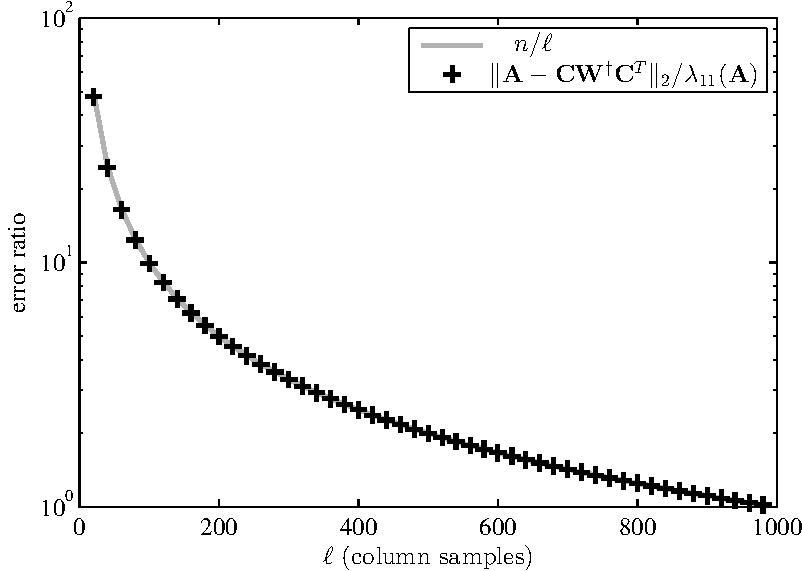
\includegraphics[width=6in,keepaspectratio=true]{%
figures/ch4/optimalityverification.pdf}
 \caption[Empirical demonstration of the optimality of Theorem~\ref{ch4:thm:uniformnystromerror}.]{
 {\sc Empirical demonstration of the optimality of Theorem~\ref{ch4:thm:uniformnystromerror}. } The empirical spectral-norm error of Nystr\"om extensions of
$\mat{A},$ the matrix defined in~\eqref{ch4:eqn:worsecaseA}, relative to the
spectral-norm error of the optimal rank-10 approximation of $\matA$. Each
point is the worst relative error observed in 60 trials. The ratio $n/\ell$ is
plotted; this is the dependence on $n$ and $\ell$ of the bound given in
Theorem~\ref{ch4:thm:uniformnystromerror}.}
 \label{ch4:fig:optimality}
\end{figure}


\subsection{Dependence on coherence}
In the following experiments, we use $500 \times 500$ matrices $\mat{A}$ with
eigendecompositions of the form
\begin{equation}
\mat{A} = [\begin{matrix} \mat{U}_1 & \mat{U}_2 \end{matrix}] 
 \left[ \begin{matrix} \mat{\Sigma}_1 & \\ & \mat{\Sigma}_2 \end{matrix} \right]
 \left[ \begin{matrix} \mat{U}_1\transp \\ \mat{U}_2\transp \end{matrix} \right]
 \label{ch4:eqn:coherenceA}
\end{equation}
where $\mat{U}_1$ is a $500 \times 10$ matrix with orthonormal columns and
specified coherence and the matrix $\mat{U}_2$ is chosen so that
$[\begin{matrix} \mat{U}_1 & \mat{U}_2 \end{matrix}]$ is an orthogonal matrix.
The 20 largest eigenvalues of $\mat{A}$ range logarithmically from $10$ to
$10^{-3},$ and the remaining eigenvalues are identically $10^{-15}.$ Routines
from the \textit{kappaSQ} Matlab package introduced in~\cite{IW12} are used to
generate $\mat{U}_1$ with specified coherences. For each value of coherence, we
consider two types of matrices $\mat{U}_1$ achieving this coherence: dense $\mat{U}_1$,
in which many rows of $\mat{U}_1$ are nonzero, and sparse $\mat{U}_1$, in which
many rows of $\mat{U}_1$ are zero. Dense $\mat{U}_1$ are generated using the
\texttt{mtxGenMethod1} routine, and sparse $\mat{U}_1$ are generated using the
\texttt{mtxGenMethod3} routine.

We compare the accuracies of regularized Nystr\"om extensions constructed using
Algorithm~\ref{ch4:alg:simple-stable-nystrom},
 to those of regularized Nystr\"om extensions constructed using
Algorithm~\ref{ch4:alg:CD11}. In Figure~\ref{ch4:fig:vary-coherence} we plot the ratio
of the approximation errors of the two regularized Nystr\"om extensions to the approximation
error of the optimal rank-10 approximant, as the coherence and sparsity of
$\mat{U}_1$ vary.
The regularization parameter $\rho$ is assigned the value
$\lambda_{11}(\mat{A}).$

\begin{figure}[htb!]
\centering
 \subfigure[Relative spectral-norm errors of
Algorithm~\ref{ch4:alg:simple-stable-nystrom}]{%
 
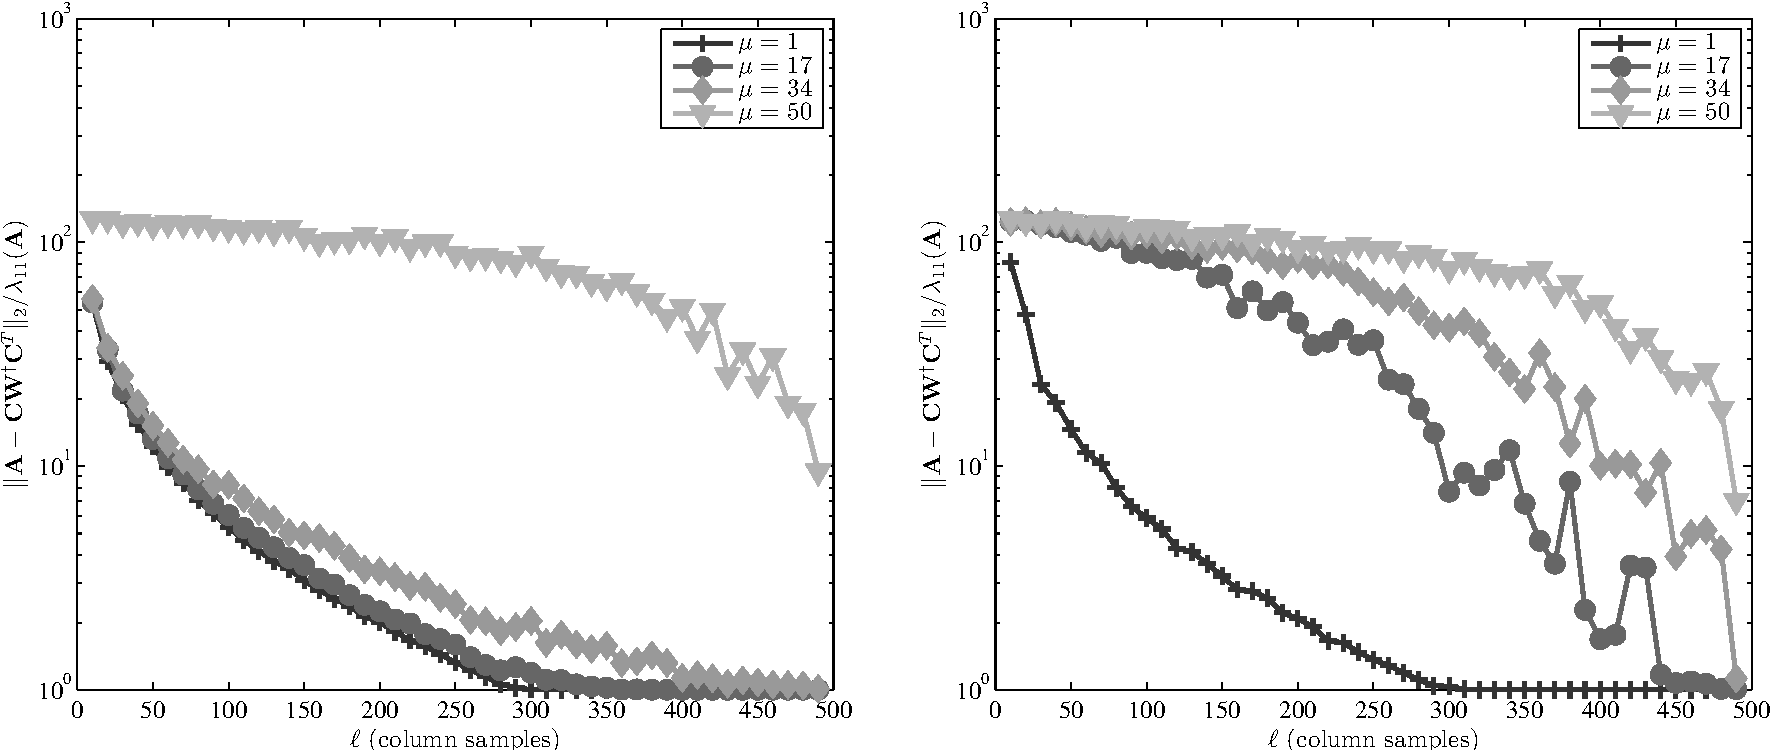
\includegraphics[height=2.3in,keepaspectratio=true]{%
figures/ch4/RegularizedADenseVsSparse.pdf}
}


\subfigure[Relative spectral-norm errors of Algorithm~\ref{ch4:alg:CD11}]{%
 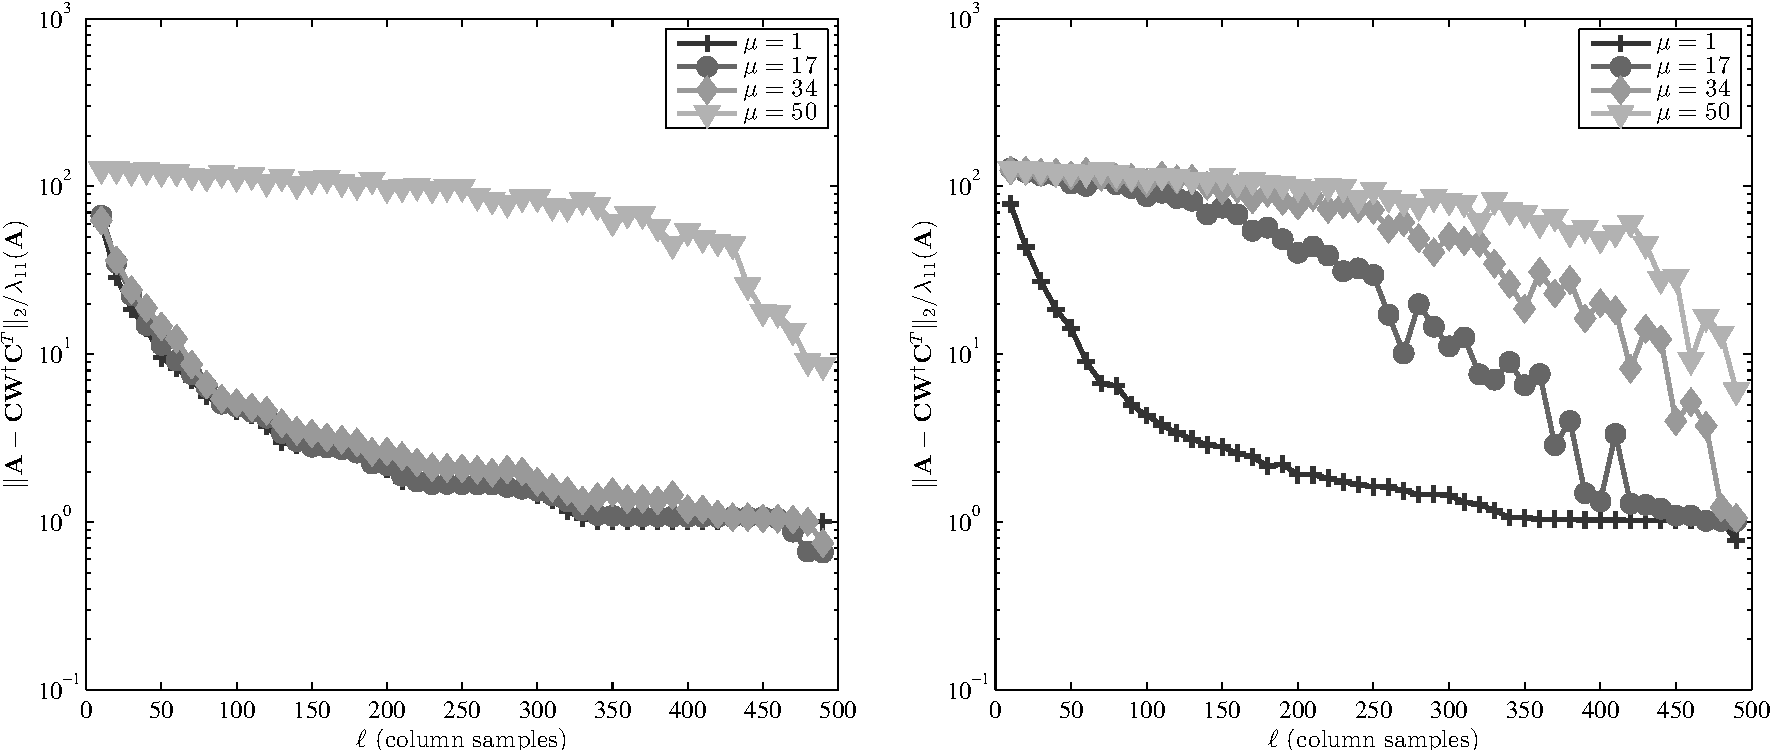
\includegraphics[height=2.3in,keepaspectratio=true]{%
figures/ch4/TruncatedWDenseVsSparse.pdf}
}

\caption[Spectral-norm errors of regularized Nystr\"om extensions as coherence varies]{%
{\sc Spectral-norm errors of regularized Nystr\"om extensions as coherence varies.} 
The relative spectral-norm errors of Nystr\"om extensions of $\mat{A},$
the matrix defined in~\eqref{ch4:eqn:coherenceA}, generated using
Algorithms~\ref{ch4:alg:simple-stable-nystrom} and~\ref{ch4:alg:CD11},
as a function of the coherence of the dominant
10-dimensional eigenspace. The errors are measured relative to the error of the
optimal rank-10 approximation, and averaged over 60 runs for each value of
$\ell.$ The eigenvectors spanning the dominant eigenspace of the matrices used
in the experiments on the left-hand side are dense, and the corresponding
eigenvectors of the matrices used in the experiments on the right-hand side are
sparse. The coherences range from the minimum possible, 1, to the maximum of
50.}
\label{ch4:fig:vary-coherence}
\end{figure}

Both algorithms perform as suggested by Theorem~\ref{ch4:thm:uniformnystromerror}: as the coherence of the top
$k$-dimensional eigenspace increases, the number of samples needed to obtain a small relative
error increases. Additionally, Figure~\ref{ch4:fig:vary-coherence} shows that the
structure of the eigenvectors is as important as the coherence of the
eigenspace: when the eigenvectors are dense, the number of samples needed to
obtain a small relative error is much less sensitive to the coherence than when
the eigenvectors are sparse. That is, for a fixed coherence and number of column
samples, the Nystr\"om extensions give lower errors when the eigenvectors are
dense than they do when the eigenvectors are sparse. 

\subsection*{Dependence on the regularization parameter}
Both algorithms require the choice of a regularization parameter
$\rho.$ In Figure~\ref{ch4:fig:regularization}, we observe the effect of the
regularization parameter $\rho$ on the errors of the Nystr\"om extensions. Here
the matrix $\mat{A}$ is again a $500 \times 500$ matrix with eigendecomposition
\begin{equation}
\mat{A} = [\begin{matrix} \mat{U}_1 & \mat{U}_2 \end{matrix}] 
 \left[ \begin{matrix} \mat{\Sigma}_1 & \\ & \mat{\Sigma}_2 \end{matrix} \right]
 \left[ \begin{matrix} \mat{U}_1\transp \\ \mat{U}_2\transp \end{matrix}
\right],
 \label{ch4:eqn:rhodependencematrix}
\end{equation}
where $\mat{U}_1$ is a $500 \times 20$ matrix with orthonormal columns and
$\mat{U}_2$ is chosen so that $[\begin{matrix} \mat{U}_1 & \mat{U}_2
\end{matrix}]$ is an orthogonal matrix. The 40 dominant eigenvalues of $\mat{A}$
range logarithmically from $1$ to $10^{-10}$ and all remaining eigenvalues are
identically $10^{-10}.$ The \texttt{mtxGenMethod1} routine is used to construct
$\mat{U}_1$ with coherence 1. 

Figure~\ref{ch4:fig:regularization} shows the ratios of the spectral-norm 
errors of the Nystr\"om extension and the regularized extensions
computed by Algorithms~\ref{ch4:alg:simple-stable-nystrom} and~\ref{ch4:alg:CD11}
to the optimal rank-20 approximation error. The
number of columns used to form the extensions is fixed at $\ell = 200,$ 
and the regularization parameter is varied from the minimum possible value of 
1 to the maximum possible value of 50. We see
that both regularization algorithms exhibit the same behavior: for large
values of $\rho,$ they have higher error than the Nystr\"om extension; as
$\rho$ decreases, their errors become orders of magnitude smaller than that of
the Nystr\"om extension, and as $\rho$ continues to decrease, their
errors once again approach that of the Nystr\"om extension. This behavior
highlights the importance of choosing an appropriate regularization parameter:
if $\rho$ is too small then there is no benefit gained from the regularization,
and if it is too large then the 
regularization has a deliterious effect. We also observe that Algorithm~\ref{ch4:alg:CD11}
can be orders of magnitude more accurate than Algorithm~\ref{ch4:alg:simple-stable-nystrom}.

\begin{figure}[ht]
 \centering
 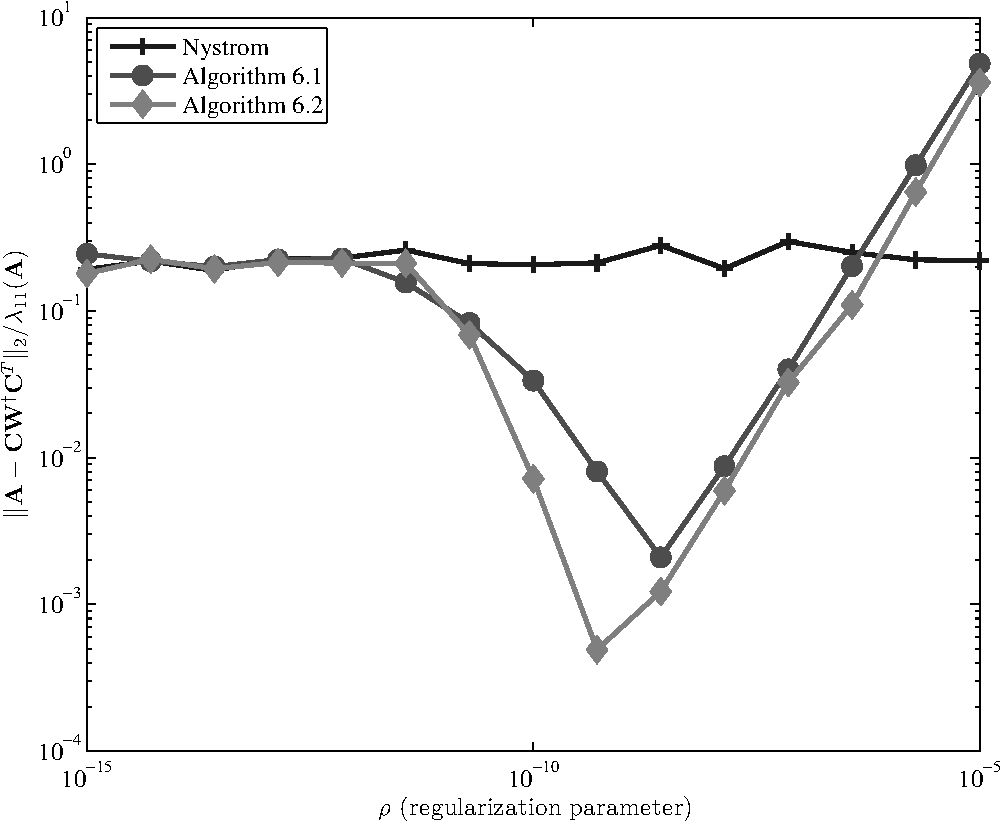
\includegraphics[width=6in,keepaspectratio=true]{%
figures/ch4/regularizationdependence.pdf}
 \caption[Spectral-norm error of regularized Nystr\"om extensions as regularization parameter varies]{%
{\sc Spectral-norm error of regularized Nystr\"om extensions as regularization parameter varies.} 
For the matrix $\mat{A}$ defined in~\eqref{ch4:eqn:rhodependencematrix},
the spectral-norm errors of the Nystr\"om extension and the extensions
generated using Algorithms~\ref{ch4:alg:simple-stable-nystrom}
and~\ref{ch4:alg:CD11}, as a function of
the regularization parameter $\rho.$ The errors are averaged over 60 runs for
each value of $\rho$ and plotted relative to the optimal spectral-norm rank-10 approximation error.}
 \label{ch4:fig:regularization}
\end{figure}


\section{Empirical aspects of SPSD low-rank approximation}
\label{ch4:sxn:emp}

In this section, we examine the empirical performance of the SPSD sketches
for which theoretical bounds were provided in Sections~\ref{ch4:sec:nystromextensions}
and~\ref{ch4:sec:mixturesketches}, on a diverse set of SPSD matrices.
% In addition to understanding the relative merits, in terms of both running 
% time and solution quality, of different sampling/projection schemes, we 
% would like to understand the effects of various data preprocessing decisions. 
% The bulk of our empirical evaluation considers two random projection
% procedures and two random sampling procedures for the sketching matrix 
% $\matS$:
% for random projections, we consider using SRFTs (Subsampled Randomized Fourier Transforms) as well as uniformly 
% sampling from Gaussian mixtures of the columns; and for random sampling, we 
% consider sampling columns uniformly at random as well as sampling 
% columns according to a nonuniform importance sampling distribution that 
% depends on the empirical statistical leverage scores.
% In the latter case of leverage score-based sampling, we also consider 
% the use of both the (na\"{i}ve and expensive) exact algorithm as well as 
% a (recently-developed fast) approximation algorithm.
%%
% Section~\ref{ch4:sxn:emp-datasets} starts with a brief description of 
% the data sets we consider; and then Section~\ref{ch4:sxn:emp-decisions} 
% briefly describes the effect of various data preprocessing decisions.
% Then, in Section~\ref{ch4:sxn:emp-reconstruction}, we present our main 
% results on reconstruction quality for the random sampling and random 
% projection methods; and, in Section~\ref{ch4:sxn:approx-levmethods}, we 
% discuss running time issues, and we present our main results for running time 
% and reconstruction quality for both exact and approximate versions of 
% leverage-based sampling.
% 
% We emphasize that we don't intend these results to be ``comprehensive'' but 
% instead to be ``illustrative'' case-studies---that are representative of a 
% much wider range of applications than have been considered previously.
% In particular, we would like to illustrate the tradeoffs between these 
% methods in different realistic applications in order, \emph{e.g.}, to provide 
% directions for future work.
% For instance, \emph{prima facie}, algorithms based on leverage-based column 
% sampling might be expected to be more expensive than those based on uniform 
% column sampling or random projections, but (based on previous work for general 
% matrices~\cite{DMM08CUR,DMMS11,MM11})
% they might also be expected to deliver lower approximation errors.
% Similarly, using approximate leverage scores to construct the importance 
% sampling distribution might be expected to perform worse than using exact 
% leverage scores, but this might be acceptable given its computational 
% advantages. 
% In addition to clarifying some of these issues, our empirical evaluation 
% also illustrates ways in which existing theory is insufficient to 
% explain the success of sampling and projection methods.
% This motivates our improvements to existing theory that we describe in 
% Section~\ref{sxn:theory}.

% With respect to our computation environment,
% all of our computations were conducted using 64-bit MATLAB R2012a under 
% Ubuntu on a 2.6--GHz quad-core Intel i7 machine with 6Gb of RAM. 
% To allow for accurate timing comparisons, all computations were carried out 
% in a single thread. 
% When applied to an $n \times n$ SPSD matrix $\mat{A}$, 
% our implementation of the SRFT requires $\mathrm{O}(n^2 \log n)$ operations, 
% as it applies MATLAB's \texttt{fft} to the entire matrix $\mat{A}$ and
% \emph{then} it samples $\ell$ columns from the resulting matrix. 
% We note that the SRFT computation can be made more competitive: a more rigorous 
% implementation of the SRFT algorithm could reduce this running time to 
% $\mathrm{O}(n^2 \log \ell)$; but due to the complexities involved in 
% optimizing pruned FFT codes, we did not pursue this~avenue. 


\subsection{Test matrices}
\label{ch4:sxn:emp-datasets}

Table~\ref{ch4:table:datasets} provides summary statistics for the test matrices used 
in our computational experiments. 
In order to illustrate the strengths and weaknesses of 
% the different sketches over a wide range of matrices, we consider four classes of matrices which are commonly 
encountered in machine learning and data analysis applications, we drawn our test
matrices from the following classes of matrices: 
\begin{itemize}
\item normalized Laplacians of very sparse graphs drawn from ``informatics graph'' 
applications;
\item dense matrices corresponding to linear kernels from machine learning 
applications;
\item dense matrices constructed from a Gaussian radial basis function kernel 
(RBFK); and
\item sparse RBFK matrices constructed using Gaussian radial basis functions, 
truncated to be nonzero only for nearest neighbors.
\end{itemize}
% Although not exhaustive, this collection of data sets represents a wide range of 
% data sets with very different (sparsity, spectral, leverage score, etc.) 
% properties that have been of interest recently not only in machine learning 
% but in data analysis more generally.

\begin{table}[t]
\centerline{%
\begin{tabular}{|l|c|l|l|l|}
\hline
Name & Description & n & d  & \%nnz \\
\hline
\hline
\multicolumn{4}{|c|}{Laplacian kernels} \\
\hline
HEP      & arXiv High Energy Physics collaboration graph & 9877  & NA  & 0.06 \\
GR       & arXiv General Relativity collaboration graph  & 5242  & NA  & 0.12 \\
Enron    & subgraph of the Enron email graph             & 10000 & NA  & 0.22 \\
Gnutella & Gnutella peer to peer network on Aug. 6, 2002 & 8717  & NA  & 0.09 \\
\hline
\hline
\multicolumn{3}{|c|}{Linear kernels} \\
\hline
Dexter  & bag of words                             & 2000 & 20000  & 83.8 \\
Protein & derived feature matrix for S. cerevisiae & 6621 & 357    & 99.7 \\
SNPs    & DNA microarray data from cancer patients & 5520 & 43     & 100 \\
Gisette & images of handwritten digits             & 6000 & 5000   & 100 \\
\hline
\hline
\multicolumn{3}{|c|}{Dense RBF kernels} \\
\hline
AbaloneD & physical measurements of abalones & 4177 & 8   & 100 \\
WineD    & chemical measurements of wine     & 4898 & 12  & 100 \\
%Kin8nm   & simulated dynamics of a robot arm & 8192 & 9   & 100 \\
%Spam     & word and character frequencies    & 4601 & 57  & 100 \\
\hline
\hline
\multicolumn{3}{|c|}{Sparse RBF kernels} \\
\hline
AbaloneS & physical measurements of abalones & 4177 & 8  & 82.9/48.1 \\
WineS    & chemical measurements of wine     & 4898 & 12 & 11.1/88.0 \\
\hline
\end{tabular}
}
\caption[Information on the SPSD matrices used in our empirical evaluations]{
{\sc Information on the SPSD matrices used in our empirical evaluations.} The matrices used in our empirical evaluation 
(\cite{LKF07}, \cite{KY04}, \cite{GGBD05}, \cite{GSPDK06}, 
\cite{Netal02}, \cite{Corke96}, \cite{UCIMachineLearningRepository}). 
Here, $n$ is the number of data points, and $d$ is the number of features in 
the input space before kernelization.
For Laplacian ``kernels,'' $n$ is the number of nodes in the graph (and thus 
there is no $d$ since the graph is ``given'' rather than ``constructed'').
The \%nnz for the Sparse RBF kernels depends on the $\sigma$ parameter; 
see Table~\ref{ch4:table:datasets_stats}.
}
\label{ch4:table:datasets}
\end{table}


We briefly review the construction of normalized graph Laplacians, 
linear kernel matrices, RBFK matrices, and sparse RBFK matrices.

Given a graph with weighted adjacency matrix $\mat{W}$, its normalized graph Laplacian is 
\[
  \mat{A} = \mat{I} - \mat{D}^{-1/2} \mat{W} \mat{D}^{-1/2},
\]
where $\mat{D}$ is the diagonal matrix of weighted degrees of the nodes of the
graph, i.e., $D_{ii} = \sum_{j \neq i} W_{ij}$.

The remaining classes of matrices are constructed using a set of 
data points $\vec{x}_1, \ldots, \vec{x}_n \in \R^d.$ The linear kernel 
matrix $\mat{A}$ corresponding to those points is given by
\[
 A_{ij} = \langle \vec{x}_i, \vec{x}_k \rangle.
\]
A Gaussian RBFK matrix $\mat{A}^\sigma$ corresponding to these same points
is given by
\[
 A_{ij}^\sigma = \exp\bigg(\frac{-\TNormS{\vec{x}_i -
\vec{x}_j}}{\sigma^2}\bigg),
\]
where $\sigma$, a nonnegative number, determines the scale of the kernel.
Informally, $\sigma$ defines the ``size scale'' over which pairs of 
points $\vec{x}_i$ and $\vec{x}_j$ ``see'' each other.
Typically $\sigma$ is determined by a global cross-validation criterion, as 
$\mat{A}^\sigma$ is generated for some specific machine learning task. Thus,
one may have no \emph{a priori} knowledge of the behavior of the 
spectrum or leverage scores of $\mat{A}^\sigma$ as $\sigma$ is varied. 
Accordingly, we consider Gaussian RBFK matrices with different values of $\sigma$. 
Finally, given the same data points, one
can construct sparse Gaussian RBFK matrices using the formula
\[
 A_{ij}^{(\sigma,\nu,C)} = \left[ \left( 1 - \frac{\TNorm{\vec{x}_i 
 - \vec{x}_j}}{C}\right)^\nu \right]^+ \cdot \exp\bigg(\frac{-\TNormS{\vec{x}_i -
\vec{x}_j}}{\sigma^2}\bigg),
\]
where $[x]^+ = \max\{0, x\}.$
When $\nu$ is larger than $(d+1)/2,$ this matrix is positive semidefinite; 
and as the cutoff point $C$ decreases this matrix becomes more 
sparse~\cite{Genton02}. 
For simplicity, in our experiments we fix 
$\nu = \lceil (d+1)/2 \rceil$ and $C = 3 \sigma$ and we vary $\sigma$.
As with the effect of varying $\sigma$, the effect of varying the 
sparsity parameter $C$ is not obvious \emph{a priori}. The parameter $C$ is typically chosen
according to a global criterion to ensure good performance at a specific machine learning 
task, without consideration for its effect on the spectrum or leverage 
scores of $A_{ij}^{(\sigma,\nu,C)}$.

\begin{table}[t]
\small
\centerline{%
\begin{tabular}{|l|l|l|l|l|l|l|}
\hline
Name & \%nnz 
     & $\Big\lceil\tfrac{\FNormS{\mat{A}}}{\TNormS{\mat{A}}} \Big\rceil$
     & $k$ 
     & $\tfrac{\lambda_{k+1}}{\lambda_k}$ 
     & $100 \tfrac{\FNorm{\mat{A} - \mat{A}_k}}{\FNorm{\mat{A}}}$  
     & \pbox{3cm}{$k$th-largest \\ leverage score} \\
\hline
\hline
% Laplacian data sets
HEP & 0.06 & 3078 & 20 & 0.998 & 7.8 & 0.261 \\ 
HEP & 0.06 & 3078 & 60 & 0.998 & 13.2 & 0.278 \\
GR & 0.12 & 1679 & 20 & 0.999 & 10.5 & 0.286 \\
GR & 0.12 & 1679 & 60 & 1 & 17.9  & 0.289 \\
Enron & 0.22 & 2588 & 20 & 0.997 & 7.77 & 0.492 \\
Enron & 0.22 & 2588 & 60 & 0.999 & 12.0 & 0.298 \\
Gnutella & 0.09 & 2757 & 20 & 1 & 8.1 & 0.381 \\
Gnutella & 0.09 & 2757 & 60 & 0.999 & 13.7 & 0.340 \\
\hline
\hline
% Linear data sets
Dexter  & 83.8 & 176 & 8  & 0.963 & 14.5 & 0.067 \\
Protein & 99.7 & 24  & 10 & 0.987 & 42.6 & 0.008 \\
SNPs    & 100  & 3   & 5  & 0.928 & 85.5 & 0.002 \\
Gisette & 100  & 4   & 12 & 0.90  & 90.1 & 0.005 \\
\hline
\hline
% Dense RBF data sets
AbaloneD (dense, $\sigma = .15$) & 100 & 41 & 20 & 0.992 & 42.1 & 0.087 \\
AbaloneD (dense, $\sigma = 1$)   & 100 & 4  & 20 & 0.935 & 97.8 & 0.012 \\
WineD (dense, $\sigma = 1$)      & 100 & 31 & 20 & 0.99  & 43.1 & 0.107 \\
WineD (dense, $\sigma = 2.1$)    & 100 & 3  & 20 & 0.936 & 94.8 & 0.009 \\
\hline
\hline
% Sparse RBF data sets
AbaloneS (sparse, $\sigma = .15$) & 82.9 & 400 & 20 & 0.989 & 15.4 & 0.232 \\
AbaloneS (sparse, $\sigma = 1$)   & 48.1 & 5   & 20 & 0.982 & 90.6 & 0.017 \\
WineS (sparse, $\sigma = 1$)      & 11.1 & 116 & 20 & 0.995 & 29.5 & 0.200 \\
WineS (sparse, $\sigma = 2.1$)    & 88.0   & 39  & 20 & 0.992 & 41.6 & 0.098 \\
\hline
\end{tabular}
}
\caption[Statistics of our test matrices]{{\sc Statistics of our test matrices.}
Summary statistics for the matrices from Table~\ref{ch4:table:datasets}
used in our computational experiments.}
\label{ch4:table:datasets_stats}
\end{table}

To illustrate the diverse range of properties exhibited by these four classes
of matrices, consider Table~\ref{ch4:table:datasets_stats}.
Several observations are particularly relevant to our
discussion below.
\begin{itemize}
\item
All of the Laplacian kernels drawn from informatics graph applications are 
extremely sparse in terms of number of nonzeros, and tend to have 
very slow spectral decay, as illustrated both by the quantity 
$\big\lceil\FNormS{\mat{A}}/\TNormS{\mat{A}}\big\rceil$ (this is the 
\emph{stable rank}, a numerically stable (under)estimate of the 
rank of $\mat{A}$ also utilized in Chaper~\ref{ch3}) as well as by the relatively small fraction of the 
Frobenius norm that is captured by the best rank-$k$ approximation to 
$\mat{A}$.
For the Laplacian kernels we considered two values of the rank parameter $k$ 
that were chosen (somewhat) arbitrarily; many of the results we report 
continue to hold qualitatively if $k$ is chosen to be (say) an order of 
magnitude larger. % but doing so tends to densify the low-rank approximation 
%to the Laplacian matrix.
\item
Both the linear kernels and the dense RBF kernels are much denser and are 
much more well-approximated by moderate to very low-rank matrices.
In addition, both the linear kernels and the dense RBF kernels have 
statistical leverage scores that are much more uniform---there are several 
ways to illustrate this, none of them perfect, and here, we illustrate this 
by considering the $k$th largest leverage score.
For the linear kernels and the dense RBF kernels, this quantity is one to
two orders of magnitude smaller than for the Laplacian kernels.
\item
For the dense RBF kernels, we consider two values of the $\sigma$ parameter, 
again chosen (somewhat) arbitrarily.
For both AbaloneD and WineD, we see that decreasing $\sigma$ from $1$ to 
$0.15$, i.e., letting data points ``see'' fewer nearby points, has two 
important effects:
first, it results in matrices that are much less well-approximated by 
low-rank matrices; and
second, it results in matrices that have much more heterogeneous leverage 
scores.
For example, for AbaloneD, the fraction of the Frobenius norm that is captured 
decreases from $97.8$ to $42.1$ and the $k$th largest leverage score 
increases from $0.012$ to~$0.087$.
\item
For the sparse RBF kernels, there are a range of sparsities, ranging from
above the sparsity of the sparsest linear kernel, but all are denser
than the Laplacian kernels.
Changing the $\sigma$ parameter has the same effect (although it is even 
more pronounced) for sparse RBF kernels as it has for dense RBF kernels.
In addition, ``sparsifying'' a dense RBF kernel also has the effect of 
making the matrix less well approximated by a low-rank matrix and of making
the leverage scores more nonuniform.
For example, for AbaloneD with $\sigma=1$ (respectively, $\sigma=0.15$), 
the fraction of the Frobenius norm that is captured decreases from $97.8$ 
(respectively, $42.1$) to $90.6$ (respectively, $15.4$), 
and the $k$th largest leverage score increases from $0.012$ 
(respectively, $0.087$) to $0.017$ (respectively,~$0.232$).
\end{itemize}
As we see below, when we consider the RBF kernels as the width parameter 
and sparsity are varied, we observe a range of intermediate cases between 
the extremes of linear kernels and Laplacian kernels.


\subsection{A comparison of empirical errors with the theoretical error bounds}

Table~\ref{ch4:table:theory-practice-gap} illustrates the gap between the theoretical results 
currently available in the literature, the bounds derived in this chapter, and what is observed in practice: it depicts the ratio
between the error bounds summarized in Table~\ref{ch4:table:bounds-comparison} and the average errors observed
over 10 trials of SPSD sketching. The error bound from~\cite{RT10} is not considered in the table,
as it does not apply at the number of samples $\ell$ used in the experiments. 

Several trends can be identified; among them, we
note that the bounds provided in this chapter for Gaussian-based sketches come quite close to capturing 
the errors seen in practice, and the Frobenius and trace-norm error guarantees of the 
leverage-based and Fourier-based sketches tend to more closely reflect the empirical behavior than
the error guarantees provided in prior work for Nystr\"om sketches. Overall, the trace-norm error
bounds are quite accurate. On the other hand, prior bounds are sometimes more informative in the case 
of the spectral norm (with the notable exception of the Gaussian sketches). Several important points
can be gleaned from these observations. 

First, the accuracy of the Gaussian error bounds suggests that the main theoretical
contribution of this work, the deterministic structural results given as 
Theorems~\ref{ch4:thm:colselection}, \ref{ch4:thm:frobenius-deterministic-error},
and~\ref{ch4:thm:trace-deterministic-error}, captures the underlying behavior of the SPSD sketching process. 
This supports our belief that our deterministic framework provides a foundation for truly 
informative error bounds. Second, it is clear that the 
analysis of the stochastic elements of the SPSD sketching process is 
much sharper in the Gaussian case than in the 
leverage-score, Fourier, and Nystr\"om cases. We expect that, at least in the 
case of leverage and Fourier-based sketches, the 
stochastic analysis can and will be sharpened to produce error guarantees 
almost as informative as the ones we have provided for
Gaussian-based sketches.

\begin{table}[!htb]
\centering
\begin{tabular}{|l|p{1in}|p{1in}|p{1in}|}
\hline
source, sketch
 & pred./obs. \linebreak spec. error
 & pred./obs. \linebreak Frob. error
 & pred./obs. \linebreak trace error \\
  \hline
  \multicolumn{4}{|c|}{Enron, $k = 60$ } \\
  \hline
% \cite{DM05}, Nystr\"om
%  & 3041
%  & 66.2
%  & -- \\
\cite{BW09}, Nystr\"om
 & --  
 & --  
 & 2.0\\
%\cite{TalRos10}, Nystr\"om
% & NA
% & NA
% & NA \\
\cite{KMT12}, Nystr\"om
 & 331.2
 & 77.7
 & -- \\
 Thm~\ref{ch4:thm:sample-lev},  leverage-based
 & 12888
 & 21
 & 1.2 \\
Thm~\ref{ch4:thm:proj-fourier}, Fourier-based
 & 201.0
 & 42.7
 & 1.6 \\
Thm~\ref{ch4:thm:proj-gaussian}, Gaussian-based
 & 10.1
 & 5.6
 & 1.2 \\
Thm~\ref{ch4:thm:uniformnystromerror}, Nystr\"om
 & 9.4
 & 385.2
 & 5.4 \\
 \hline
 \multicolumn{4}{|c|}{Protein, $k = 10$ }\\
 \hline
% \cite{DM05}, Nystr\"om
%  & 119.2 
%  & 18.6
%  & -- \\
\cite{BW09}, Nystr\"om
 & --  
 & --  
 & 3.6\\
%\cite{TalRos10}, Nystr\"om
% & NA
% & NA
% & NA \\
\cite{KMT12}, Nystr\"om
 & 33.4
 & 20.5
 & -- \\
Thm~\ref{ch4:thm:sample-lev},  leverage-based
 & 42.5
 & 6.9
 & 2.0 \\
Thm~\ref{ch4:thm:proj-fourier}, Fourier-based
 & 297.5
 & 21.7
 & 3.1\\
Thm~\ref{ch4:thm:proj-gaussian}, Gaussian-based
 & 3.8
 & 3.3
 & 1.8 \\
Thm~\ref{ch4:thm:uniformnystromerror}, Nystr\"om
 & 86.3
 & 91.3
 & 8 \\
 \hline
 \multicolumn{4}{|c|}{AbaloneD, $\sigma = .15, k = 20$ } \\
 \hline
% \cite{DM05}, Nystr\"om
%  & 349.9
%  & 42.5
%  & -- \\
\cite{BW09}, Nystr\"om
 & --  
 & --  
 & 2.0 \\
%\cite{TalRos10}, Nystr\"om
% & NA
% & NA
% & NA \\
\cite{KMT12}, Nystr\"om
 & 62.9
 & 46.7
 & -- \\
Thm~\ref{ch4:thm:sample-lev},  leverage-based
 & 235.3
 & 14.6
 & 1.3 \\
Thm~\ref{ch4:thm:proj-fourier}, Fourier-based
 & 139.4
 & 36.9
 & 1.7\\
Thm~\ref{ch4:thm:proj-gaussian}, Gaussian-based
 & 5.2
 & 4.7
 & 1.1\\
Thm~\ref{ch4:thm:uniformnystromerror}, Nystr\"om
 & 12.9
 & 228.3
 & 5.1\\
 \hline
 \multicolumn{4}{|c|}{WineS, $\sigma = 1, k = 20$ }\\
 \hline
%  \cite{DM05}, Nystr\"om
%  & 422.5
%  & 41.0
%  & -- \\
\cite{BW09}, Nystr\"om
 & --  
 & --  
 & 2.1\\
%\cite{TalRos10}, Nystr\"om
% & NA
% & NA
% & NA \\
\cite{KMT12}, Nystr\"om
 & 72.8
 & 44.2
 & -- \\
Thm~\ref{ch4:thm:sample-lev},  leverage-based
 & 244.9
 & 13.4
 & 1.2\\
Thm~\ref{ch4:thm:proj-fourier}, Fourier-based
 & 186.7
 & 36.8
 & 1.7\\
Thm~\ref{ch4:thm:proj-gaussian}, Gaussian-based
 & 6.6
 & 4.7
 & 1.2\\
Thm~\ref{ch4:thm:uniformnystromerror}, Nystr\"om
 & 13.7
 & 222.6
 & 5.1\\
 \hline
\end{tabular}
\caption[Comparison of empirical errors of SPSD sketches with predicted errors]{
{\sc Comparison of empirical errors of SPSD sketches with predicted errors.}
We compare the empirically observed approximation errors to the guarantees provided in this and other works, for several
matrices. Each approximation was formed using $\ell = 6 k\log k$ samples. To evaluate the error guarantees,
$\delta = 1/2$ was taken and all constants present in the statements of the bounds were replaced with ones. The observed errors were
taken to be the average errors over 10 runs of the approximation algorithms.
The matrices, described in Table~\ref{ch4:table:datasets}, are representative of several classes of matrices prevalent
in machine learning applications.}
\label{ch4:table:theory-practice-gap}
\end{table}


\subsection{Reconstruction accuracy of sampling and projection-based sketches}
\label{ch4:sxn:emp-reconstruction}

Here, we describe the performances of the various SPSD sketches in terms of 
reconstruction accuracy on the matrices described in 
Section~\ref{ch4:sxn:emp-datasets}. Recall that the sketches considered are
Nystr\"om extensions, leverage-based sketches, and sketches formed using 
Gaussian and SRFT mixtures of columns.

We describe general observations we have made about each class of 
matrices in turn, and then we summarize our observations.
We present results for both the rank-restricted and non-rank-restricted sketches.
That is, we plot the errors
\begin{equation}
\|\mat{A} - \mat{C} \mat{W}^\dagger \mat{C}\transp\|_\xi/\|\mat{A} - \mat{A}_k\|_\xi
\label{ch4:eqn:relerr1}
\end{equation}
for the non-rank-restricted sketches, and the errors 
\begin{equation}
\|\mat{A} - \mat{C} \mat{W}_k^\dagger \mat{C}\transp\|_\xi/\|\mat{A} - \mat{A}_k\|_\xi
\label{ch4:eqn:relerr2}
\end{equation}
for the rank-restricted sketches.

\subsubsection{Graph Laplacians}

\begin{figure}[htp]
 \centering
 \subfigure[GR, $k = 20$]{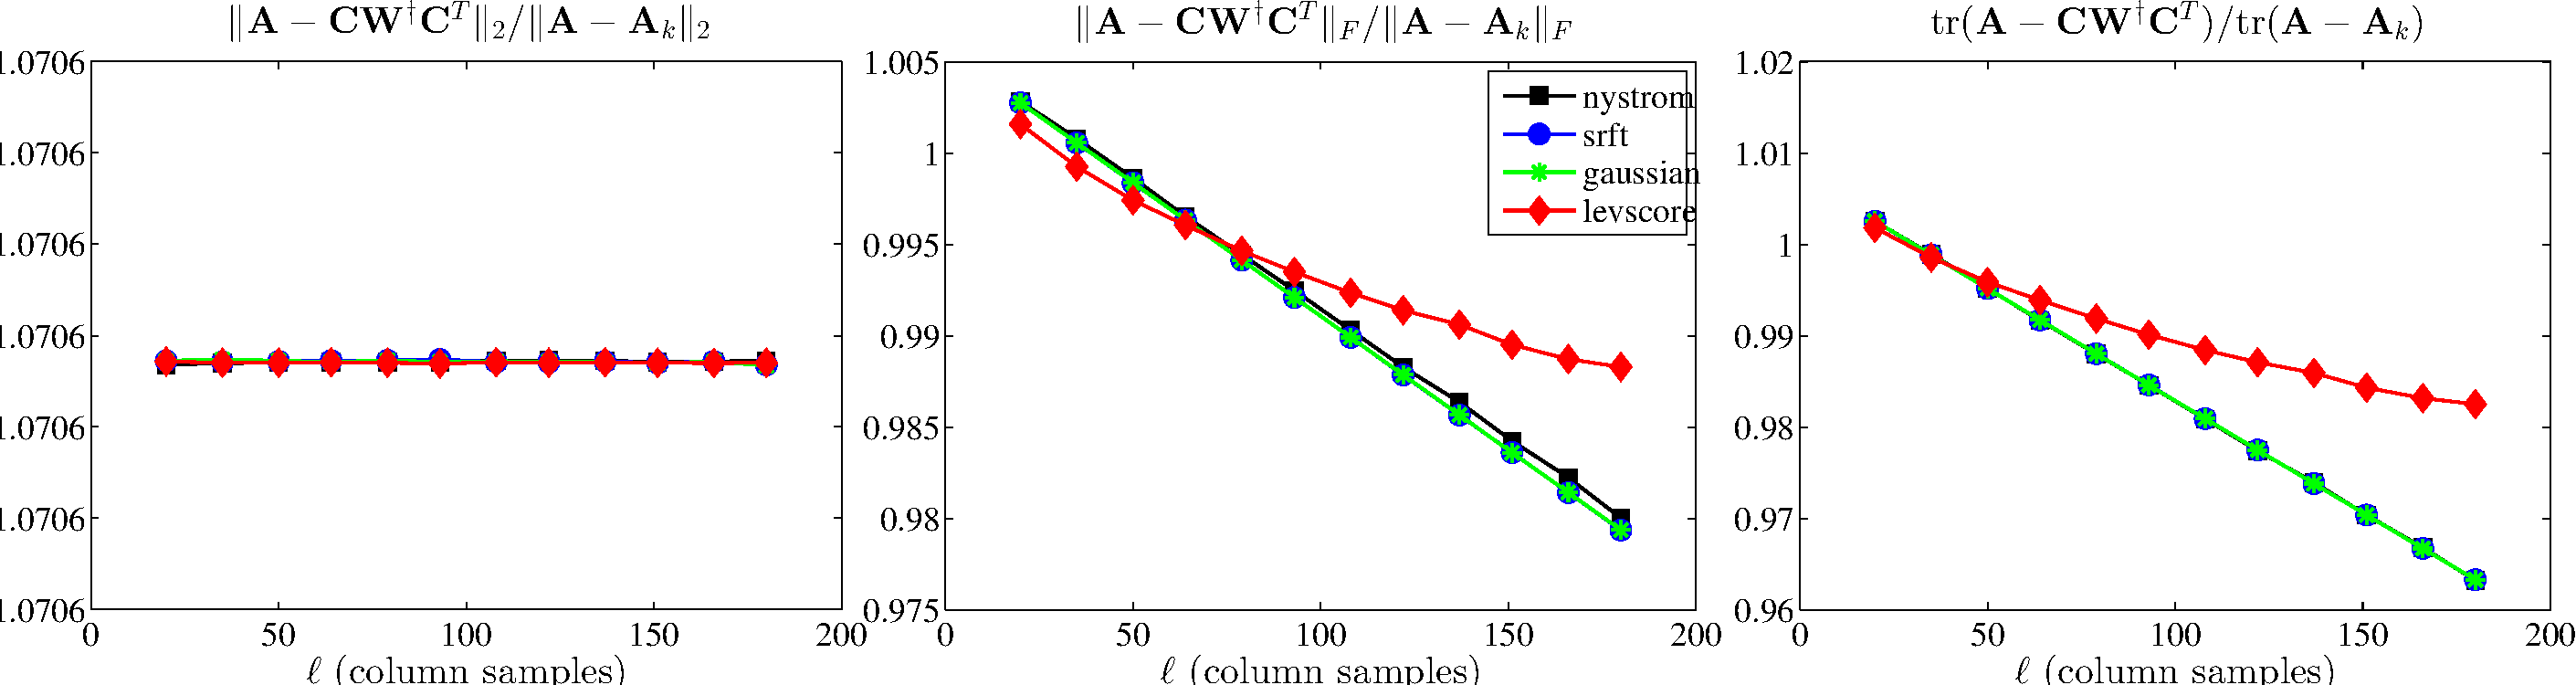
\includegraphics[width=6in, keepaspectratio=true]{figures/ch4/GRrank20exact-methods-nonfixed-rank-errors}}
 
 \subfigure[GR, $k = 60$]{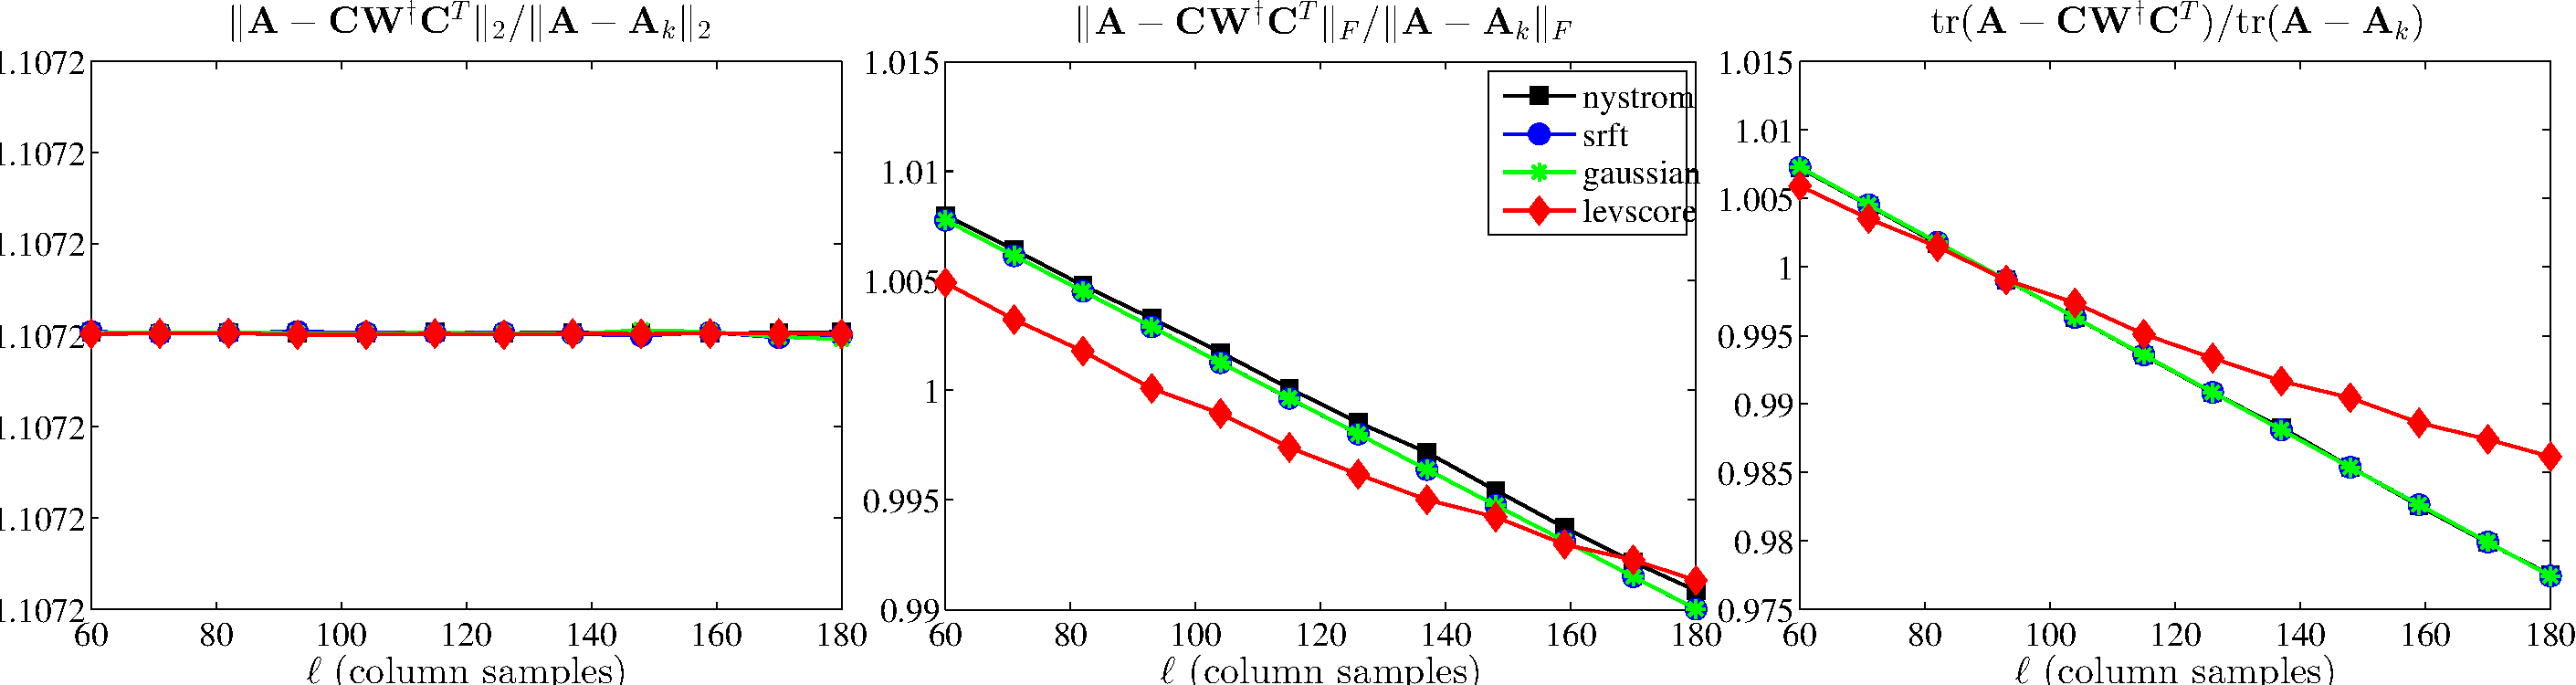
\includegraphics[width=6in, keepaspectratio=true]{figures/ch4/GRrank60exact-methods-nonfixed-rank-errors}}
 
 \subfigure[HEP, $k = 20$]{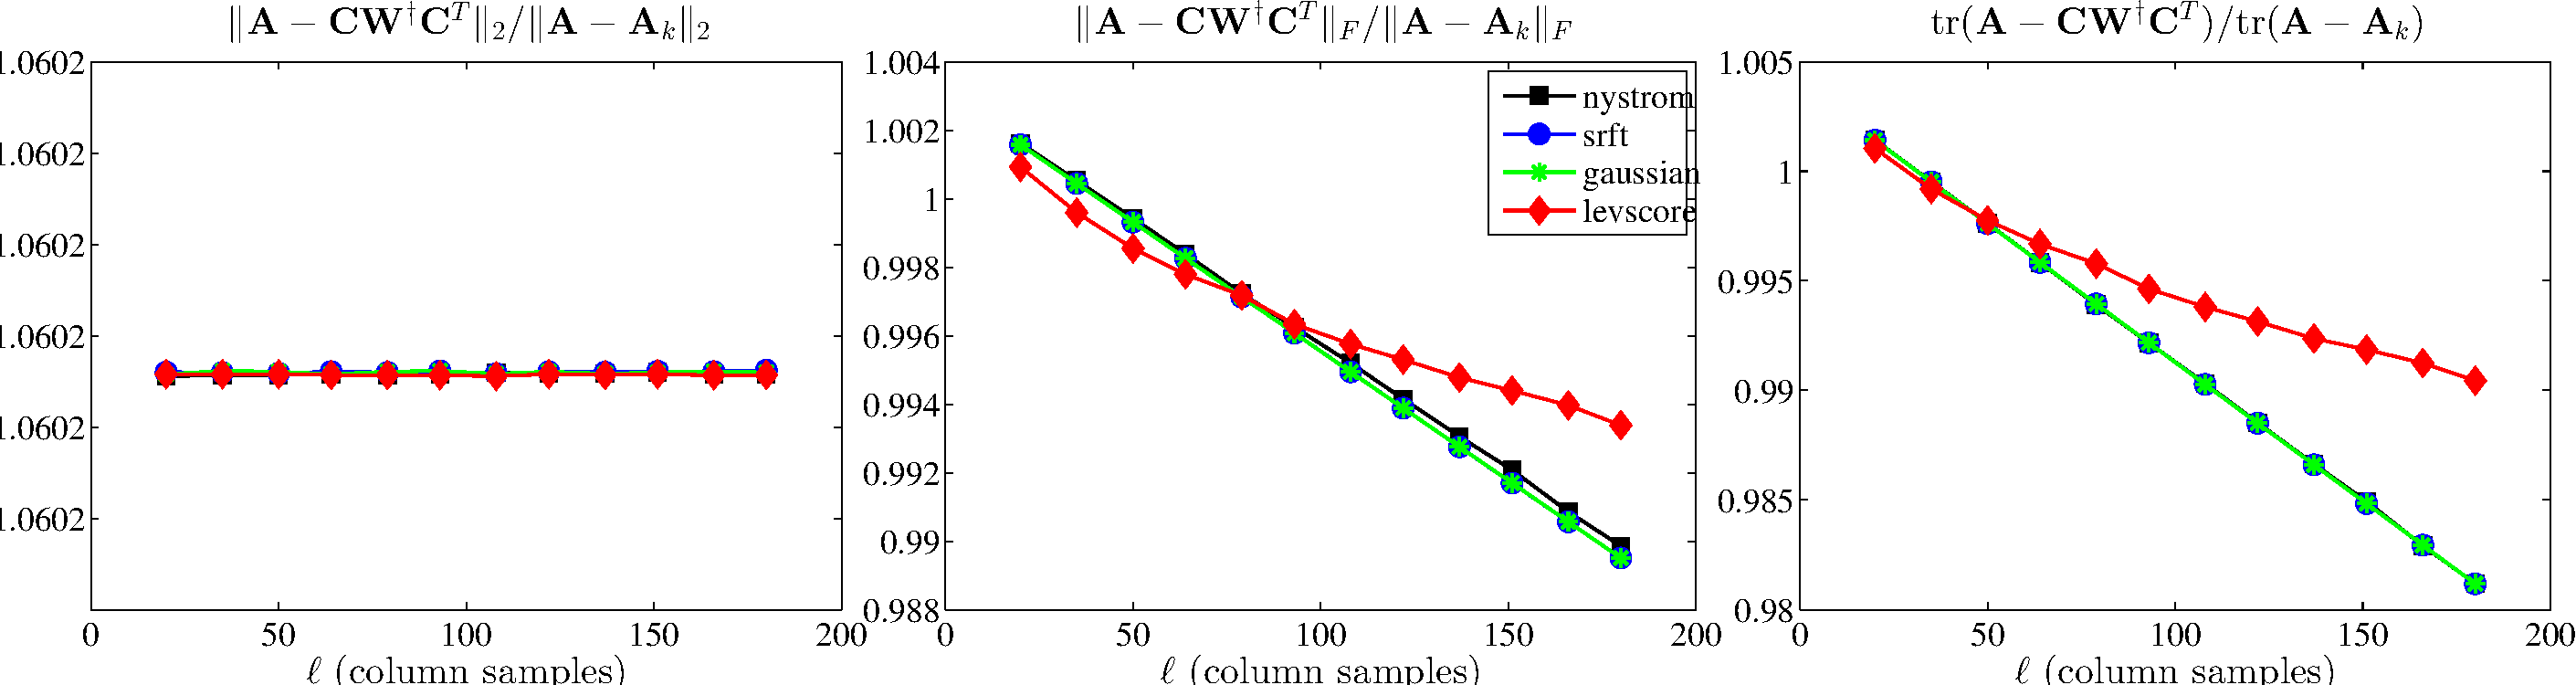
\includegraphics[width=6in, keepaspectratio=true]{figures/ch4/HEPrank20exact-methods-nonfixed-rank-errors}}
 
 \subfigure[HEP, $k = 60$]{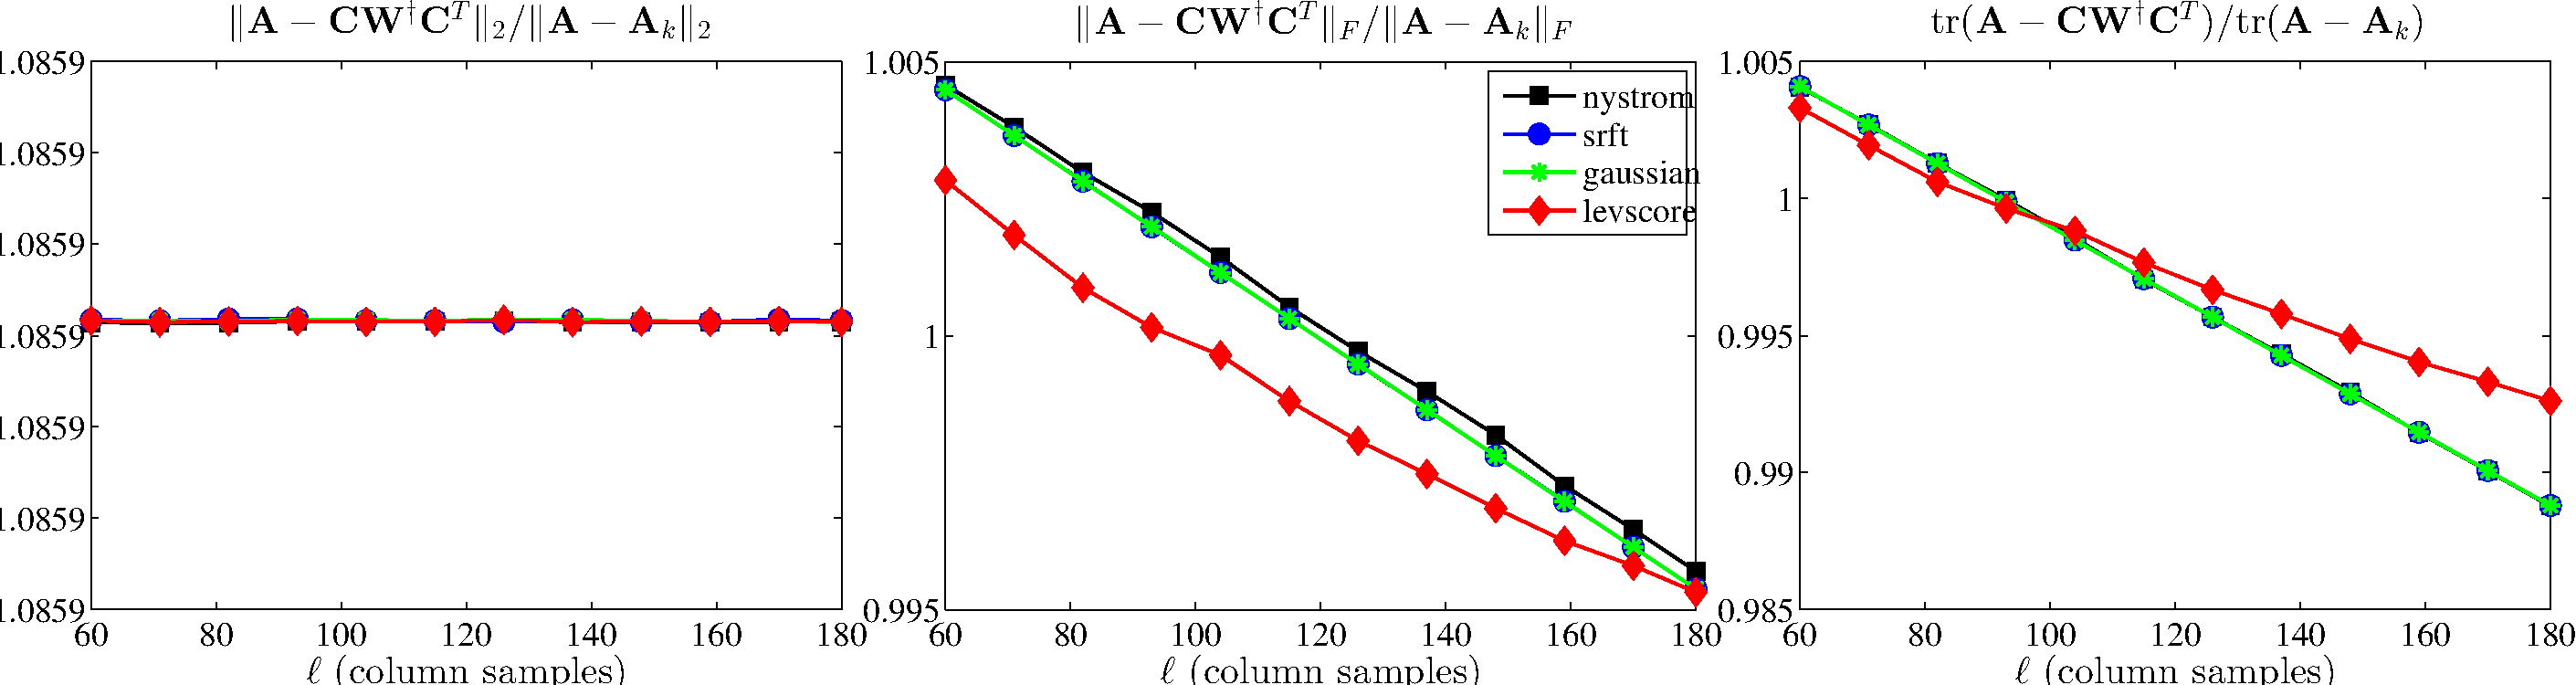
\includegraphics[width=6in, keepaspectratio=true]{figures/ch4/HEPrank60exact-methods-nonfixed-rank-errors}}%
  \caption[Relative errors of non-rank-restricted SPSD sketches of the GR and HEP Laplacian matrices]{%
 {\sc Relative errors of non-rank-restricted SPSD sketches of the GR and HEP Laplacian matrices.}
 The relative spectral, Frobenius, and trace-norm errors~\eqref{ch4:eqn:relerr1} of several non-rank-restricted
 SPSD sketches, as a function of the number of columns samples $\ell$, 
 for the GR and HEP Laplacian matrices, with two choices of the rank parameter $k$.}%
 \label{ch4:fig:laplacian-exact-errors-1a}
\end{figure}

\begin{figure}[htp]
 \centering
 \subfigure[Enron, $k = 20$]{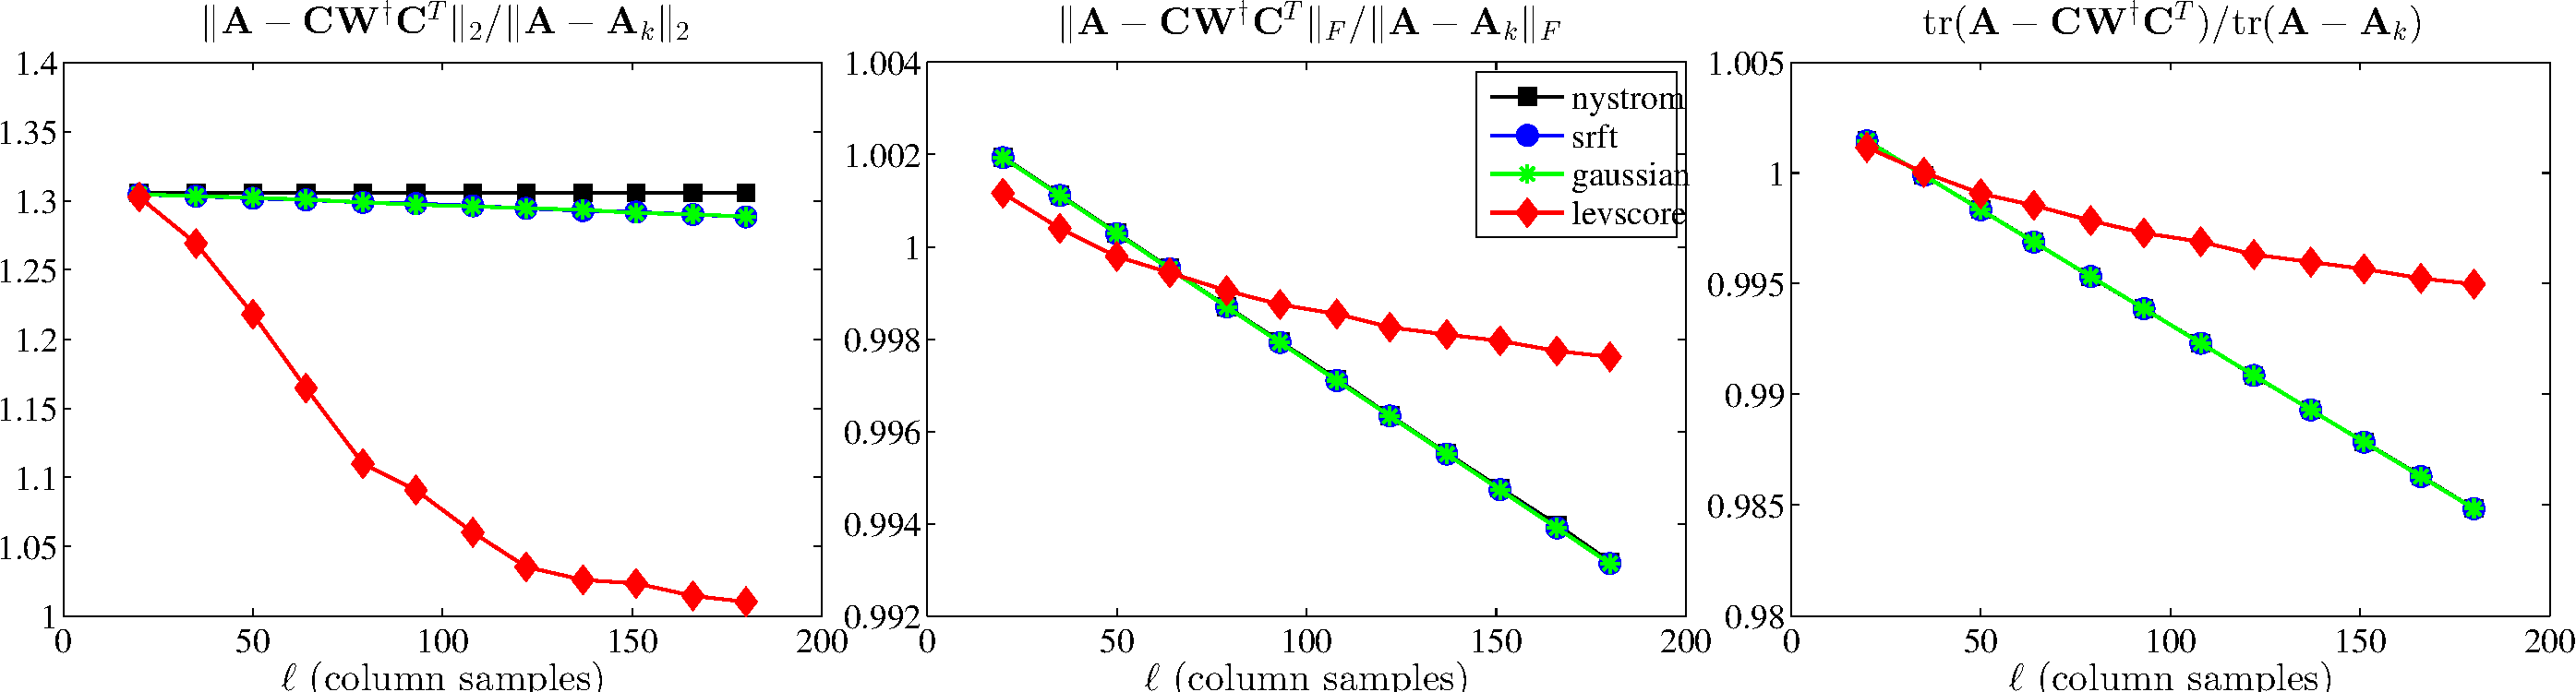
\includegraphics[width=6in, keepaspectratio=true]{figures/ch4/Enronrank20exact-methods-nonfixed-rank-errors}}
 
 \subfigure[Enron, $k = 60$]{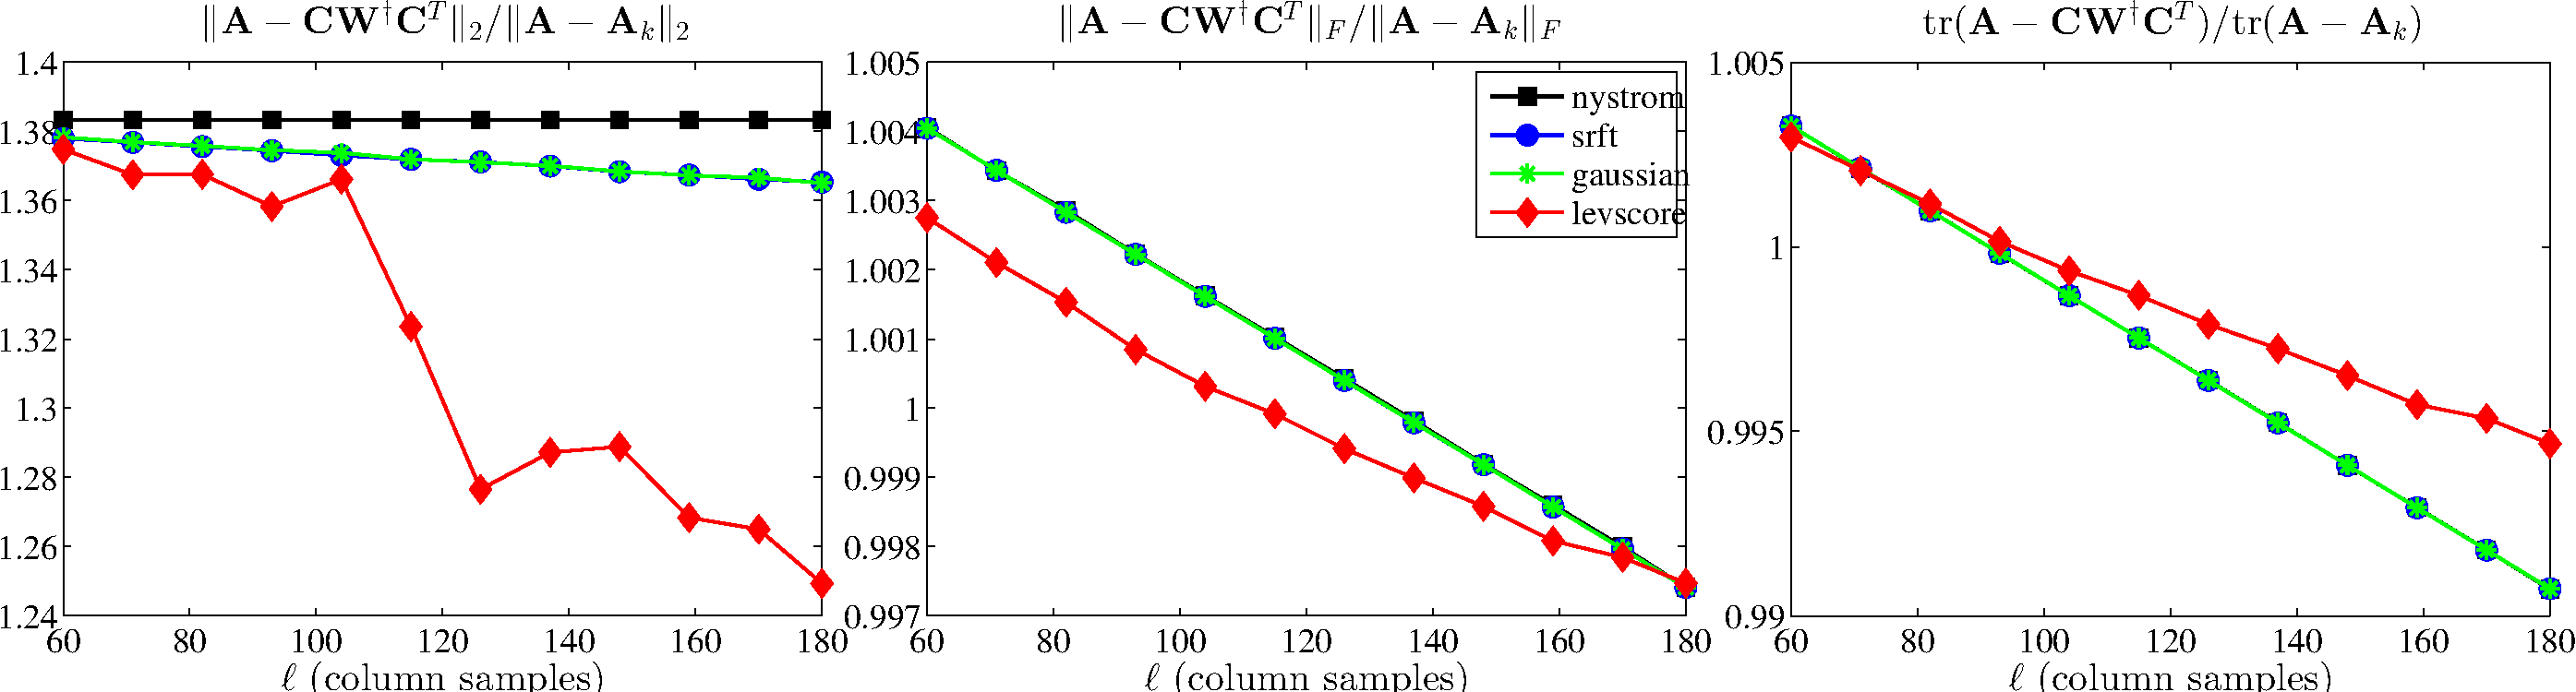
\includegraphics[width=6in, keepaspectratio=true]{figures/ch4/Enronrank60exact-methods-nonfixed-rank-errors}}
 
 \subfigure[Gnutella, $k = 20$]{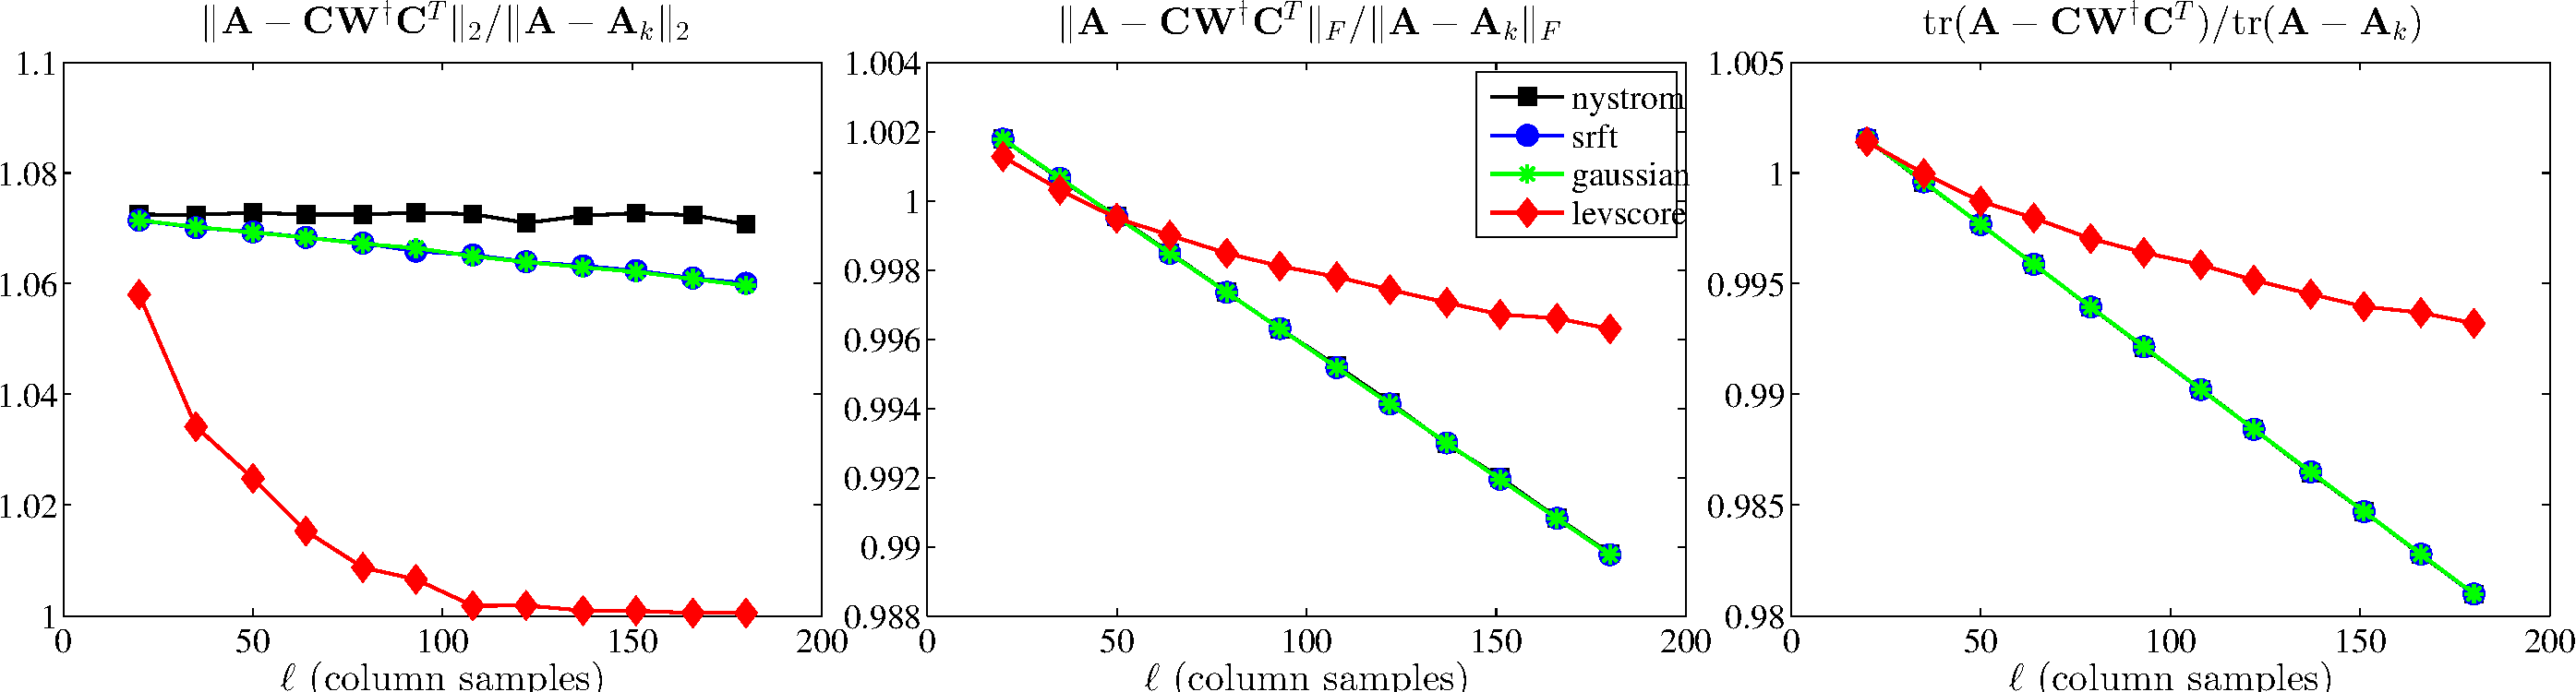
\includegraphics[width=6in, keepaspectratio=true]{figures/ch4/Gnutellarank20exact-methods-nonfixed-rank-errors}}
 
 \subfigure[Gnutella, $k = 60$]{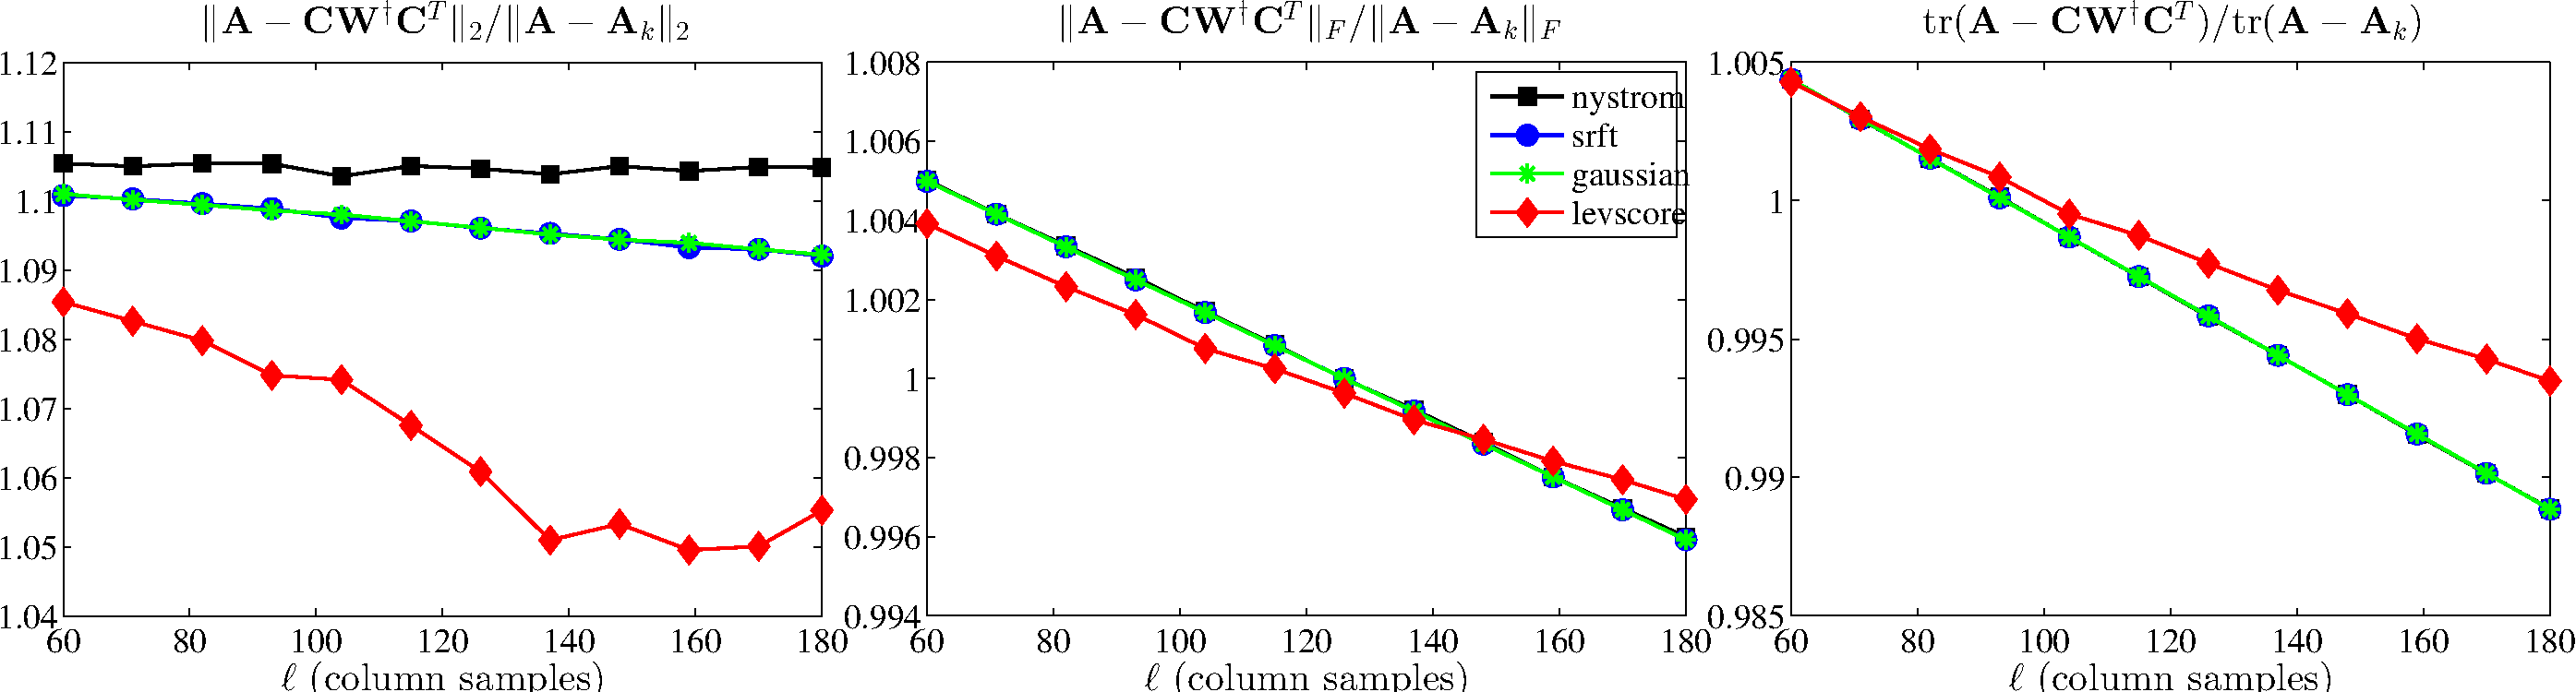
\includegraphics[width=6in, keepaspectratio=true]{figures/ch4/Gnutellarank60exact-methods-nonfixed-rank-errors}}
\caption[Relative errors of non-rank-restricted SPSD sketches of the Enron and Gnutella Laplacian matrices]{%
{\sc Relative errors of non-rank-restricted SPSD sketches of the Enron and Gnutella Laplacian matrices.}
 The relative spectral, Frobenius, and trace-norm errors~\eqref{ch4:eqn:relerr1} of several
 non-rank-restricted SPSD sketches, as a function of the number of columns samples $\ell$, 
 for the Enron and Gnutella Laplacian matrices, with two choices of the rank parameter $k$. }%
 \label{ch4:fig:laplacian-exact-errors-2a}
\end{figure}

\begin{figure}[htp]
 \centering
 \subfigure[GR, $k = 20$]{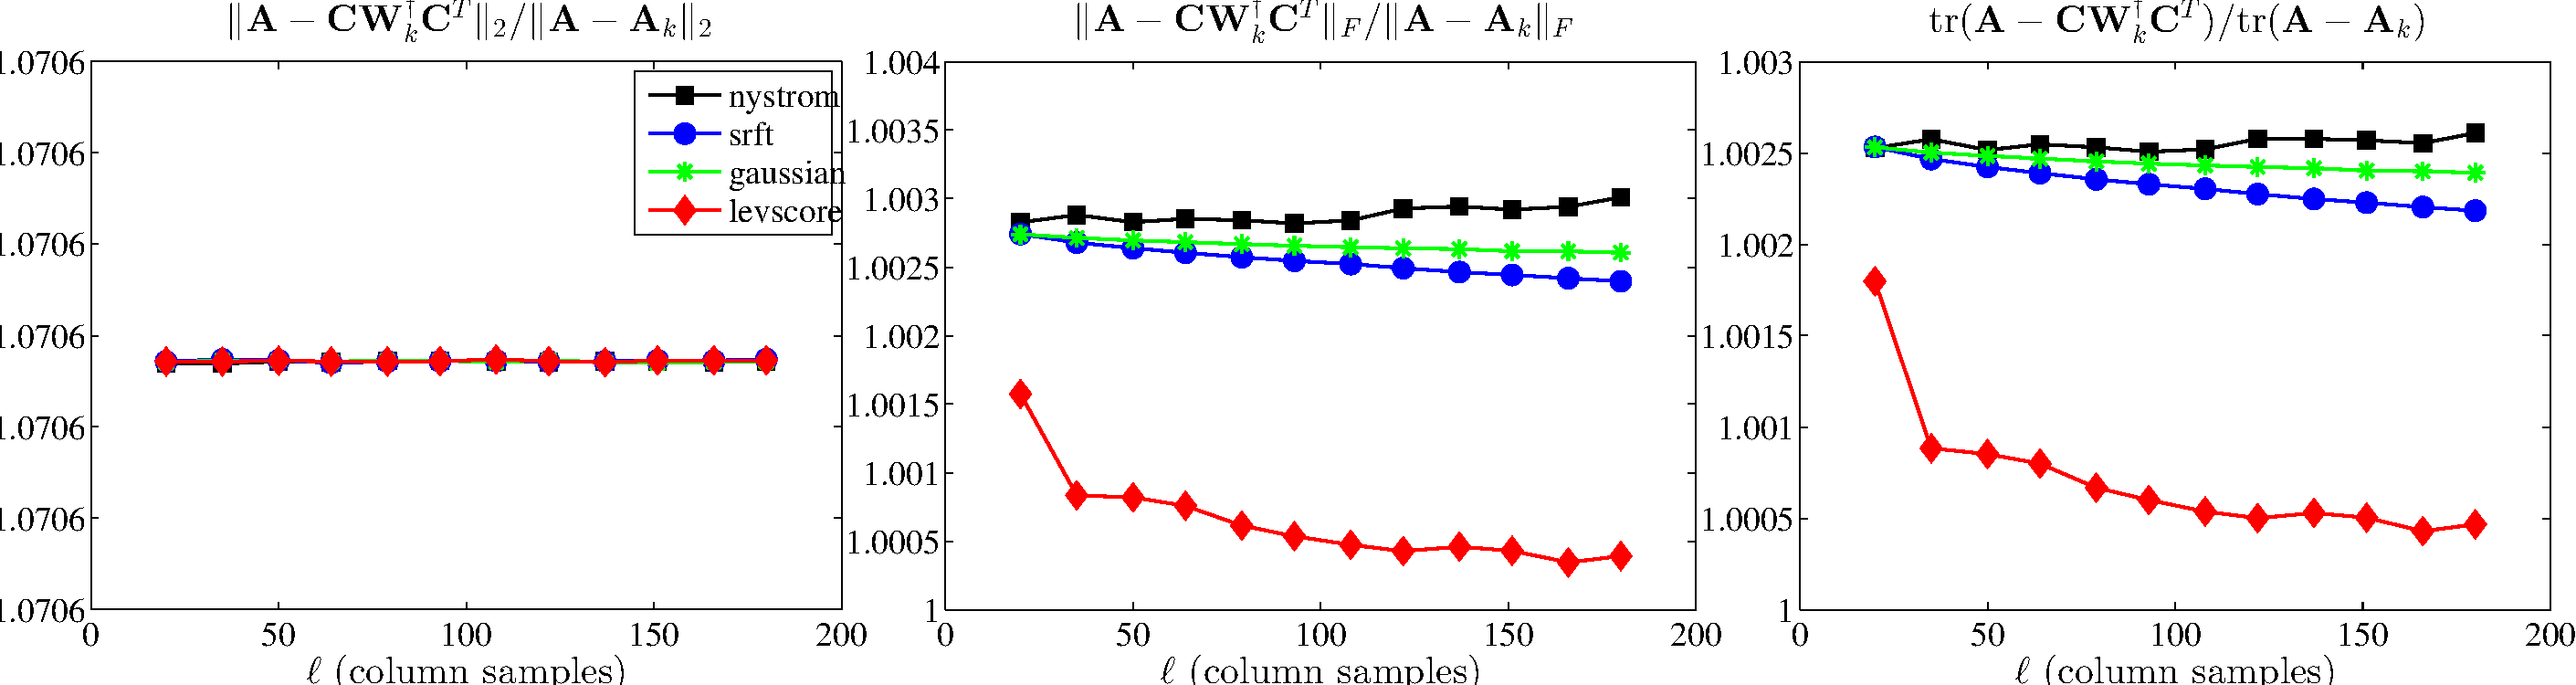
\includegraphics[width=6in, keepaspectratio=true]{figures/ch4/GRrank20exact-methods-fixed-rank-errors}}
 
 \subfigure[GR, $k = 60$]{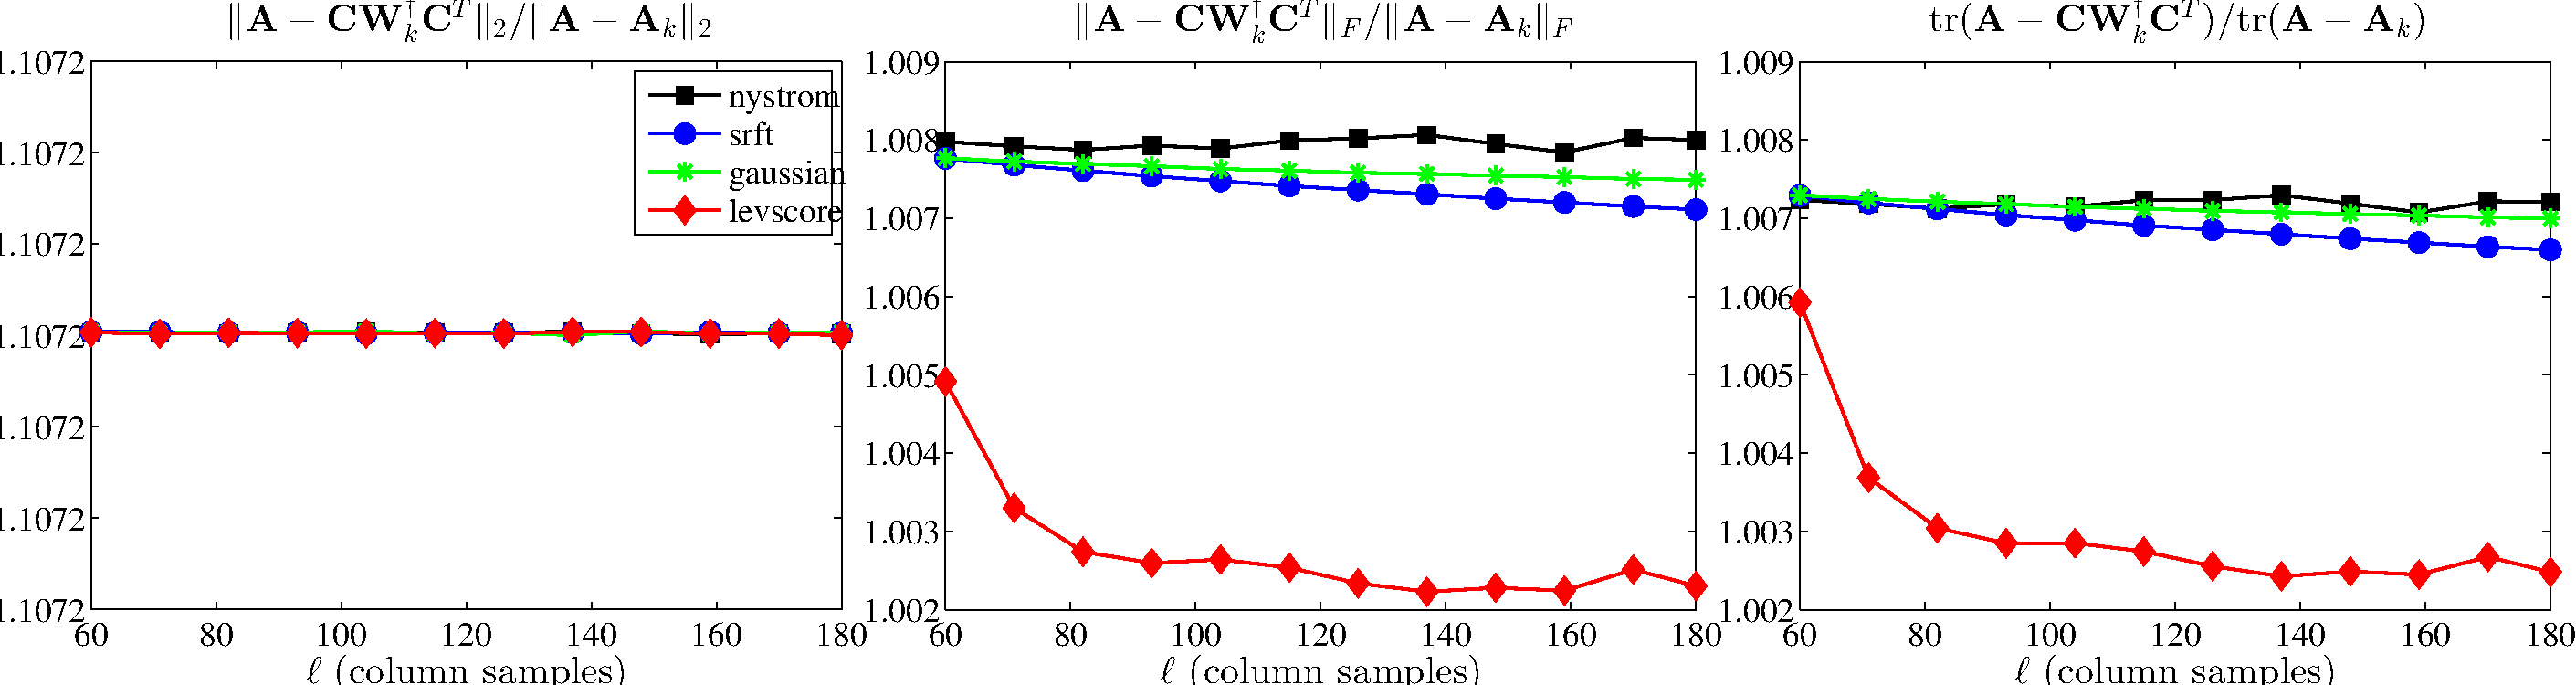
\includegraphics[width=6in, keepaspectratio=true]{figures/ch4/GRrank60exact-methods-fixed-rank-errors}}
 
 \subfigure[HEP, $k = 20$]{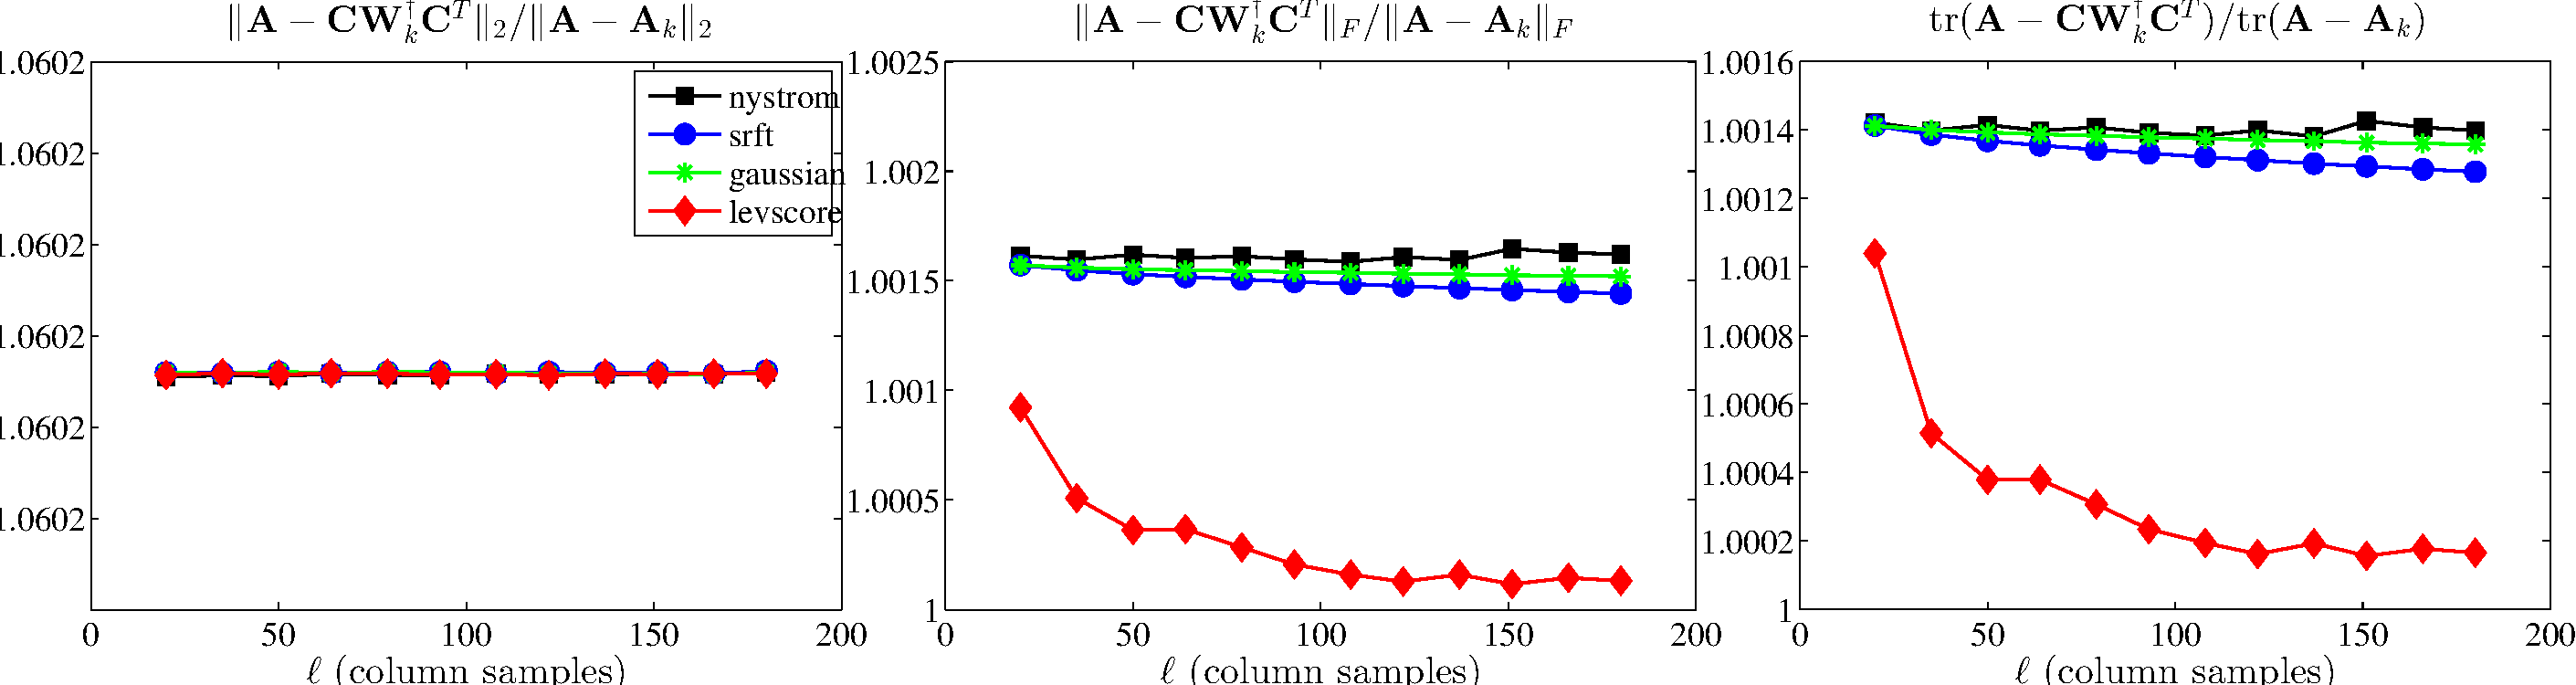
\includegraphics[width=6in, keepaspectratio=true]{figures/ch4/HEPrank20exact-methods-fixed-rank-errors}}
 
 \subfigure[HEP, $k = 60$]{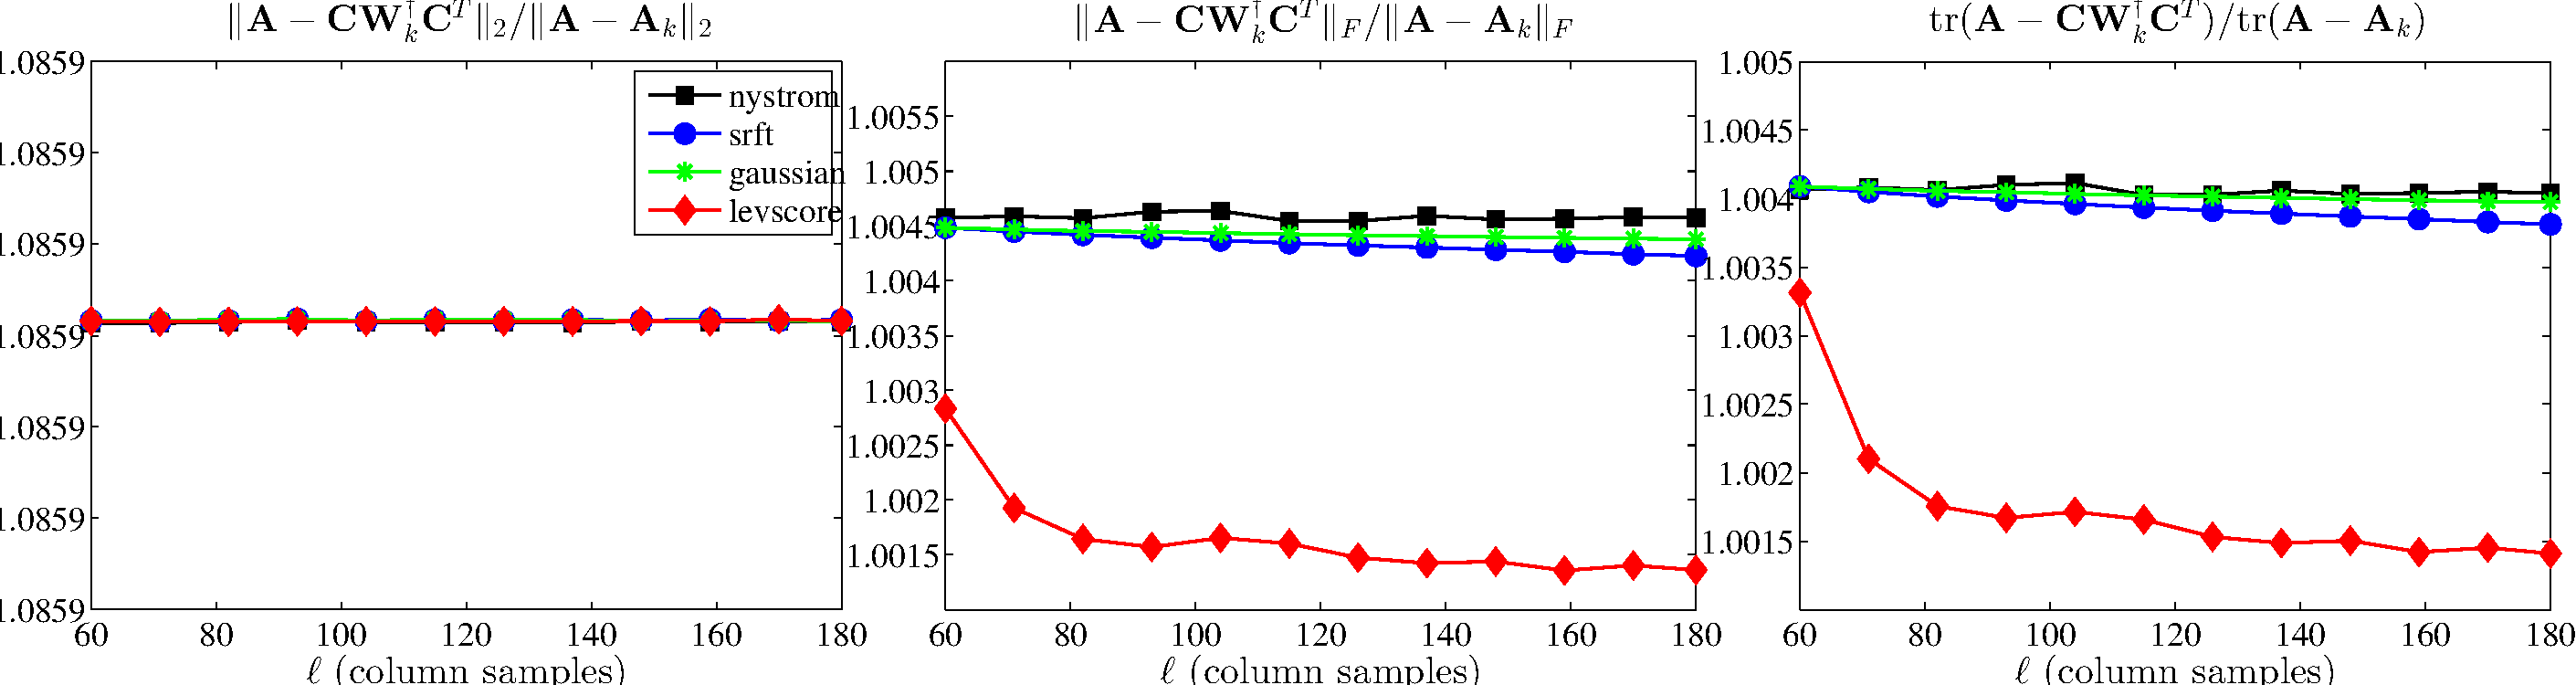
\includegraphics[width=6in, keepaspectratio=true]{figures/ch4/HEPrank60exact-methods-fixed-rank-errors}}
 \caption[Relative errors of rank-restricted SPSD sketches of the GR and HEP Laplacian matrices]{%
 {\sc Relative errors of rank-restricted SPSD sketches of the GR and HEP Laplacian matrices.}
 The relative spectral, Frobenius, and trace-norm errors~\eqref{ch4:eqn:relerr2} of several rank-restricted
 SPSD sketches, as a function of the number of columns samples $\ell$, 
 for the GR and HEP Laplacian matrices, with two choices of the rank parameter $k$.}%
 \label{ch4:fig:laplacian-exact-errors-1b}
\end{figure}

\begin{figure}[htp]
 \centering
 \subfigure[Enron, $k = 20$]{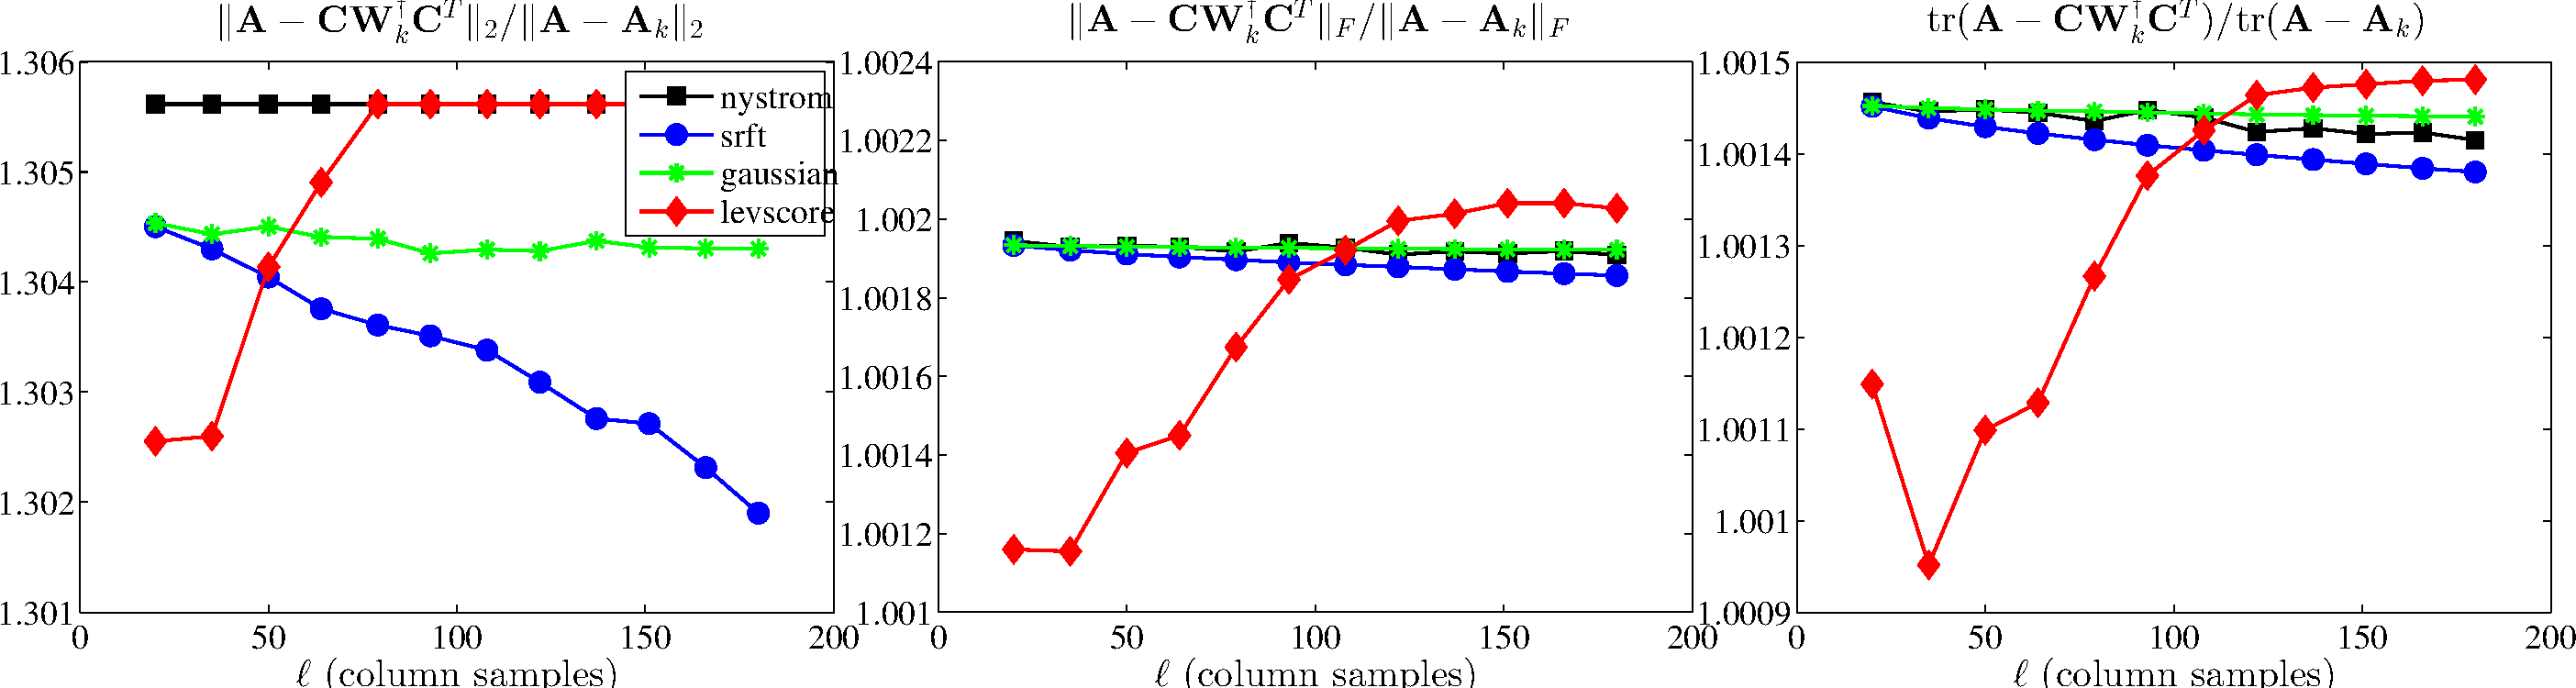
\includegraphics[width=6in, keepaspectratio=true]{figures/ch4/Enronrank20exact-methods-fixed-rank-errors}}
 
 \subfigure[Enron, $k = 60$]{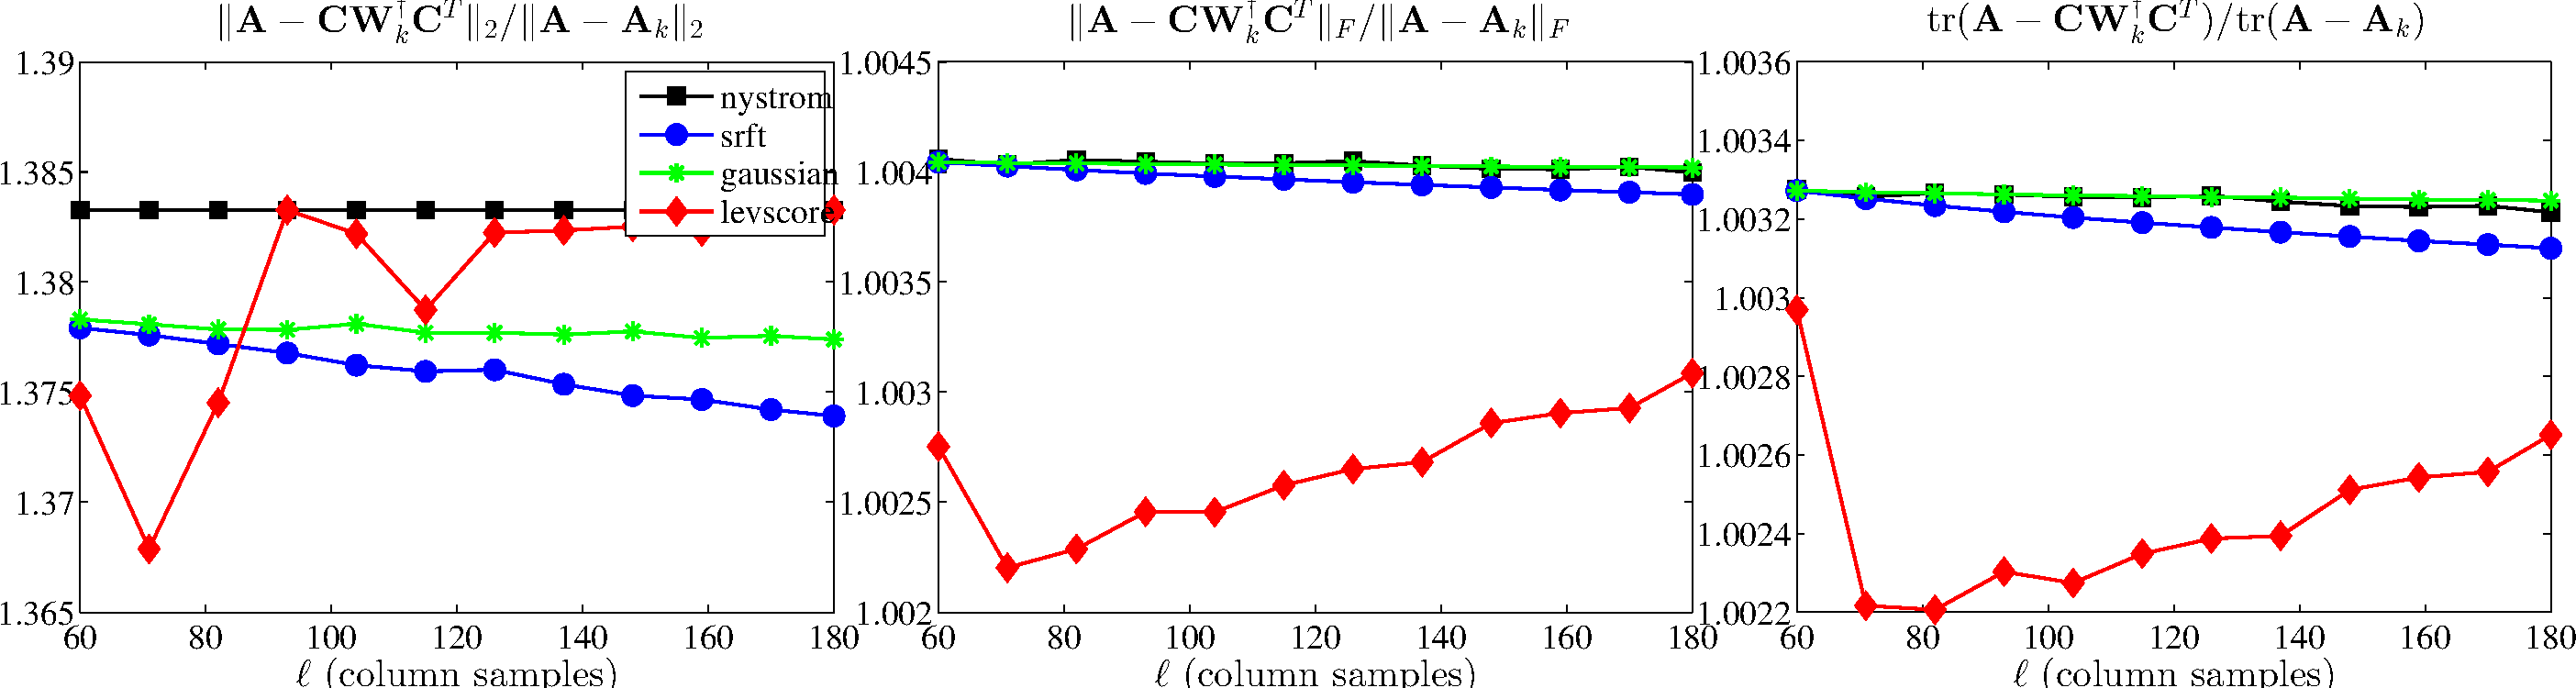
\includegraphics[width=6in, keepaspectratio=true]{figures/ch4/Enronrank60exact-methods-fixed-rank-errors}}
 
 \subfigure[Gnutella, $k = 20$]{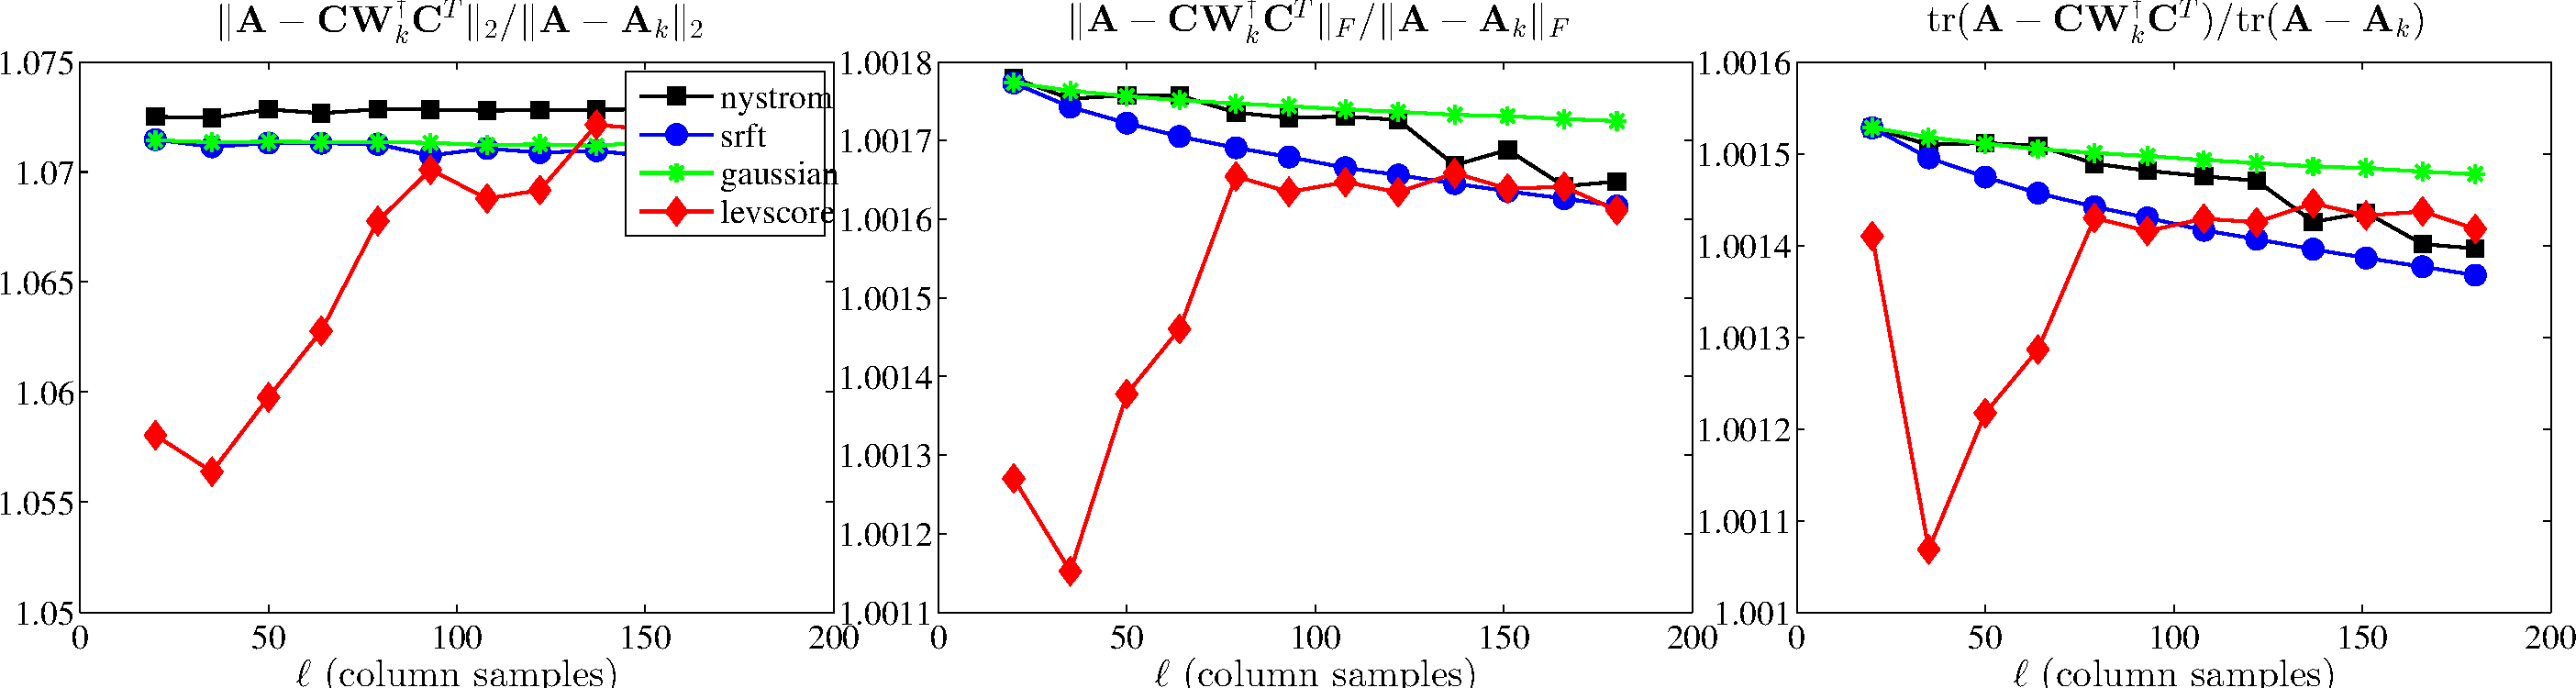
\includegraphics[width=6in, keepaspectratio=true]{figures/ch4/Gnutellarank20exact-methods-fixed-rank-errors}}
 
 \subfigure[Gnutella, $k = 60$]{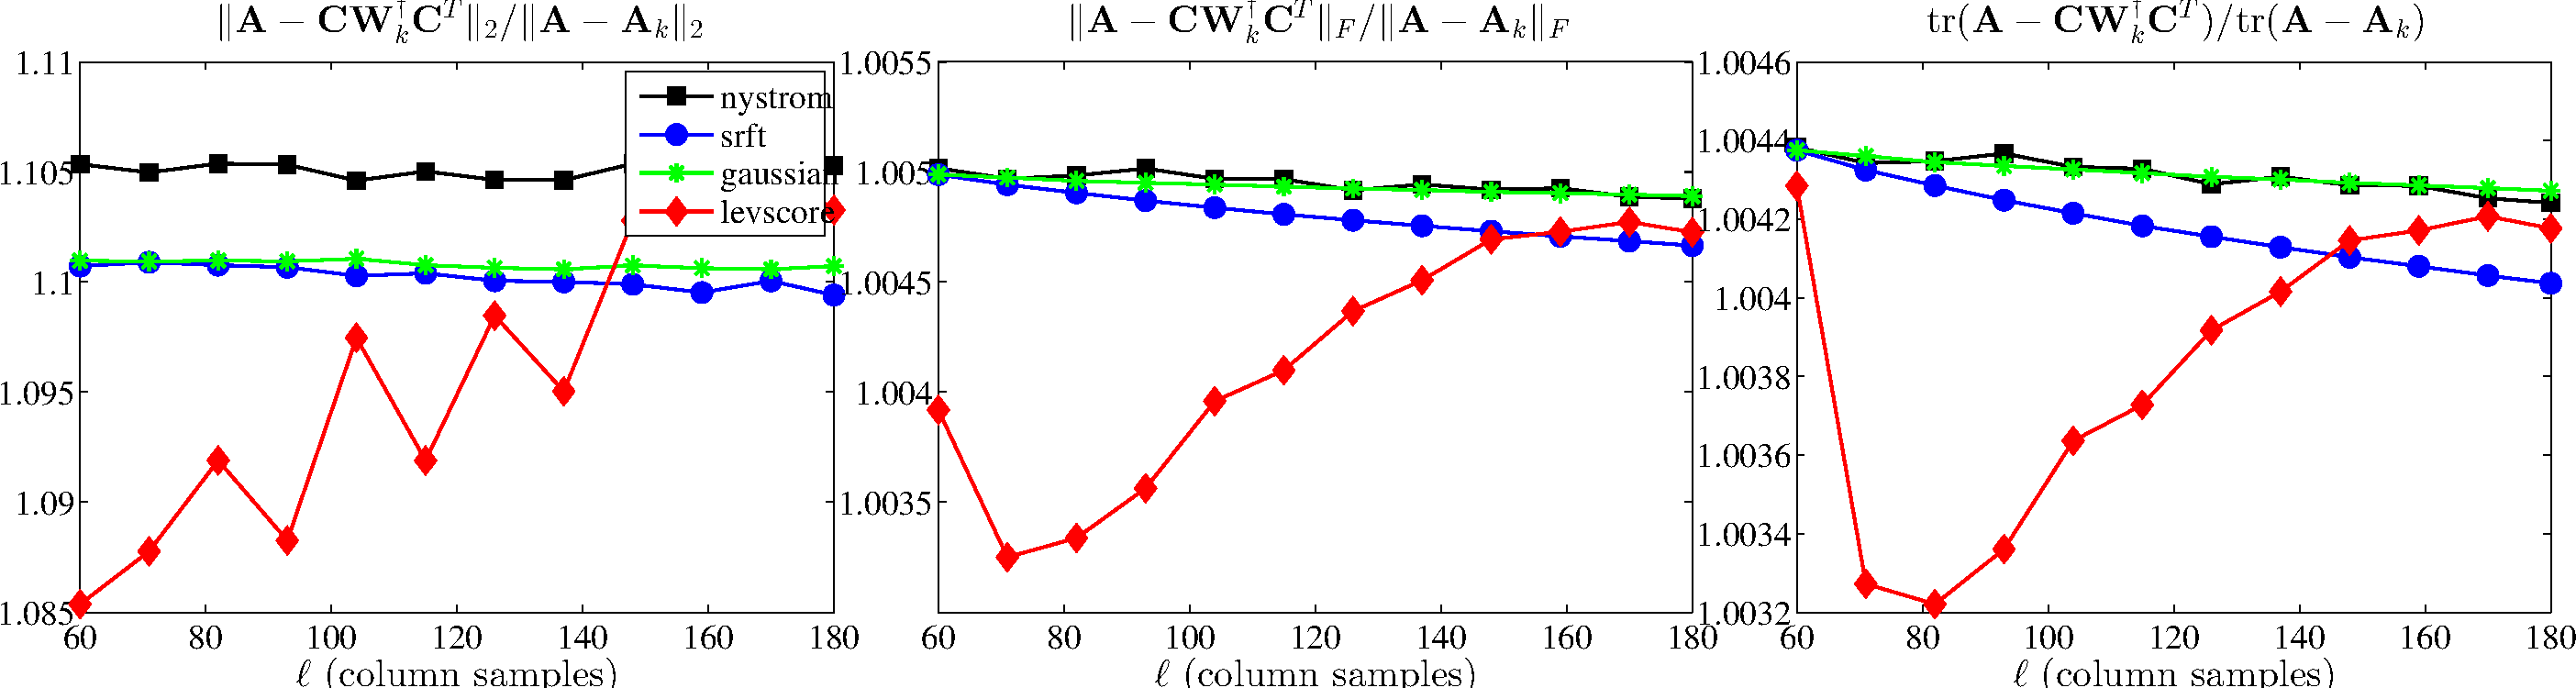
\includegraphics[width=6in, keepaspectratio=true]{figures/ch4/Gnutellarank60exact-methods-fixed-rank-errors}}
 \caption[Relative errors of rank-restricted SPSD sketches of the Enron and Gnutella Laplacian matrices]{%
 {\sc Relative errors of rank-restricted SPSD sketches of the Enron and Gnutella Laplacian matrices.}
 The relative spectral, Frobenius, and trace-norm errors~\eqref{ch4:eqn:relerr2} of several rank-restricted
 SPSD sketches, as a function of the number of columns samples $\ell$, 
 for the Enron and Gnutella Laplacian matrices, with two choices of the rank parameter $k$.}%
 \label{ch4:fig:laplacian-exact-errors-2b}
\end{figure}

Figures~\ref{ch4:fig:laplacian-exact-errors-1a}--\ref{ch4:fig:laplacian-exact-errors-2b} 
show the reconstruction error results for sampling and mixture methods 
applied to several normalized graph Laplacians.
Figures~\ref{ch4:fig:laplacian-exact-errors-1a} and~\ref{ch4:fig:laplacian-exact-errors-1b} 
show GR and HEP, each for two values of the rank parameter. The remaining two show
Enron and Gnutella, again each for two values of the 
rank parameter.
The first two figures show the ratios of the spectral, Frobenius, and trace-norm approximation 
errors of non-rank-restricted sketches to the optimal rank-$k$ 
approximation errors, as a function of the number of column samples~$\ell.$
The remaining two similarly show the errors of the rank-restricted sketches.

These and subsequent figures contain a lot of information, some of which is
peculiar to the given matrices and some of which is more general.
In light of subsequent discussion, several observations are worth making 
about the results presented in these figures.
\begin{itemize}
\item
All of the SPSD sketches provide quite accurate 
approximations even with only $k$ column samples (or 
in the case of the Gaussian and SRFT mixtures, with only $k$ linear 
combinations of vectors). 
Upon examination, this is partly due to the extreme sparsity and extremely 
slow spectral decay of these matrices which means, as shown in 
Table~\ref{ch4:table:datasets}, that only a small fraction of the (spectral or 
Frobenius or trace) mass is captured by the optimal rank $20$ or $60$ 
approximation. 
Thus although an SPSD sketch constructed from $20$ or $60$ vectors also only 
captures a small portion of the mass of the matrix, the relative error is 
small.  
\item
The scale of the vertical axes is different between different figures and 
subfigures.
This is to highlight properties within a given plot, but it can hide 
several things.
In particular, note that the scale for the spectral norm is generally
larger than for the Frobenius norm, which is generally larger than for the
trace norm, consistent with the size of those norms; and that the scale is 
larger for higher-rank approximations, e.g. compare GR $k=20$ with 
GR $k=60$, also consistent with the larger amount of mass captured by 
higher-rank approximations.
\item
Both the non-rank-restricted and rank-restricted results are the same for 
$\ell=k$.
For $\ell > k$, the non-rank-restricted errors tend to decrease (or 
at least not increase, as for GR and HEP the spectral norm error is flat as 
a function of $\ell$), which is intuitive.
While the rank-restricted errors also tend to decrease for $\ell > k$, 
the decrease is much less (since the rank-restricted plots are bounded below 
by unity) and the behavior is much more complicated as a function of 
increasing $\ell$.
\item
The horizontal axes range from $k$ to $9k$ for the $k=20$ plots and to $3k$ for the 
$k=60$ plots.
As a practical matter, choosing $\ell$ between $k$ and (say) $2k$ or $3k$ is 
probably of greatest interest.
In this regime, there is an interesting tradeoff for the non-rank-restricted
plots: for moderately large values of $\ell$ in this regime, the error for 
leverage-based sampling is moderately better than for uniform sampling or 
random mixtures, while if one chooses $\ell$ to be much larger then the 
improvements from leverage-based sampling saturate and the uniform sampling 
and random mixture methods are better.
This is most obvious in the Frobenius-norm plots, although it is also seen in
the trace norm plots, and it suggests that some combination of leverage-based
sampling and uniform sampling might be best.
\item
For the rank-restricted plots, in some cases, e.g., with GR and HEP, 
the errors for leverage-based sampling are much better than for the other 
methods and quickly improve with increasing $\ell$ until they saturate; 
while in other cases, e.g., with Enron and Gnutella, the errors for
leverage-based sampling improve quickly and then degrade with increasing 
$\ell$.
Upon examination, the former phenomenon is similar to what was observed in 
the non-rank-restricted case and is due to the strong ``bias'' provided by 
the leverage score importance sampling distribution to the top part of the 
spectrum, allowing the sampling process to focus very quickly on the 
low-rank part of the input matrix.
(In some cases, this is due to the fact that the heterogeneity of 
the leverage score importance sampling distribution means that one is likely 
to choose the same high leverage columns multiple times, rather than 
increasing the accuracy of the extension by adding new columns whose 
leverage scores are lower.) 
The latter phenomenon of degrading error quality as $\ell$ is increased is 
more complex and seems to be due to some sort of ``overfitting'' caused by 
this strong bias and by choosing many more than $k$ columns.  
%% Although we do not completely undersand it, this phenomenon is seen in 
%% several of the examples below.
\item
The behavior of the approximations with respect to the spectral norm is 
quite different from the behavior in the Frobenius and trace norms. 
In the latter, as the number of samples $\ell$ increases, the errors tend to 
decrease, although in an erratic manner for some of the rank-restricted 
plots; while for the former, the errors tend to be much flatter as a function 
of increasing $\ell$ for at least the Gaussian, SRFT, and uniformly column sampled (i.e., Nystr\"om)
sketches.
\end{itemize}
All in all, there seems to be quite complicated behavior for low-rank 
sketches for these Laplacian matrices.
Several of these observations can also be made for subsequent figures; but
in some other cases the (very sparse and not very low rank) structural 
properties of the data are primarily responsible.

\subsubsection{Linear kernels}

\begin{figure}[htp]
 \centering
 \subfigure[Dexter, $k = 8$]{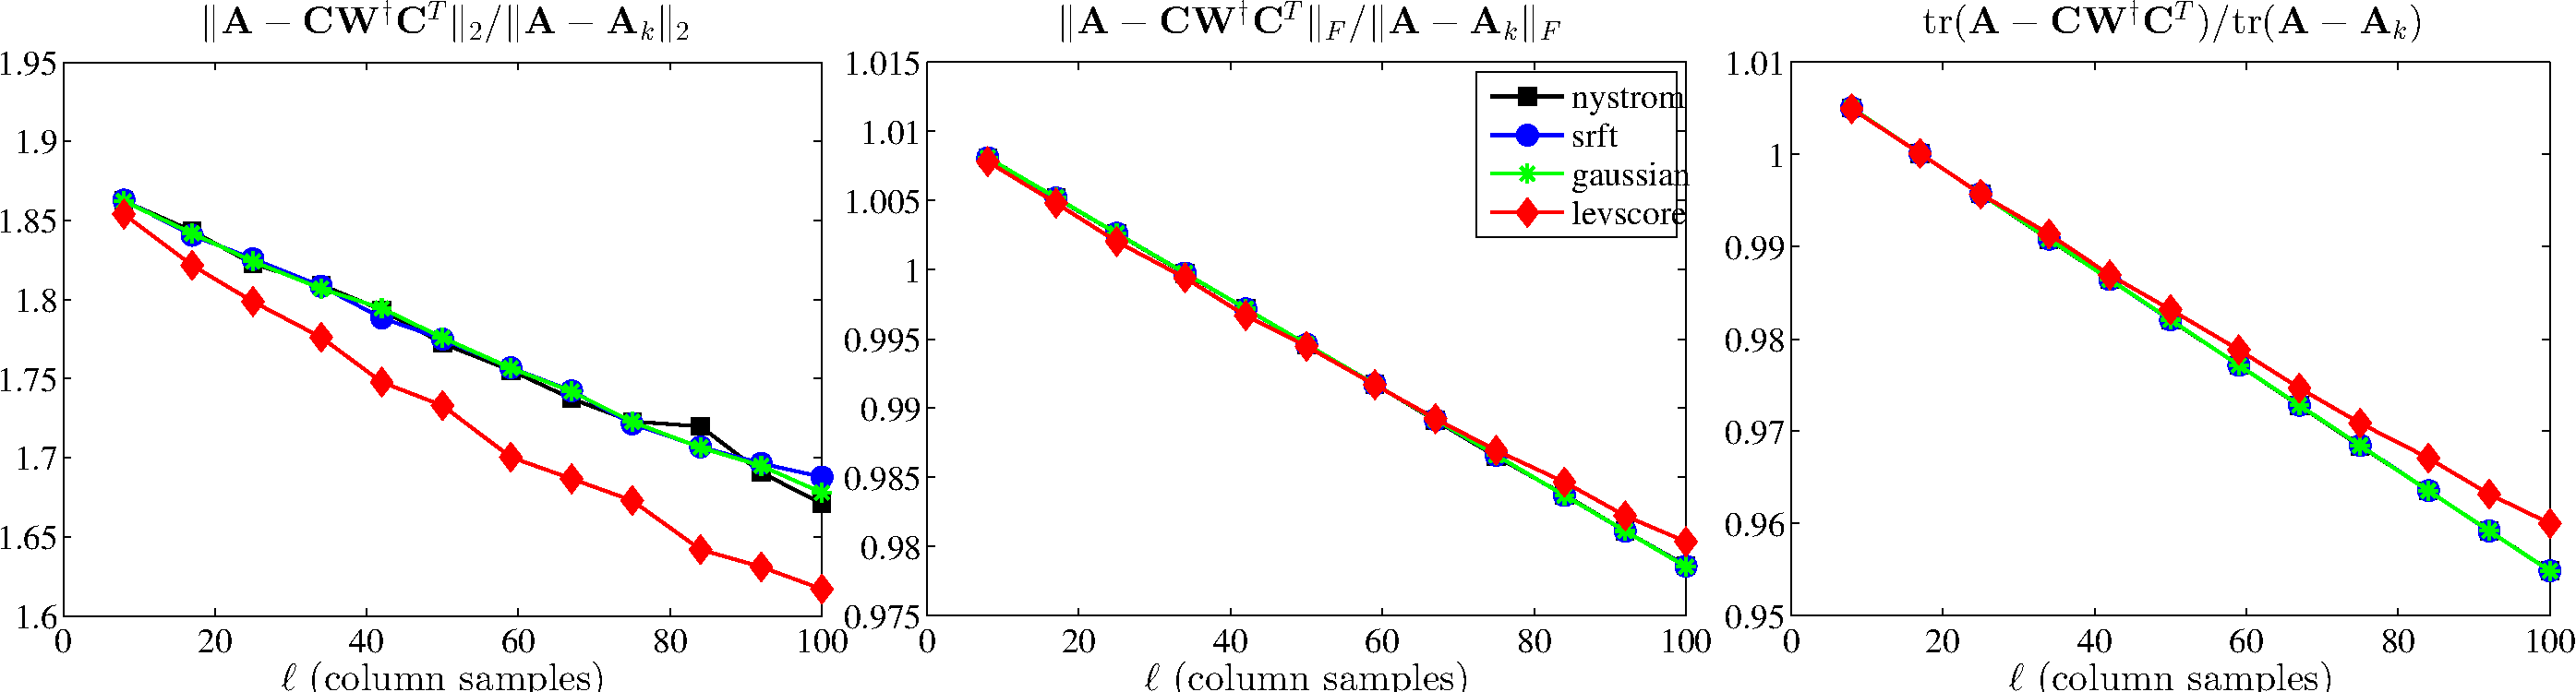
\includegraphics[width=6in, keepaspectratio=true]{figures/ch4/Dexterrank8exact-methods-nonfixed-rank-errors}}
 
 \subfigure[Protein, $k = 10$]{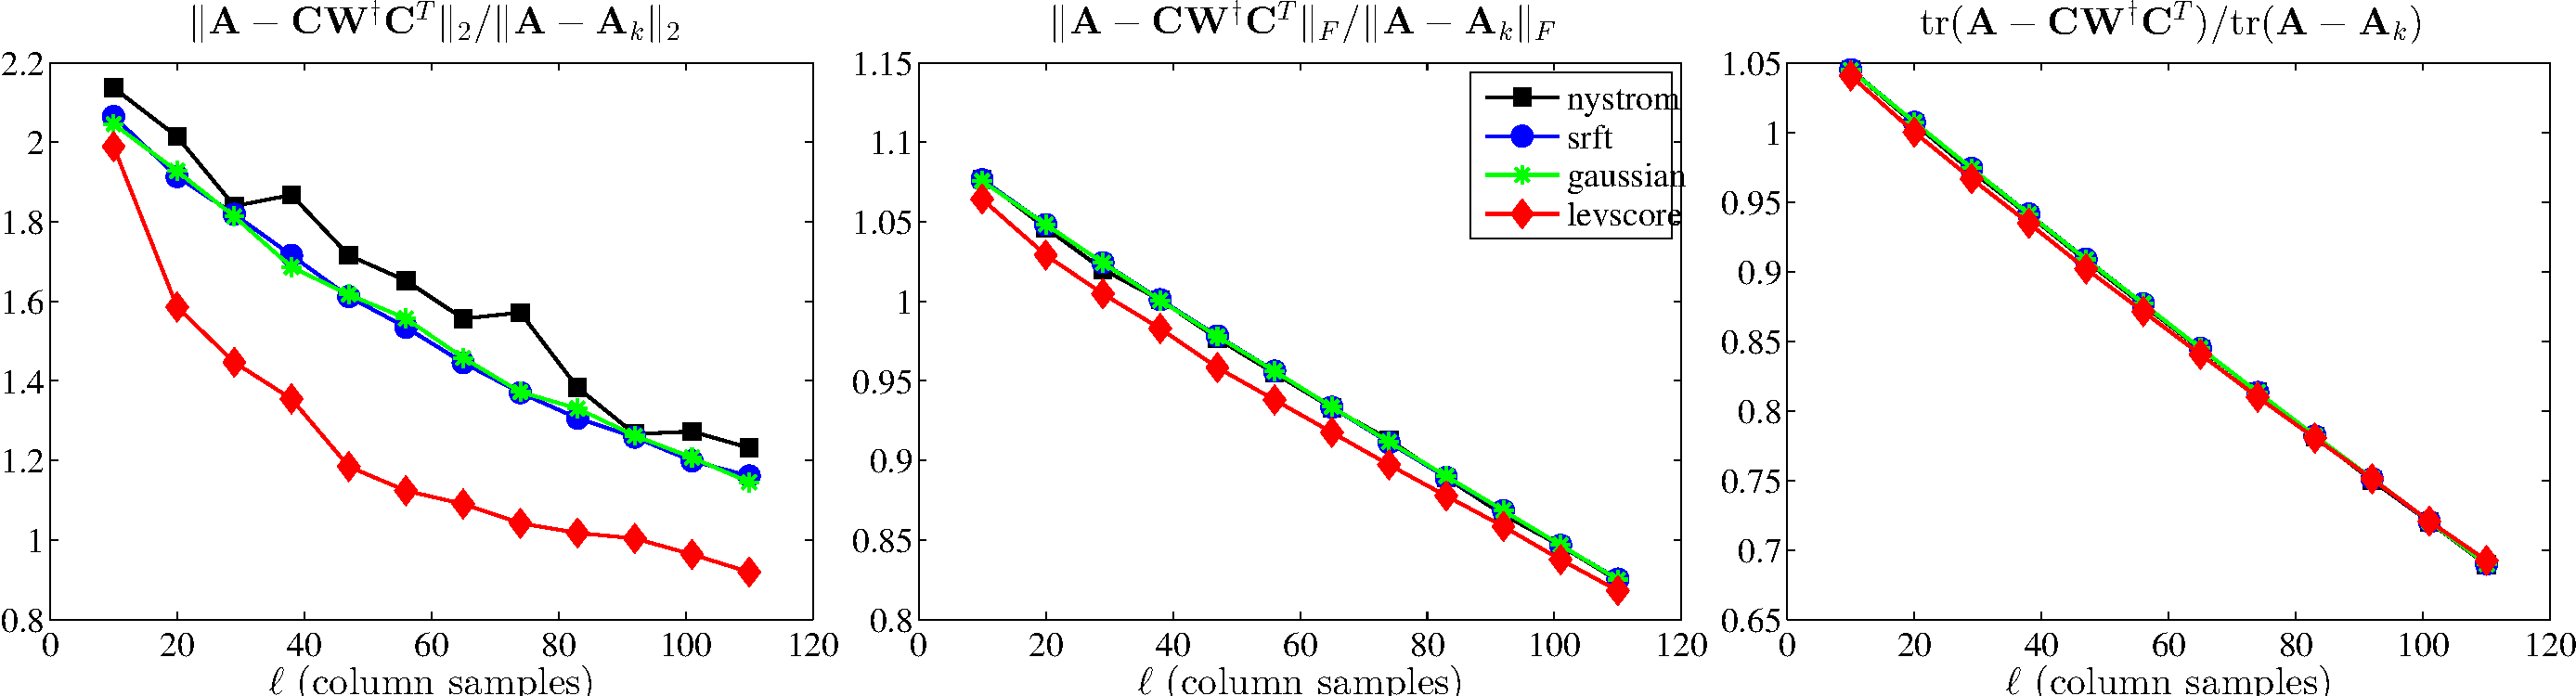
\includegraphics[width=6in, keepaspectratio=true]{figures/ch4/Proteinrank10exact-methods-nonfixed-rank-errors}}
 
 \subfigure[SNPs, $k = 5$]{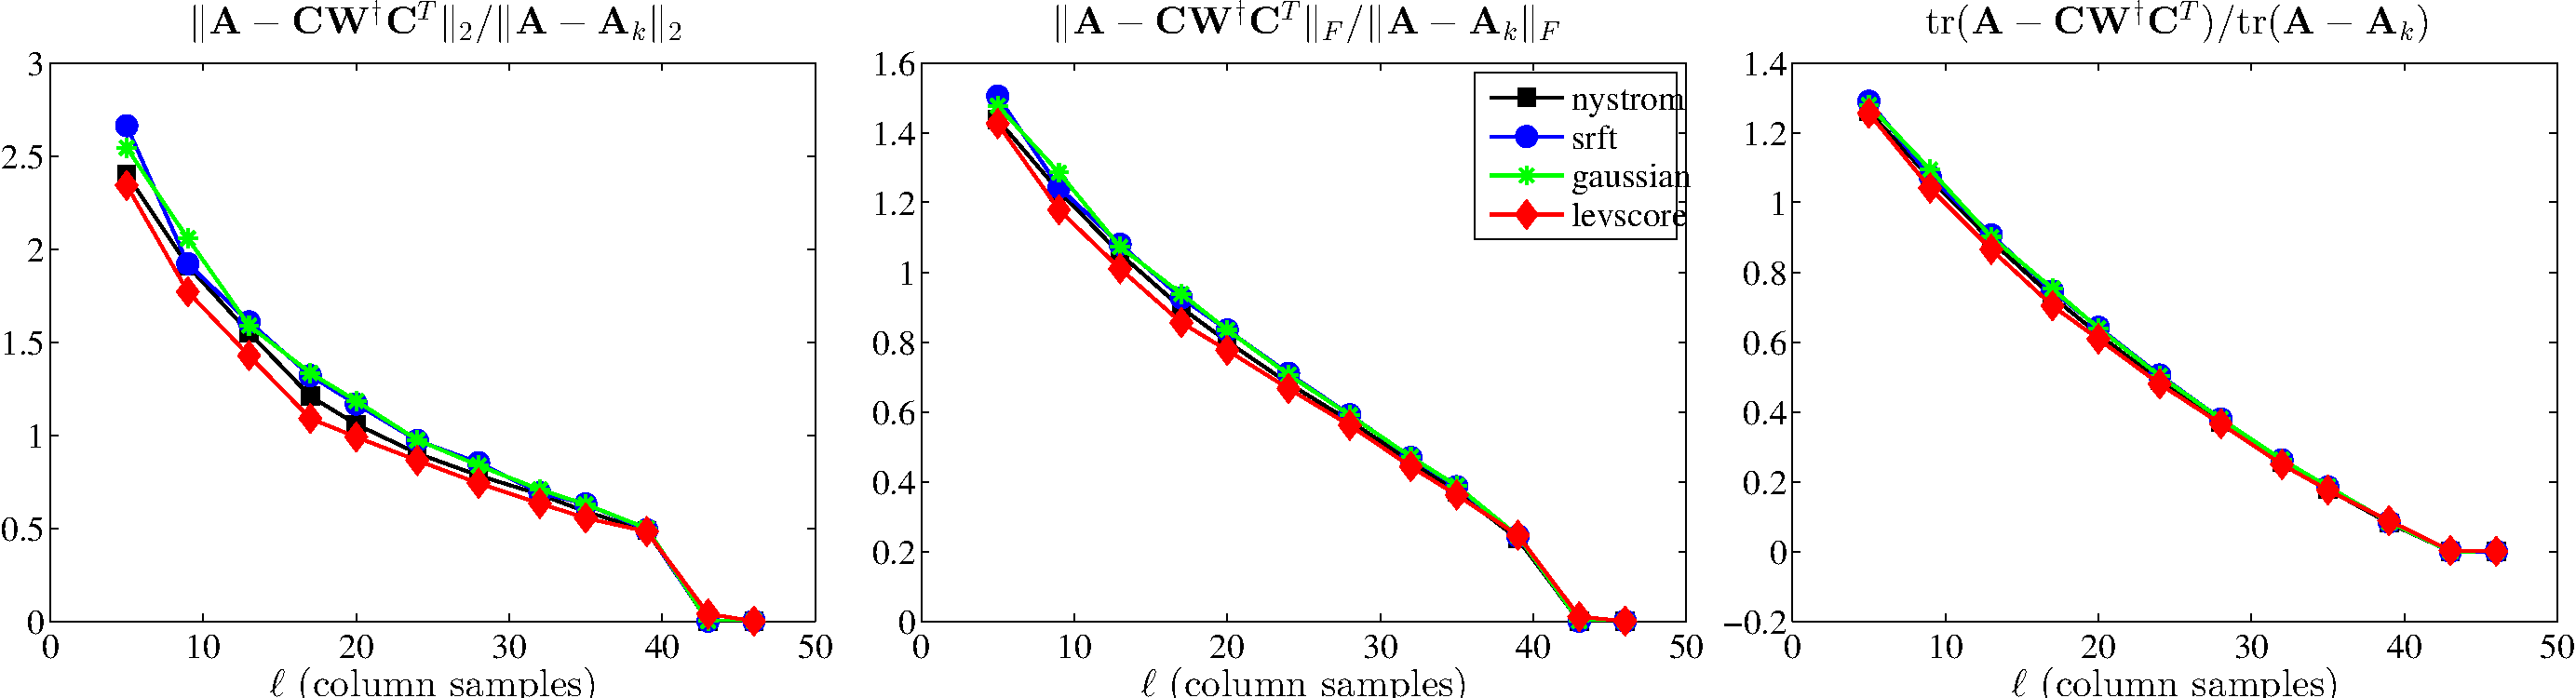
\includegraphics[width=6in, keepaspectratio=true]{figures/ch4/SNPSrank5exact-methods-nonfixed-rank-errors}}
 
 \subfigure[Gisette, $k = 12$]{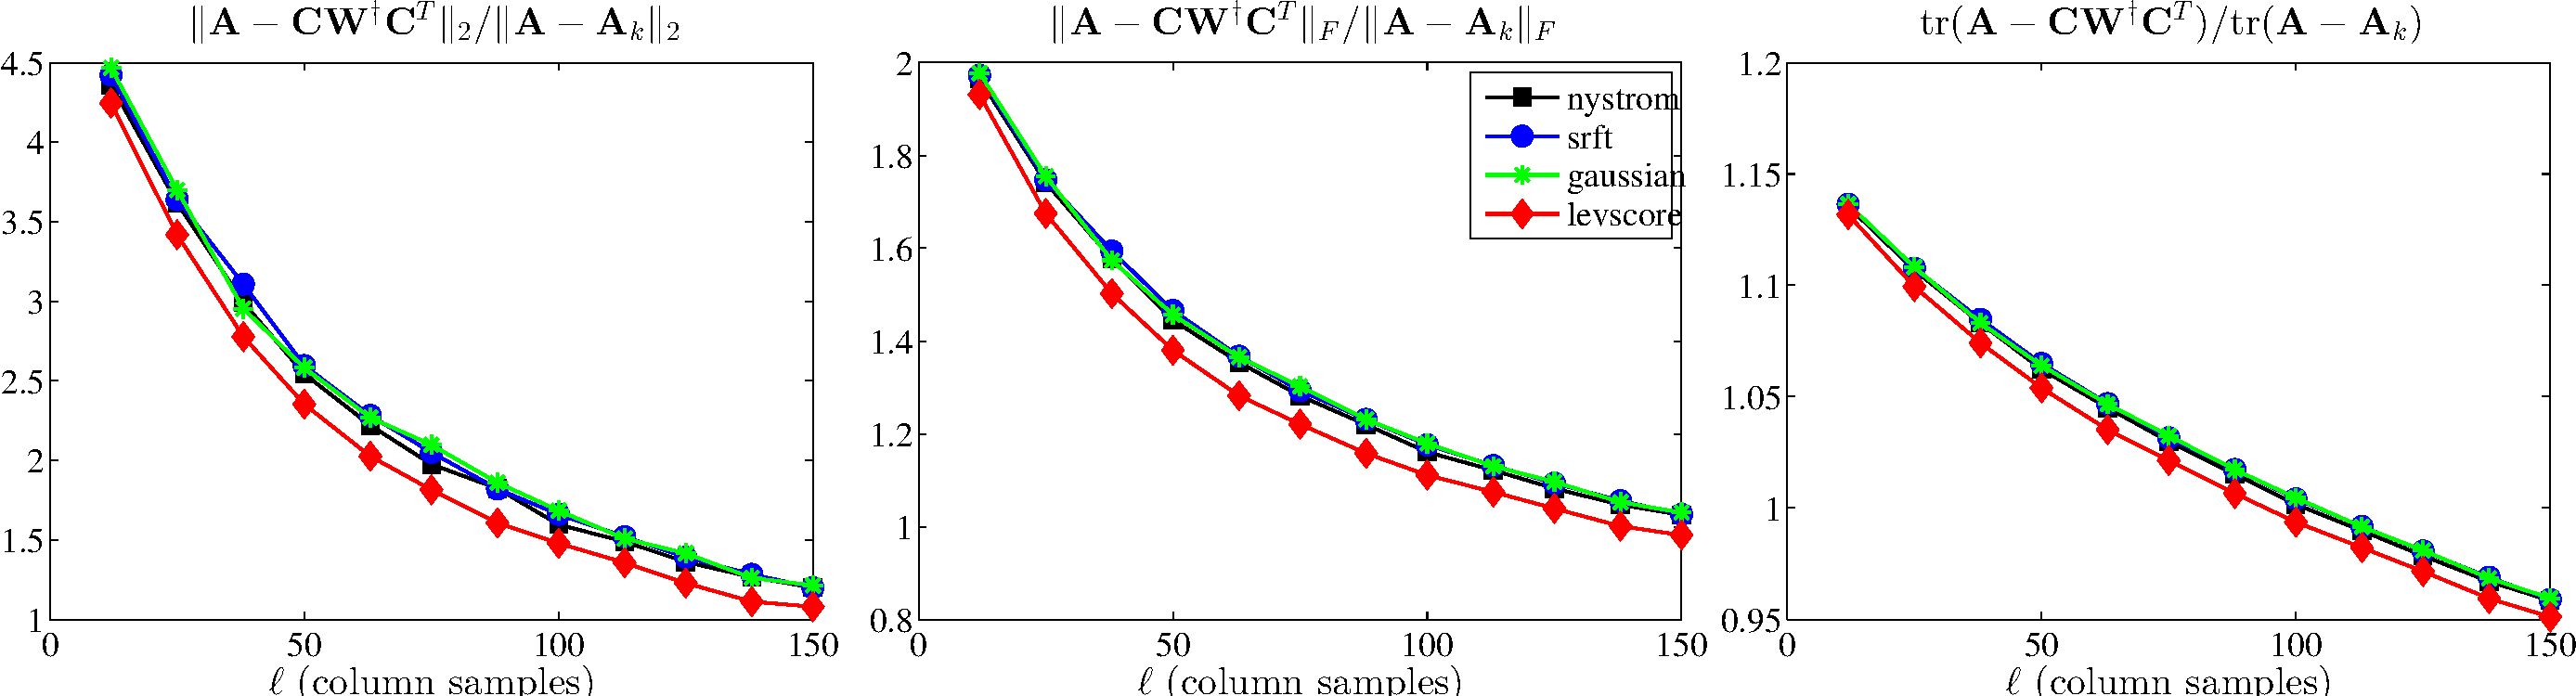
\includegraphics[width=6in, keepaspectratio=true]{figures/ch4/Gisetterank12exact-methods-nonfixed-rank-errors}}
 \caption[Relative errors of non-rank-restricted SPSD sketches of the linear kernel matrices]{%
 {\sc Relative errors of non-rank-restricted SPSD sketches of the linear kernel matrices.}
 The relative spectral, Frobenius, and trace-norm errors~\eqref{ch4:eqn:relerr1} of several non-rank-restricted
 SPSD sketches, as a function of the number of columns samples $\ell$, 
 for the linear kernel matrices.}%
 \label{ch4:fig:linearkernel-exact-errors-a}
\end{figure}

\begin{figure}[htp]
 \centering
 \subfigure[Dexter, $k = 8$]{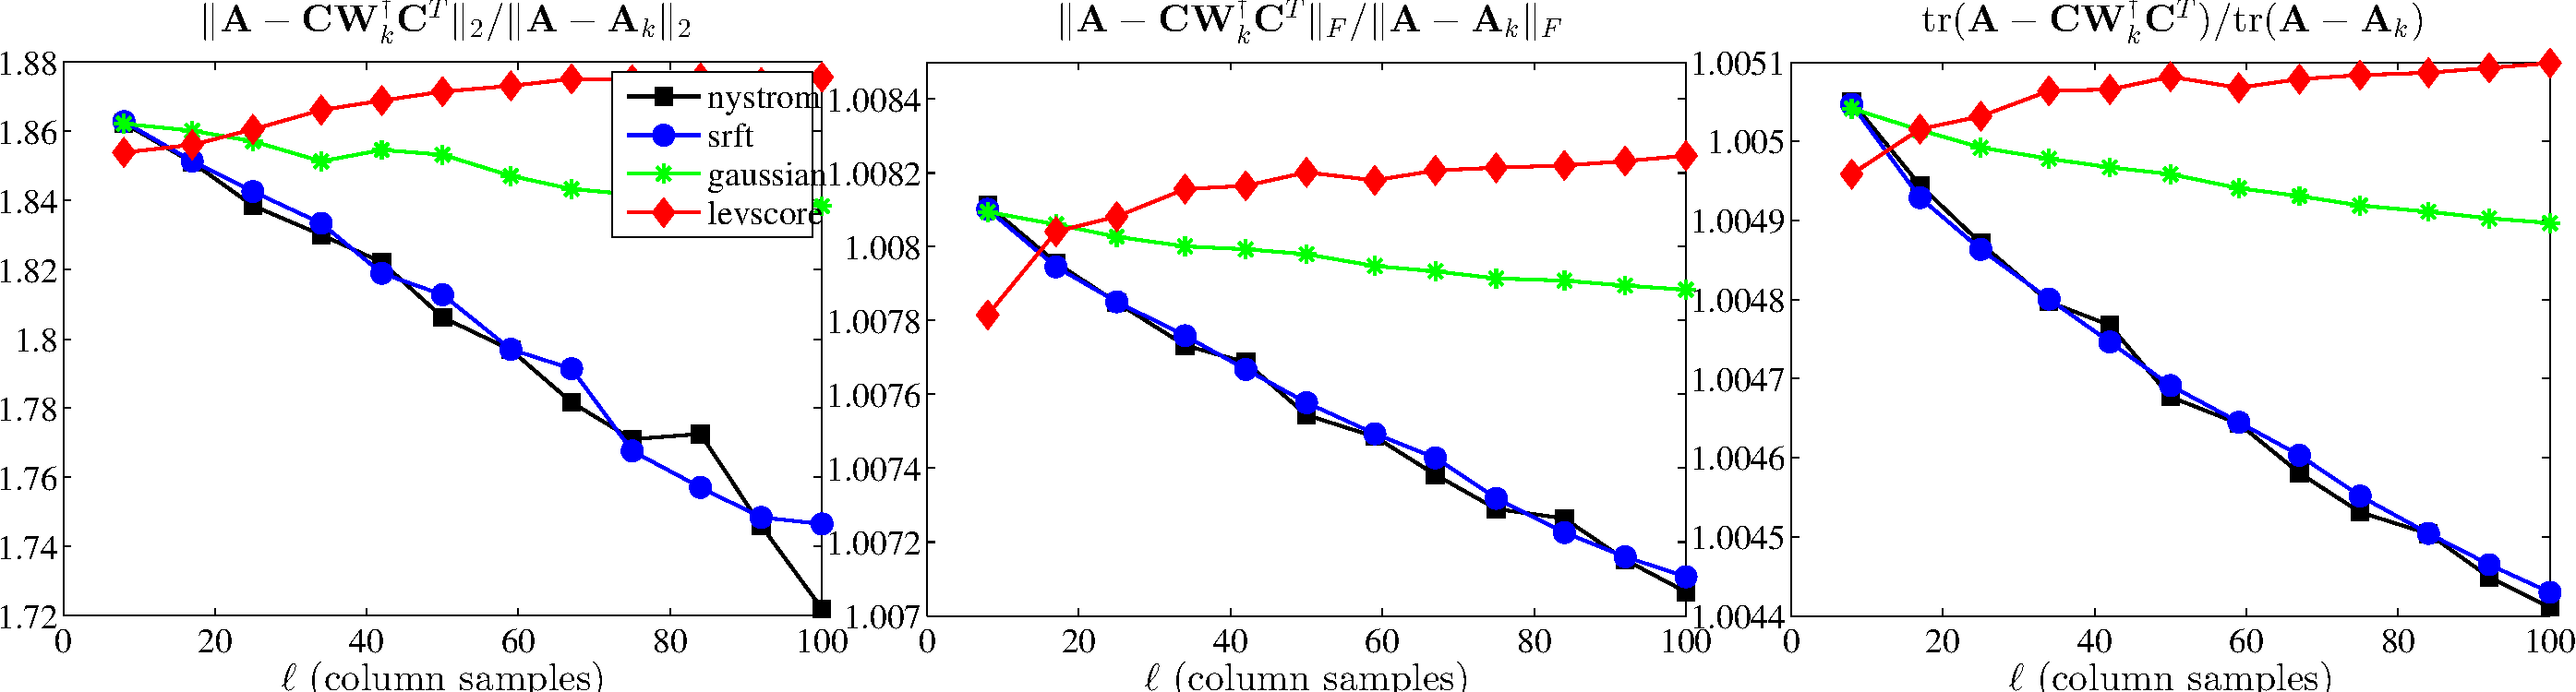
\includegraphics[width=6in, keepaspectratio=true]{figures/ch4/Dexterrank8exact-methods-fixed-rank-errors}}
 
 \subfigure[Protein, $k = 10$]{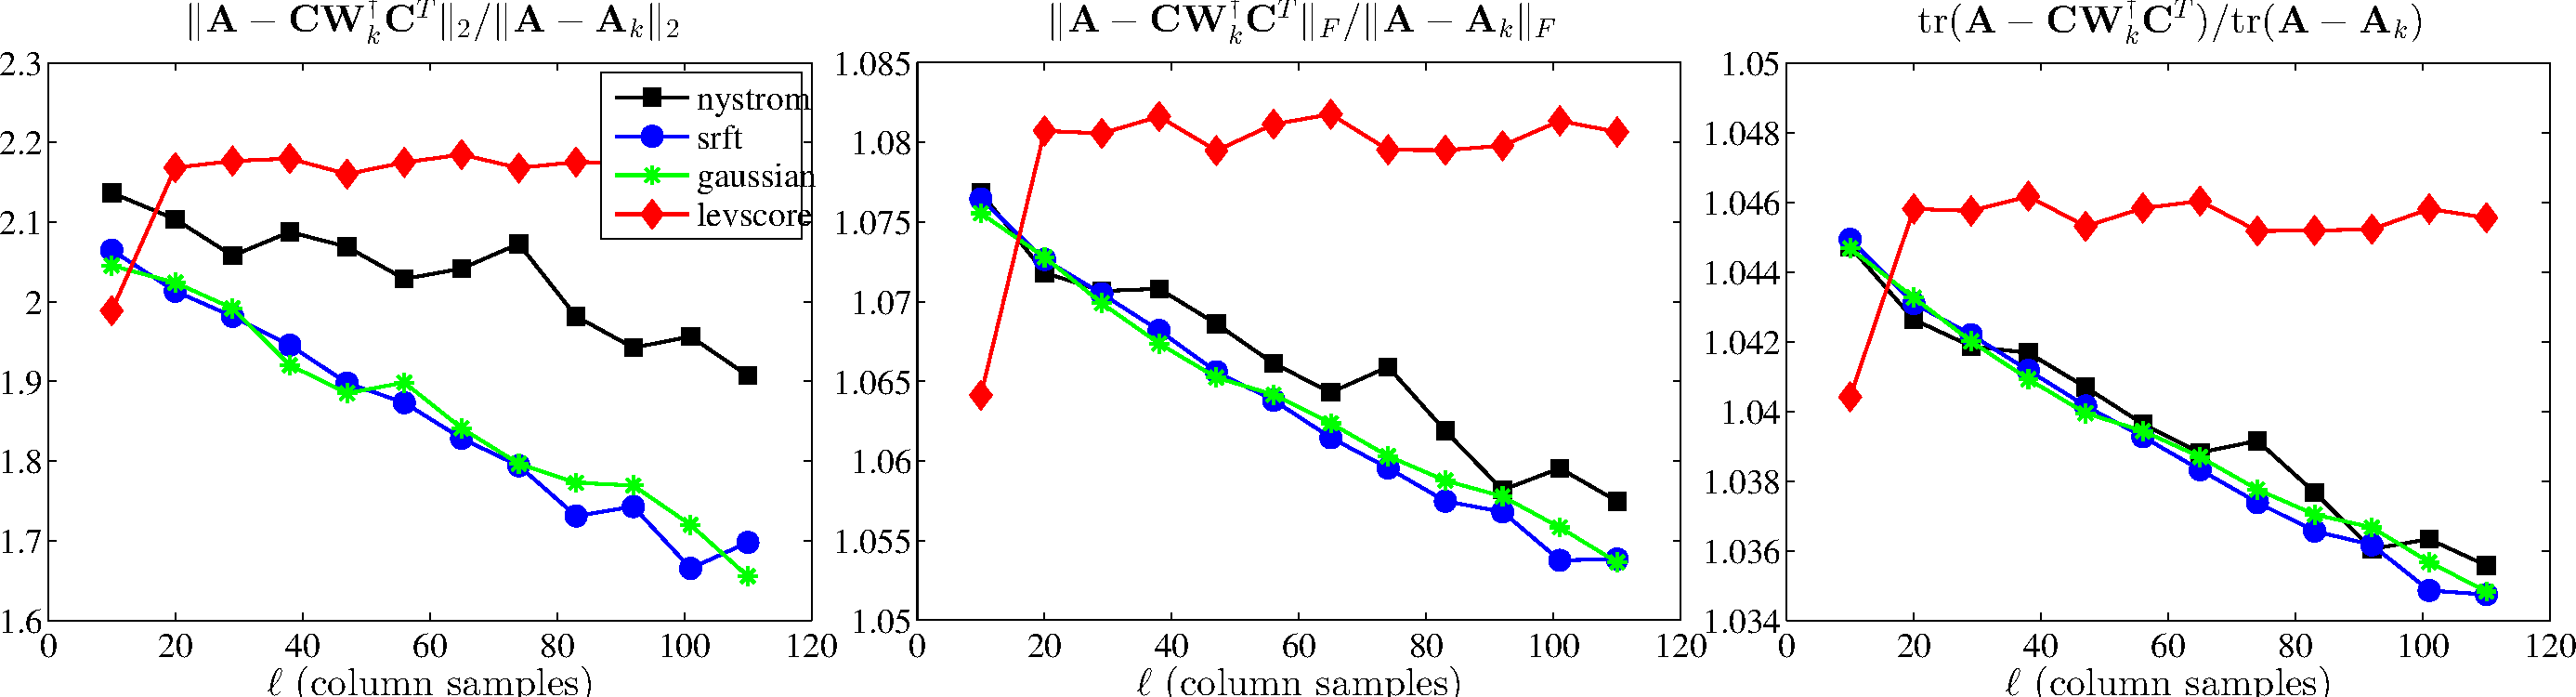
\includegraphics[width=6in, keepaspectratio=true]{figures/ch4/Proteinrank10exact-methods-fixed-rank-errors}}
 
 \subfigure[SNPs, $k = 5$]{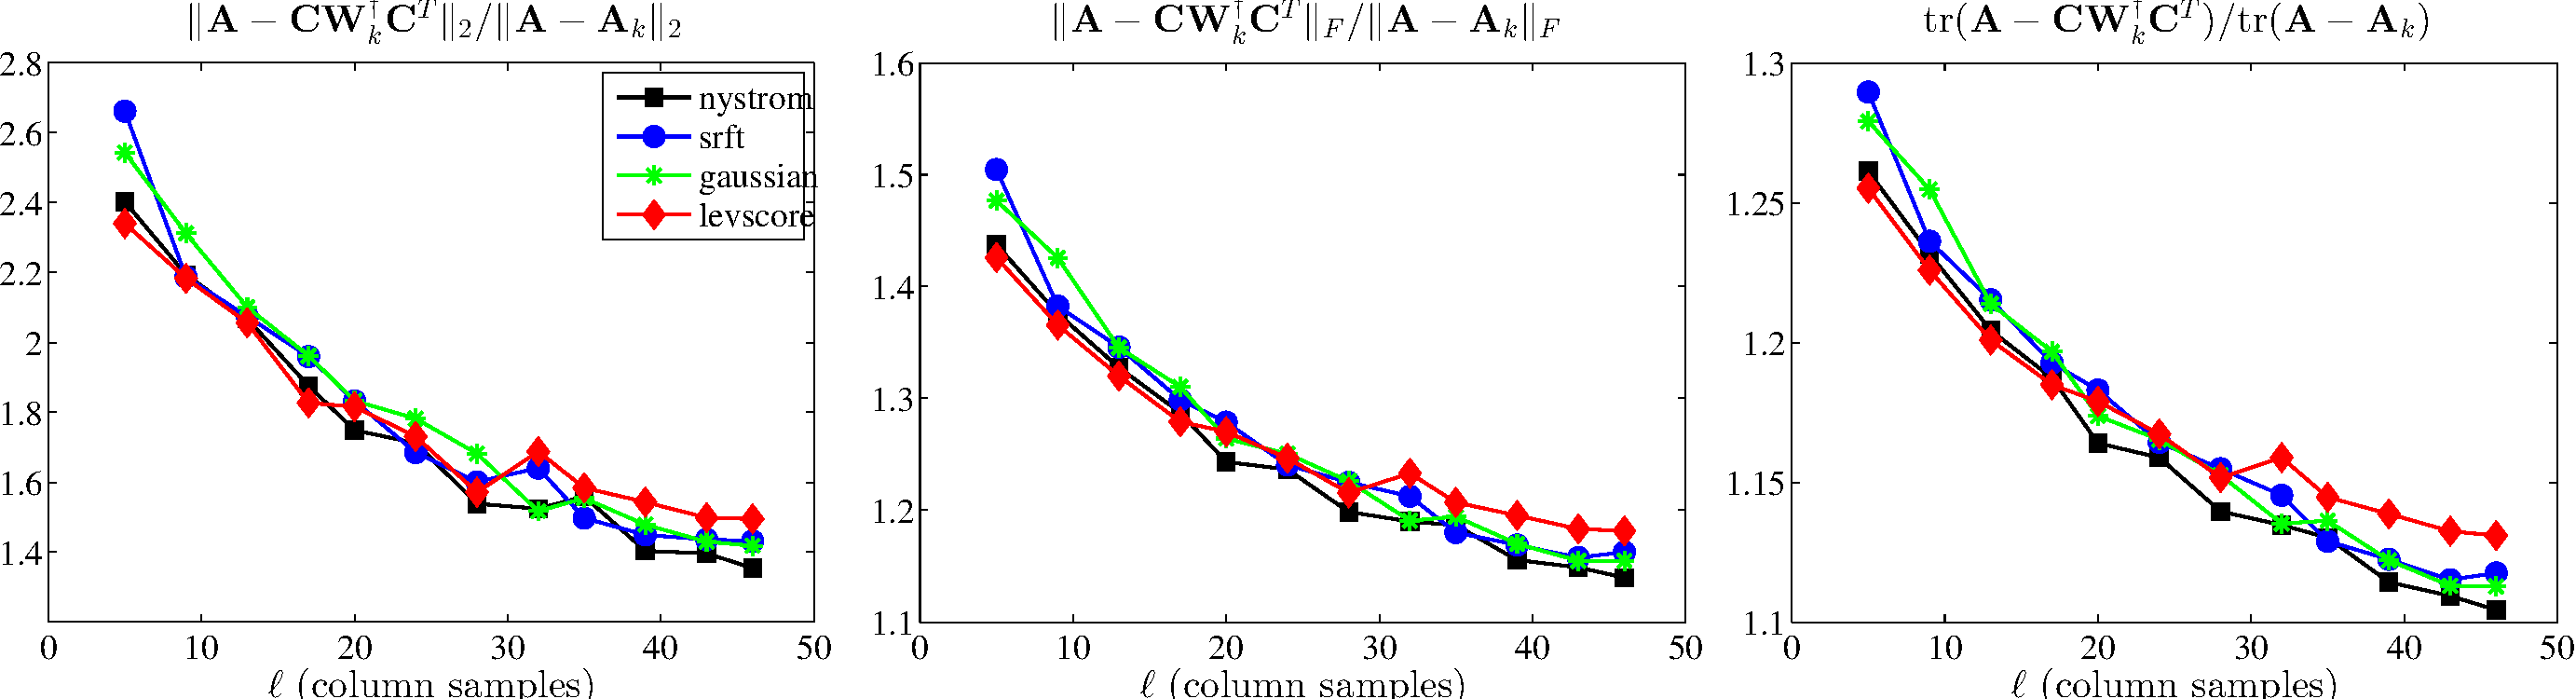
\includegraphics[width=6in, keepaspectratio=true]{figures/ch4/SNPSrank5exact-methods-fixed-rank-errors}}
 
 \subfigure[Gisette, $k = 12$]{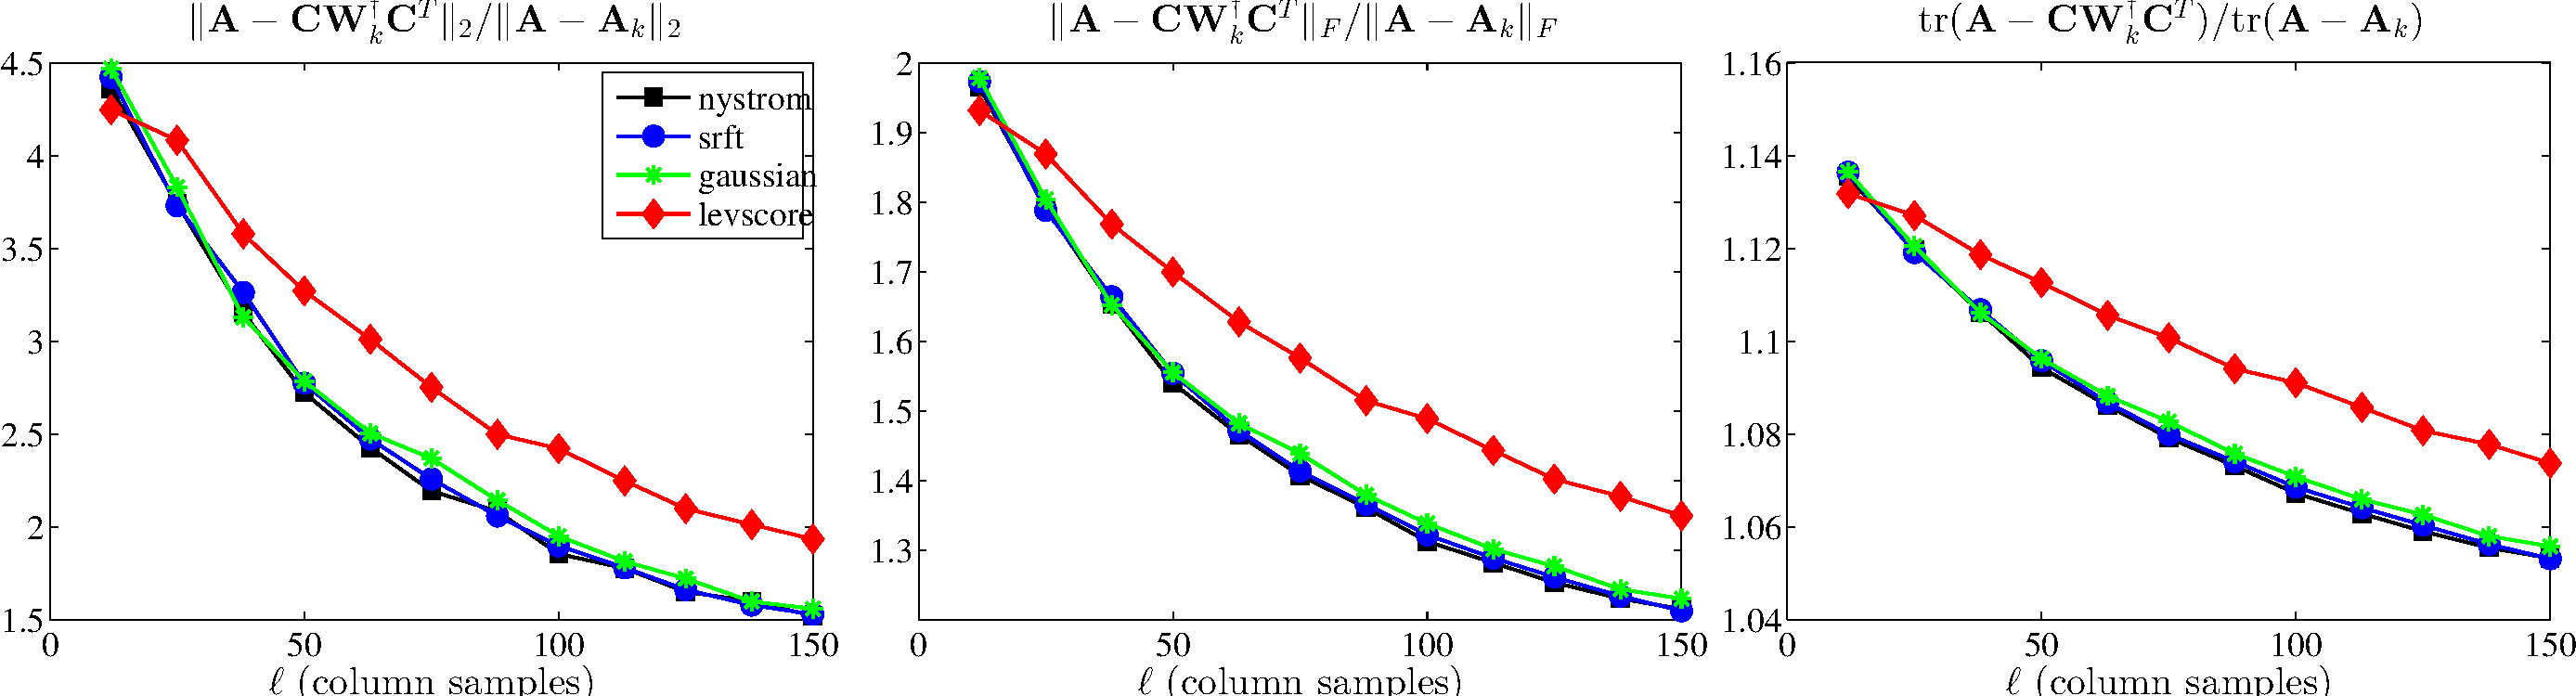
\includegraphics[width=6in, keepaspectratio=true]{figures/ch4/Gisetterank12exact-methods-fixed-rank-errors}}
 \caption[Relative errors of rank-restricted SPSD sketches of the linear kernel matrices]{%
 {\sc Relative errors of rank-restricted SPSD sketches of the linear kernel matrices.}
 The relative spectral, Frobenius, and trace-norm errors~\eqref{ch4:eqn:relerr2} of several rank-restricted
 SPSD sketches, as a function of the number of columns samples $\ell$, 
 for the linear kernel matrices. }%
 \label{ch4:fig:linearkernel-exact-errors-b}
\end{figure}

Figures~\ref{ch4:fig:linearkernel-exact-errors-a} and~\ref{ch4:fig:linearkernel-exact-errors-b}
show the reconstruction error results for sampling and mixture methods 
applied to several linear kernels.  
The matrices (Dexter, Protein, SNPs, and Gisette) are all quite low-rank 
and have fairly uniform leverage scores.
Several observations are worth making about the results presented in these 
figures.
\begin{itemize}
\item
All of the methods perform quite similarly for the non-rank-restricted 
case: all have errors that decrease smoothly with increasing $\ell$, and in 
this case there is little advantage to using methods other than uniform 
sampling (since they perform similarly and are more expensive).
Also, since the ranks are so low and the leverage scores are so uniform, the 
leverage score extension is no longer significantly distinguished by its 
tendency to saturate quickly.
\item
The scale of the vertical axes is much larger than for the Laplacian matrices,
mostly since the matrices are much better approximated by low-rank 
matrices, although the scale decreases as one goes from spectral to 
Frobenius to trace reconstruction error, as before.
\item
For SNPs and Gisette, the rank-restricted reconstruction results are 
very similar for all four methods, with a smooth decrease in error as
$\ell$ is increased, although interestingly using leverage scores is
slightly worse for Gisette.
For Dexter and Protein, the situation is more complicated: using the SRFT 
always leads to smooth decrease as $\ell$ is increased, and uniform sampling
generally behaves the same way also; Gaussian mixtures behave this way 
for Protein, but 
for Dexter Gaussian mixtures are noticably worse than SRFT and uniform 
sampling; and, except for very small values of $\ell$, leverage-based 
sampling is worse still and gets noticably worse as $\ell$ is increased.
Even this poor behavior of leverage score sampling on the linear kernels is 
notably worse than for the rank-restricted Laplacians, where there was a 
range of moderately small $\ell$ where leverage score sampling was much 
superior to other methods.
\end{itemize}
These linear kernels (and also to some extent the dense RBF kernels below
that have larger $\sigma$ parameter) are examples of relatively ``nice'' 
machine learning matrices that are similar to matrices where uniform 
sampling has been shown to perform well 
previously~\cite{TKR08,KMT09a,KMT09,KMT12}; and for these matrices our 
empirical results agree with these prior works.


\subsubsection{Dense and sparse RBF kernels}

\begin{figure}[htp]
 \centering
 \subfigure[AbaloneD, $\sigma = .15, k = 20$]{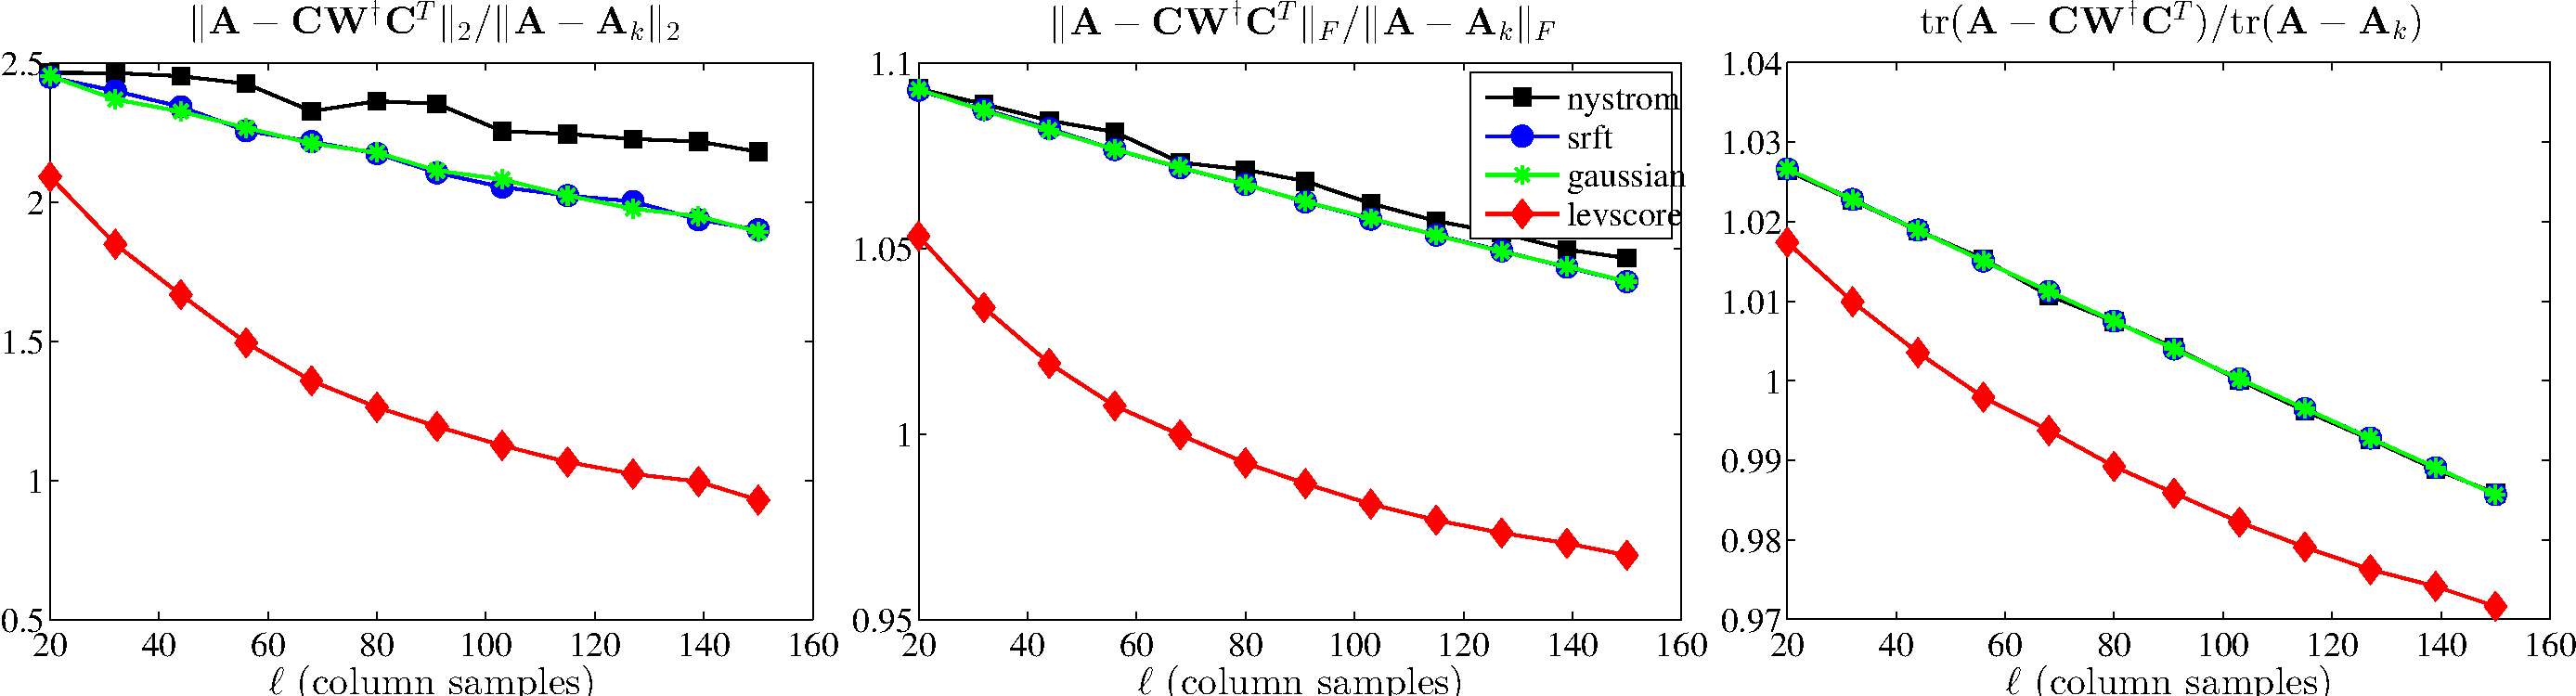
\includegraphics[width=6in, keepaspectratio=true]{figures/ch4/Abalonesigmapt15exact-methods-nonfixed-rank-errors}}
 
 \subfigure[AbaloneD, $\sigma = 1, k = 20$]{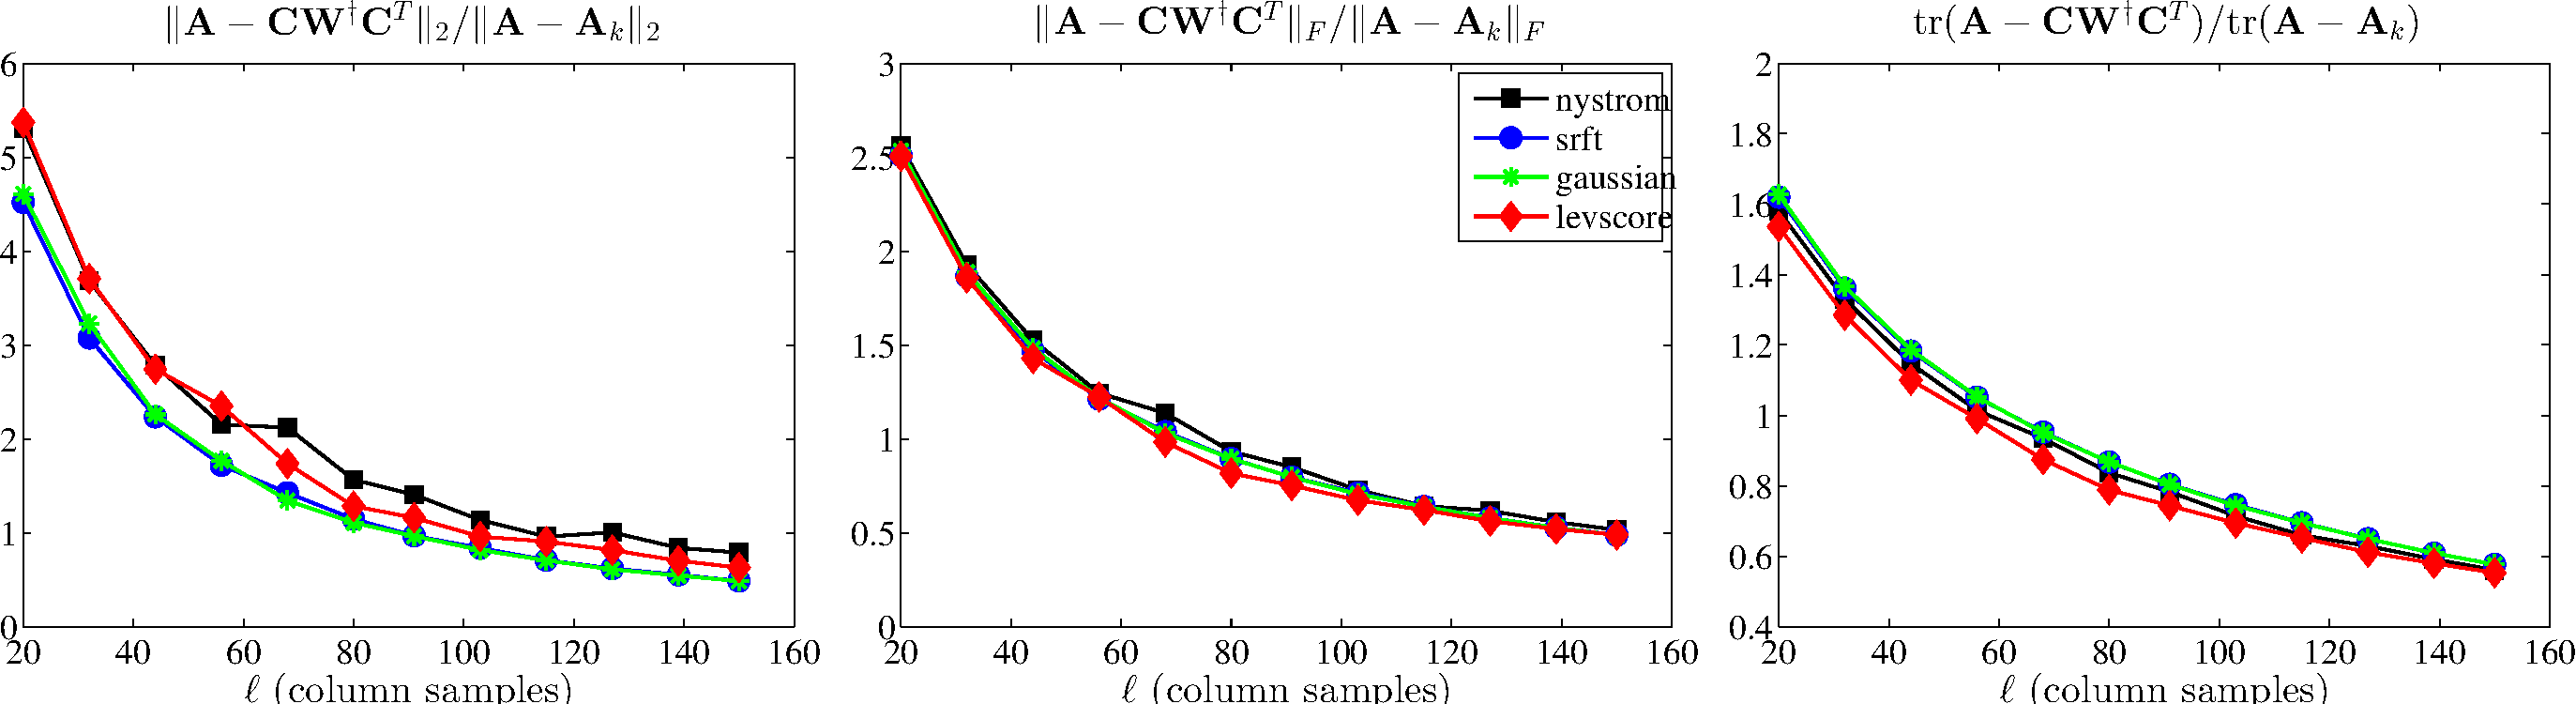
\includegraphics[width=6in, keepaspectratio=true]{figures/ch4/Abalonesigma1exact-methods-nonfixed-rank-errors}}
 
 \subfigure[WineD, $\sigma = 1, k = 20$]{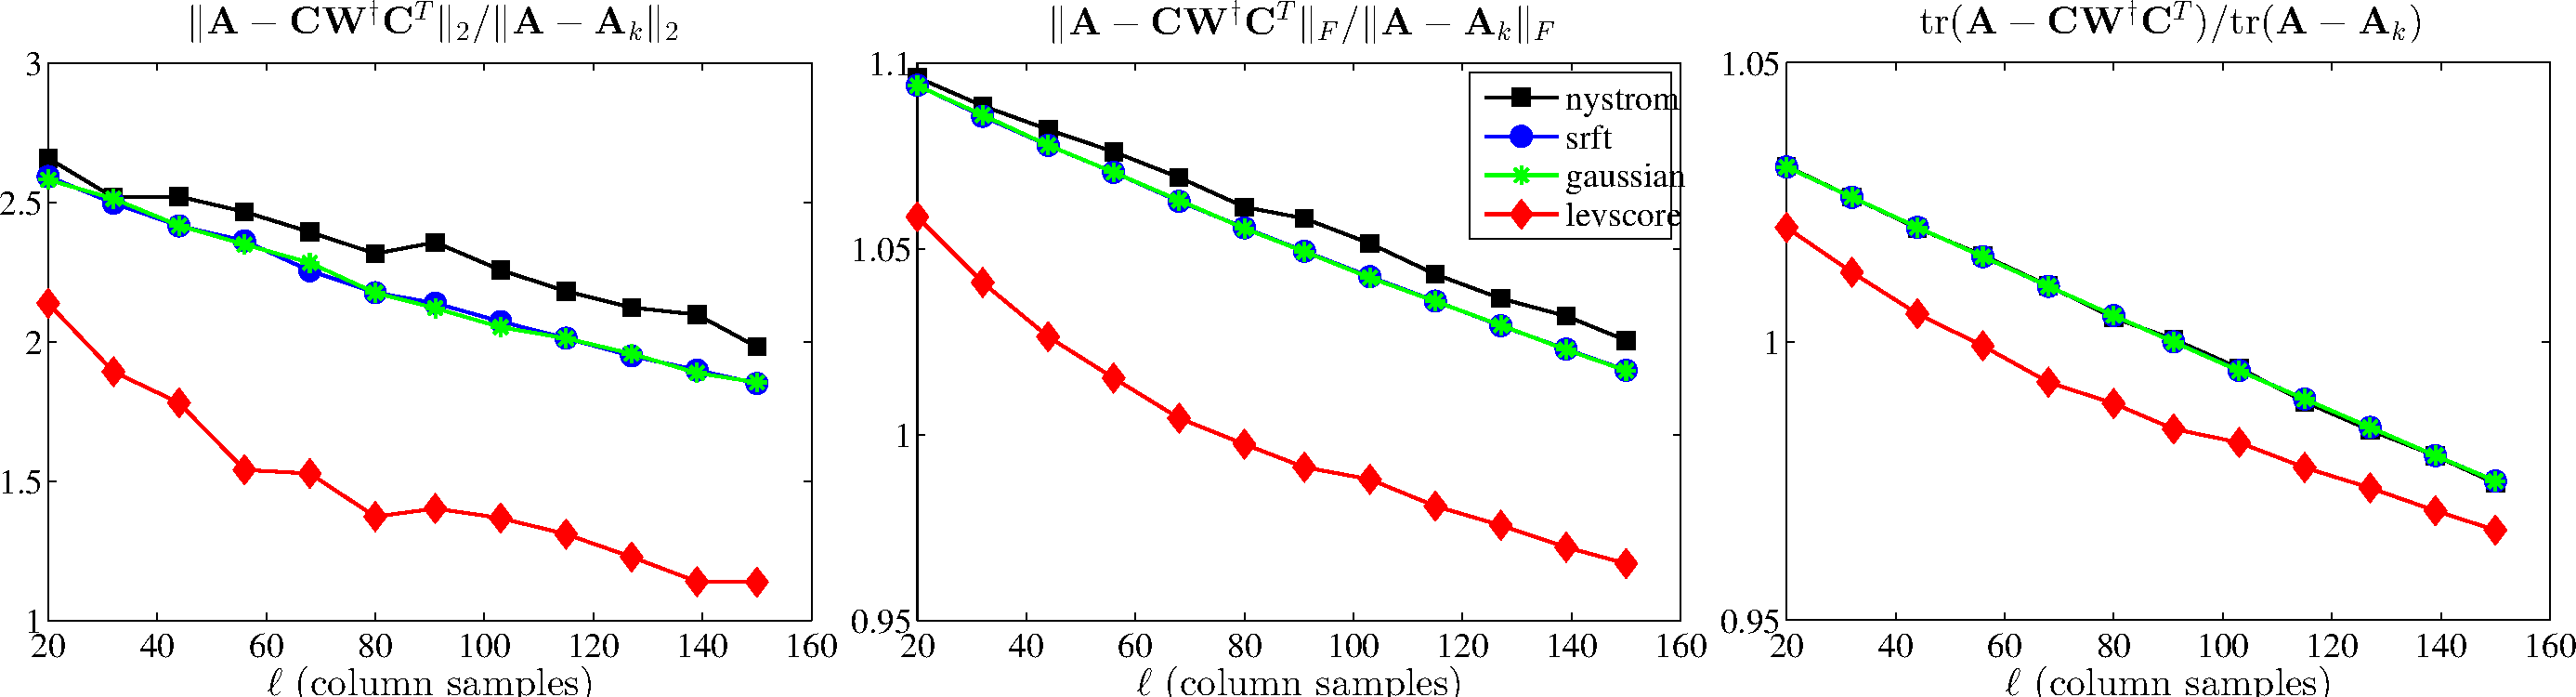
\includegraphics[width=6in, keepaspectratio=true]{figures/ch4/Winesigma1exact-methods-nonfixed-rank-errors}}
 
 \subfigure[WineD, $\sigma = 2.1, k = 20$]{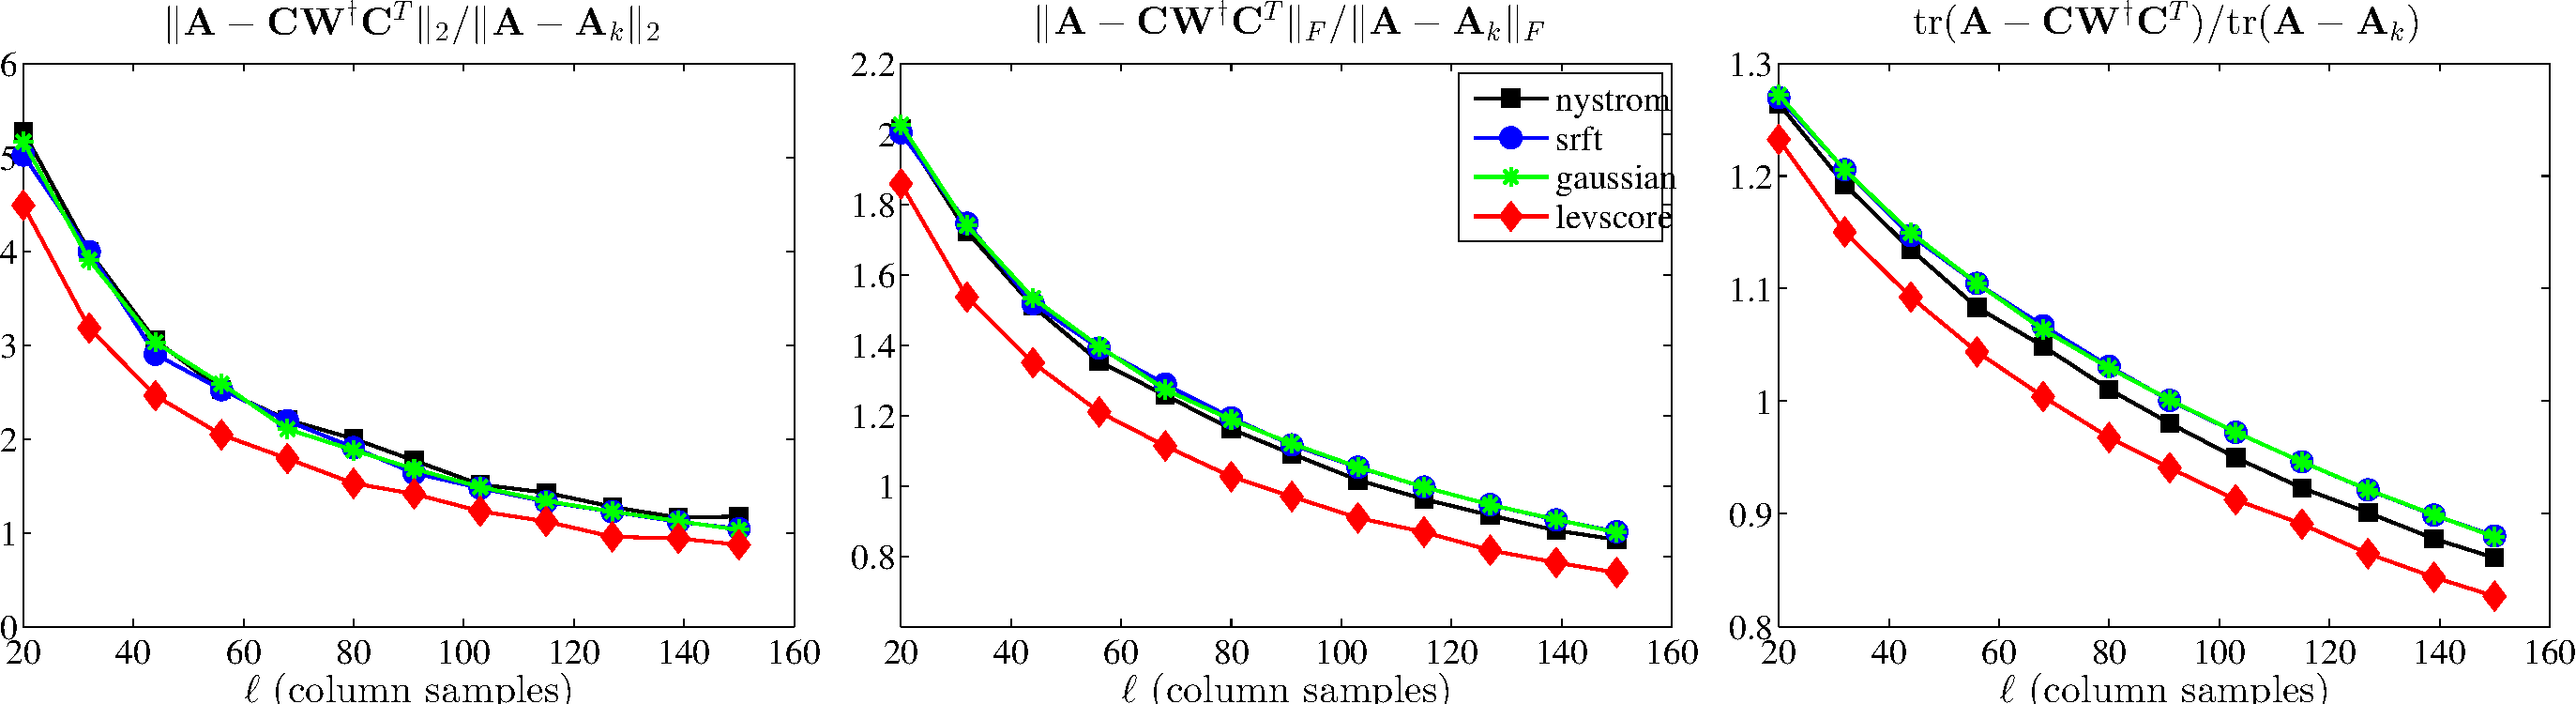
\includegraphics[width=6in, keepaspectratio=true]{figures/ch4/Winesigma2pt1exact-methods-nonfixed-rank-errors}}
 \caption[Relative errors of non-rank-restricted SPSD sketches of the dense RBFK matrices]{%
 {\sc Relative errors of non-rank-restricted SPSD sketches of the dense RBFK matrices.}
 The relative spectral, Frobenius, and trace-norm errors~\eqref{ch4:eqn:relerr1} of several non-rank-restricted
 SPSD sketches, as a function of the number of columns samples $\ell$, 
 for the dense RBFK matrices. }%
 \label{ch4:fig:denserbf-exact-errors-a}
\end{figure}

\begin{figure}[htp]
 \centering
 \subfigure[AbaloneD, $\sigma = .15, k = 20$]{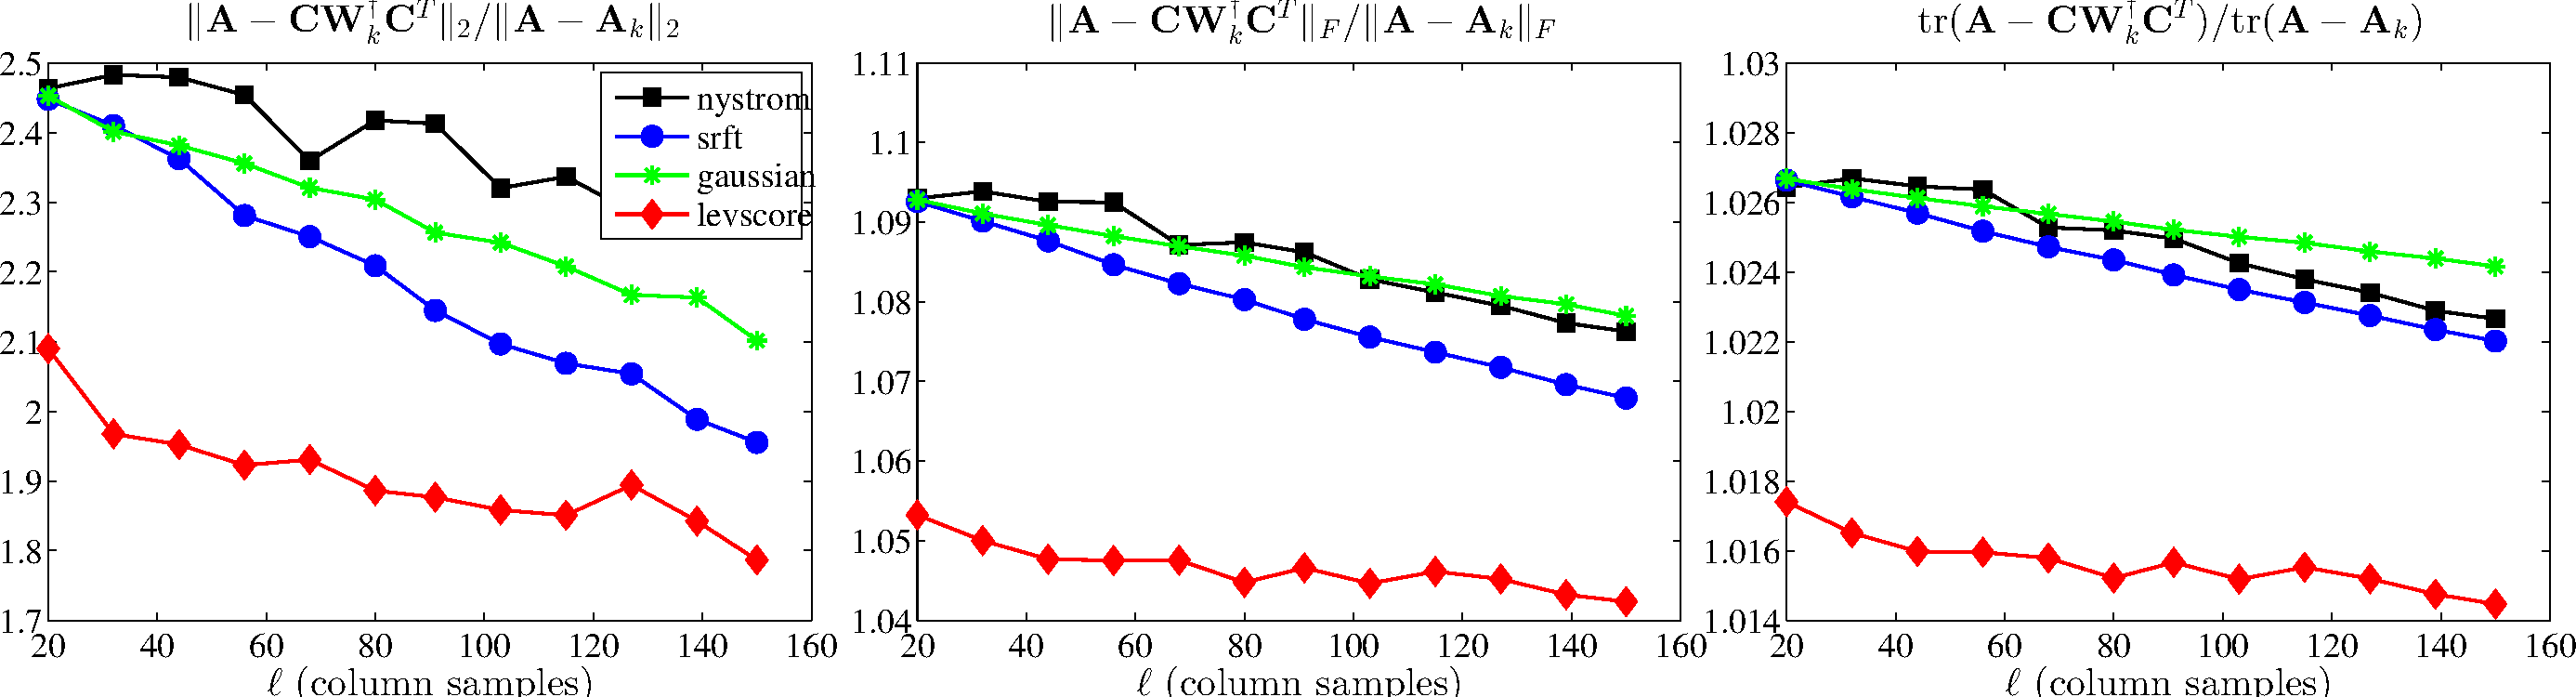
\includegraphics[width=6in, keepaspectratio=true]{figures/ch4/Abalonesigmapt15exact-methods-fixed-rank-errors}}
 
 \subfigure[AbaloneD, $\sigma = 1, k = 20$]{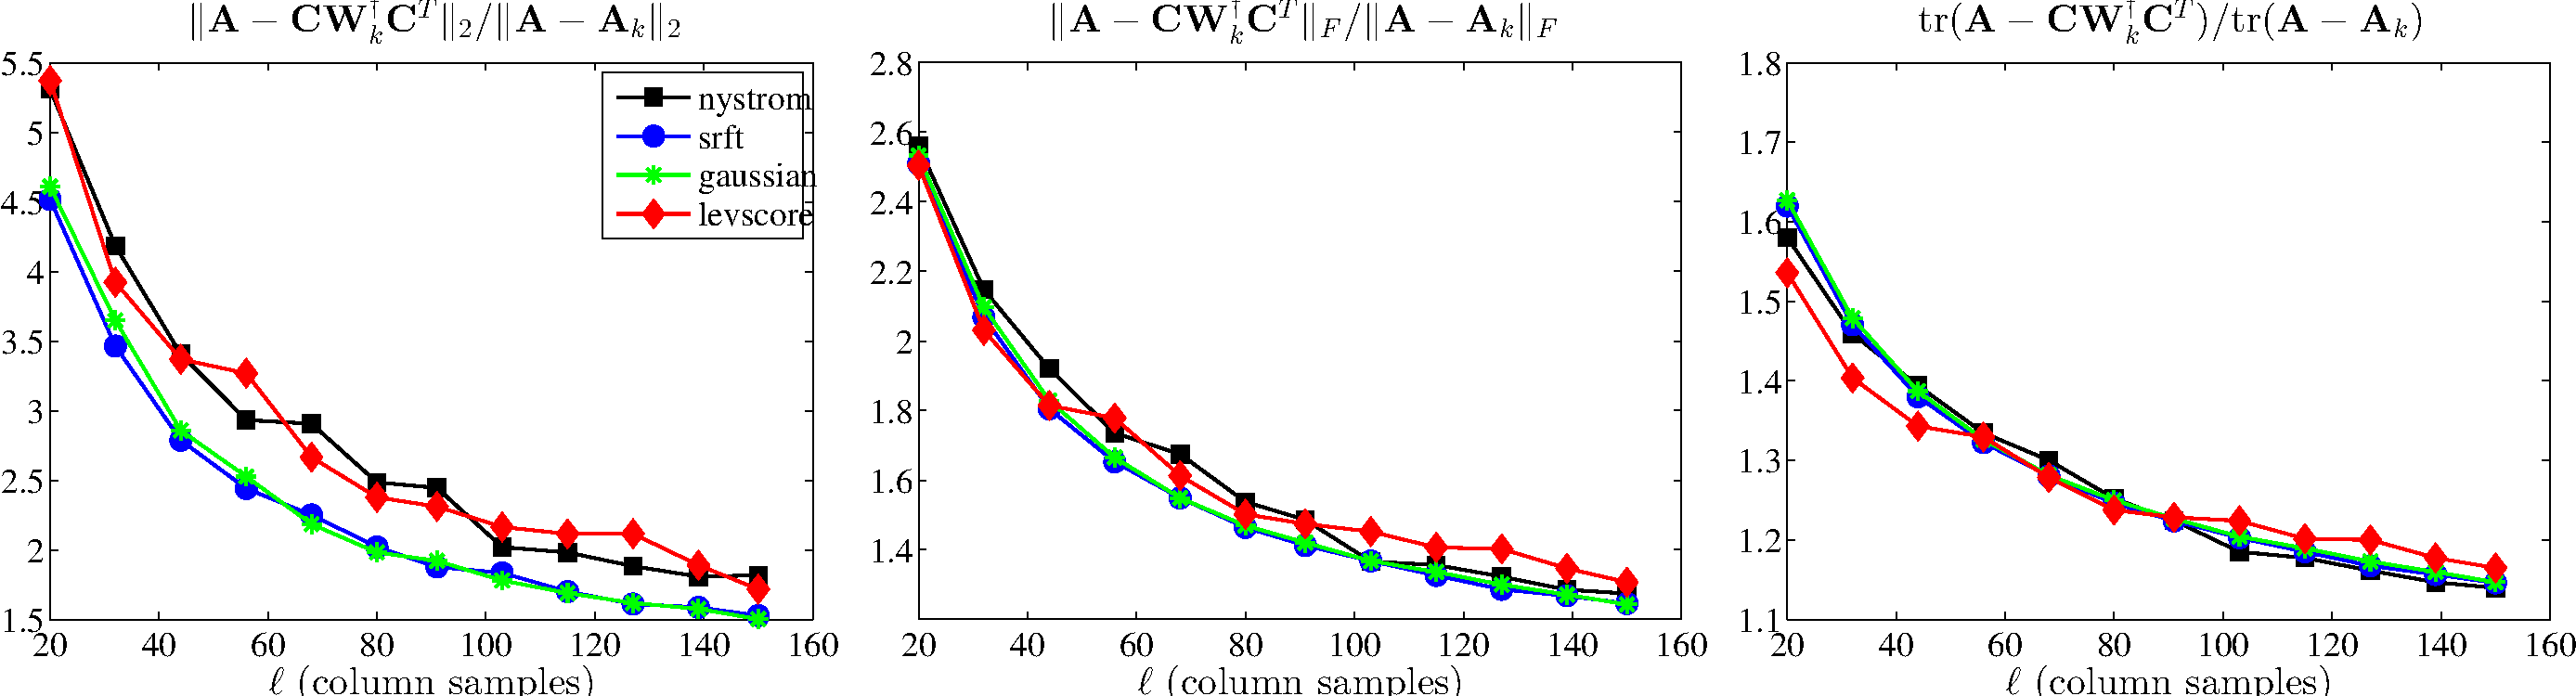
\includegraphics[width=6in, keepaspectratio=true]{figures/ch4/Abalonesigma1exact-methods-fixed-rank-errors}}
 
 \subfigure[WineD, $\sigma = 1, k = 20$]{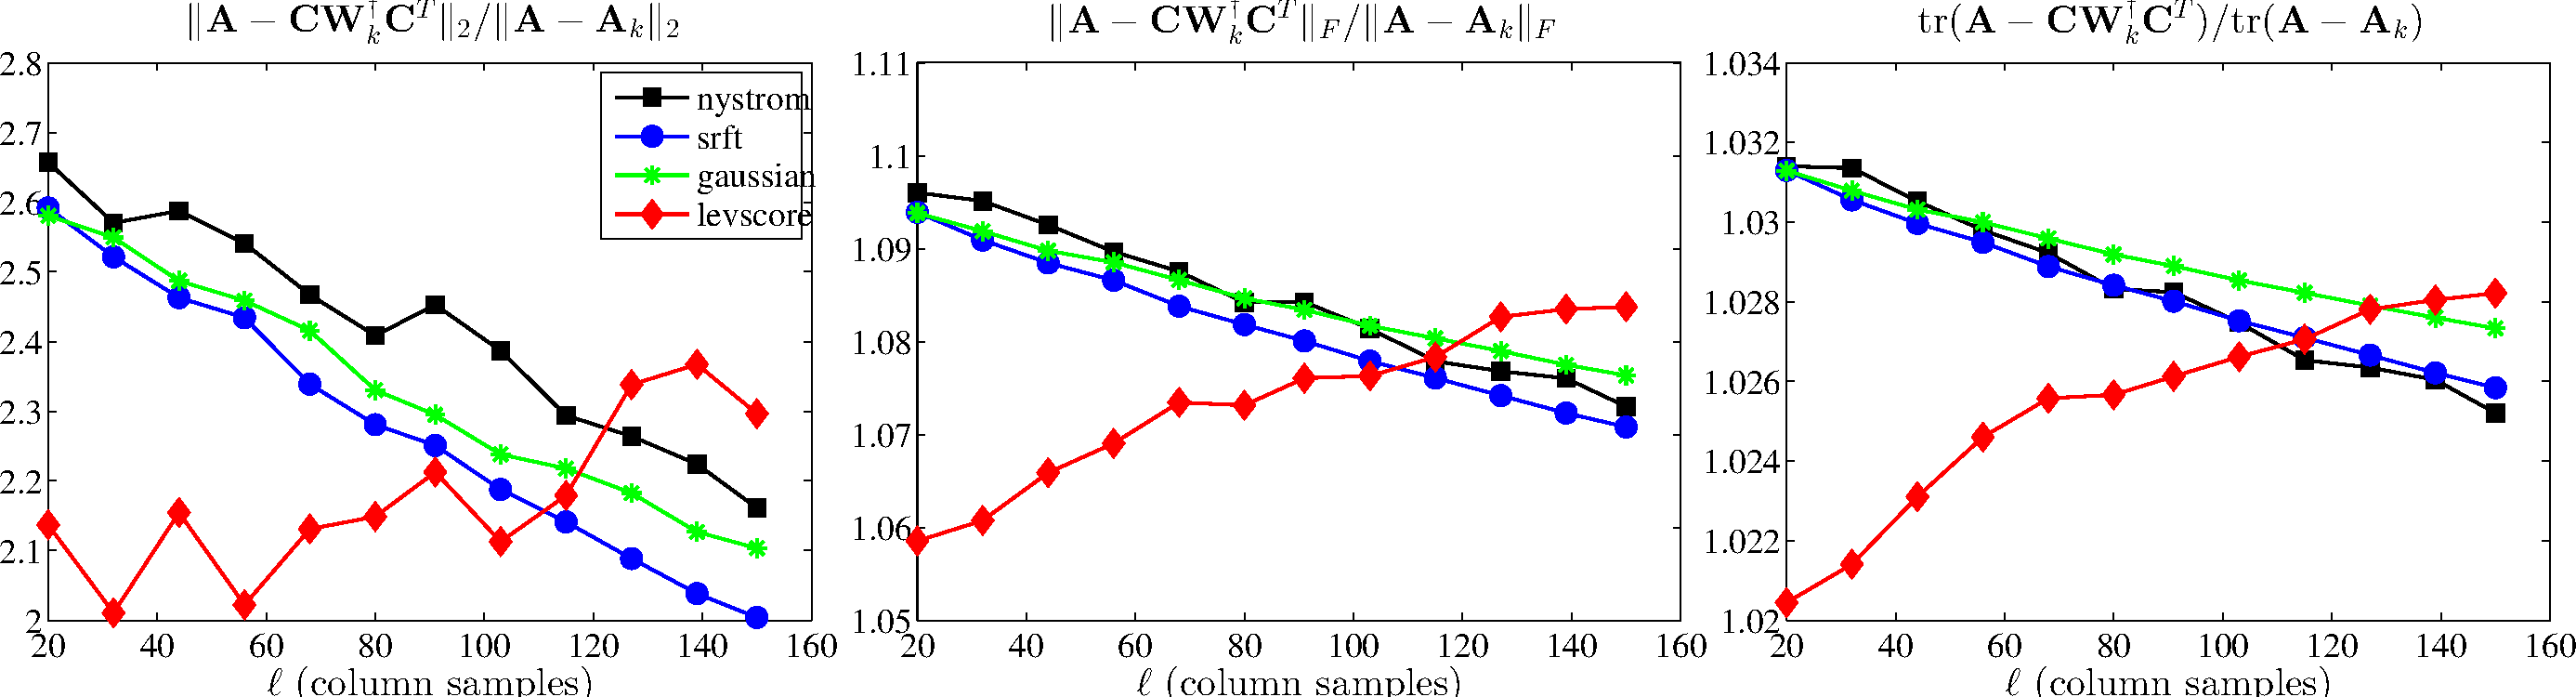
\includegraphics[width=6in, keepaspectratio=true]{figures/ch4/Winesigma1exact-methods-fixed-rank-errors}}
 
 \subfigure[WineD, $\sigma = 2.1, k = 20$]{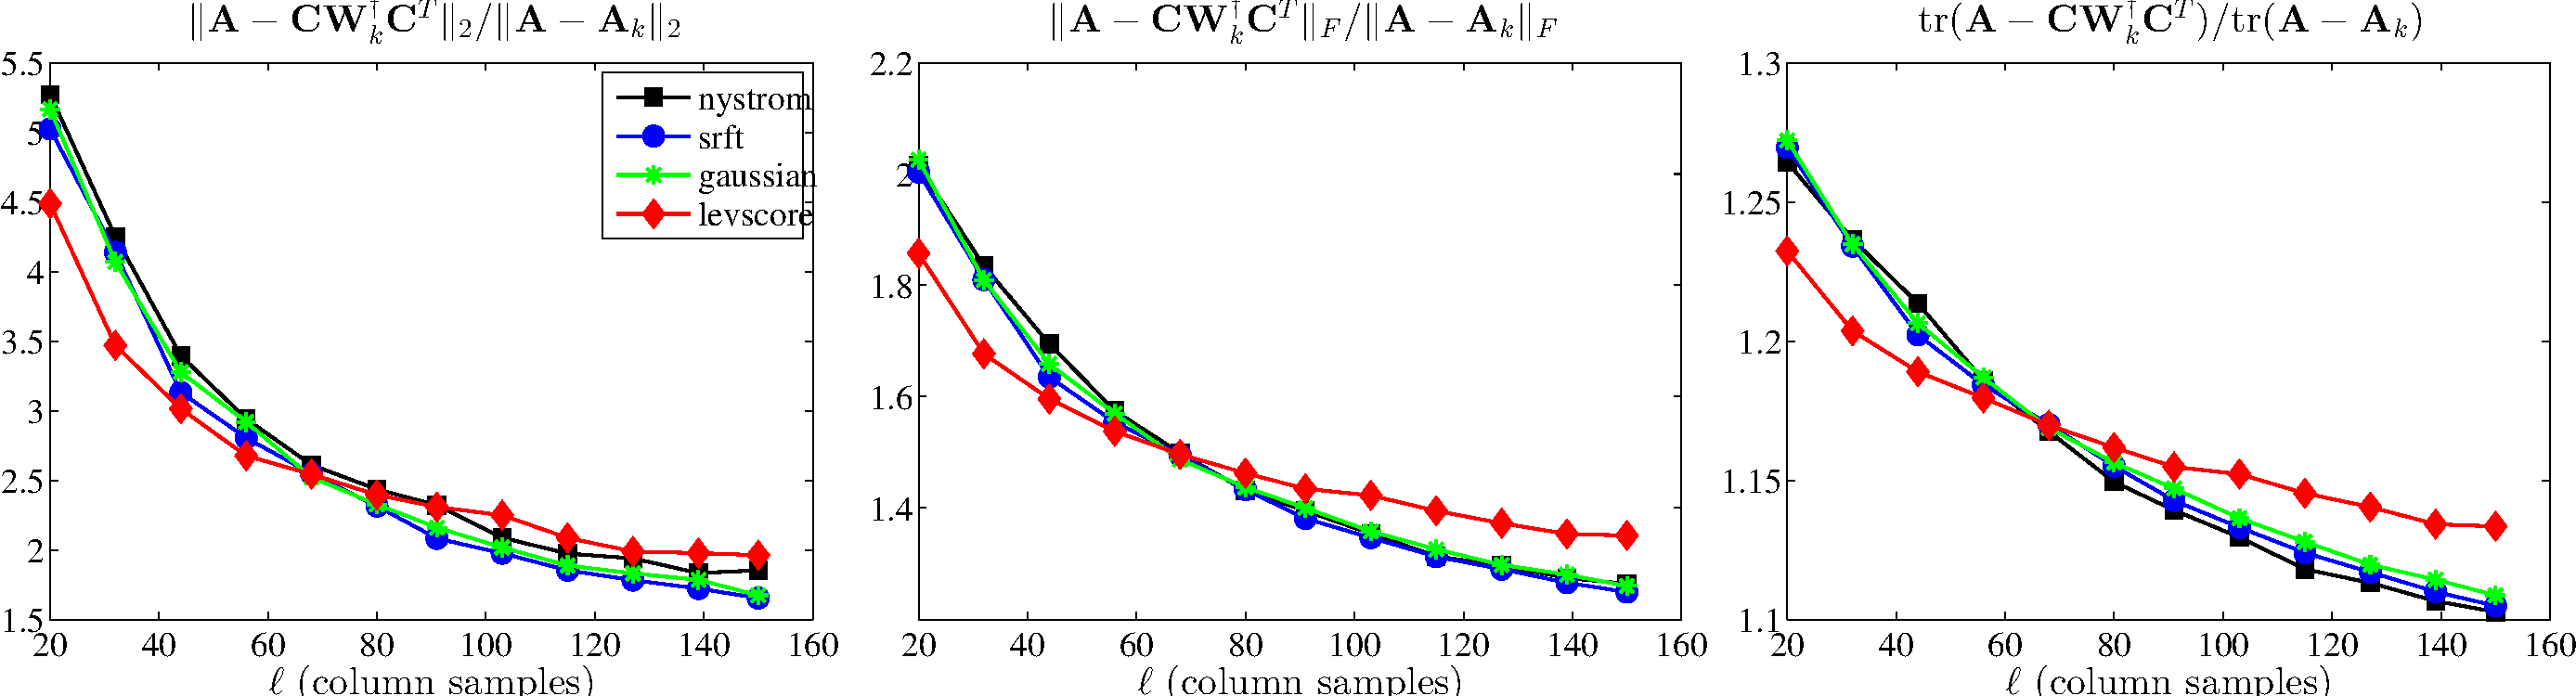
\includegraphics[width=6in, keepaspectratio=true]{figures/ch4/Winesigma2pt1exact-methods-fixed-rank-errors}}
 \caption[Relative errors of rank-restricted SPSD sketches of the dense RBFK matrices]{%
 {\sc Relative errors of rank-restricted SPSD sketches of the dense RBFK matrices.}
 The relative spectral, Frobenius, and trace-norm errors~\eqref{ch4:eqn:relerr2} of several rank-restricted
 SPSD sketches, as a function of the number of columns samples $\ell$, 
 for the dense RBFK matrices.}%
 \label{ch4:fig:denserbf-exact-errors-b}
\end{figure}

\begin{figure}[htp]
 \centering
 \subfigure[AbaloneS, $\sigma = .15, k = 20$]{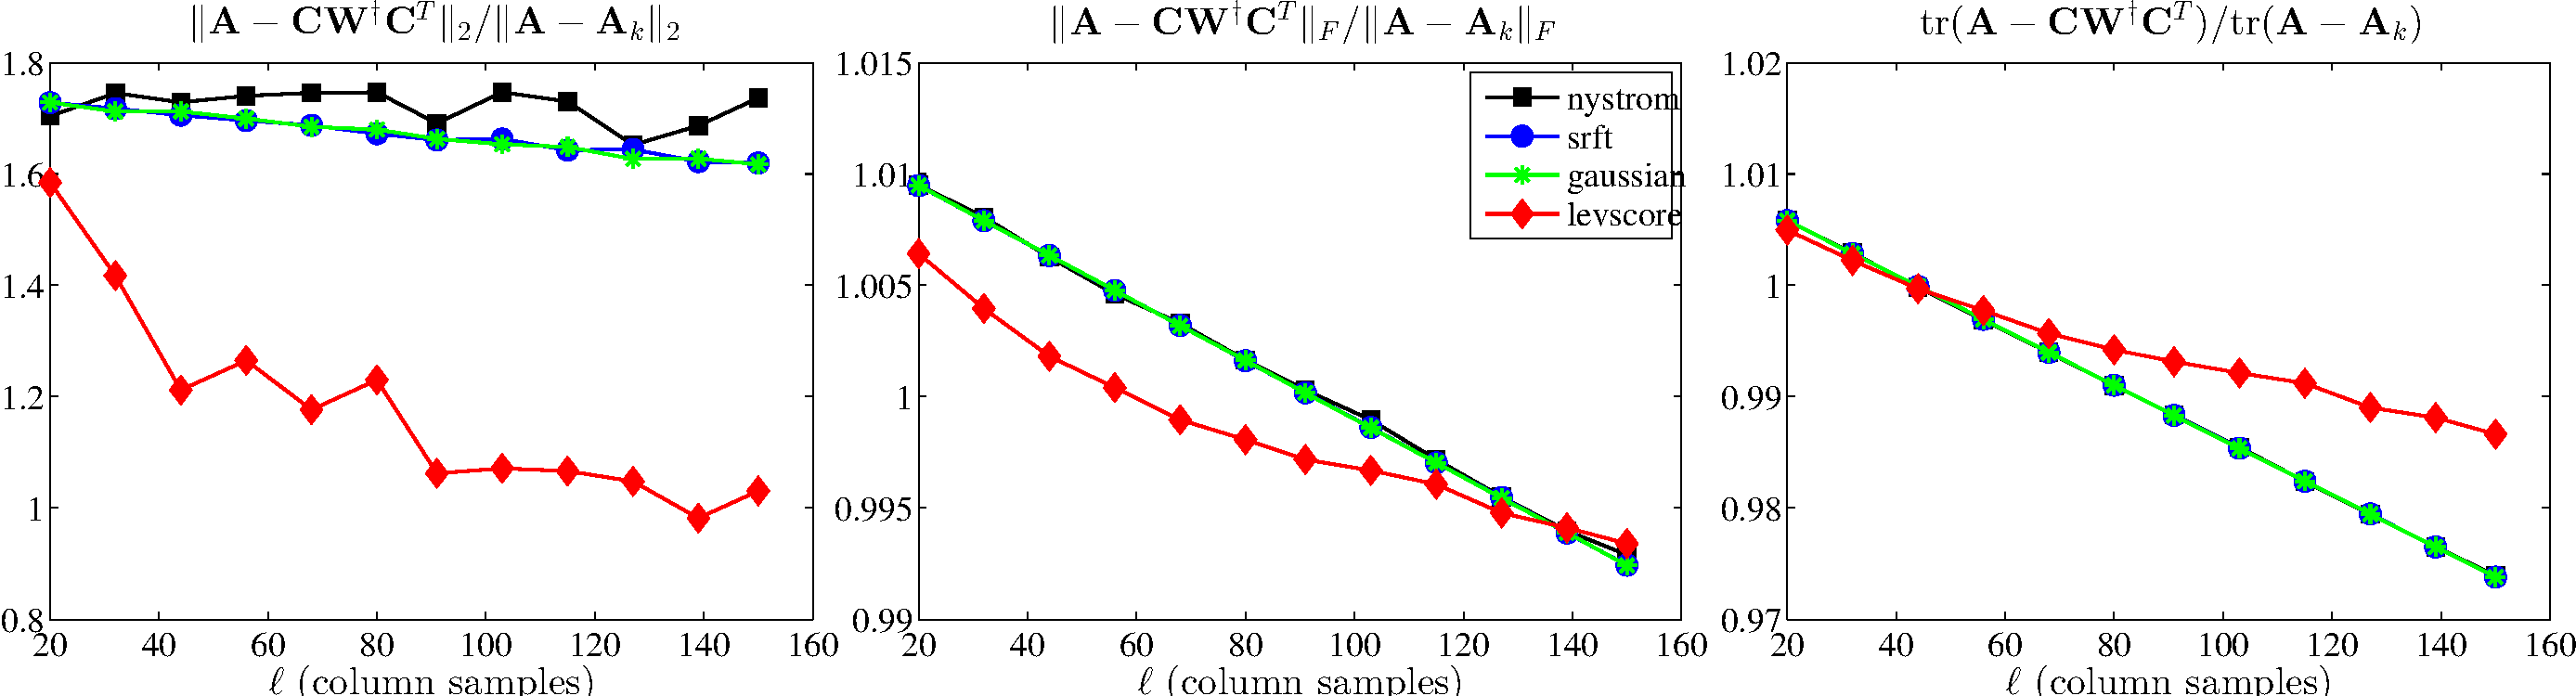
\includegraphics[width=6in, keepaspectratio=true]{figures/ch4/Abalonecompactsigmapt15exact-methods-nonfixed-rank-errors}}
 
 \subfigure[AbaloneS, $\sigma = 1, k = 20$]{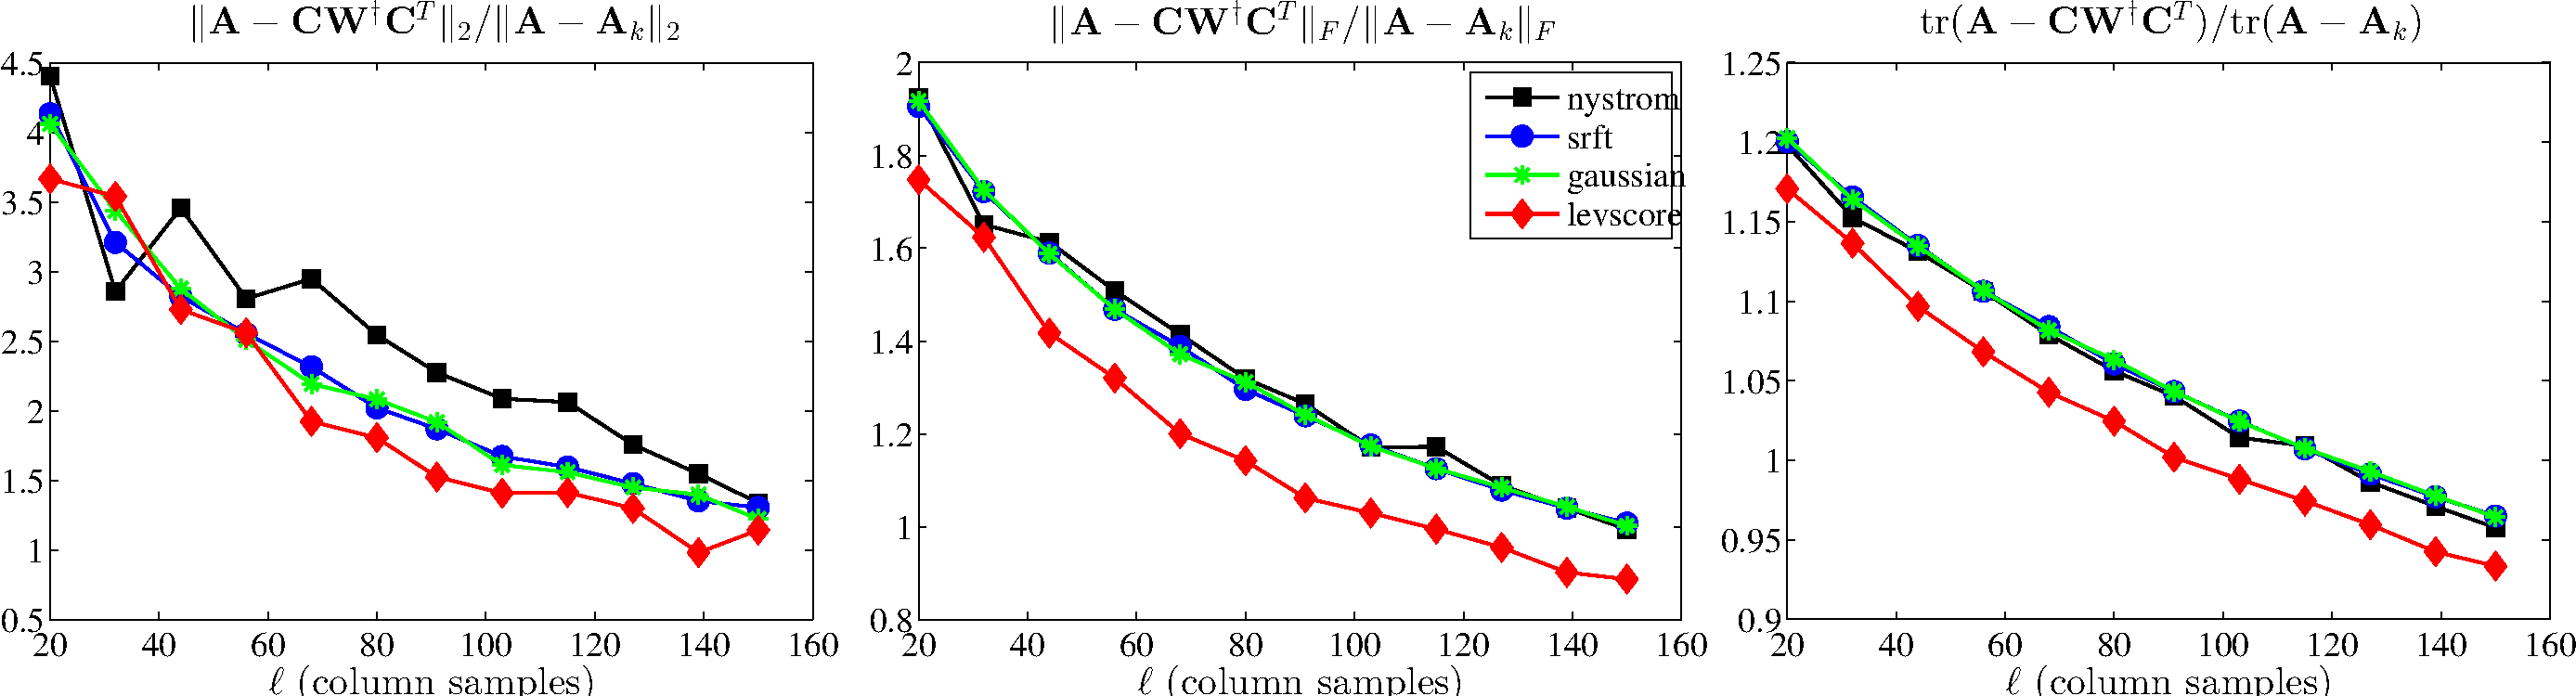
\includegraphics[width=6in, keepaspectratio=true]{figures/ch4/Abalonecompactsigma1exact-methods-nonfixed-rank-errors}}
 
 \subfigure[WineS, $\sigma = 1, k = 20$]{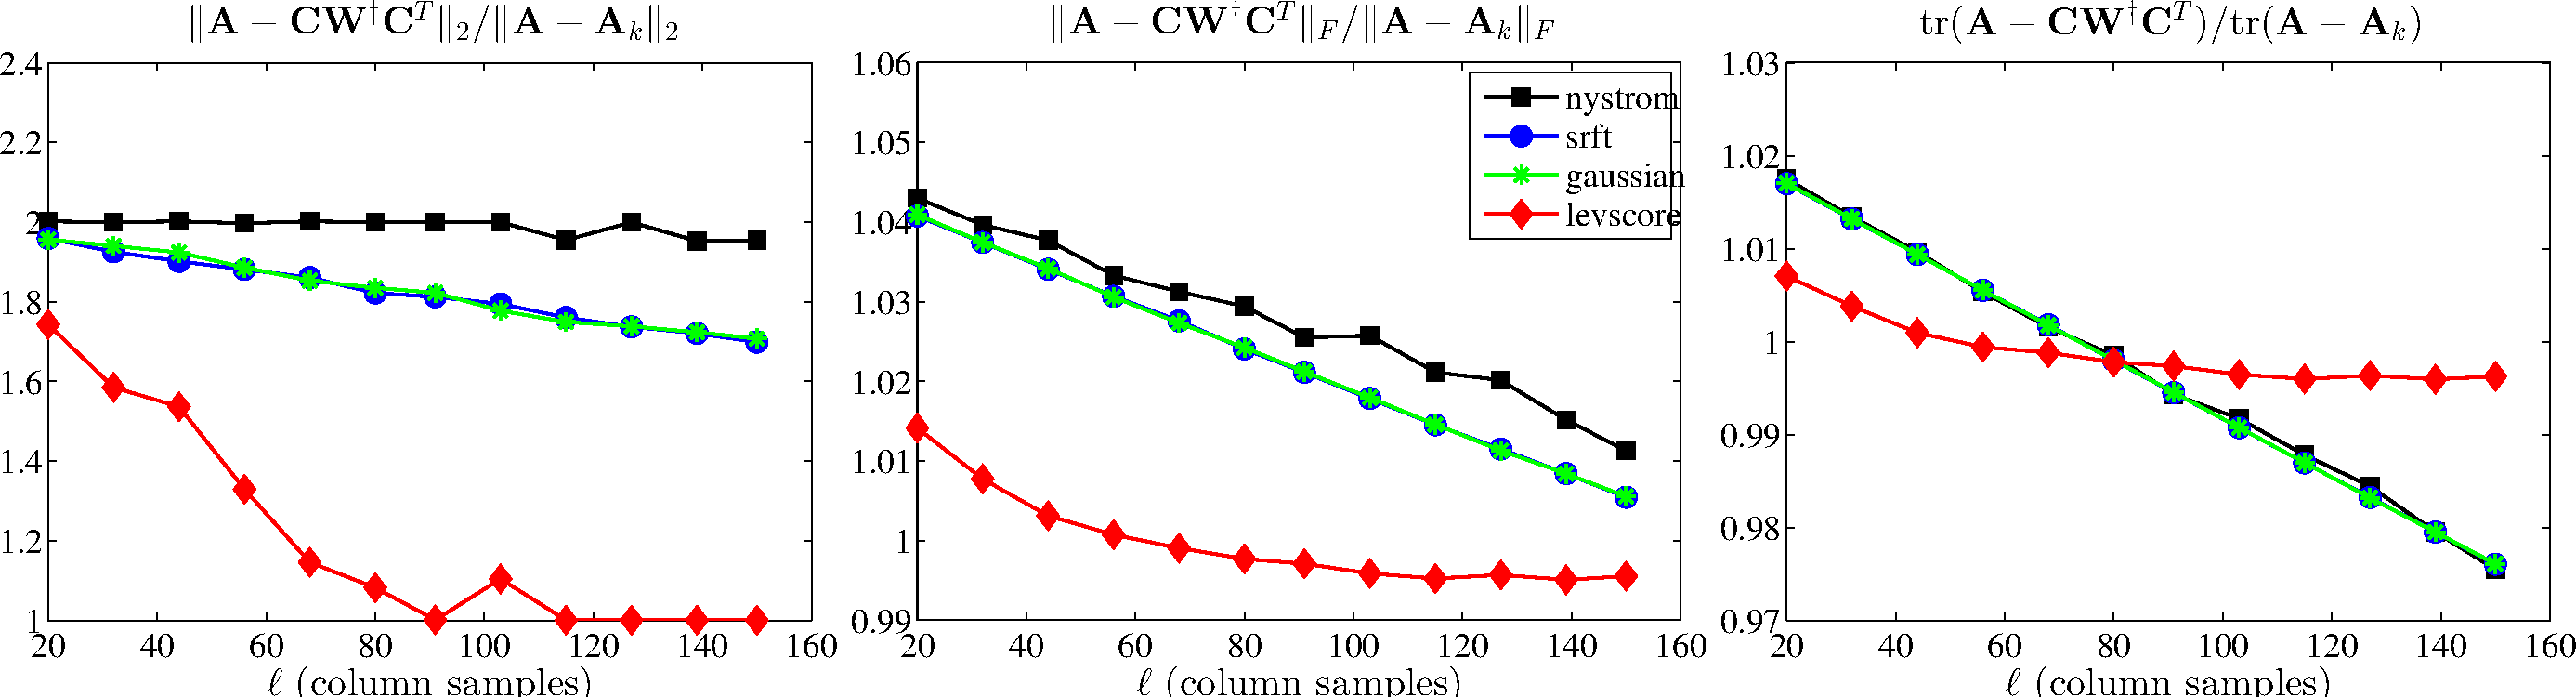
\includegraphics[width=6in, keepaspectratio=true]{figures/ch4/Winecompactsigma1exact-methods-nonfixed-rank-errors}}
 
 \subfigure[WineS, $\sigma = 2.1, k = 20$]{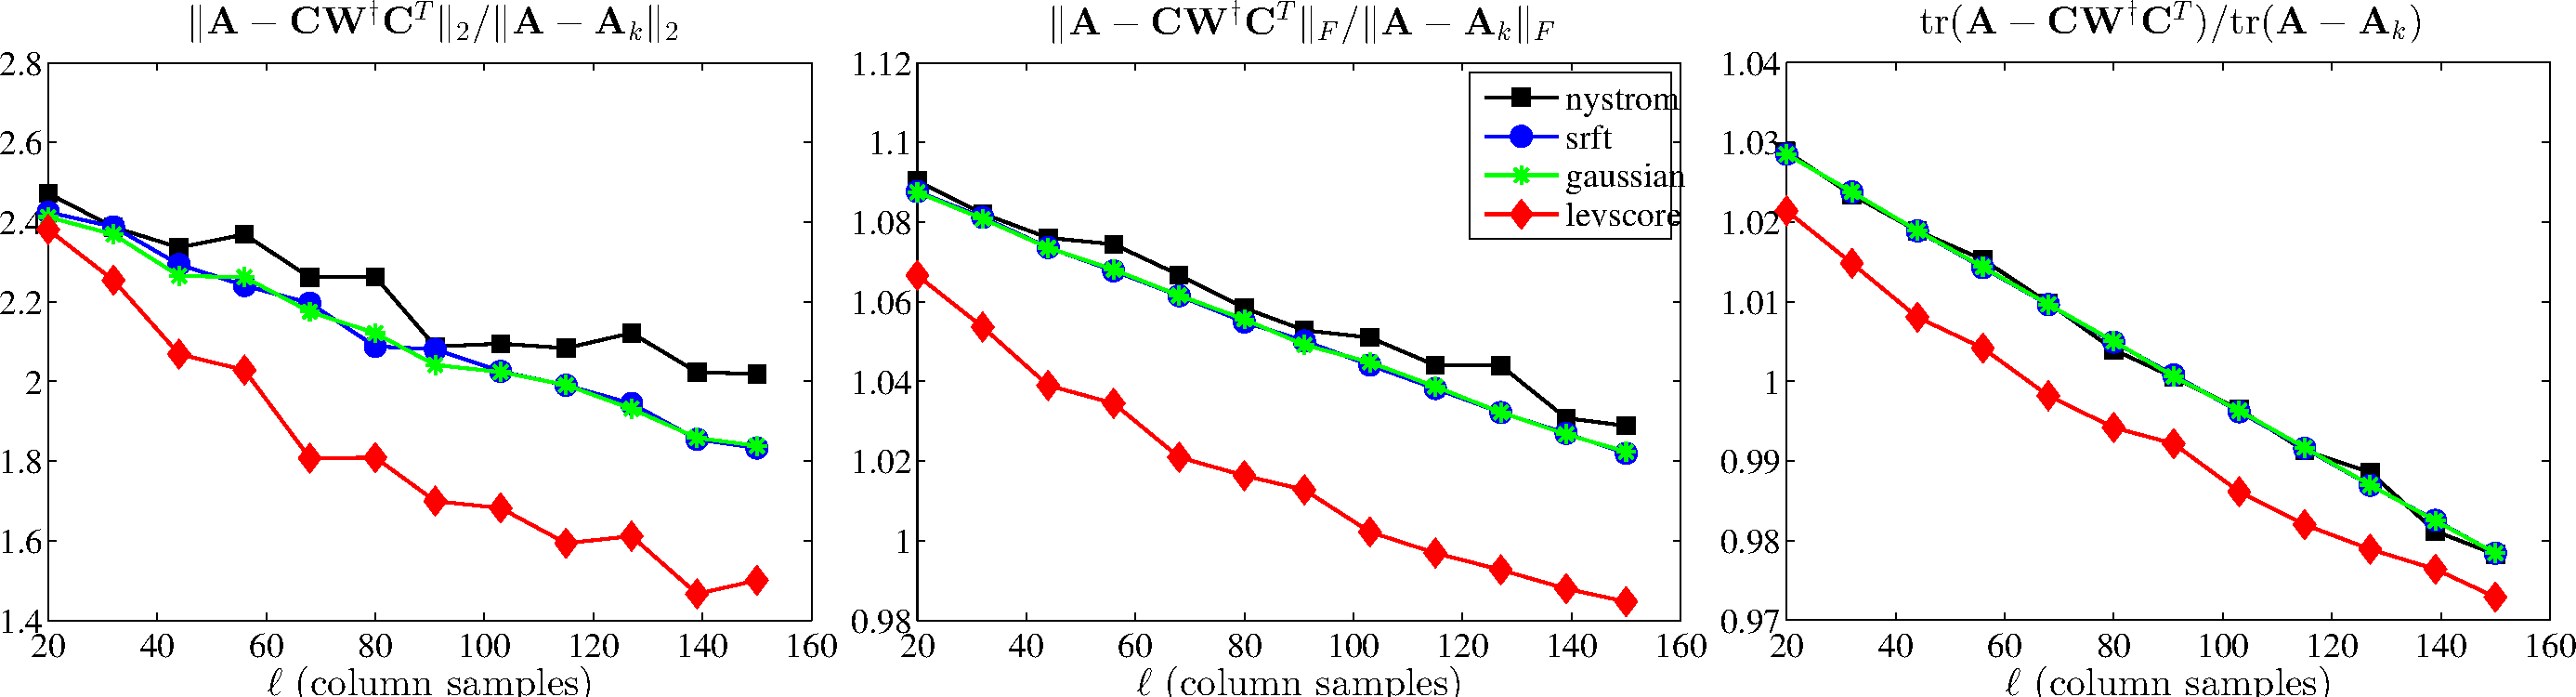
\includegraphics[width=6in, keepaspectratio=true]{figures/ch4/Winecompactsigma2pt1exact-methods-nonfixed-rank-errors}}
 \caption[Relative errors of non-rank-restricted SPSD sketches of the sparse RBFK matrices]{%
 {\sc Relative errors of non-rank-restricted SPSD sketches of the sparse RBFK matrices.}
 The relative spectral, Frobenius, and trace-norm errors~\eqref{ch4:eqn:relerr1} of several non-rank-restricted
 SPSD sketches, as a function of the number of columns samples $\ell$, 
 for the sparse RBFK matrices.}%
 \label{ch4:fig:sparserbf-exact-errors-a}
\end{figure}

\begin{figure}[htp]
 \centering
 \subfigure[AbaloneS, $\sigma = .15, k = 20$]{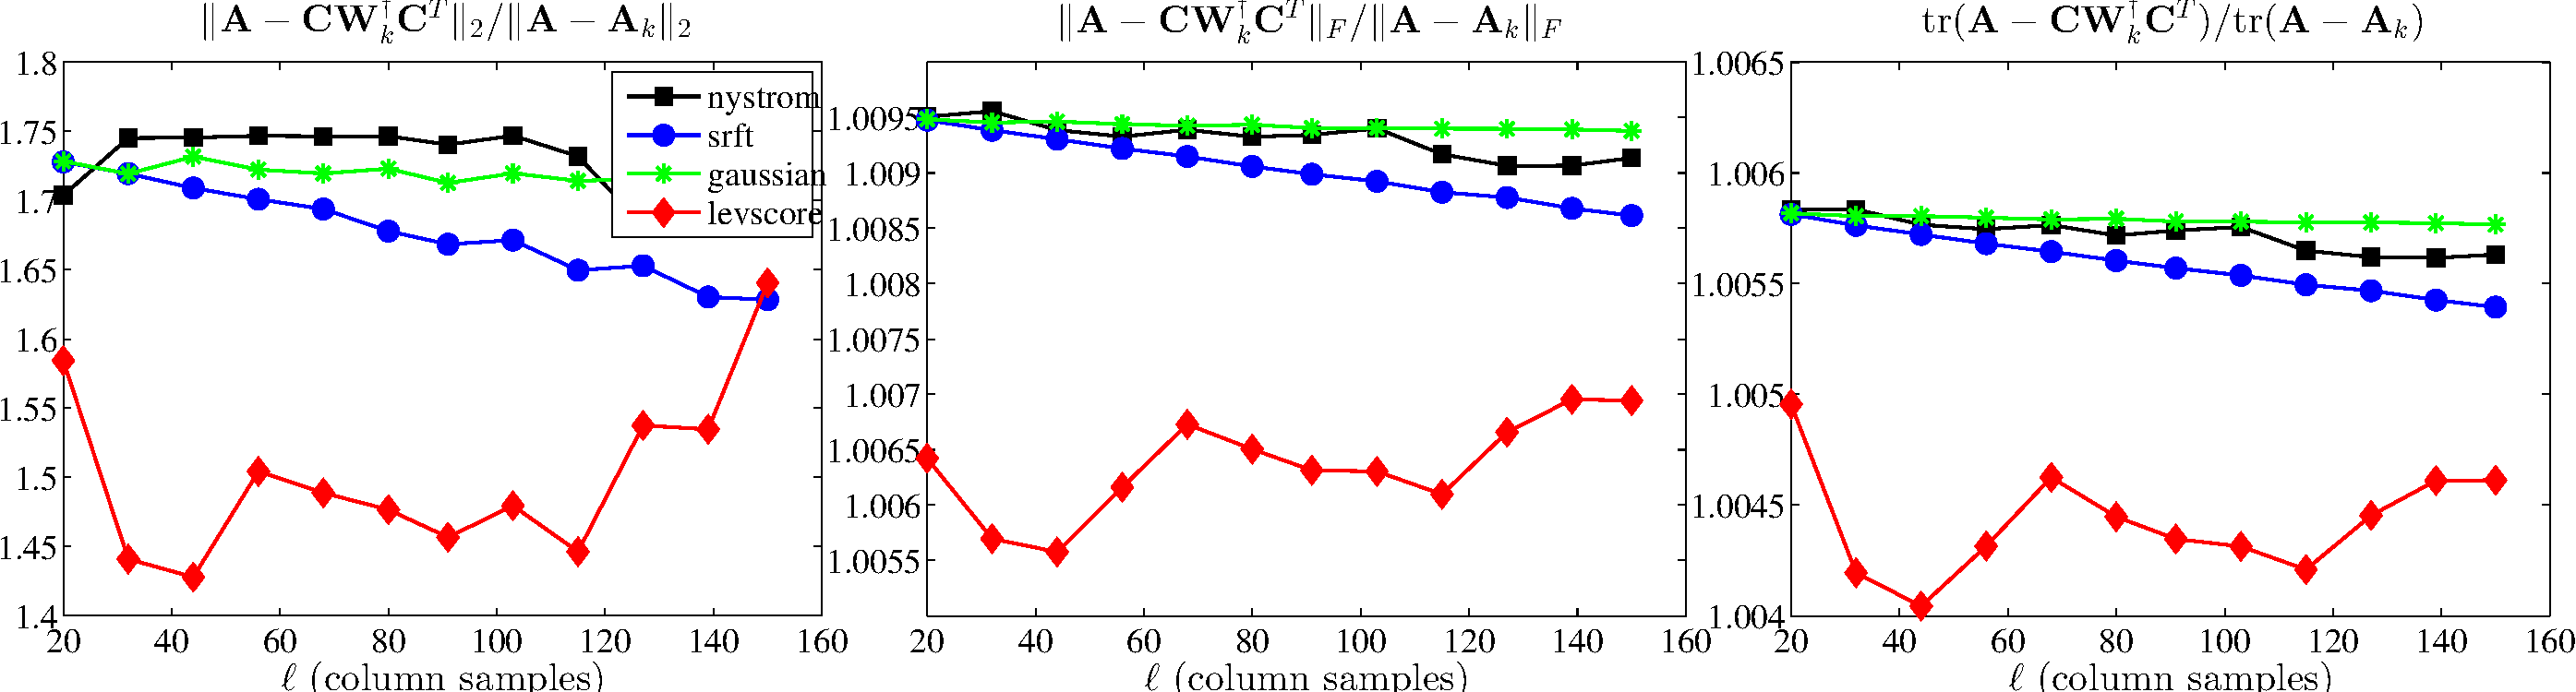
\includegraphics[width=6in, keepaspectratio=true]{figures/ch4/Abalonecompactsigmapt15exact-methods-fixed-rank-errors}}
 
 \subfigure[AbaloneS, $\sigma = 1, k = 20$]{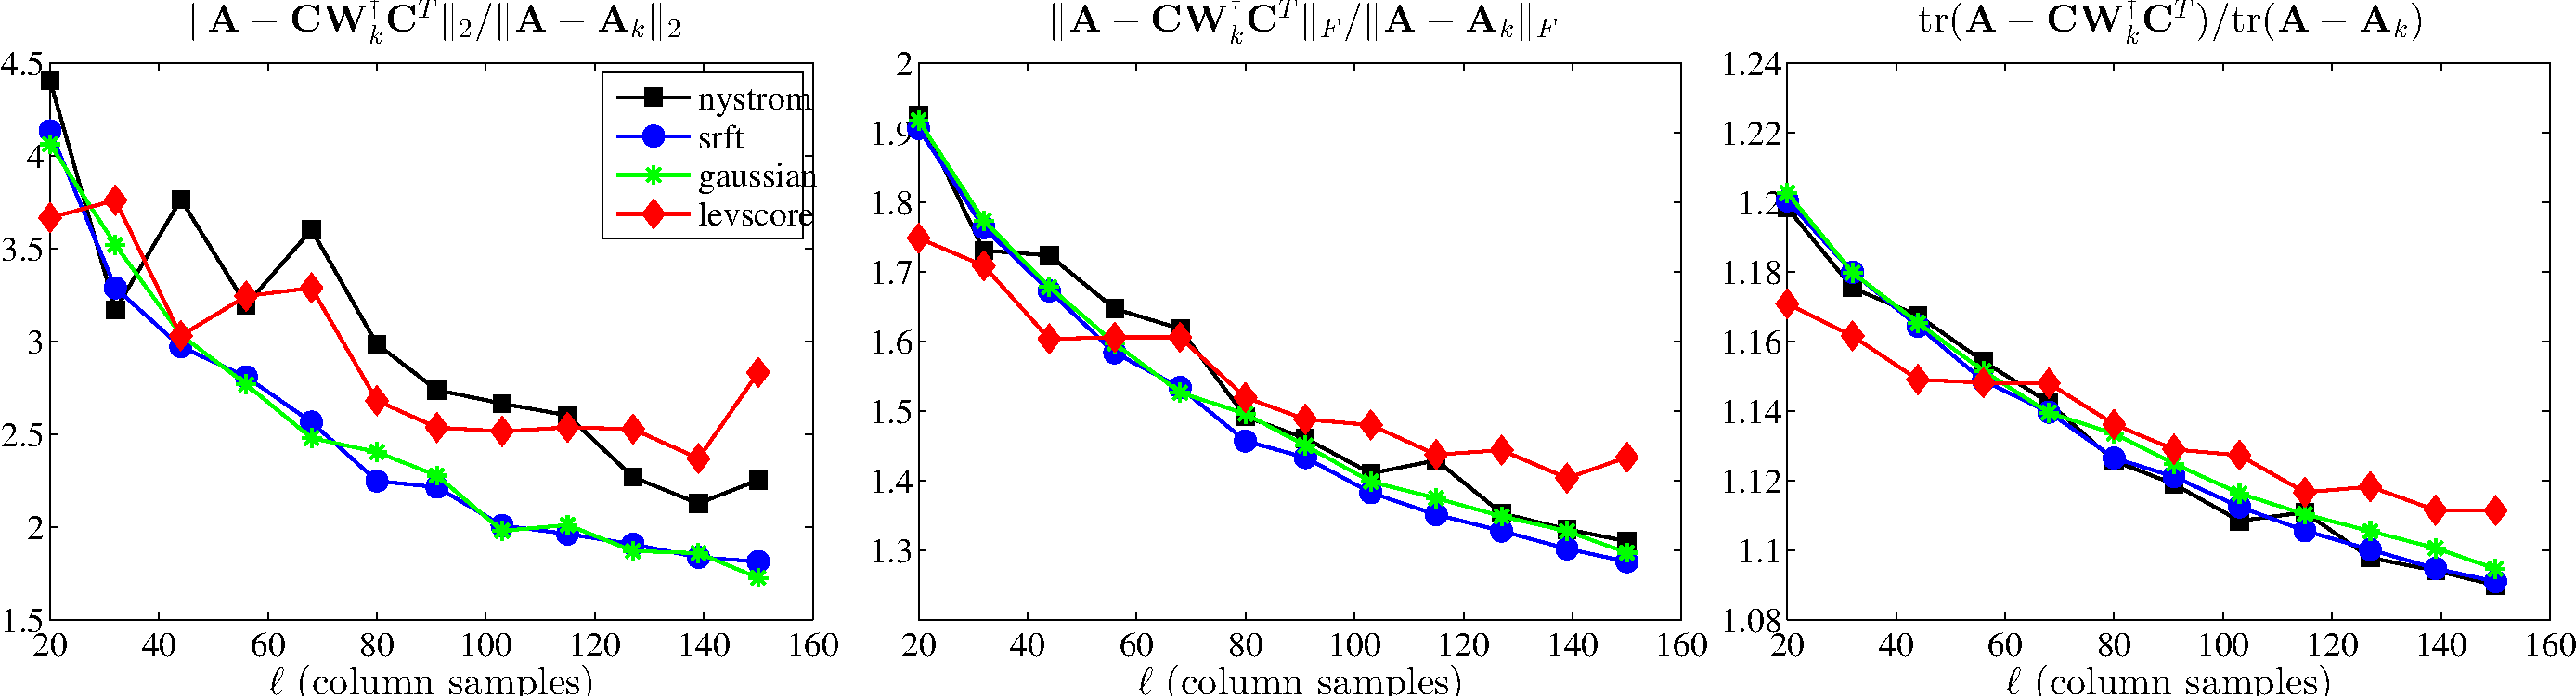
\includegraphics[width=6in, keepaspectratio=true]{figures/ch4/Abalonecompactsigma1exact-methods-fixed-rank-errors}}
 
 \subfigure[WineS, $\sigma = 1, k = 20$]{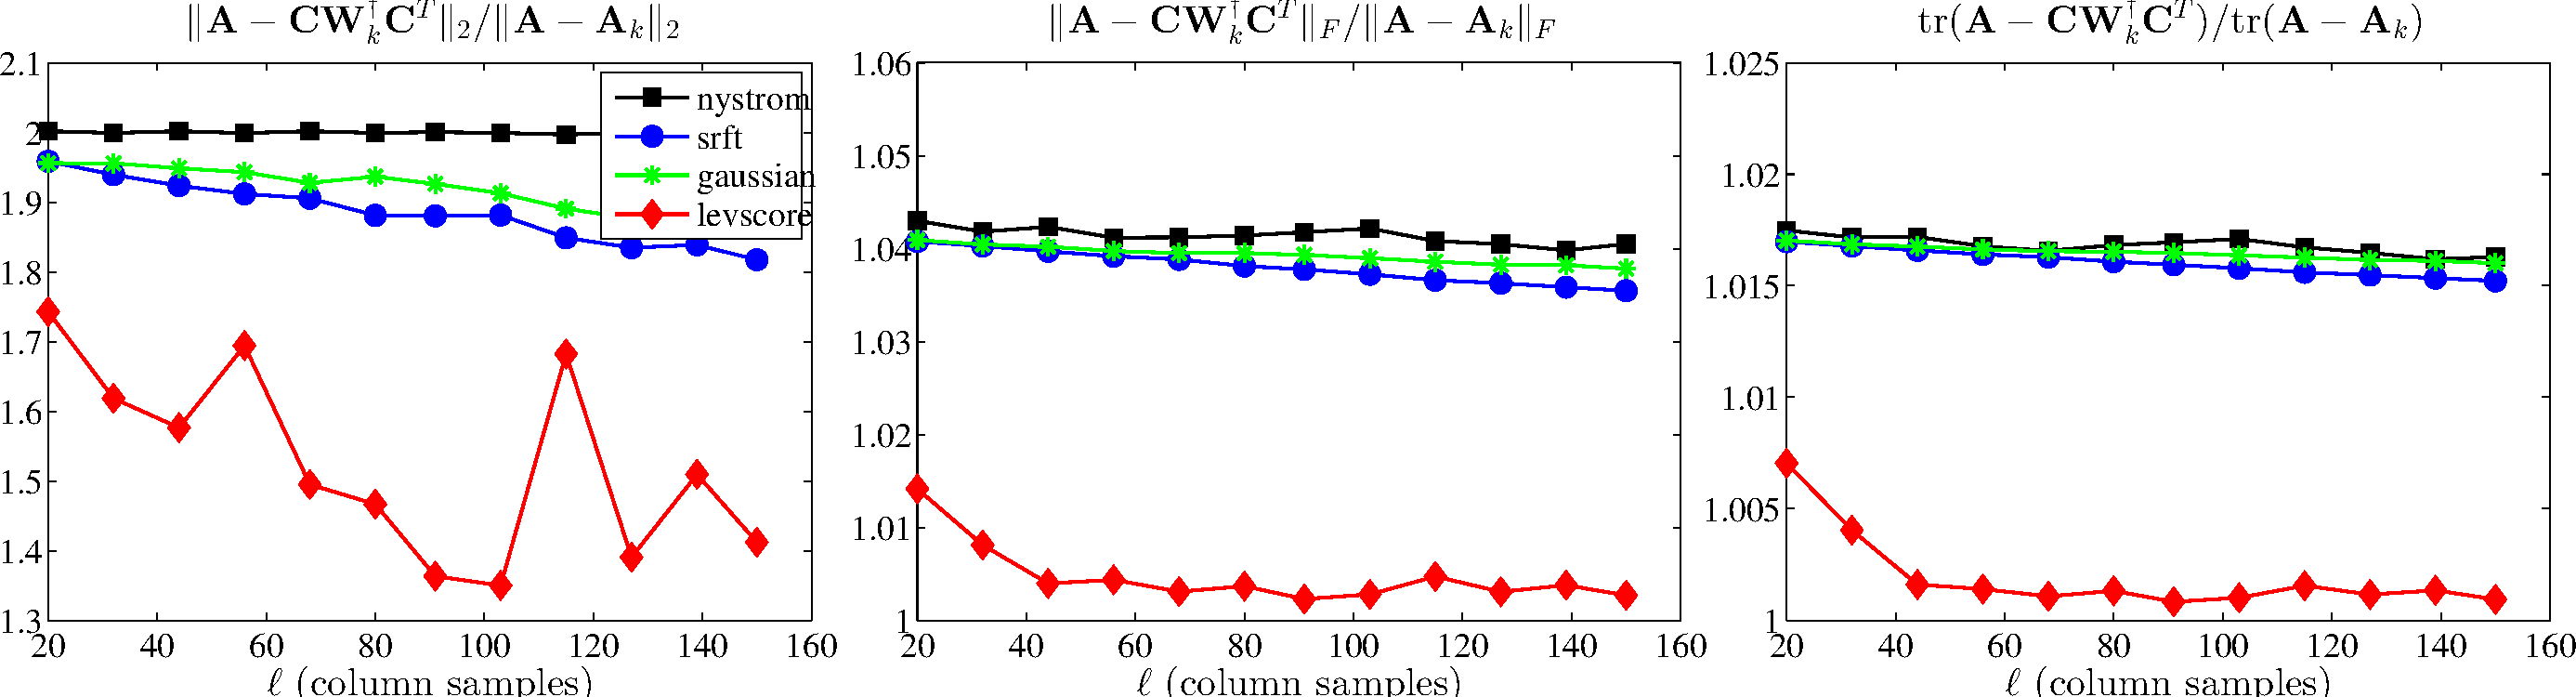
\includegraphics[width=6in, keepaspectratio=true]{figures/ch4/Winecompactsigma1exact-methods-fixed-rank-errors}}
 
 \subfigure[WineS, $\sigma = 2.1, k = 20$]{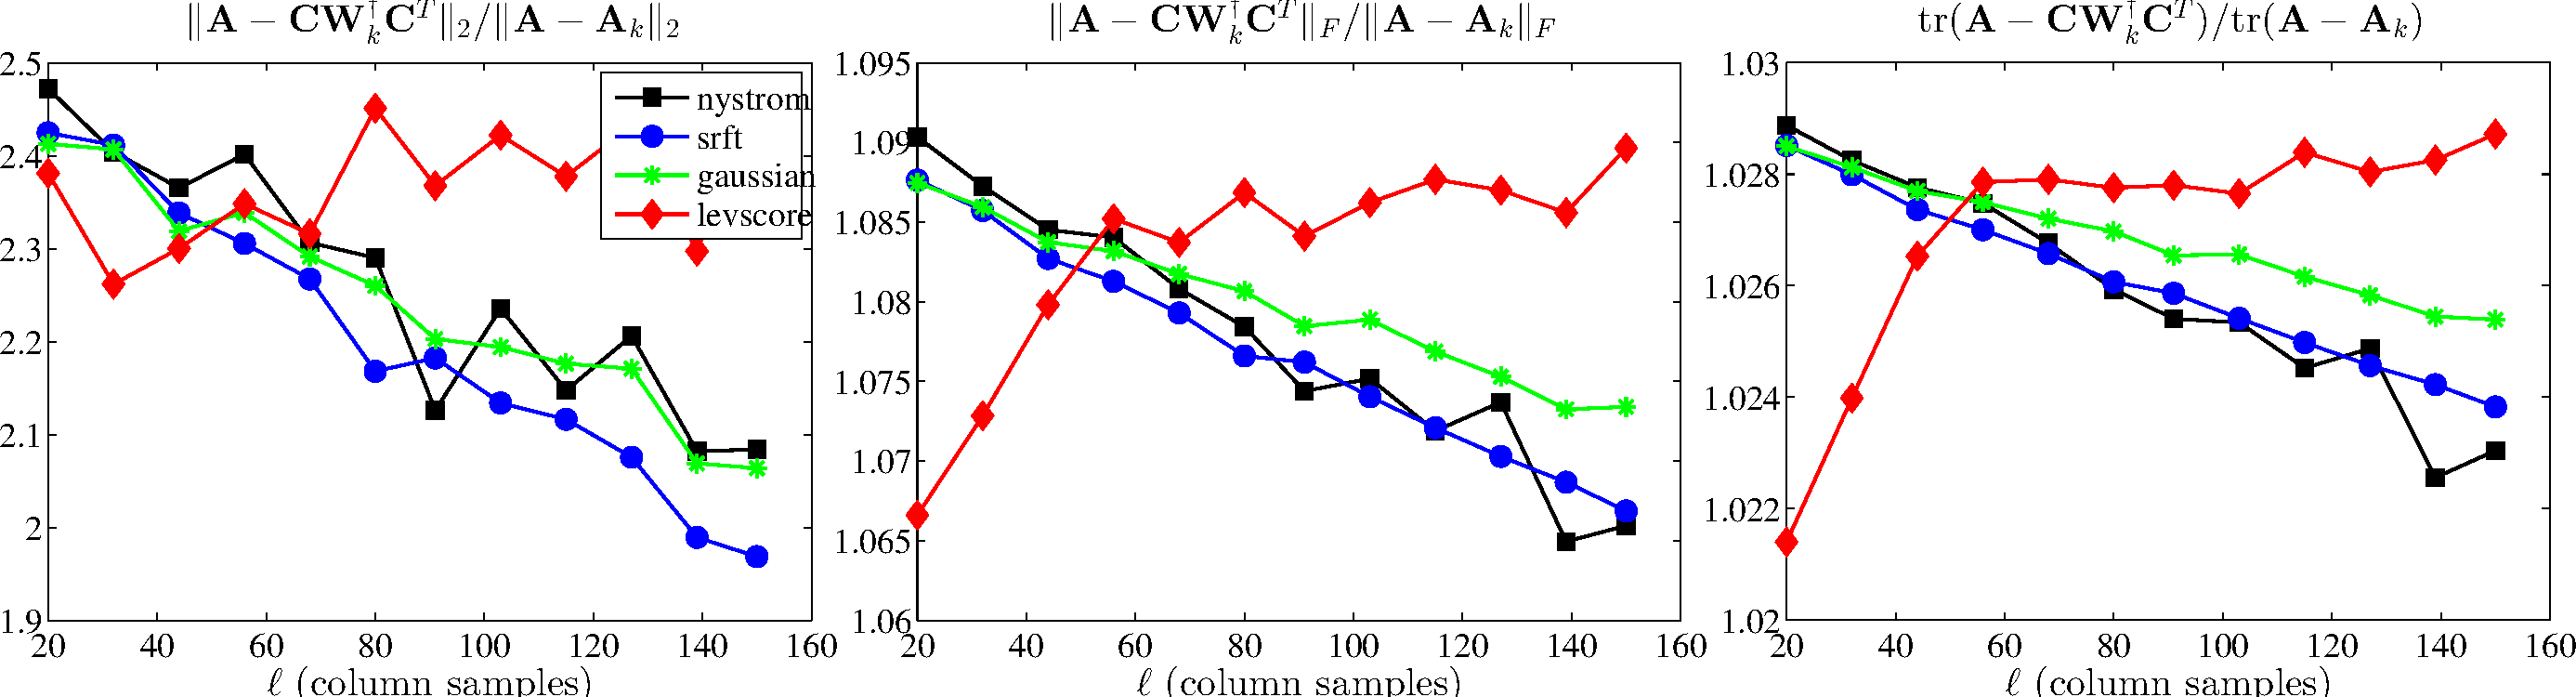
\includegraphics[width=6in, keepaspectratio=true]{figures/ch4/Winecompactsigma2pt1exact-methods-fixed-rank-errors}}
 \caption[Relative errors of rank-restricted SPSD sketches of the sparse RBFK matrices]{%
 {\sc Relative errors of rank-restricted SPSD sketches of the sparse RBFK matrices.}
 The relative spectral, Frobenius, and trace-norm errors~\eqref{ch4:eqn:relerr2} of several rank-restricted
 SPSD sketches, as a function of the number of columns samples $\ell$, 
 for the sparse RBFK matrices. }%
 \label{ch4:fig:sparserbf-exact-errors-b}
\end{figure}

Figures~\ref{ch4:fig:denserbf-exact-errors-a}--\ref{ch4:fig:sparserbf-exact-errors-b} 
present 
the reconstruction error results for sampling and mixture methods 
applied to several dense RBF and sparse RBF kernels.
Several observations are worth making about the results presented in these 
figures.
\begin{itemize}
\item
For the non-rank-restricted results, all of the methods have errors that 
decrease with increasing $\ell$.
In particular, for larger values of $\sigma$ and for denser matrices, the 
decrease is somewhat more regular, and the four methods tend to perform 
similarly.
For larger values of $\sigma$ and sparser matrices, leverage
score sampling is somewhat better.
This parallels what we observed with the linear kernels, except that here the 
leverage score sampling is somewhat better for all values of $\ell$.
\item
For the non-rank-restricted results for the smaller values of $\sigma$, 
leverage score sampling tends to be much better than uniform sampling and 
mixture-based methods.
For the sparse matrices, however, this effect saturates. We again observe 
(especially when $\sigma$ is smaller in AbaloneS and WineS) the tradeoff we 
observed previously with the Laplacian matrices: leverage score sampling is 
better when $\ell$ is moderately larger than $k$, while uniform sampling and 
random mixtures are better when $\ell$ is much larger than $k$.
\item
For the rank-restricted results, we see that when $\sigma$ is large, all 
of the results tend to perform similarly.
(The exception to this is WineS, for which leverage score sampling starts out 
much better than other methods and then gets worse as $\ell$ is increased.)
On the other hand, when $\sigma$ is small, the results are more complex.
Leverage score sampling is typically much better than other methods, 
although the results are quite choppy as a function of $\ell$, and in some 
cases the effect diminishes as $\ell$ is increased.
\end{itemize}
Recall from Table~\ref{ch4:table:datasets_stats} that for smaller values of 
$\sigma$ and for sparser kernels, the SPSD matrices are less 
well-approximated by low-rank matrices, and they have more heterogeneous 
leverage scores.
Thus, they are more similar to the Laplacian matrices than the linear kernel 
matrices; and this suggests (as we have observed) that leverage score sampling 
should perform better than uniform column sampling and 
mixture-based schemes in these two cases.
In particular, nowhere do we see that leverage score sampling performs much 
worse than other methods, as we saw with the rank-restricted linear 
kernel results.

\subsubsection{Summary of comparison of sampling and mixture-based SPSD Sketches}

Several summary observations can be made about sampling versus mixture-based SPSD sketches
for the matrices we have considered.
\begin{itemize}
\item
Linear kernels and to a lesser extent dense RBF kernels with larger $\sigma$
parameter have relatively low rank and relatively uniform leverage scores, 
and in these cases uniform sampling does quite well.
These matrices correspond most closely with those that have been studied 
previously in the machine learning literature, and for these matrices our 
results are in agreement with that prior work.
\item
Sparsifying RBF kernels and/or choosing a smaller $\sigma$ parameter tends
to make these kernels worse approximated by low-rank matrices and to 
have more heterogeneous leverage scores.
In general, these two properties need not be directly related: the spectrum is 
a property of eigenvalues, while the leverage scores are determined by the 
eigenvectors. However, in the matrices we examined they are related, in that 
matrices with more slowly decaying spectra also often have more 
heterogeneous leverage scores.
\item
For dense RBF kernels with smaller $\sigma$ and sparse RBF kernels, leverage 
score sampling tends to do much better than other methods.
Interestingly, the sparse RBF kernels have many properties of very sparse 
Laplacian kernels corresponding to relatively unstructured informatics 
graphs.

\item
Reconstruction quality under leverage score sampling saturates, as a 
function of choosing more samples $\ell$; this is seen both for 
non-rank-restricted and rank-restricted situations.
As a consequence, there is often a transition between leverage score sampling
or other methods being better as $\ell$ increases.
\item
Although they are potentially ill-conditioned, non-rank-restricted approximations 
behave better in terms of reconstruction quality.
Rank-constrained approximations tend to have much more complicated behavior
as a function of increasing the number of samples $\ell$, including choppier
and non-monotonic behavior.
This is particularly severe for leverage score sampling, but it occurs with
other methods. Other forms of regularization might be appropriate.
\end{itemize}
In general, \emph{all} of the sampling and mixture-based sketches we considered 
perform \emph{much} better on the SPSD matrices we considered than both the previous
worst-case bounds (e.g.,~\cite{DM05,KMT12}) 
and the bounds derived in this chapter would suggest.
Even the worst results correspond to single-digit approximation 
factors in relative scale.

\section{A comparison with projection-based low-rank approximations}
\label{ch4:sec:comparison}

\begin{figure}[tb!]
 \centering
 \subfigure[Gnutella, $k=20$]{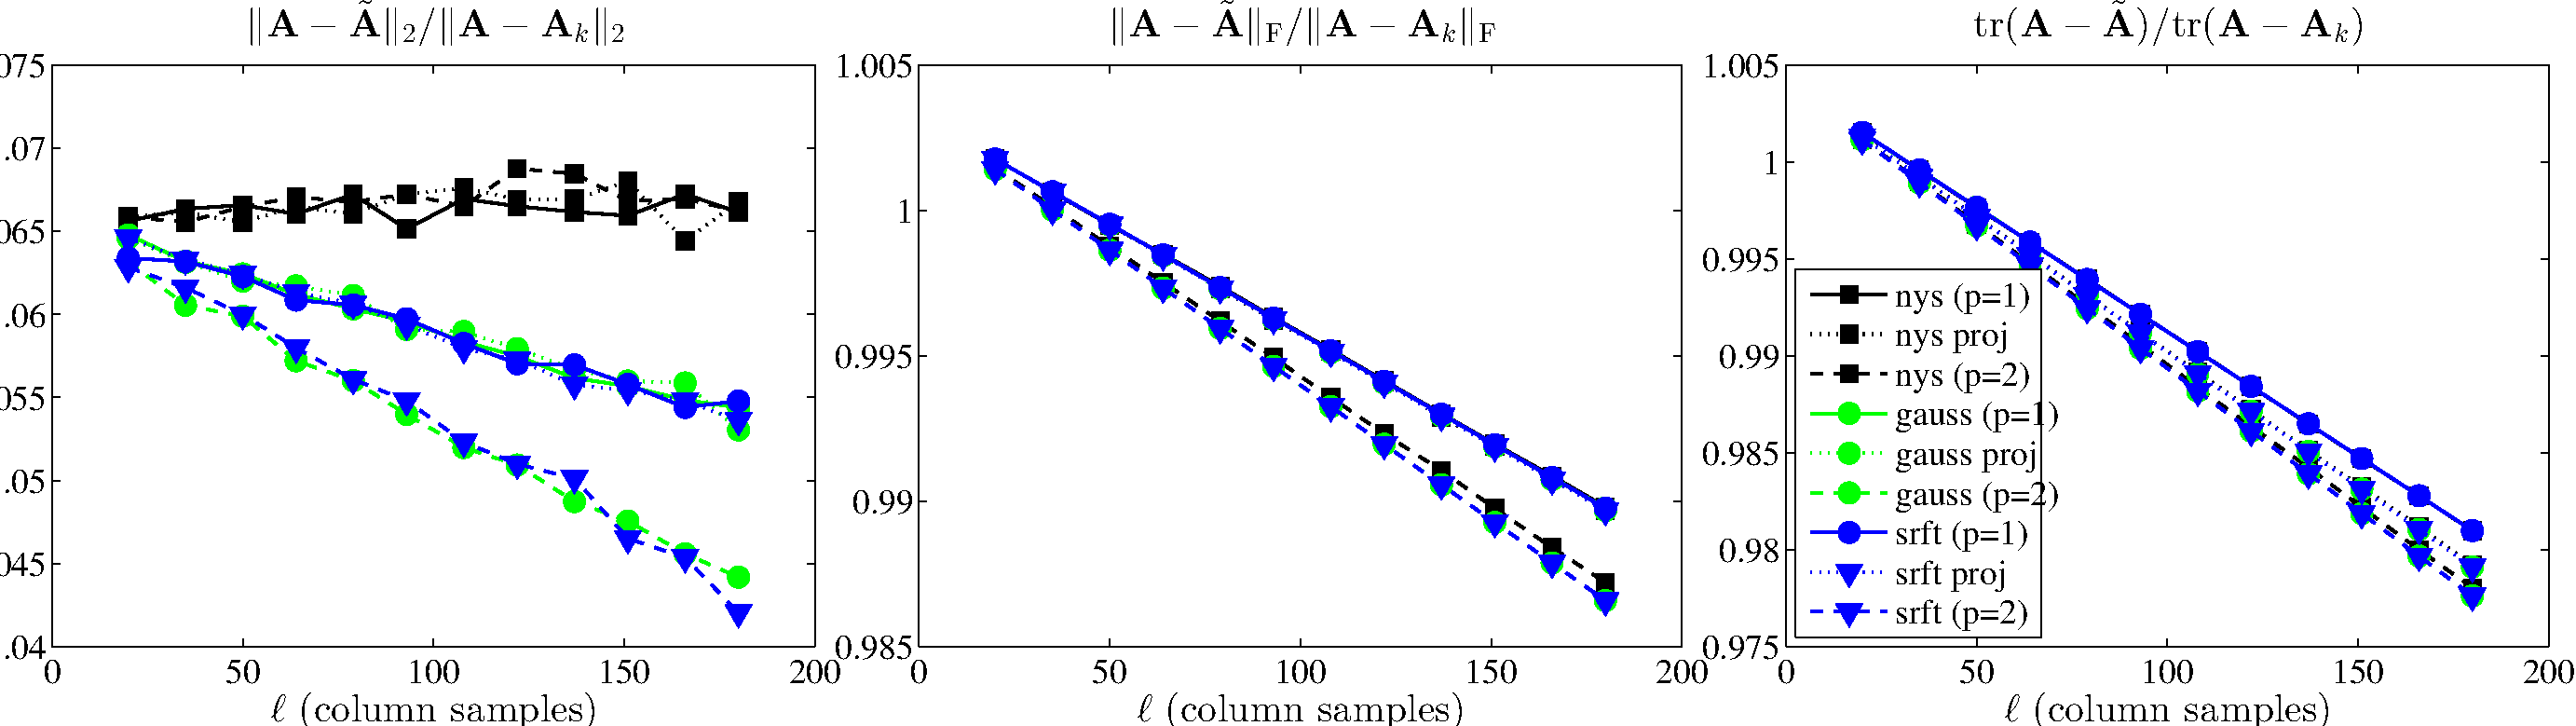
\includegraphics[width=6in, keepaspectratio=true]{figures/ch4/Gnutellarank20-eigexact-methods-nonfixed-rank-errors-with-eig}}
 
 \subfigure[Dexter, $k=8$]{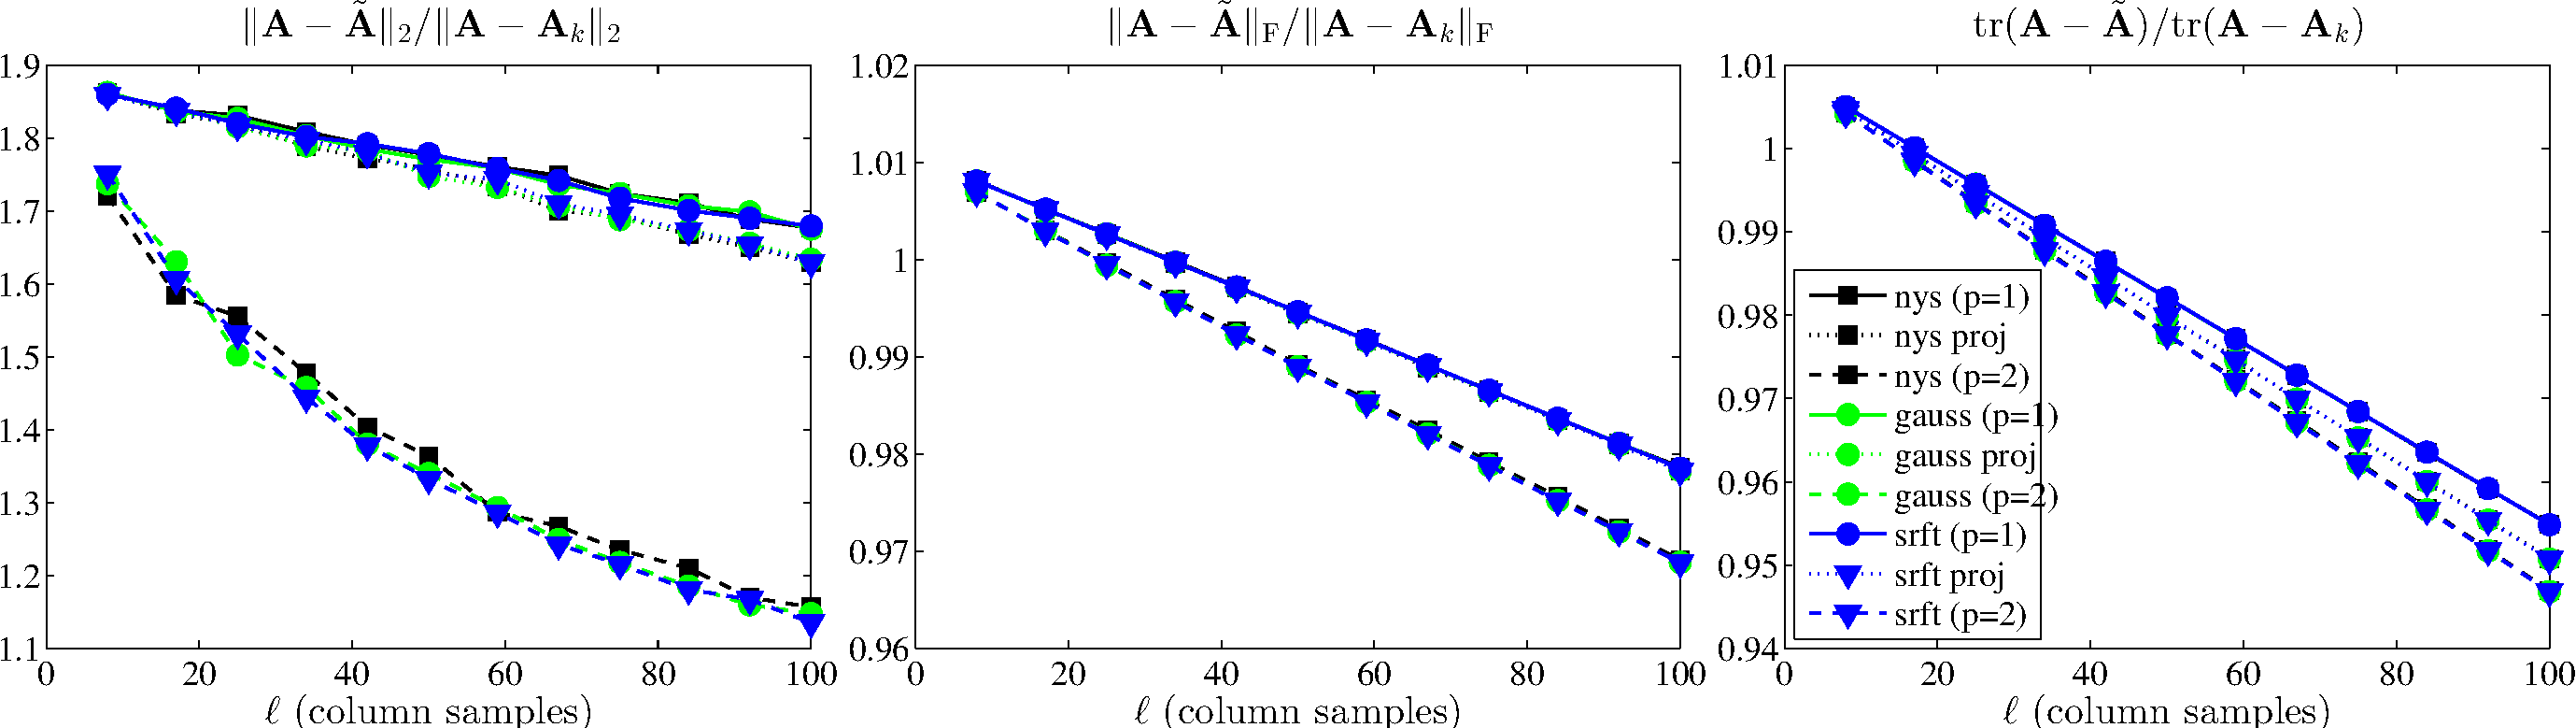
\includegraphics[width=6in, keepaspectratio=true]{figures/ch4/Dexterrank8-eigexact-methods-nonfixed-rank-errors-with-eig}}
 
 \subfigure[AbaloneD, $\sigma = .15, k = 20$]{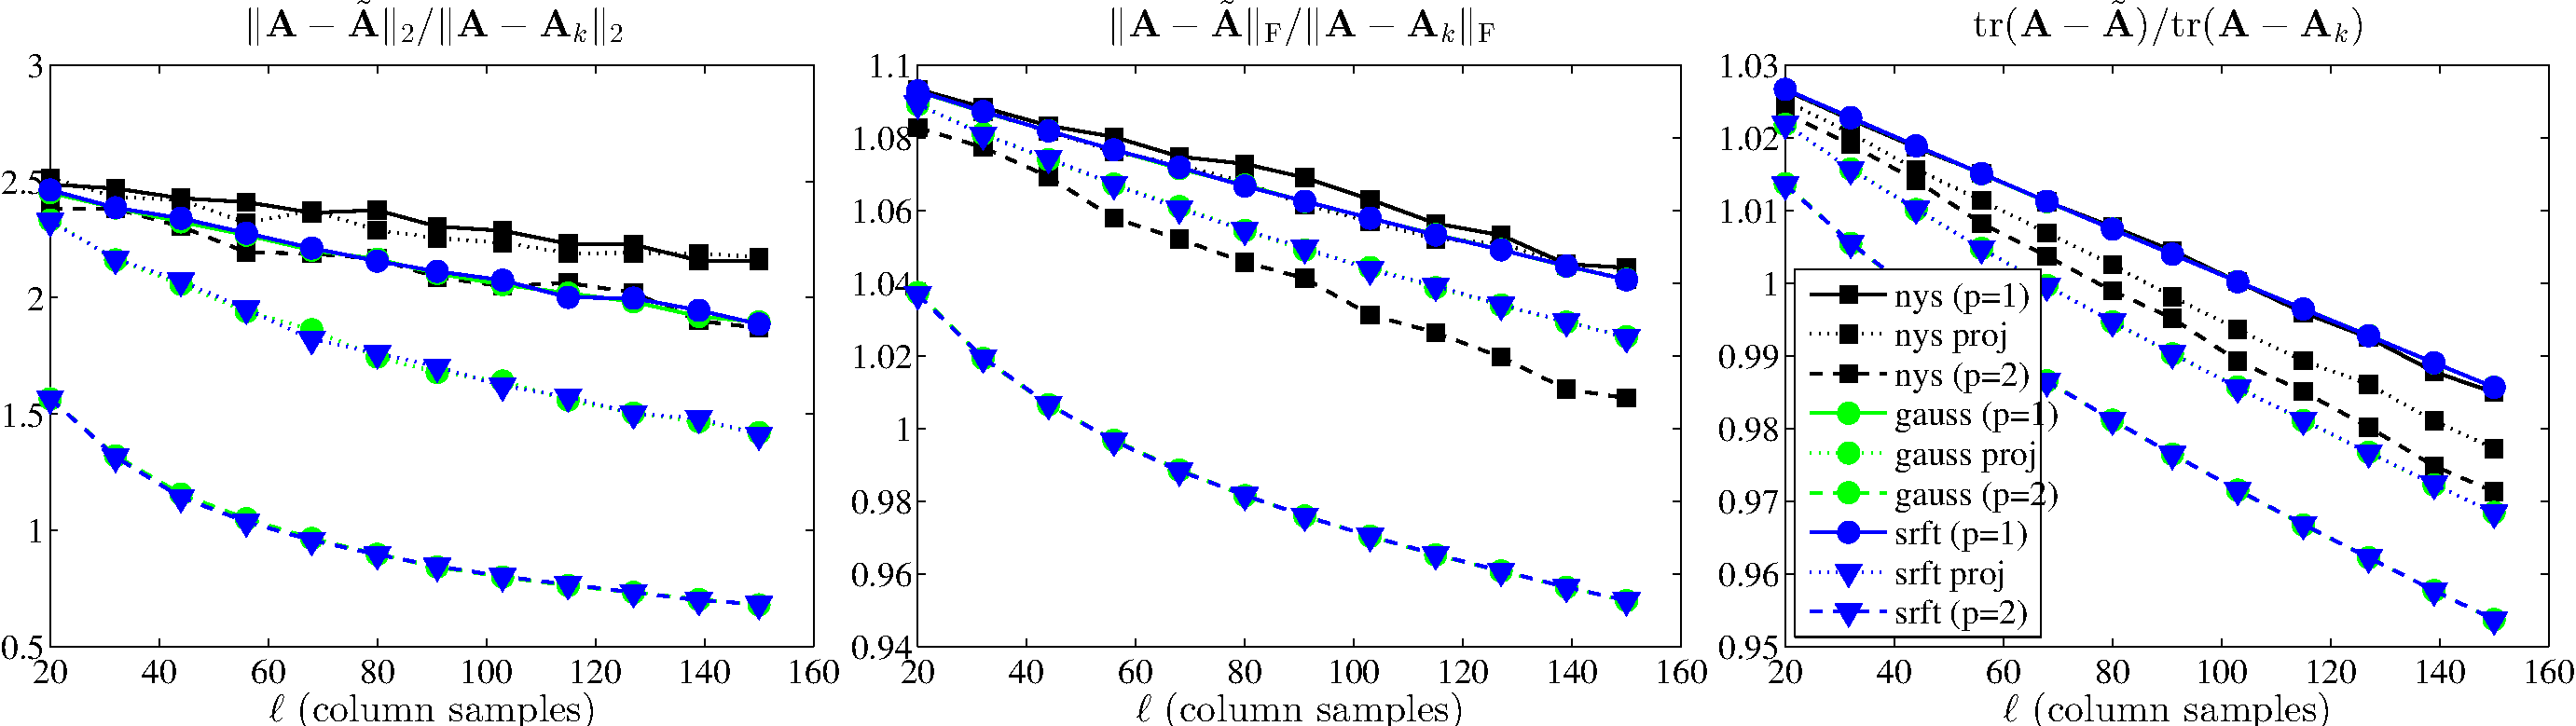
\includegraphics[width=6in, keepaspectratio=true]{figures/ch4/Abalonesigmapt15-eigexact-methods-nonfixed-rank-errors-with-eig}}
 
 \subfigure[WineS, $\sigma=1, k=20$]{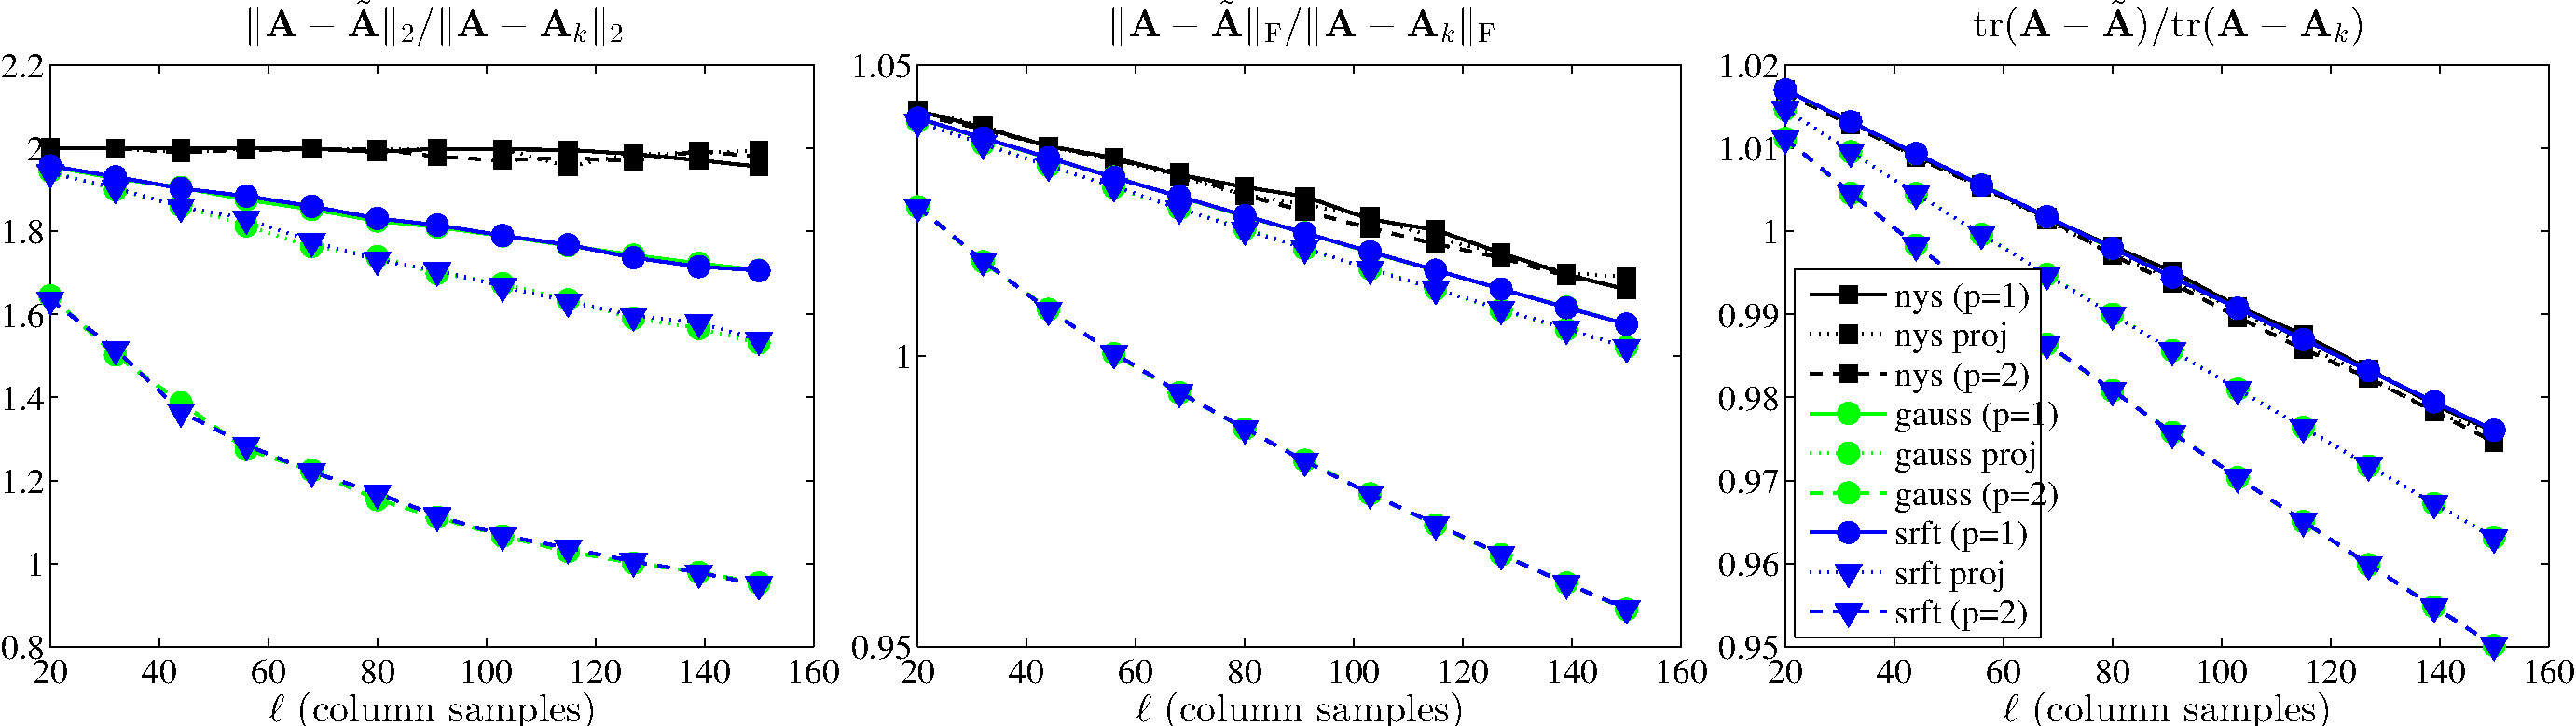
\includegraphics[width=6in, keepaspectratio=true]{figures/ch4/Winecompactsigma1-eigexact-methods-nonfixed-rank-errors-with-eig}}
 \caption[Comparison of projection-based low-rank approximations with one-pass SPSD sketches]{%
 {\sc Comparison of projection-based low-rank approximations with one-pass SPSD sketches.}
 The relative spectral, Frobenius, and trace-norm errors~\eqref{ch4:eqn:relerr1} of several
 non-rank-restricted SPSD sketches, including the pinched and prolonged low-rank approximants, 
 as a function of the number of columns samples $\ell$, 
 for several matrices from Table~\ref{ch4:table:datasets}. }%
 \label{fig:pinched-and-prolonged-approximants}
\end{figure}

Finally, we consider the performance of two projection-based SPSD sketches 
proposed in~\cite{HMT11}. Recall from Chapter~\ref{ch3} that these
low-rank approximations are constructed by forming an approximate basis $\matQ$ for 
the top $k$-dimensional eigenspace of $\matA$ and then restricting $\matA$ to that eigenspace. 

Given a sampling matrix $\matS,$ form the matrix 
$\matY = \matA \matS$ and take the QR decomposition of $\matY$ to obtain 
$\matQ,$ a matrix with orthonormal columns. The first projection-based approximant
mentioned in~\cite{HMT11}, which we eponymously refer to as the \emph{pinched} approximant, is simply $\matA$ pinched 
to the space spanned by $\matQ:$ 
\[
 \matP_{\matA \matS} \matA \matP_{\matA \matS} = \matQ (\matQ\transp \matA \matQ\transp) \matQ.
\]
Note that this approximant requires two passes over $\matA$. The second approximant, which 
we refer to as the \emph{prolonged} approximant, is 
\[
\matA \matQ (\matQ\transp \matA \matQ)^\pinv \matQ\transp \matA.
\]
The computation of a prolonged approximant also requires two passes over $\matA.$

It is clear that the prolonged approximant can be constructed using our SPSD 
sketching model by taking $\matQ$ as the sketching matrix. In fact, a stronger
statement can be made. Recall, from Lemma~\ref{ch4:lem:proj-form-of-sketch},
that for any sketching matrix $\matX,$ when 
$\matC = \matA \matX$ and $\matW = \matX\transp \matA \matX,$
\[
 \matC \matW^\pinv \matC\transp = 
 \matA^{1/2} \matP_{\matA^{1/2} \matX} \matA^{1/2}.
\]
By considering the two choices $\matX = \matA \matS$ and $\matX = \matQ$, we 
see that in fact the prolonged approximant is exactly the two-pass SPSD sketch:
\begin{align*}
 \matA \matQ ( \matQ\transp \matA \matQ)^\pinv \matA \matQ & = 
 \matA^{1/2} \matP_{\matA^{1/2} \matQ} \matA^{1/2} \\
 & = \matA^{1/2} \matP_{\matA^{1/2} (\matA \matS) } \matA^{1/2} \\
 & = \matA^2 \matS (\matS\transp \matA^3 \matS)^\pinv\matS\transp \matA^2.
\end{align*}
It follows that the bounds we provide in Section~\ref{ch4:sec:structuralresults} on the 
performance of multi-pass sketches pertain also to 
prolonged approximants. In particular, the additional errors of these approximants
are expected to be at least a factor of $\lambda_{k+1}(\matA)/\lambda_k(\matA)$
smaller than the additional errors of one-pass sketches.

In Figure~\ref{fig:pinched-and-prolonged-approximants}, we compare the empirical 
performances of several of the SPSD sketches considered earlier with  
pinched and prolonged approximants constructed using the same matrix $\matS.$
Specifically, we plot the errors of
pinched and prolonged approximants for choices of sketching
matrices corresponding to uniform column sampling, gaussian column 
mixtures, and SRFT-based column mixtures, along with the errors of one-pass
SPSD sketches constructed using the same choices of $\matS.$ In the
interest of brevity, we provide results only for a subset of the matrices 
listed in Table~\ref{ch4:table:datasets} and consider only the nonfixed-rank 
variants of the sketches.

Some trends are clear from Figure~\ref{fig:pinched-and-prolonged-approximants}.
\begin{itemize}
\item In the spectral norm, the prolonged approximants are considerably more accurate 
than the pinched approximants and one-pass sketches for all the matrices considered. Without 
exception, the prolonged Gaussian and SRFT column-mixture approximants are the most accurate
in the spectral norm, of all the schemes considered. Only in the case of the 
Dexter linear kernel is the prolonged uniformly column-sampled approximant nearly as
accurate in the spectral norm as the prolonged Gaussian and SRFT approximants. To
 a lesser extent, the prolonged approximants are also more accurate in the Frobenius
 and trace norms than the other schemes considered. The increased Frobenius and
 trace norm accuracy is particularly notable for the two RBF kernel matrices;
 again, the prolonged Gaussian and SRFT approximants are considerably more accurate
 than the prolonged uniformly column-sampled approximants.  
 \item After the 
 prolonged approximants, the pinched Gaussian and SRFT column-mixture approximants 
 have the smallest spectral, Frobenius, and trace-norm 
 errors. Again however, we see that the pinched uniformly column-sampled 
 approximants are considerably less accurate than the
 pinched Gaussian and SRFT column-mixture approximants. Particularly in the 
 spectral and Frobenius norms, the pinched uniformly column-sampled approximants
 are not any more accurate than the uniformly column-sampled sketches.
 \end{itemize}
It is evident that the benefits of pinched and
prolonged approximants are most dramatic when the spectral norm is the error metric,
and that Nystr\"om extensions do not benefit as much from multiple passes as do other
sketching schemes.

It is also evident that the pinched approximants
often yield a much slighter increase in accuracy over the one-pass sketches than do the
prolonged approximants. Recall that the prolonged approximants are simply
two-pass sketches. Our investigations point to the conclusion that two-pass sketches
are significantly more accurate than the projection-based low-rank approximations
that also require two passes over $\matA.$ Of course, one should temper this
comparison with the knowledge that projection-based low-rank approximations, unlike SPSD sketches, are stably computable.